\section{Soft robotics study cases}
\label{sec:C5:studycases}
In the subsequent section, we will dive into the capabilities of the toolkit, \texttt{Sorotoki}. To provide a comprehensive overview of the toolkit, various problem scenarios will be considered, each with specific problem settings aimed at the design, modeling, or control of soft robots. We will also focus on widely cited papers in the field of soft robotics and demonstrate these, mostly experimental, works using the \texttt{Sorotoki}.
\begin{rmk}
It is noteworthy that the full code can be accessed in the repository under the folder \texttt{./examples/paper/}, enabling users of the toolkit to reproduce all presented simulation results in the following section. Presets are found under the \texttt{./+preset/} folder.
\end{rmk}
%
\afterpage{
\begin{figure}[t]
\centering
\vspace{-3mm}
\includegraphics*[width=0.7\textwidth]{./pdf/thesis-figure-6-17.pdf}
%\input{./fig/fig_passivewalker_ref.tex}
\vspace{-1mm}
\caption{\small Snapsnots of the multi-legged passive walker from Suzumori and Saito \cite{Suzumori2008Sep} can be observed. The soft walker is placed on an inclined surface with a slope of $\varphi = -30\si{\degree}$ and initiates locomotion from an offset in the gravitational potential. These video frames were captured using a high-speed camera. Images from Suzumori et al. \cite{Suzumori2008Sep}, used with permission with rights belonging to \copyright2008 IEEE.
\label{fig:C5:passivewalker_true}}
\end{figure}
%
\begin{figure}[t]
\centering
%\vspace{-5mm}
\includegraphics*[width=.7\textwidth]{./pdf/thesis-figure-6-18.pdf}
%\input{./fig/fig_passivewalker_soro.tex}
\caption{\small Snaphots of the multi-legged passive walker from \texttt{Sorotoki}. The experimental setup is similar to that described in \cite{Suzumori2008Sep}. By comparing the gaits in Fig. \ref{fig:C5:passivewalker_true}, a resemblance can be seen between the results obtained in \texttt{Sorotoki} and those reported in \cite{Suzumori2008Sep}. The Von Mises stress as shown by \protect\colormapcaption{0}{.75cm}$\!\!\in [0,100]$ \si{\mega \pascal}. }
\label{fig:C5:passivewalker_soro}
\end{figure}
\clearpage
}
%
\subsection{Multi-legged soft passive walker}
\label{sec:C5:suzumori_walker}
In the first case study, the \texttt{Sorotoki} toolkit will be used to examine the dynamics of a multi-legged soft passive walker. The work of Suzumori and Saito \cite{Suzumori2008Sep} served as a key source of inspiration for this modeling problem. They proposed using a specialized soft structure that consists of an array of V-shaped soft legs, which exhibit stable intrinsic locomotion when placed on an inclined surface. This behavior was observed in experiments, as shown in Figure \ref{fig:C5:passivewalker_true}. The natural locomotion is driven by the elastic deformations of the V-shaped legs and their interaction with the environment, and is propelled forward by gravity. To increase the amplitude of these harmonics, small weights are placed at intermediate locations on the connecting soft body between pairs of V-shaped legs. Each pair of soft legs is tuned to a natural resonance frequency, and when coupled in parallel through a central deformable elastic body, synchronization occurs between the legs during locomotion. In other words, after a transient period, each leg pair will converge to a similar limit cycle, but with a unique phase offset relative to its neighbors.

The objective of this study is to reproduce the dynamics of the soft passive walker described in Suzumori et al. \cite{Suzumori2008Sep} using \texttt{Sorotoki}. In the work of Suzumori et al. \cite{Suzumori2008Sep}, the material parameters of the soft passive walker were given as: Young's modulus $E_0 = 1.2$ \si{\mega \pascal}, Poisson ratio $\nu_0 = 0.49$, and density $\rho_0 = 3600 \cdot 10^{-12}$ \si{\kilo \gram \per \milli \metre \cubed}. Since the material model is not exactly specified in \cite{Suzumori2008Sep}, a Neo-Hookean model was utilized with Rayleigh damping $\zeta = 1.5$.

To design the geometry of the V-shaped soft legs, the \code{sStrut(V1,V2,W)} function was utilized. This function generates an element of the \code{Sdf} class, requiring two nodal positions \code{V1,V2} and the strut's width \code{W} as input. The function was used to assemble a pair of legs iteratively, using the union operator implemented as {MATLAB}'s '\code{+}' arithmetic. The legs were then horizontally repeated three times with a uniform spacing of $25$ \si{\milli \metre}. A coupling soft body was added, along with two weights at intermediate locations. The resulting SDF is first converted to an \code{.png} template and the imported in the \code{msh = Mesh('SDF.png','ElementSize',1.0)} to generate the finite element mesh. %The code for the implicit modeling routine is given below

% \begin{lstlisting}[style=matlab] 
% sdf = Sdf([]);
% for i = 1:numel(Pts)
%     sdf = sdf + sStrut(Pts{i,1},Pts{i,2},1);
% end

% R = sRectangle(2).rotate(pi/4);
% W = R.translate([25,11]) + R.translate([50,11]);

% sdf = sdf.repeat([25,0],3) + ... 
%         sStrut([12,11],[62,11],1) + W;

% sdf.export('SDF.png');        
% \end{lstlisting}

The mesh is then utilized to construct the finite element model, \ie, \code{fem = Fem(msh)}. The timestep for the implicit solver is set at $\Delta t = 0.33$ \si{\milli \second}, which is set using \code{fem.setTimeStep(dt)}. Instead of modeling the inclined surface, which would also require rotating the mesh, the direction of the gravitational acceleration vector is modified as follows: $g := \textrm{Rot}_y(\varphi) a_g$ with $\varphi = -\frac{\pi}{6}$ (rad). The gravitational acceleration is then added using the class function \code{fem.addGravity}. The inclined surface is modeled as a horizontal line SDF, which is used as a contact environment for the FEM model through the function \code{fem.addContact}. It should be noted that in Figure \ref{fig:C5:passivewalker_true}, the soft walker is held in place by two fingers, which results in initial deformations of the soft body and nonzero initial conditions for the dynamic locomotion. To account for this, the mesh is pinned at the grasp locations, and the initial quasi-static deformations are solved for using \code{fem.solve}. Finally, the forward dynamics are solved implicitly using a Newmark-$\beta$ solver by calling the routine \code{fem.simulate}.

%
\begin{figure}[!t]
    \centering
    \includegraphics*[width=.99\textwidth]{./pdf/thesis-figure-6-19-1.pdf}
    %\includegraphics*[width=.495\textwidth]{./pdf/thesis-figure-6-19-2.pdf}
    %% This file was created by matlab2tikz.
%
%The latest updates can be retrieved from
%  http://www.mathworks.com/matlabcentral/fileexchange/22022-matlab2tikz-matlab2tikz
%where you can also make suggestions and rate matlab2tikz.
%
\definecolor{mycolor1}{rgb}{0.83922,0.84314,0.85098}%
\definecolor{mycolor2}{rgb}{0.06275,0.35686,0.84706}%
\definecolor{mycolor3}{rgb}{0.86667,0.21176,0.10980}%
%
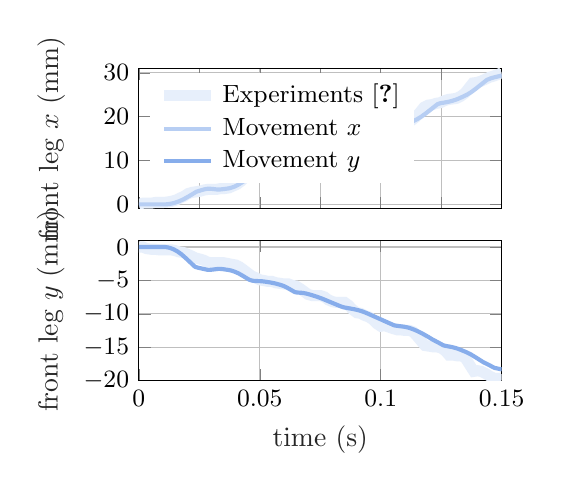
\begin{tikzpicture}

\begin{axis}[%
ylabel style={yshift=7pt},
width=0.38\textwidth,
height=0.147\textwidth,
at={(0\textwidth,0.18\textwidth)},
scale only axis,
xmin=0,
xmax=0.3,
xtick={0,0.05,0.1,0.15,0.2,0.25,0.3},
xticklabels={\empty},
ymin=-1,
ymax=31,
ylabel style={font=\color{white!15!black}},
ylabel={front leg $x$ (mm)},
axis background/.style={fill=white},
xmajorgrids,
ymajorgrids,
legend pos={north west},
legend style={legend columns=1, legend cell align={left}, align=left, draw=white},
ticklabel style={font=\small}
]
\addplot [color=mycolor1, line width=4.0pt]
  table[row sep=crcr]{%
0	0\\
0.0035458674481994	0.289056044065131\\
0.00690511177486641	0.289056044065131\\
0.0102643561015334	0.289056044065131\\
0.0136236004282004	0.433584584950562\\
0.016982844754871	0.433584584950562\\
0.020342089081538	0.433584584950562\\
0.023701333408205	0.557465894936438\\
0.027060577734872	0.701994435821874\\
0.0306997590887619	0.991050479887011\\
0.0340590034154289	1.44528540885432\\
0.037418411886776	1.85822276290534\\
0.040777656213443	2.47763346365765\\
0.04413690054011	2.74604331452895\\
0.047496144866777	2.89057081770866\\
0.0508553891934476	3.03509935859409\\
0.0542146335201146	3.3035092094654\\
0.057760500968314	3.44803671264511\\
0.061119745294981	3.44803671264511\\
0.064478989621648	3.44803671264511\\
0.067838233948315	3.63385867762393\\
0.071197478274982	3.63385867762393\\
0.074556722601649	3.77838721850936\\
0.077915966928316	4.19132872338329\\
0.0812752112549866	4.6042660774343\\
0.084821083393031	5.34755808817248\\
0.0881803277197015	6.37990199215288\\
0.0915395720463685	6.64831184302419\\
0.0948988163730355	6.91672480701269\\
0.0976048727395664	7.2470742751712\\
0.100964281210913	7.39160281605664\\
0.104323525537584	7.53613135694207\\
0.107682769864251	7.66001266692795\\
0.111042014190918	7.80454017010765\\
0.114401258517585	8.09359725187852\\
0.118040439871475	8.09359725187852\\
0.121399684198142	8.27942232997452\\
0.124758928524809	8.54783218084583\\
0.128118172851476	8.69236072173127\\
0.131477417178143	9.24982661666771\\
0.13483666150481	10.2615274405715\\
0.138195905831481	11.0048153004867\\
0.141555150158148	11.1493469544893\\
0.145101017606347	11.2938754953748\\
0.148460261933014	11.4384029985545\\
0.151819506259681	11.7481062735192\\
0.155178750586348	12.03716335529\\
0.158537994913015	12.03716335529\\
0.161897239239682	12.03716335529\\
0.165256483566349	12.1816908584697\\
0.1686158920377	12.5946323633437\\
0.172161764175744	13.3379202232589\\
0.175521008502415	14.7832056321133\\
0.178880252829082	15.9394349969025\\
0.182239497155749	15.9394349969025\\
0.185598741482416	15.794906456017\\
0.188957985809083	15.9394349969025\\
0.19231723013575	16.5381943159323\\
0.195676474462417	16.9511358208062\\
0.199222341910616	17.364074212563\\
0.201741775155618	17.6944236807215\\
0.205287642603817	18.1073620724782\\
0.208646886930484	18.2518937264808\\
0.212006131257152	18.2518937264808\\
0.215365375583819	18.3964212296605\\
0.218724619910486	18.3964212296605\\
0.222083864237156	18.6648310805318\\
0.225443108563823	19.1397090895758\\
0.22880235289049	19.8417076762206\\
0.23244169838906	20.9979328901869\\
0.235800942715727	22.1541622549761\\
0.239160187042394	22.6290444148429\\
0.242519431369061	22.7529257248288\\
0.245878675695728	23.0419817688939\\
0.249237920022395	23.1865103097794\\
0.252597164349062	23.6407410879238\\
0.255956408675733	23.9297971319889\\
0.259502280813777	24.0536825927977\\
0.262861525140448	24.1982111336831\\
0.266220769467115	24.6730891427271\\
0.269580013793782	25.3544363476494\\
0.272939258120449	26.5313119056324\\
0.276298502447116	27.6875412704216\\
0.279657746773783	27.8114225804075\\
0.28301699110045	28.1004796621784\\
0.286562858548649	28.5547145911457\\
0.289922102875316	28.9882991760962\\
0.293281347201987	29.2567079892618\\
0.296640755673334	29.5870584951261\\
0.300000000000001	30\\
};
\addlegendentry{\small Experiments \cite{Suzumori2008Sep}}

\addplot [color=mycolor2, line width=1.5pt]
  table[row sep=crcr]{%
0	0\\
0.0203343333333343	0.000204754783414529\\
0.0210030000000003	0.00204363054492518\\
0.0220060000000011	0.0112091005315342\\
0.023343333333333	0.0375453287409222\\
0.0250149999999998	0.0928428477122409\\
0.0273553333333325	0.211274155984835\\
0.03003	0.40389956991752\\
0.0333733333333335	0.728195711765675\\
0.0370510000000017	1.18863857989946\\
0.0413973333333324	1.86761313455635\\
0.0477496666666681	2.91273531571131\\
0.0530989999999996	3.36108093444547\\
0.0554393333333323	3.5182971367486\\
0.0567766666666678	3.56164236527315\\
0.057779666666665	3.57123142613126\\
0.0581139999999998	3.5750745585221\\
0.0584483333333345	3.57344177981586\\
0.0587826666666658	3.57666216522934\\
0.0611229999999985	3.52240362381116\\
0.0648006666666667	3.40004831242436\\
0.0658036666666675	3.39391796701808\\
0.0664723333333335	3.3988884785045\\
0.0674753333333342	3.41781341241822\\
0.0698156666666669	3.48990018002603\\
0.0741620000000012	3.64875308168606\\
0.0761679999999991	3.78423301080021\\
0.0788426666666666	4.03298738245142\\
0.0815173333333341	4.38158689868308\\
0.0848606666666676	4.94729572280232\\
0.0918816666666658	6.21171378662885\\
0.0938876666666673	6.37940404260633\\
0.095559333333334	6.44114411607609\\
0.0972310000000007	6.46624730211747\\
0.100574333333334	6.50837797934248\\
0.101911666666666	6.53940733088477\\
0.103917666666668	6.62012603843438\\
0.107595333333332	6.81805079485628\\
0.113279000000002	7.18607353321651\\
0.116622333333332	7.46480205787799\\
0.119297	7.77489564003703\\
0.122306000000002	8.25373995149281\\
0.128323999999999	9.27851191901776\\
0.129995666666666	9.40799388440388\\
0.131667333333333	9.46412767495504\\
0.135345000000001	9.55522973116796\\
0.137351000000002	9.65655142356811\\
0.139691333333335	9.83583525406738\\
0.146043666666667	10.4472362034769\\
0.150724333333333	10.9482632696932\\
0.155070666666667	11.5283171673102\\
0.165435000000002	13.0164047591208\\
0.168444000000001	13.2491742240621\\
0.174462000000002	13.5763496859077\\
0.177805333333332	13.7715705731124\\
0.181483	14.0656172405802\\
0.186163666666666	14.5250869389996\\
0.189841333333334	14.9968667692981\\
0.194856333333334	15.7837550364938\\
0.199536999999999	16.6505503391552\\
0.203548999999999	17.3631726667848\\
0.206558000000001	17.7218242543057\\
0.208898333333334	17.8799316692304\\
0.213913333333334	18.0856811261909\\
0.216922333333333	18.1977536470102\\
0.219262666666665	18.3270796047773\\
0.222605999999999	18.5766765104393\\
0.226283666666667	18.9298410039783\\
0.229292666666666	19.3091835252451\\
0.233304666666665	19.9543520298893\\
0.237651	20.8302096025582\\
0.247012333333331	22.8593422440506\\
0.249018333333332	23.051238820948\\
0.250689999999999	23.1396093625372\\
0.252361666666665	23.2048165608748\\
0.255704999999999	23.3832556082806\\
0.258379666666666	23.556065588102\\
0.262057333333331	23.8716677367953\\
0.265734999999999	24.2820027996296\\
0.271084333333331	24.9827788928645\\
0.274427666666664	25.5254671711257\\
0.278439666666664	26.33990213035\\
0.287800999999998	28.3877993174304\\
0.291144333333332	28.769449780818\\
0.293484666666664	28.9453728176913\\
0.300171333333331	29.3876780877625\\
};
\addlegendentry{\small Movement $x$}

\addplot [color=mycolor3, line width=1.5pt]
  table[row sep=crcr]{%
0	0\\
};
\addlegendentry{\small Movement $y$}

\end{axis}

\begin{axis}[%
width=0.38\textwidth,
height=0.147\textwidth,
at={(0\textwidth,0\textwidth)},
scale only axis,
xmin=0,
xmax=0.3,
xlabel style={font=\color{white!15!black}},
xlabel={time (s)},
ymin=-20,
ymax=1,
ylabel style={font=\color{white!15!black}},
ylabel={front leg $y$ (mm)},
axis background/.style={fill=white},
xmajorgrids,
ymajorgrids,
ticklabel style={font=\small},
xticklabels={,0,0.05,0.1,0.15,0.2,0.25,0.3},
]
\addplot [color=mycolor1, line width=4.0pt]
  table[row sep=crcr]{%
0	0\\
0.00323554164802431	0\\
0.0063788040002315	-0.240209060354363\\
0.00746424127104817	-0.268077693690039\\
0.00998490788999007	-0.333347079809126\\
0.0131281702421973	-0.333347079809126\\
0.016918828077106	-0.426721782878229\\
0.0198760914257043	-0.426721782878229\\
0.0231116377202198	-0.426721782878229\\
0.0269022955551286	-0.426721782878229\\
0.0298610039621856	-0.53340239622074\\
0.0330042663143928	-0.720153143342589\\
0.036794924149298	-0.826833756685105\\
0.0397536325563586	-1.05373757725788\\
0.0435442903912673	-1.34716826723042\\
0.0467798366857828	-1.64059895720296\\
0.0497385404463486	-1.77412807470663\\
0.0535277578692899	-1.97418406161007\\
0.0566710202214935	-2.26761475158261\\
0.0597220079243712	-2.36098945465171\\
0.0634203864634593	-2.36098945465171\\
0.0666559281114871	-2.36098945465171\\
0.070169752705425	-2.36098945465171\\
0.0734052943534529	-2.46767006799422\\
0.0763640027605099	-2.58789394571631\\
0.0801546605954186	-2.69457455905883\\
0.0832979229476258	-2.98800524903137\\
0.0863474655920413	-3.37481131256483\\
0.0901381280734412	-3.90845173338356\\
0.0932813904256484	-4.33541087036795\\
0.0970720529070448	-4.62884223083231\\
0.100030756667614	-4.92227292080485\\
0.103174019019818	-5.01564829436578\\
0.106964681501218	-5.14917674137763\\
0.110015664557604	-5.14917674137763\\
0.113158931556299	-5.34923272828107\\
0.116763590387603	-5.44260810184199\\
0.119906852739806	-5.53598280491109\\
0.123697515221206	-5.53598280491109\\
0.126656218981775	-5.73603879181453\\
0.1298917606298	-5.84271940515704\\
0.133590143815379	-6.25637330235985\\
0.136641126871766	-6.6564846056749\\
0.139784389223973	-7.08344441315111\\
0.143575051705369	-7.28350040005455\\
0.146533755465938	-7.28350040005455\\
0.150322972888876	-7.28350040005455\\
0.153466239887571	-7.47025047668458\\
0.156517222943961	-7.89721028416079\\
0.160307885425357	-8.19064097413333\\
0.163451147777565	-8.29732158747585\\
0.166409851538134	-8.29732158747585\\
0.17020051401953	-8.29732158747585\\
0.173436055667555	-8.72428139495206\\
0.176394759428124	-9.31114344538896\\
0.18018542190952	-9.83147795593428\\
0.183328684261728	-9.92485332949521\\
0.186933343093028	-10.2584377634105\\
0.190076610091726	-10.4584937503139\\
0.19331215173975	-10.8452998138474\\
0.196825976333692	-11.4723149377352\\
0.200061517981716	-11.8591210012687\\
0.203204780333923	-11.7657456277078\\
0.206810884223682	-11.9926501187724\\
0.209954146575889	-12.192705435184\\
0.213744809057285	-12.3927614220874\\
0.216702072405884	-12.3927614220874\\
0.219939054465879	-12.4861361251565\\
0.223728271888817	-12.4861361251565\\
0.226686980295877	-12.68619211206\\
0.229830242648084	-13.2999019961662\\
0.233620905129481	-14.1269731069575\\
0.23657960889005	-14.7406836615555\\
0.240370266724955	-14.8473636044062\\
0.243605813019471	-14.9407389779671\\
0.24656451678004	-14.9407389779671\\
0.250353734202978	-15.1407949648706\\
0.253498441613644	-15.5677547723468\\
0.256455704962246	-16.181464656453\\
0.260246362797151	-16.181464656453\\
0.263481909091666	-16.2881452697955\\
0.266995729039117	-16.2881452697955\\
0.270231270687141	-16.674951333329\\
0.273374537685839	-17.5953971471894\\
0.27698063692911	-18.6092190051025\\
0.280123903927805	-18.5158436315416\\
0.283081167276404	-18.6092190051025\\
0.286871825111312	-18.9428034390178\\
0.290107366759337	-19.3296095025512\\
0.293898029240733	-19.6631939364665\\
0.296856733001302	-19.6631939364665\\
0.299594518557168	-20.0001020178042\\
};
%\addlegendentry{$\theta_1$}

\addplot [color=mycolor3, line width=1.5pt, forget plot]
  table[row sep=crcr]{%
0	0\\
0.0203343333333343	-0.000236429810705374\\
0.0210030000000003	-0.00235975652305598\\
0.0216716666666663	-0.00824431887495081\\
0.0226746666666671	-0.0258324238495504\\
0.0243463333333338	-0.0782442314001912\\
0.0263523333333318	-0.178647824314947\\
0.028692666666668	-0.346454018960404\\
0.0317016666666667	-0.640404186380266\\
0.0350450000000002	-1.06720243394641\\
0.0390569999999997	-1.71377980358588\\
0.0464123333333326	-2.96056648576507\\
0.0487526666666653	-3.09197641211778\\
0.0567766666666678	-3.41713537349301\\
0.057779666666665	-3.42286874319493\\
0.0584483333333345	-3.42160507517114\\
0.0591170000000005	-3.41614318497105\\
0.0607886666666673	-3.38590187400018\\
0.0654693333333327	-3.28094641852346\\
0.0664723333333335	-3.27691522480478\\
0.0671409999999995	-3.27911754070608\\
0.0681440000000002	-3.28906759086544\\
0.0694813333333322	-3.31422724334634\\
0.0744963333333324	-3.44869007428436\\
0.0765023333333339	-3.53272943073928\\
0.0791770000000014	-3.69308080592031\\
0.0825203333333349	-3.95681189260227\\
0.0858636666666683	-4.30919183085634\\
0.0912129999999998	-4.8914994566651\\
0.0935533333333325	-5.02895466039048\\
0.0952249999999992	-5.07329878719004\\
0.0965623333333347	-5.08871456449221\\
0.100908666666665	-5.11804112877142\\
0.102246000000001	-5.13838289503283\\
0.104920666666668	-5.20078832718069\\
0.108932666666668	-5.31604906293114\\
0.112610333333333	-5.44914215521236\\
0.117291000000002	-5.67836466798553\\
0.119965666666666	-5.85275971845817\\
0.122306000000002	-6.06232891215206\\
0.128992666666669	-6.7491477887606\\
0.130664333333335	-6.8040327341766\\
0.132336000000002	-6.82951936773133\\
0.134676333333335	-6.85742427913367\\
0.136348000000002	-6.89680345262662\\
0.138354	-6.96691307614919\\
0.142031666666668	-7.14780086216811\\
0.147046666666668	-7.43250136633203\\
0.151727333333334	-7.74388758585663\\
0.160420000000002	-8.39879054260952\\
0.167441	-8.92100117432673\\
0.169781333333333	-9.0444714319342\\
0.175799333333334	-9.23847593485696\\
0.178474000000001	-9.33115461094308\\
0.182151666666666	-9.49504053788379\\
0.185495	-9.68328671735593\\
0.189506999999999	-9.9826751200816\\
0.211238666666667	-11.734191699557\\
0.213578999999999	-11.796607421519\\
0.219262666666665	-11.9289776050659\\
0.222271666666664	-12.0380883092023\\
0.224612	-12.1629604395797\\
0.228624	-12.4408405131591\\
0.233639	-12.8733606108324\\
0.239322666666666	-13.456559391608\\
0.243000333333331	-13.865234134065\\
0.247346666666665	-14.2669133670741\\
0.251693	-14.7089308312659\\
0.253030333333331	-14.7730256793178\\
0.258379666666666	-14.9585548280778\\
0.262057333333331	-15.1223077293774\\
0.264731999999999	-15.2815833008369\\
0.27075	-15.7329248586555\\
0.27409333333333	-16.0267222416297\\
0.278439666666664	-16.5072704530992\\
0.285126333333331	-17.2706639008532\\
0.287800999999998	-17.5023518094663\\
0.29415333333333	-18.0939501889633\\
0.300171333333331	-18.3209923712622\\
};
\end{axis}
\end{tikzpicture}%
    \caption{\small Comparison of the front leg rectilinear displacement between the experimental data obtained from Suzumori et al. \cite{Suzumori2008Sep} and the numerical data produced by \texttt{Sorotoki} shows that, although there are discrepancies, the step-like behavior and the traveled distance in the horizontal and vertical directions appear to be truthfully captured in comparison to the original experimental data. }
    \label{fig:C5:passivewalker_compare}
\end{figure}
%

Figure \ref{fig:C5:passivewalker_soro} shows snapshots of the dynamic simulation of the soft passive walker at times corresponding to those depicted in Figure \ref{fig:C5:passivewalker_true}. Although slight deviations are noticeable, the overall dynamic characteristics of the locomotion are captured closely by the dynamic FEM model produced using \texttt{Sorotoki}. To further demonstrate the validity of the model, a comparison of the rectilinear displacement of the front leg between the experimental data and the simulated model is presented in Figure \ref{fig:C5:passivewalker_compare}. The experimental data is obtained from \cite{Suzumori2008Sep} and is shown in Figure \ref{fig:C5:passivewalker_compare} (in gray). As demonstrated in the figure, the step-like behavior is accurately captured by the numerical model, and the horizontal and vertical distances traveled by the numerical model closely match the original experimental data.

To examine the gait cycle, we introduce state variables $\theta_1, \theta_2, \theta_3$ to represent the joint angles between the V-shaped legs, as depicted in Figure \ref{fig:C5:passivewalker_states}. The trajectory of these angles over a small time window of 200 \si{\milli \second} is shown in Figure \ref{fig:C5:passivewalker_gait}. The angular movements exhibit a clear and consistent "stable" gait cycle, indicating that synchronization indeed occurs between the deformable soft legs due to their interaction with the deformable soft body. An analysis of the stable gait cycle reveals a gait period of approximately $T_{\textrm{gait}} \approx 47.5$ \si{\milli \second} or $f_{\textrm{gait}} \approx 21.1$ \si{\hertz}.
%
\begin{figure}[!t]
    \centering
    \def\svgwidth{0.65\textwidth}
    %\input{./pdf/thesis-figure-6-20.pdf_tex}
    \input{./fig/walker_states.pdf_tex}
    \caption{\small Definition of the angular deflection of the three pairs of soft legs, denoted by $\theta_1$, $\theta_2$, and $\theta_3$, respectively. It should be noted that each pair has an intrinsic V-shaped structure, thus their stable equilibrium position during rest is approximately $\theta_i^\star \approx 45$ \si{\degree}. Image from \cite{Suzumori2008Sep}, used with permission with rights belonging to \copyright2008 IEEE.}
    \label{fig:C5:passivewalker_states}
    \vspace{-2mm}
    \end{figure}
    %
    \begin{figure}[!t]
        % This file was created by matlab2tikz.
%
%The latest updates can be retrieved from
%  http://www.mathworks.com/matlabcentral/fileexchange/22022-matlab2tikz-matlab2tikz
%where you can also make suggestions and rate matlab2tikz.
%
\definecolor{mycolor1}{rgb}{0.06275,0.35686,0.84706}%
\definecolor{mycolor2}{rgb}{0.86667,0.21176,0.10980}%
\definecolor{mycolor3}{rgb}{0.18039,0.52157,0.25098}%
%
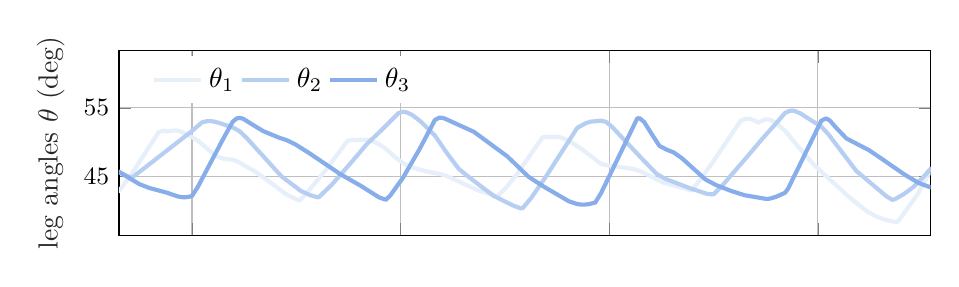
\begin{tikzpicture}

\begin{axis}[%
width=0.85\textwidth,
height=0.193\textwidth,
at={(0\textwidth,0\textwidth)},
scale only axis,
xmin=0.1825,
xmax=0.377,
xtick={0.2,0.25,0.3,0.35},
xticklabels={\empty},
ymin=-8.59436692696235,
ymax=18.3239448782706,
ylabel style={font=\color{white!15!black}},
ylabel={leg angles $\theta$ (deg)},
axis background/.style={fill=white},
xmajorgrids,
ymajorgrids,
legend style={at={(0.03,0.97)}, anchor=north west, legend columns=3, legend cell align=left, align=left, draw=white},
ticklabel style={font=\small},
ytick={0,10},
yticklabels={45,55},
]
\addplot [color=mycolor1, line width=1.5pt]
  table[row sep=crcr]{%
0.18232733333333	-2.30188806114205\\
0.185670666666663	0.459275592353302\\
0.192022999999995	6.45469561793443\\
0.193025999999996	6.66195442743467\\
0.193360333333329	6.65921840808779\\
0.194028999999995	6.5555266104338\\
0.194697666666663	6.60820549296253\\
0.195700666666662	6.69194226632872\\
0.196034999999995	6.69528570726732\\
0.19636933333333	6.6819861082615\\
0.197037999999996	6.60112221437848\\
0.198375333333329	6.24880761677116\\
0.199712666666663	5.81630902833377\\
0.201384333333328	5.24237169854863\\
0.204058999999996	3.83326166695333\\
0.206064999999995	2.88610248136889\\
0.207402333333329	2.59302865306167\\
0.208739666666663	2.49881047847044\\
0.209742666666662	2.41237009532592\\
0.210745666666663	2.22288328165492\\
0.215091999999995	0.722040098376267\\
0.217766666666662	-0.441187723043647\\
0.222781666666661	-2.70267968001193\\
0.225456333333328	-3.47832078647672\\
0.225790666666661	-3.51145240012962\\
0.227127999999995	-2.70716184273154\\
0.232142999999995	0.97357176516141\\
0.237157999999996	5.08936787642631\\
0.238160999999995	5.30959472571692\\
0.238495333333328	5.31308582887572\\
0.239163999999995	5.26636589309751\\
0.240166999999994	5.34380430756146\\
0.240835666666662	5.35564130582321\\
0.241169999999995	5.35228842844412\\
0.241838666666661	5.32533456841504\\
0.242841666666662	5.21309474428492\\
0.244178999999994	4.89840154418357\\
0.246184999999995	4.16210444275104\\
0.249193999999994	2.53963069152192\\
0.251199999999994	1.70876712999936\\
0.253205999999995	1.2088422772361\\
0.256214999999994	0.72960511338518\\
0.258555333333328	0.445787407951396\\
0.260226999999995	0.221103966624442\\
0.261564333333327	-0.0959543266153204\\
0.268585333333327	-2.04853964605678\\
0.272262999999993	-2.76480734755721\\
0.272931666666661	-2.91092788040498\\
0.273265999999994	-2.90254662915706\\
0.275271999999994	-1.65876560646226\\
0.27794666666666	0.339897500734562\\
0.283964666666661	5.66761870508612\\
0.28496766666666	5.80119540860571\\
0.285301999999994	5.78174782468604\\
0.28597066666666	5.70645099061716\\
0.286973666666661	5.78293811389958\\
0.287642333333327	5.76914694228424\\
0.288645333333326	5.62418479653334\\
0.290316999999993	5.16969790605185\\
0.293325999999993	4.01072910407037\\
0.298006666666661	1.83427413982818\\
0.299343999999993	1.63061402527145\\
0.30402466666666	1.23152177722429\\
0.305696333333326	1.07403335455232\\
0.30703366666666	0.843941852381196\\
0.308705333333327	0.373493848674846\\
0.313051666666659	-0.948841368702242\\
0.315391999999992	-1.32249013866339\\
0.31806666666666	-1.75623823556179\\
0.319403999999993	-2.04124337053998\\
0.319738333333326	-1.98176021335137\\
0.32107566666666	-1.08452323685827\\
0.324753333333327	2.00079549913327\\
0.331439999999992	8.06561536712418\\
0.332442999999992	8.37045165308042\\
0.333111666666658	8.42170396853629\\
0.333445999999993	8.40695505399669\\
0.334114666666659	8.31124737344653\\
0.335786333333326	7.87210172909765\\
0.33712366666666	8.25688185505189\\
0.337792333333326	8.31975199430715\\
0.338126666666659	8.31062021073345\\
0.338795333333326	8.20315865741348\\
0.340132666666658	7.75266237107809\\
0.342138666666658	6.64737453913875\\
0.345147666666659	4.44582969355035\\
0.349159666666658	1.60023671520466\\
0.357852333333325	-3.22528985202773\\
0.361864333333326	-5.15798979533417\\
0.364204666666659	-5.92192787831371\\
0.366544999999991	-6.41233842020569\\
0.368550999999991	-6.66722902132105\\
0.368885333333324	-6.68081109516272\\
0.369553999999992	-6.33526404073638\\
0.373900333333324	-2.61990524968527\\
0.376574999999992	0.364538916581836\\
0.377243666666658	1.22782424001941\\
};
\addlegendentry{$\theta_1$}

\addplot [color=mycolor2, line width=1.5pt]
  table[row sep=crcr]{%
0.18232733333333	0.675693846359113\\
0.185336333333328	-0.207446154145433\\
0.186004999999996	-0.0224000402164197\\
0.199712666666663	6.47898683360164\\
0.202387333333329	7.8698042188238\\
0.20339033333333	8.03692744096534\\
0.204058999999996	8.06694032704262\\
0.204393333333329	8.06465381046829\\
0.205061999999996	8.02354024971086\\
0.206399333333328	7.8261886883933\\
0.210076999999995	7.06628623681928\\
0.211414333333328	6.58312216335324\\
0.213085999999995	5.61693346343316\\
0.221444333333329	0.00026951240937656\\
0.226124999999994	-2.14797475047549\\
0.228465333333329	-2.78641032494537\\
0.230136999999996	-3.06127152608822\\
0.230471333333329	-3.00544165506627\\
0.233480333333327	-1.24285120201434\\
0.238160999999995	2.01333735774821\\
0.241838666666661	4.66594806494535\\
0.245516333333327	6.79972973384551\\
0.249528333333327	9.25700774966644\\
0.250531333333328	9.41006149703277\\
0.250865666666661	9.40951322079902\\
0.251534333333328	9.32776203722642\\
0.25287166666666	8.93103030303899\\
0.254877666666662	7.96871134240189\\
0.258220999999994	5.96280582966518\\
0.260895666666661	3.57699672003774\\
0.263904666666662	1.10621107080511\\
0.266244999999994	-0.0477547569124965\\
0.269588333333328	-1.60733372156976\\
0.272262999999993	-2.83166848206738\\
0.276943666666661	-4.2648201727631\\
0.278615333333327	-4.63645709001102\\
0.27894966666666	-4.68147889891408\\
0.279283999999993	-4.63321286960095\\
0.281289999999993	-3.17273480471269\\
0.28496766666666	0.088258811962751\\
0.292322999999994	7.06264132616776\\
0.294328999999994	7.74806501588789\\
0.295666333333326	7.99820242610454\\
0.296334999999994	8.03393888755739\\
0.296669333333327	8.04701420578069\\
0.297672333333328	8.12761267104009\\
0.298006666666661	8.12373925151686\\
0.298675333333327	8.05719464421561\\
0.299343999999993	7.90245350036697\\
0.300681333333326	7.22622560643665\\
0.307702333333326	2.65961520914604\\
0.311379999999993	0.347261605490413\\
0.313385999999992	-0.34689018048407\\
0.319403999999993	-1.75311387133304\\
0.323415999999993	-2.55620607128782\\
0.324418999999994	-2.62495503389791\\
0.324753333333327	-2.6348023609097\\
0.32508766666666	-2.58801055762811\\
0.327093666666659	-1.34151889040844\\
0.332777333333325	2.66165712469937\\
0.336789333333325	5.55585482562344\\
0.339798333333325	7.61068733650742\\
0.342138666666658	9.24891142977132\\
0.343141666666659	9.54361657038241\\
0.343810333333325	9.60612408069685\\
0.344478999999993	9.53778347609907\\
0.345816333333326	9.1862063737032\\
0.350831333333325	7.24644044170658\\
0.352502999999992	6.16713494749201\\
0.359189666666659	0.80220770485626\\
0.366544999999991	-2.97276460431764\\
0.367882333333325	-3.43966833654254\\
0.368550999999991	-3.31687588330351\\
0.370556999999991	-2.62014999557953\\
0.372897333333325	-1.55266228679629\\
0.375571999999991	0.0834264253880619\\
0.377243666666658	1.25287386559878\\
};
\addlegendentry{$\theta_2$}

\addplot [color=mycolor3, line width=1.5pt]
  table[row sep=crcr]{%
0.18232733333333	0.717600466257823\\
0.18734233333333	-1.12336125008317\\
0.189682666666663	-1.68382799129681\\
0.194028999999995	-2.40349994308714\\
0.196703666666663	-2.95733593286807\\
0.197706666666662	-3.05042461837621\\
0.198040999999996	-3.06077444265231\\
0.198375333333329	-3.0602966538308\\
0.199043999999995	-3.01716933446926\\
0.199712666666663	-2.93498265570707\\
0.200046999999996	-2.82973789040526\\
0.201384333333328	-1.56717602544105\\
0.207402333333329	5.386705215489\\
0.209742666666662	7.95770960134133\\
0.210745666666663	8.46446439769358\\
0.211414333333328	8.51806227717149\\
0.211748666666661	8.49591028370535\\
0.212417333333329	8.35902187754938\\
0.214088999999996	7.71048628592366\\
0.217097999999995	6.59535302816322\\
0.220775666666661	5.66742514275992\\
0.222781666666661	5.26395804950295\\
0.224787666666662	4.66269980267884\\
0.228130999999994	3.37807076125966\\
0.235486333333329	0.343423228539917\\
0.240501333333327	-1.40543796523722\\
0.244847666666661	-3.07802722277846\\
0.246184999999995	-3.36354975284329\\
0.246519333333328	-3.38997267001193\\
0.247522333333327	-2.80239902765395\\
0.250531333333328	-0.248617986974157\\
0.254543333333327	3.97250916684895\\
0.258220999999994	8.22711815361191\\
0.259223999999994	8.55496086669\\
0.259558333333327	8.56542037899618\\
0.25989266666666	8.54900280115812\\
0.260561333333328	8.44355057827765\\
0.267582333333328	6.49570869720983\\
0.275606333333327	2.89798513578477\\
0.280621333333327	-0.0464903162346246\\
0.284298999999994	-1.50350820654257\\
0.290316999999993	-3.64249914666132\\
0.292322999999994	-4.05513850779698\\
0.293325999999993	-4.13277953489326\\
0.293660333333326	-4.13839183817663\\
0.293994666666659	-4.13682106195376\\
0.29499766666666	-4.07309299697302\\
0.296334999999994	-3.88421671431277\\
0.296669333333327	-3.81031744949013\\
0.298006666666661	-2.49500473262311\\
0.30201866666666	2.54448048563777\\
0.306699333333327	8.43530865945126\\
0.30703366666666	8.48087859138943\\
0.307367999999993	8.4527875431958\\
0.308370999999994	7.93270690832473\\
0.310042666666659	6.30973448305397\\
0.31204866666666	4.43340595949672\\
0.313720333333327	3.90719782178881\\
0.315391999999992	3.50659281207069\\
0.317397999999994	2.65970887270109\\
0.32308166666666	-0.468880795768708\\
0.325756333333326	-1.32450630531883\\
0.329433999999992	-2.18153517850421\\
0.332442999999992	-2.76083737195846\\
0.336454999999992	-3.18076806240274\\
0.337457999999993	-3.28629097112971\\
0.337792333333326	-3.29464487608161\\
0.338126666666659	-3.28609157213632\\
0.338795333333326	-3.21784337721025\\
0.340132666666658	-2.9557061476382\\
0.342138666666658	-2.40380216926117\\
0.342807333333326	-1.86601507893096\\
0.345481999999992	1.44838768027877\\
0.350831333333325	8.1158711302543\\
0.351834333333326	8.42669039339647\\
0.352168666666659	8.40587290289117\\
0.352837333333325	8.171597847932\\
0.354508999999991	7.01402734560831\\
0.356849333333326	5.53526991689526\\
0.358855333333326	4.8962439010684\\
0.362198666666659	3.83774486800922\\
0.364873333333325	2.74386056327569\\
0.370891333333326	0.211109440358809\\
0.374234666666657	-0.992551785312449\\
0.376574999999992	-1.51537710638664\\
0.377243666666658	-1.62411278110961\\
};
\addlegendentry{$\theta_3$}

\end{axis}
\end{tikzpicture}%
        % This file was created by matlab2tikz.
%
%The latest updates can be retrieved from
%  http://www.mathworks.com/matlabcentral/fileexchange/22022-matlab2tikz-matlab2tikz
%where you can also make suggestions and rate matlab2tikz.
%
\definecolor{mycolor1}{rgb}{0.06275,0.35686,0.84706}%
\definecolor{mycolor2}{rgb}{0.86667,0.21176,0.10980}%
\definecolor{mycolor3}{rgb}{0.18039,0.52157,0.25098}%
%
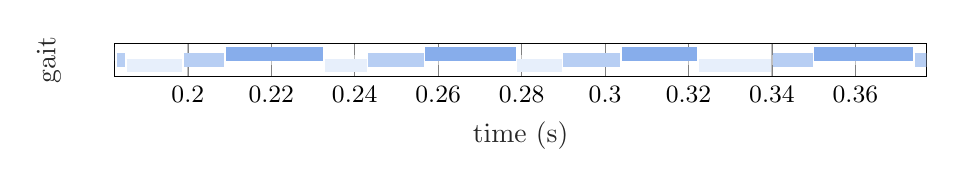
\begin{tikzpicture}
  \hspace{0.mm}
\begin{axis}[%
width=0.85\textwidth,
height=0.035\textwidth,
at={(0\textwidth,0\textwidth)},
scale only axis,
unbounded coords=jump,
xmin=0.1825,
xmax=0.377,
xlabel style={font=\color{white!15!black}},
xlabel={time (s)},
ymin=0.8,
ymax=1.4,
ytick={\empty},
ylabel style={font=\color{white!15!black}, yshift=16pt},
ylabel={gait},
axis background/.style={fill=white},
xmajorgrids,
ymajorgrids,
ticklabel style={font=\small}
]
\addplot [color=mycolor1, line width=5.0pt, forget plot]
  table[row sep=crcr]{%
0.185336333333329	1\\
0.198709666666662	1\\
nan	nan\\
0.232811666666662	1\\
0.242841666666661	1\\
nan	nan\\
0.27894966666666	1\\
0.289648333333327	1\\
nan	nan\\
0.322412999999993	1\\
0.339798333333326	1\\
};
\addplot [color=mycolor2, line width=5.0pt, forget plot]
  table[row sep=crcr]{%
0.182995999999996	1.1\\
0.185001999999996	1.1\\
nan	nan\\
0.199043999999996	1.1\\
0.208739666666662	1.1\\
nan	nan\\
0.243175999999995	1.1\\
0.256549333333328	1.1\\
nan	nan\\
0.28998266666666	1.1\\
0.303690333333327	1.1\\
nan	nan\\
0.340132666666659	1.1\\
0.349828333333325	1.1\\
nan	nan\\
0.374234666666658	1.1\\
0.377243666666658	1.1\\
};
\addplot [color=mycolor3, line width=5.0pt, forget plot]
  table[row sep=crcr]{%
0.182327333333329	1.2\\
0.182661666666663	1.2\\
nan	nan\\
0.209073999999995	1.2\\
0.232477333333328	1.2\\
nan	nan\\
0.256883666666661	1.2\\
0.278615333333327	1.2\\
nan	nan\\
0.30402466666666	1.2\\
0.32207866666666	1.2\\
nan	nan\\
0.350162666666659	1.2\\
0.373900333333325	1.2\\
};
\end{axis}
\end{tikzpicture}%
        \caption{\small Angular deflection of the V-shaped structure of the soft passive walker, simulated with \texttt{Sorotoki}. A clear gait cycle is observed in these deflections, indicating synchronization between the deformable structures due to the coupling of the soft body. By analyzing the stable gait cycles, a gait period of approximately $T_{\textrm{gait}} \approx 47.5$ \si{\milli \second} or $f_{\textrm{gait}} \approx 21.1$ \si{\hertz} is found.}
        \label{fig:C5:passivewalker_gait}
        \vspace{-6mm}
    \end{figure}
%
The numerical simulations presented in this study have effectively demonstrated the capabilities of the  \texttt{Sorotoki} framework in accurately capturing the complexities commonly encountered in dynamic analysis of soft robots. Furthermore, it has been demonstrated that the methodology proposed by Suzumori et al. \cite{Suzumori2008Sep} can be efficiently replicated using a minimal amount of code, specifically, approximately 30 lines within the \texttt{Sorotoki} framework.

\subsection{Computational design of bending PneuNet actuator}
\label{sec:C5:pneunet_opt}
In this section, we demonstrate the use of finite element models to aid in the design of PneuNet actuators, a popular type of soft robot actuator. PneuNet actuators, which have been in use since the 1980s, utilize a rectangular-shaped actuator with a stiffness differential to achieve a bending motion. Recent developments in the field, such as the work of Mosadegh et al. \cite{Mosadegh2014} and Ilievski et al. \cite{Ilievski2011Feb}, have proposed modern variations of PneuNet actuators that incorporate an inextensible but flexible bottom layer to further enhance the bending motion. The motion of a soft actuator depends on the interaction between the soft material, structural geometry, and the locations where external loads are applied. In their work, Mosadegh et al. \cite{Mosadegh2014} demonstrated the importance of geometry in the performance of PneuNet actuators by proposing a new design, called the fast PneuNet (fPN), that improved upon the earlier slower PneuNet (sPN) designs presented in \cite{Ilievski2011Feb}. The fPN design requires less gas for inflation and thus significantly increases the actuator's performance. Design optimization for PneuNet soft actuators remains an active area of research, as evidenced by recent studies \cite{Smith2022,Raeisinezhad2021May}.This demonstrates the continued interest in desing optimizing in soft PneuNet actuators, even decades after its initial development.

The purpose of this example is to demonstrate the use of \texttt{Sorotoki}'s design capabilities to optimize and create a PneuNet actuator. We will apply an inverse design method to find the optimal configuration of a soft material that undergoes pure bending when pressurized. This approach extends upon the work presented in Chapter \ref{chap: design}. To extend of our prior study, we aim to show that the optimized designs produced through this computational design method can effectively overcome the Sim2Real hurdles. To find the optimal material arrangement, we will use a nonlinear topology optimization technique, specifically designed for compliant mechanisms.

The objective in the nonlinear topology optimization approach is to find the optimal material distribution $\vec{\rho}^\star = \textrm{argmin}_{\vec{\rho}}  -\vec{L}^\top \vec{x}(\vec{\rho})$, where $\vec{L}$ is a sparse unit vector that selects the nodal displacements that promote bending motion. Once an optimum is found, the material distribution $\vec{\rho}^\star$ can be transformed into a 3D model and manufactured using a commercial 3D printing platform, such as Elastic 80A resin (Formlabs). The optimization algorithm can take into account the specific mechanical properties of the selected printing material, allowing for an optimal design that is tailored to these material properties.
%
\begin{figure}[!t]
    \vspace{-2mm}
    \centering
    \includegraphics*[width=.95\textwidth]{./pdf/thesis-figure-6-22.pdf}
    %\input{./fig/fig_opt_solutions.tex}
    \caption{\small Evolution of the topology-based optimization routine in \texttt{Sorotoki}. At $k=0$, we see the initial guess for the PneuNet actuator, and at $k=100$ we see a converged solution of the optimizer. Observe that the algorithm proposes a solution very similar to the PneuNet, but instead, it has a teardrop shape rather than the classical rectangular shape. It is worth mentioning that the optimizer accounts for the hyper-elastic material properties - in this case, Elastic 80A resin by Formlabs.}
    \label{fig:C5:fig_optpneunet_solutions}
    %\vspace{-3mm}
\end{figure}

\begin{figure}[!t]
    \centering
    %\input{./fig/fig_optpneunet_fem.tex}
    \includegraphics*[width=.95\textwidth]{./pdf/thesis-figure-6-23.pdf}
    \caption{\small Nonlinear finite element simulation of the optimized PneuNet actuator using \texttt{Sorotoki}. The system is subjected to a linear ramp upto 80 \si{\kilo \pascal}, and we observe the classical bending behavior of PneuNet actuators. The Von Mises stresses are shown as \protect\colormapcaption{0}{.75cm}$\!\!\in [0,10]$ \si{\mega \pascal}. }
    \label{fig:C5:fig_optpneunet_fem}
    \vspace{-3mm}
\end{figure}
%

To simplify the problem, we consider a single pressure chamber of the PneuNet actuator. To do this, a rectangular design domain with a size of $15 \times 30$ \si{\milli \meter} is defined using a \code{Sdf} library within \texttt{Sorotoki}. The \code{Mesh} class is then utilized to generate a mesh, which is used to construct a finite element model (FEM) using the \code{Fem} class. The \code{Fem} class takes several arguments to set up the optimization solver conditions, including the volume infill, penalty value, filter radius, time steps, and the maximum number of iterations for the method of moving asymptotes (MMA).

%
% \begin{lstlisting}[style=matlab] 
% fem = Fem(msh,'Infill', 0.33, 'Penal', 4, ... 
%     'FilterRadius', 2, 'TimeStep', 1/30, ... 
%     'MaxIterationMMA',70,'ChangeMax',0.05, ...
%     'OptimizationProblem','Compliant');
% \end{lstlisting}
%
The initial material distribution is set using \code{fem.initialTopology(sdf)} with \code{sdf = sCircle(5,[7.5,15])}, which creates a hole in the center of the actuator. The center element of the mesh is designated as an invariant pressure input and influences neighboring elements that satisfy the void conditions (i.e., $\rho_i \le \varepsilon$ with $\varepsilon = 0.1$) using an efficient flood-fill algorithm. The influenced void elements undergo synchronous volumetric expansion to simulate a positive pressure load. Given its similarities to muscular contraction, the syntax for this function is added as \code{fem.addMyocyte}. The material properties of the Elastic 80A resin from FormLabs are then specified using \code{fem.Material = Elastic80A} \cite{Xavier2022Jun}. Boundary conditions are added to the FEM model using the syntax \code{fem.addSupport}. Finally, the optimization routine is started using the \code{fem.optimize} command. %A code snippet is shown below:

% \begin{lstlisting}[style=matlab] 
% % ------------------------------------------------
% fem = Fem(msh,'TimeSteps',1/60);

% fem.Material = Elastic80A;
% fem = fem.initialTopology(sCircle(5,[7.5,15]));

% fem = fem.addSupport('Left',[1,1]);
% fem = fem.addSpring('Right',[0,1e-3]);
% fem = fem.addOutput('Right',[0,1]);
% fem = fem.addMyocyte('Center', 10 * kpa);

% fem = fem.optimize('Compliant',... 
%                    'MaxIteration', 100, ...
%                    'VolumeInfill', 0.3);
% % ------------------------------------------------
% \end{lstlisting}

The evolution of the material distribution during the first 100 optimization steps is depicted in Figure \ref{fig:C5:fig_optpneunet_solutions}. These interpolated isosurfaces are taken from the discrete FEM mesh and show the intermediate design solutions. Surprisingly, the optimization algorithm generates a design that is reminiscent of the fast PneuNet design presented by Mosadegh et al. \cite{Mosadegh2014}, but with a bellows-shaped pressure chamber in the form of an upside-down teardrop shape.

Next, the focus shifts to validating the optimization results. The aim is two-fold: $(i)$ to validate that the optimization algorithm indeed produces the desired bending motion, and $(ii)$ to verify if the design suggestion can be successfully transferred to reality (Sim2Real). To do this, the results of the optimization from \code{fem.optimize} are converted into a triangular mesh using \code{msh = fem.exportMesh}. Then, boundary conditions are assigned, such as a clamped boundary, gravitational loads, and internal pressure loads for each embedded PneuNet chamber. The same material model for \code{Elastic80A} resin is chosen. The quasi-static FEM simulation results of the optimized PneuNet actuator for linearly increasing pressure loads of $u = 80$ \si{\kilo \pascal} are shown in Figure \ref{fig:C5:fig_optpneunet_fem}. As can be seen, the desired bending behavior is achieved in the simulation.

\begin{figure}[!t]
    \centering
    %\input{./fig/fig_optpneunet_exp.tex}
    \includegraphics*[width=.825\textwidth]{./pdf/thesis-figure-6-24.pdf}
    \caption{\small Validation study of a 3D-printed \textit{PneuNet} actuator optimized using \texttt{Sorotoki}. The soft actuator is printed using SLA on a Form3+ printer using Elastic 50A UV-resin. Similar to the numerical simulations, we vary the pressure from 0 to 80 \si{\kilo \pascal} with a linear ramp. To measure the planar displacement, an orange marker is placed such that \texttt{Vision.m} can be employed.}
    \label{fig:C5:fig_optpneunet_exp}
\end{figure}

Next, the optimized isosurface shown in Figure \ref{fig:C5:fig_optpneunet_solutions} can be transformed into a 3D CAD model and printed as a physical soft actuator using a Form3+ SLA printer (FormLabs) with Elastic 80A resin. To validate its performance, the soft actuator is subjected to a linearly increasing pressure load of 80 \si{\kilo \pascal} in 5\si{\second} window. As seen in Figure \ref{fig:C5:fig_optpneunet_exp}, the optimized soft actuator successfully performs the desired bending motion, indicating the feasibility of crossing the Sim2Real barrier.

To quantify the discrepancies between the FEM predictions and the actual system, an optical marker is placed at the tip of the soft actuator. The spatial coordinates of the optical marker are obtained using the \class{Vision} class of \texttt{Sorotoki}, which uses the color-filtered Hough-space circle transformation to return the pixel coordinates of the marker. These measurements are collected using a RealSense D435 RGB-depth camera (Intel). To retrieve the spatial location of the color marker, we use the command \code{cam = Vision('realsense')} together with the function \code{cam.getMarker(R,rgb)}, where \code{R} is an estimate of the color marker radius in pixels, and \code{rgb} is the RGB color value of the marker.

\begin{figure}[!t]
    \centering
    %\input{./fig/fig_opt_compare.tex}
    \includegraphics*[width=.8\textwidth]{./pdf/thesis-figure-6-25.pdf}
    \caption{\small Comparison between the numerical simulation in \texttt{Sorotoki} and the experimental results where the orange marker is tracked using the Vision.m class is shown. The Von Mises stresses are shown as \protect\colormapcaption{0}{.75cm}$\!\!\in [0,10]$ \si{\mega \pascal}. The results indicate a close overall trend between the simulation and experiment. However, a discrepancy in the initial deformation ($u - 0$ kPa) is observed. It is hypothesized that this discrepancy is attributed to the inherent creep of SLA resin materials, which leads to a predeformed continuum due to the slow relaxation of the material upon actuation. }
    \label{fig:C5:fig_optpneunet_exp_compare}
\end{figure}

The comparison between the FEM predictions and experimental results is presented in Figure \ref{fig:C5:fig_optpneunet_exp_compare}. The deformation patterns of the FEM model and the physical system show close agreement, with an average error of $\pm 2$ \si{\milli \meter}. However, there is a noticeable difference in the initial conditions, as shown in Figure \ref{fig:C5:fig_optpneunet_exp_compare}. For $u = 0$ \si{\kilo \pascal}, under pure gravitational loads, the deformations deviate significantly. The cause of this discrepancy is believed to be related to post-curing and internal stress relaxation of the photopolymerization process. This suggests that the stress-free configurations of the FEM model and the physical system may differ, but accounting for this stress-relaxation phenomenon in photopolymer printing is outside the scope of this study and the \texttt{Sorotoki} toolkit.

Despite the presence of some differences, the numerical and experimental examples presented in this study highlight the ability of the computational design framework within \texttt{Sorotoki} to generate purposeful and useful material distributions with limited prior knowledge of conventional soft robotic design practices. This not only speeds up the design process, but it also opens up the possibility of creating new and innovative soft robot forms.

\subsection{Dynamic manipulation of high dexterity soft gripper}
\label{sec:C5:suzumori_gripper}
In this section, we will examine the use of reduced-order models for soft beams within the context of the \texttt{Sorotoki} software. These models are designed for efficient simulation by exploring minimal state representations of the dynamics of continuum systems. To demonstrate the capabilities of the soft beam modeling framework within \texttt{Sorotoki}, we will consider a specific example of a soft robotic system proposed by Suzumori and Suzuki in their seminal work \cite{Suzumori1991,Suzumori1992}. Despite being published in the early 1990s, the work by Suzumori et al. is still recognized as a seminal contribution to the field of soft robotics technology and remains relevant to this day.

In their research, Suzumori et al. developed a highly dexterous soft gripper consisting of four microfluidic soft actuators driven by an electro-pneumatic control system. Each finger has three internal pressure chambers, which together provide three controllable degrees of freedom at the fingertip, including pitch, yaw, and linear stretch. Unlike classic rigid grippers, the soft body of the gripper conforms to external forces, enabling intrinsic adaptation during grasping or manipulation tasks. As an illustration of the static grasping capabilities of this soft gripper, Figure \ref{fig:C5:suzumori_gripper_grasp} depicts two grasping configurations: a pinch grasp for a 40 \si{\milli \meter} diameter glass beaker (left) and a two-finger pair-pinch grasp for a 5 \si{\milli \meter} thick metal wrench (right). Suzumori et al. then employed inverse kinematic and compliance control to relate the tip position and compliance to input pressure values. As shown in Figure \ref{fig:C5:suzumori_gripper_grasp}, they were able to successfully hold and turn a 10 \si{\milli \meter} hexagonal bolt, with an average speed of 0.25 revolutions per second. Due to the wide range of dexterous actions performed by the gripper, the soft gripper proposed by \cite{Suzumori1991,Suzumori1992} remains a seminal contribution to the field of soft robotics, demonstrating the potential of the technology.
%
\begin{figure}[!t]
    \centering
    \includegraphics*[width=0.75\textwidth]{./pdf/thesis-figure-6-26-1.pdf}
    \includegraphics*[width=0.75\textwidth]{./pdf/thesis-figure-6-26-2.pdf}
    %\input{./fig/fig_suzugripper_old.tex}  \\[0.5em]
    %\input{./fig/fig_suzugripper_soro.tex}
    \caption{\small (top) Pinch and pair-pinch grasping configurations of the soft gripper proposed by Suzumori et al. \cite{Suzumori1992, Suzumori1991}. The high compliance of each soft finger allows for an adaptive, stable grasp that conforms to the shape of the rigid object. (bottom) A reconstructed soft gripper using the \texttt{Sorotoki} framework. To model each soft finger, we utilized the \class{Shapes} class and composed the entire gripper using the \class{Model} class. The rigid objects were modeled using the \class{Sdf} class. We observed a close resemblance between our simulation model and the original experiments performed by Suzumori et al. in \cite{Suzumori1991, Suzumori1992}. Used with copyright permission with rights belonging to \copyright1991 IEEE.}
    \label{fig:C5:suzumori_gripper_grasp}
    \vspace{-3mm}
\end{figure}

The objective of this investigation is to replicate the static grasping and dynamic bolt-screwing experiments as conducted by Suzumori in their published works \cite{Suzumori1991, Suzumori1992}, utilizing the \class{Sdf}, \class{Shapes}, and \class{Model} classes available in the \texttt{Sorotoki} software. The soft gripper's design specifications are based on the parameters provided by the available literature, which comprise a radius of $R_0 = 6$ (\si{\milli \meter}) and an assumed length of $L_0 = 80$ \si{\milli \meter} for each finger. Although the properties of the soft gripper's material are not mentioned explicitly, we suggest a Neo-Hookean model ansatz to address this issue. The proposed model has an elasticity modulus of $E_0 = 1.0$ \si{\mega \pascal}, Poisson ratio of $\nu_0 = 0.3$, and density of $\rho_0 = 2000 \cdot 10^{-12}$ \si{\kilo \gram \per \milli \metre \cubed}. The reduced-order model for each soft finger in interaction with a rigid object, denoted by $\Sigma_{\textrm{SR},i}$, is described by the following equation:
%
\begin{multline}
    \vec{M}(\q_i) \ddot{\q}_i  + \hB(\q_i,\dq_i)  =  \GB(\q_i) \pB_i +  \sum_{j\in \mathcal{S}_{\Omega_{\textrm{env}}}} \JB_{v,j}^\top(\q_i) \Big[ \FT_{{n},j}(\q_i) + \FT_{{t,j}}(\q_i,\dot{\q}_i)\Big],
    \label{eq:suzumori_fingermodel_lagrangian}
\end{multline}
%
where $\hB(\q_i,\dq_i)$ represents the collection of nonlinear internal forces, $\pB_i$ is the prescribed pressure input, $\JB_v(\q):= \lfloor\JB(L,\q)\rfloor_3$ is the linear velocity part of the generalized Jacobian matrix of the tip, $\mathcal{S}_{\Omega_{\textrm{env}}}$ represents the nodal indices that penetrates the object, and $
\FT_{{n}} = -\mu_e d \cdot \vec{e}_n$ and $\FT_{{t}} = -\mu_v |\FT_{{n}}| \, \textrm{sgn}(\dot{d}) \cdot \vec{e}_t$ 
denoting the normal and tangent contact forces between the $i$-th finger and the rigid object, respectively. The parameters $\mu_e, \mu_v > 0$ represent the contact coefficients. The distance between the finger and the object is given by $d = \texttt{sdf}_{\Omega_{\textrm{env}}}(\gammaB_L(\q))$, where $\texttt{sdf}_{\Omega{\textrm{env}}}(\cdot)$ represents the signed distance function of the rigid object and $\gammaB_L(\q)$ the finger's tip position. 

In this study, we utilize a third-order Chebyshev polynomial basis to model the deformation of the pneumatic soft robot's finger. The basis is sampled over $N_p = 100$ uniform nodes and is assembled into a matrix using the command \code{pod = Basis(100,3,'chebyshev')}. It is assumed that only free strains occur in the bending, while elongation and torsion are neglected. Each strain mobility vector is characterized by three modes of the Chebyshev basis, specified as \code{dof = [0,3,3,0,0,0]}, leaving the $\kappa_x$ and $\kappa_y$ curvatures free. The dynamic model for each finger is constructed using the command \code{shp = Shapes(pod,dof)}. The material properties are assigned using \code{shp.Material = NeoHookean(1.0, 0.3)}. To set the geometry of each finger, we call \code{shp.setLength(80)} to set its length, and \code{shp.setGeometry(sCircle(6))} to set a circular cross-section of radius $6$ (mm). Each finger of the soft gripper model is equipped with three fluidic chambers that are radially distributed along its circumference. As such, the input map $\GB$ for each finger becomes a nonlinear, non-square matrix. We assume that these distributed forces can be represented by a tangent bundle of linear forces that are positioned $3$ (mm) away from the center axis. To assign these forces, the \code{shp.addFluidic(@p)} command can be utilized, which requires an anonymous function \code{@p} that describes the path of the soft actuator. %A sample code for assembling one soft finger model is given below.

% \begin{lstlisting}[style=matlab] 
% dof = [0,3,3,0,0,0];
% pod = Basis(100,5,'chebyshev');

% shp = Shapes(pod, dof);
% shp = shp.setLength(80);
% shp = shp.setGeometry(sCircle(6));
% shp.Material = NeoHookeanMaterial(1.0, 0.3, ... 
%                 'Rho', 2000 * 1e-12);

% % for loop to assemble fluidic chambers
% for ii = 1:3
%     phi  = (ii - 1) * pi / 3
%     path = @(s)  3.0 * [cos(phi); sin(phi); s];
%     shp  = shp.addFluidic(path); 
% end

% shp = shp.rebuild(); % pre-assemble
% \end{lstlisting}

The full soft gripper model, composed of four identical finger \texttt{Shapes} classes, can be assembled using a for-loop routine. In this process, a class representing each finger is copied and assigned a unique $\textrm{SE}(3)$ base frame to each instance. Each finger is placed in a circular array with a radius of 37.5 (mm) relative to the center axis of the gripper body. The contact domain for each finger is specified using the method \code{shp.addContact(sdf)}, where \code{sdf} denotes the signed distance field of the contact object. For the beaker example, a cylindrical SDF with dimensions $40 \times 40 \times 60$ (mm) is considered, while for the wrench, a rectangular SDF with dimensions $5 \times 10 \times 100$ (mm) is used. Subsequently, each instance of the \class{Shapes} class is appended to the \class{Model} class constructor using the \code{mdl.addSystem(shp)}.

Once the global model of the soft gripper has been assembled, it can be controlled using an open-loop controller. In the case of a static grasping scenario with a glass beaker and wrench, we apply pressure ramps to each pressure chamber of the soft gripper through an auxiliary anonymous function, \code{@(mdl) Control(mdl)}. The function takes in a time variable and outputs a column vector of pressure signals, represented by $\vec{u} = (\vec{p}_1, \vec{p}_2, \vec{p}_3, \vec{p}_4)^\top$. The controller is then assigned to the Model class using the command \code{mdl.addControl(@Control)}, which is executed at each simulation step. The forward dynamics of the soft gripper's interaction with the object are implicitly solved through the \code{mdl.simulate()} routine. The simulated grasping configurations are shown in Figure \ref{fig:C5:suzumori_gripper_grasp}. It is evident that there is close agreement with the experiments in \cite{Suzumori1991,Suzumori1992}.

Subsequently, we aim to reproduce the hexagonal bolt screwing experiment of \cite{Suzumori1992,Suzumori1991}, which involves a more complex simulation than the previous scenario due to the dynamic interaction between the environment and the soft robot. To accurately depict this interaction, we must also incorporate dynamics into the signed distance field describing the hexagonal bolt screw. We assume a rotational mass-damper system, represented by the following equation:
%
\begin{align}
    I_\Omega\,\ddot{\theta} & = -\mu_\Omega \dot{\theta} -\sum_{i=1}^{N_{\textrm{finger}}} \!\!\sum_{j \in \mathcal{S}_\Omega} \rB_j (\q_i) \times \FT_{t,j}(\q_i,\dot{\q}_i) \cdot \vec{e}_3,                                                                      
    \label{eq:C5:screw}
\end{align}
%
where $I_\Omega = $ is the inertia of the hex-bolt, $\mu_\Omega = 2.5$ its friction coefficient, and $\rB$ the relative position vector from the point of contact and the central turning axis of the screw. Note that we only include the tangential force components $\FT_t$ that are responsible for motion, as the normal forces are assumed to have a net zero-torque contribution. The model described in equation \eqref{eq:C5:screw} is incorporated into the simulation by using the command \code{mdl.addSystem(@f)}, where \code{@f(x,u,t)} is an anonymous function that represents the state space. The required input \code{u} for equation \eqref{eq:C5:screw} is connected to the soft gripper by utilizing the \code{mdl.addController(@Controller)} command, which inputs tangential reaction forces into the screw model. The controller also includes the prescribed pressure profile $\pB_{1,2,3,4}$ for each of the four soft fingers.\\
%
% \begin{rmk}
% The inertia of the steel bolt $I_\Omega$ has been derived using standard ISO metric profiles of M10 screws. The screwing friction, however, has be determined using an ad-hoc approached, where the parameter has been tuned until desired behavior appears.\\
% \end{rmk}
% %

\afterpage{
\begin{figure*}[!t]
    \centering
    \includegraphics*[width=.85\textwidth]{./pdf/thesis-figure-6-27.pdf}
    %\input{./fig/fig_suzugripper_screw_old.tex} \\[0.5em]
    %\input{./fig/fig_suzugripper_screw_simulation.tex}
    \caption{\small (top) Snapshots of the bolt screwing experiment with the soft gripper, as presented in the work of Suzumori et al. \cite{Suzumori1991,Suzumori1992}, are displayed. The soft gripper periodically switches through a predefined set of configurations, enabling the holding and manipulation of a hexagonal bolt screw. In the experiment, a bolt turning rate of 0.25 rps was achieved. (bottom) The bolt screwing experiment was reproduced using \texttt{Sorotoki}. In the simulation, each finger was modeled utilizing the class \class{Shapes} and assembled together into \class{Model}. The contact interaction with the bolt was modeled using signed distance functions, and a rotational mass-damper model was used to describe the dynamics of the bolt. By utilizing solely the frictional interaction between the fingers and the screw, the experiment of Suzumori et al. was successfully reproduced.}
    \label{fig:C5:suzumori_gripper_screw}
    \vspace{-3mm}
\end{figure*}
\clearpage
}

%
\begin{figure}[!b]
    \centering
    \vspace{-3mm}
    \includegraphics*[width=.95\textwidth]{./pdf/thesis-figure-6-28.pdf}
    %% This file was created by matlab2tikz.
%
%The latest updates can be retrieved from
%  http://www.mathworks.com/matlabcentral/fileexchange/22022-matlab2tikz-matlab2tikz
%where you can also make suggestions and rate matlab2tikz.
%
\definecolor{mycolor1}{rgb}{0.06275,0.35686,0.84706}%
%
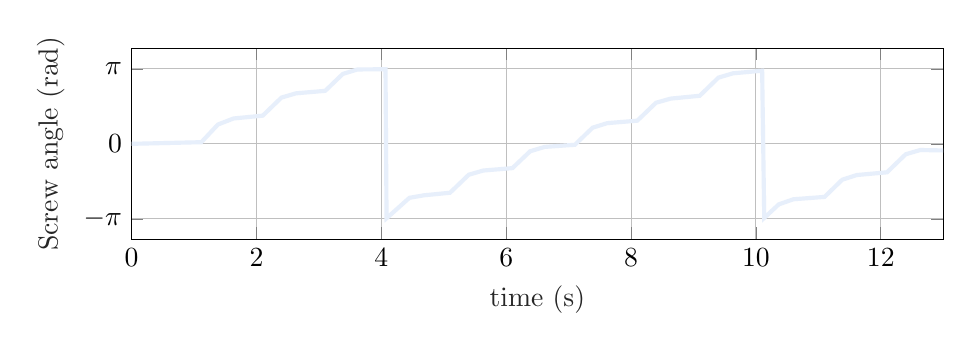
\begin{tikzpicture}

\begin{axis}[%
width=0.85\textwidth,
height=0.2\textwidth,
at={(0\textwidth,0\textwidth)},
scale only axis,
xmin=0,
xmax=13,
xlabel style={font=\color{white!15!black}},
xlabel={time (s)},
ymin=-4,
ymax=4,
ytick={-3.14159265358979,0,3.14159265358979},
yticklabels={{$\text{-}\pi$},{0},{$\pi$}},
ylabel style={font=\color{white!15!black}},
ylabel={Screw angle (rad)},
axis background/.style={fill=white},
xmajorgrids,
ymajorgrids
]
\addplot [color=mycolor1, line width=1.5pt, forget plot]
  table[row sep=crcr]{%
0	-0\\
1.11666666666667	0.0684561799806662\\
1.38333333333333	0.810083673385897\\
1.63333333333333	1.06283081427642\\
2.1	1.18049033665411\\
2.4	1.93768214421502\\
2.63333333333333	2.11624513955462\\
3.1	2.21949761075935\\
3.38333333333333	2.92926545847397\\
3.61666666666667	3.1152066309108\\
4.06666666666667	3.12666725738461\\
4.08333333333333	-3.12042668951522\\
4.45	-2.26157588158019\\
4.68333333333333	-2.15683409405717\\
5.1	-2.04949361229543\\
5.4	-1.29468976793778\\
5.63333333333333	-1.11842873292427\\
6.1	-1.0182276368425\\
6.38333333333333	-0.312059471745789\\
6.61666666666667	-0.129099657460664\\
7.1	-0.0403961247985567\\
7.38333333333333	0.675029276449868\\
7.61666666666667	0.86561269169994\\
8.1	0.970107811164747\\
8.4	1.72098481402045\\
8.63333333333333	1.89419158869196\\
9.1	2.01328325286623\\
9.4	2.77396164784034\\
9.63333333333333	2.95479172727074\\
10.1	3.06227813842414\\
10.1333333333333	-3.1036475913987\\
10.3666666666667	-2.53647629441526\\
10.6	-2.32302292439691\\
11.1	-2.22350029607539\\
11.3833333333333	-1.50252886320009\\
11.6166666666667	-1.30737812913506\\
12.1	-1.19342218066419\\
12.4	-0.436672999531943\\
12.6333333333333	-0.258898975296868\\
13.0166666666667	-0.277839760752059\\
};
\end{axis}
\end{tikzpicture}%

    \caption{\small The evolution of the hexagonal bolt angle $\theta(t)$ is depicted, where the stair-like trajectory of the screwing motion, as observed in Suzumori's experiment, is apparent. Through careful parameter and input shaping, a bolt-screwing motion of 0.16 rps was achieved. This is slightly slower than the reported rate of 0.25 rps, however, the underlying morphological characteristics are accurately captured.}
    \label{fig:C5:suzumori_gripper_screw_states}
\end{figure}

The qualitative comparison between the experiments conducted by Suzumori et al. \cite{Suzumori1991,Suzumori1992} and our numerical model programmed using \texttt{Sorotoki} is depicted in Figure \ref{fig:C5:suzumori_gripper_screw}. Similar to the simulation of the static object grasping scenario, the simulation of the Suzumori soft gripper's screwing experiment qualitatively reflects the real-world experiment performed in the 1980's. Not only do we observe similar deformation characteristics in the soft finger, but we also observe the step-like turning of the bolt screw, as reported in \cite{Suzumori1992}. To highlight these rotational trajectories, we present the rotation angle $\theta(t)$ in Figure \ref{fig:C5:suzumori_gripper_screw_states}, which shows that an average bolt-screwing speed of 0.16 rps is achieved. Although this rate is slightly slower than the reported rate of 0.25 rps, it is believed that the underlying morphological characteristics are accurately captured. Note that although the system is of highly complex nature, the simulation program contains less than 100 lines of code (including visualization).

\subsection[Environmental impedance control of soft manipulator]{Impedance control of soft robot manipulator with static environmental interaction}
The subsequent section will focus on the development of controllers utilizing the \class{Model} and \code{shapes} classes. In prior experiments, the Suzumori et al. gripper was governed in an open-loop fashion, with complications arising from the interplay between the model and dynamic object. Our investigation will now examine the feasibility of model-derived controllers in the \texttt{Sorotoki} scenario, drawing upon Della Santina et al.'s work \cite{DellaSantina2020a} as a prospective case study.

Their work presents a design for model-based controllers for soft robot manipulators, highlighting two control architectures: dynamic tracking and surface tracking. The authors proposed a Cartesian impedance controller for the latter architecture, which actively regulates the desired compliance behavior of the soft robot's end-effector in a static environment. Additionally, the work presented a contact path planning algorithm that initially brings the robot close to a desired setpoint on the surface (Phase 1: Approach), and then adjusts the setpoint to maintain contact with the surface (Phase 2: Explore). The proposed controller was validated both numerically and experimentally on a six-link soft robot manipulator, demonstrating that model-based controllers can lead to higher-level performances in soft robotic systems.

To maintain high computational bandwidth, the impedance controllers used in Della Santina et al.'s study \cite{DellaSantina2020a} incorporate an augmented rigid body model. This model employs Constant-Curvature kinematics to approximate the center of mass of the continuously deformable robot by projecting its mass distribution into a lumped mass description. This leads to an Euler-Lagrangian representation similar to the commonly used Denavit-Hartenberg (DH) parametrization models in rigid robotics. Moreover, this approach maintains classical properties, such as positive semi-definiteness of the inertia matrix and passivity properties, which are valuable for stability analysis.

Our aim in this section is to replicate the results of the closed-loop controlled multi-link soft robot during dynamic contact that were presented in the study by Della Santina et al. \cite{DellaSantina2020a}. Instead of employing the augmented rigid body model used in their work, we explore a reduced-order beam model, in which each link is represented as an inextensible, continuous PCC segment. This approach extends their work to a distributed mass robotic system. As a template for the soft manipulator model, we again utilize the \class{Shapes} class. According to \cite{DellaSantina2020a}, each CC segment of the soft manipulator has an intrinsic length of $\delta L_0 = 60$ mm and a mass of $m_0 = 334$ g. The robot has a rounded rectangular cross-section of 60 $\times$ 20 mm, which is described using \code{sdf = sSquircle}. The density of the soft robot manipulator, given its length and geometry, is approximated to be $\rho_0 = 1200 \cdot 10^{-12}$ (\si{\kilo \gram \per \milli \metre \cubed}). 

A crucial aspect of the simulation is the dynamic interaction with the environment. Therefore, a static environment must be assigned to the dynamic model. While \cite{DellaSantina2020a} presents multiple examples of dynamic contact, this study focuses on the experiment with a 40$^\circ$ slanted surface with wave indentations, as shown in Figure \ref{fig:C5:dellasantina_experiment}. The surface features were extracted from the image data presented in \cite{DellaSantina2020a} and the \code{env = sPolyLine(V)} function was used to generate the SDF environment, where \code{V} is a polyline vector. The environment is then added using \code{Shapes.addContact(env)}. Once all settings are assigned to the class \class{Shapes}, the model is constructed by \code{mdl = Model(Shapes)}. %The code for assembling the dynamic model is given below:

% \begin{lstlisting}[style=matlab]   
%  dof = [0,6,0,0,0,0];
%  pod = Basis(100,6,'pcc');

%  shp = Shapes(pod, dof);
%  shp = shp.setLength(60 * 6);
%  shp = shp.setGeometry(sSquircle(3, 3, 0.25));
%  shp = shp.addContact(sPolyLine(V));
%  shp.Material = NeoHookeanMaterial(1.0, 0.3, ... 
%                  'Rho', 1200 * 1e-12);

%  % build model (calls rebuild automatically)
%  mdl = Model(shp);
% \end{lstlisting}

Given the \class{Model} class, we can now start deriving the control law. For conciseness, let $\JB(\q) := \JB(L,\q)$ be the geometric Jacobian of the end-effector. We also introduce the Cartesian inertia matrix as $\LambdaB := (\JB^\top \MB \inv \JB^\top)\inv$. Then, the proposed Cartesian stiffness controller given in \cite{DellaSantina2020a} can be written as:
%
\begin{multline}
    \tauB = \JB^\top \Big[\JB_M^{+\top} \fB_{e} + \fB_{g} + \JB^\top \etaB_{\CB}(\IB - \JB_M^{+\top}\JB)\dq + \JB^\top(\KB_{c} (\gammaB_d - \gammaB_L) - \DB_c \JB \dq) \Big ],
    \label{eq:C5:dellasantina_controller}
\end{multline}
%
where $\gammaB_d$ and $\gammaB_L$ represent the desired and true end-effector positions, respectively; and $\KB_c$ and $\DB_c$ are the desired stiffness and damping of the end-effector. The closed-loop controller employs a so-called \textit{``dynamically consistent pseudo-inverse''} of the Jacobian, denoted as $\JB_M^{+}$, which is defined as $\JB_M^{+} := \MB^{-1} \JB^\top \LambdaB$. The controller also utilizes the Cartesian Coriolis terms, denoted as $\etaB_{\CB}(\q,\dq)$, which are expressed in the Cartesian frame and given by:
%
\begin{equation}
    \etaB_{\CB} = \LambdaB (\JB \MB\inv \CB - \dot{\JB}).
\end{equation}
%
The closed-loop controller, implemented as an anonymous function, is derived from four system matrices: the inertia matrix $\MB(\q)$, the Coriolis matrix $\CB(\q,\dq)$, the Jacobian $\JB$, and its time derivative $\dot{\JB}$. In \texttt{Sorotoki}, these matrices are automatically computed at each solver step and stored in a data structure named \code{shp.log}. The closed-loop controller can access this data structure. %A sample code of the controller is provided below:
%\vfill

% \begin{lstlisting}[style=matlab] 
% % ------------------------------------------------    
% function tau = Control(mdl)
%     % retrieve current log
%     log = mdl.System{1}.log;

%     J  = log.FK.J(:,:,end);        
%     dJ = log.FK.dJdt(:,:,end); 
    
%     Mi  = inv(log.EL.M);
%     Lam = inv(J * Mi * J.'); 
%     Eta = Lam * (J * Mi * log.EL.C - dJ);
%     Jmi = Mi * J.' * Lam;

%     if mdl.System{1}.isContact()
%         xd = [0.3637; 0.1406];
%     else
%         xd = [0.2307, 0.2576];
%     end

%     % impedance controller
%     tau = J.' * (Jmi.' * fe + fg + ... 
%         Eta * (log.I - Jmi.' * J) * log.dq + ...
%         (Kc * (xd - log.FK.p) - Dc * J * log.dq));
% end
% % ------------------------------------------------
% \end{lstlisting}

%
It is noteworthy that the controller above uses the command \code{shp.isContact} to detect if the robotic system is in contact. Similar to path planning in \cite{DellaSantina2020Jan}, upon contact, a new desired equilibrium position is adopted. These desired equilibrium positions for the end-effector are in line with the approach presented in \cite{DellaSantina2020a}. Subsequently, the implicit solver is invoked by calling \code{mdl.simulate} to solve the closed-loop dynamics. Snapshots of the dynamics have been presented in Figure \ref{fig:C5:dellasantina_experiment} which are produced by calling the function \code{shp.render}. Figure \ref{fig:C5:dellasantina_endeffector} shows the trajectory of the end-effector (dashed lines are the desired setpoints), Figure \ref{fig:C5:dellasantina_states} shows the evolution of the states, and Figure \ref{fig:C5:dellasantina_input} shows the control action $\tauB$ from \eqref{eq:C5:dellasantina_controller}.
%
\afterpage{
\begin{sidewaysfigure*}[!h]
    \centering
    \includegraphics*[width=0.95\textwidth]{./pdf/thesis-figure-6-29-1.pdf} \\[0.75em]
    \includegraphics*[width=0.95\textwidth]{./pdf/thesis-figure-6-29-2.pdf}
    %\input{./fig/fig_dellasantina_true.tex} \\[0.35em]
    %% This file was created by matlab2tikz.
%
%The latest updates can be retrieved from
%  http://www.mathworks.com/matlabcentral/fileexchange/22022-matlab2tikz-matlab2tikz
%where you can also make suggestions and rate matlab2tikz.
%
\definecolor{mycolor1}{rgb}{0.86667,0.21176,0.10980}%
\definecolor{mycolor2}{rgb}{0.06275,0.35686,0.84706}%
\definecolor{mycolor3}{rgb}{1.00000,0.16078,0.45882}%
\definecolor{mycolor4}{rgb}{0.68235,0.69020,0.70980}%
%
\begin{tikzpicture}

\begin{axis}[%
width=0.85\textwidth,
height=0.33\textwidth,
at={(0\textwidth,0\textwidth)},
scale only axis,
axis on top,
xmin=-310,
xmax=60,
xtick={\empty},
tick align=outside,
ymin=0,
ymax=400,
ytick={\empty},
axis background/.style={fill=white},
xmajorgrids,
ymajorgrids
]
\addplot [forget plot] graphics [xmin=-310, xmax=60, ymin=0, ymax=400] {fig_dellasantina_simu-1.png};
\addplot [color=mycolor1, only marks, mark size=2.0pt, mark=*, mark options={solid, mycolor1}, forget plot]
  table[row sep=crcr]{%
-140.6	353.7\\
};
\addplot [color=mycolor2, line width=1.0pt, forget plot]
  table[row sep=crcr]{%
-1	-4\\
-1.00000476565713	8.6\\
-1.00001906262853	21.1999999999928\\
-1.00004289091419	33.7999999999712\\
-1.00007625051412	46.3999999999279\\
-1.00011914142831	58.9999999998558\\
-1.00013267471724	71.5999999998672\\
-1.00011619124632	84.199999999875\\
-1.00006969101557	96.7999999998078\\
-0.999993174024978	109.399999999594\\
-0.999886640274549	121.999999999162\\
-0.999736120714447	134.5999999983\\
-0.999541378581115	147.199999996831\\
-0.999302413874558	159.799999994602\\
-0.999019226594778	172.399999991456\\
-0.998691816741777	184.999999987238\\
-0.99842045548257	197.599999984405\\
-0.998206842328469	210.199999982683\\
-0.998050977279477	222.799999981808\\
-0.997952860335599	235.399999981514\\
-0.997912491496836	247.999999981539\\
-0.998353155897081	260.599999978289\\
-0.999282027860168	273.199999948506\\
-1.0006991073847	285.799999873275\\
-1.00260439446856	298.399999733679\\
-1.00499788910887	310.999999510801\\
-1.00810852130982	323.599999136036\\
-1.01194017123028	336.199998562639\\
-1.01649283885771	348.799997749352\\
-1.02176652417721	361.399996654916\\
-1.0277612271715	373.99999523807\\
};
\addplot [color=mycolor2, line width=1.0pt, only marks, mark=o, mark options={solid, mycolor2}, forget plot]
  table[row sep=crcr]{%
-1	-4\\
-1.00011914142831	58.9999999998558\\
-0.999886640274549	121.999999999162\\
-0.998691816741777	184.999999987238\\
-0.997912491496836	247.999999981539\\
-1.00499788910887	310.999999510801\\
-1.0277612271715	373.99999523807\\
};
\addplot [color=mycolor3, line width=1.5pt, forget plot]
  table[row sep=crcr]{%
-0.306689052705036	377.999407405184\\
};
\end{axis}

\begin{axis}[%
width=0.182\textwidth,
height=0.197\textwidth,
at={(0.192\textwidth,0\textwidth)},
scale only axis,
axis on top,
xmin=-310,
xmax=60,
xtick={\empty},
tick align=outside,
ymin=0,
ymax=400,
ytick={\empty},
axis background/.style={fill=white},
xmajorgrids,
ymajorgrids
]
\addplot [forget plot] graphics [xmin=-310, xmax=60, ymin=0, ymax=400] {fig_dellasantina_simu-2.png};
\addplot [color=mycolor1, only marks, mark size=2.0pt, mark=*, mark options={solid, mycolor1}, forget plot]
  table[row sep=crcr]{%
-140.6	353.7\\
};
\addplot [color=mycolor2, line width=1.0pt, forget plot]
  table[row sep=crcr]{%
-1	-4\\
-1.01668966353611	8.6\\
-1.06675859558033	21.1999115730575\\
-1.15020644474811	33.7996462926953\\
-1.26703262540089	46.3991157336777\\
-1.41723631765019	58.9982314726303\\
-1.76604439308476	71.5941388172001\\
-2.31617203710995	84.1828603994099\\
-3.06747864937209	96.7611787475092\\
-4.01977221145664	109.325879048591\\
-5.17280933596417	121.873749970248\\
-6.61956857959389	134.39196238922\\
-8.36077924744797	146.872625516826\\
-10.3954752284008	159.308814289066\\
-12.7225275670424	171.693628318595\\
-15.3406450900818	184.02019572349\\
-18.2887802811285	196.272479550236\\
-21.5654099059575	208.441032428856\\
-25.1681629439133	220.51704883278\\
-29.0944323817279	232.491790196344\\
-33.3413771000002	244.356591238281\\
-37.9015689815876	256.104501950748\\
-42.771741177934	267.727332867909\\
-47.9484672303256	279.216906522987\\
-53.4281049981574	290.565139203731\\
-59.2067992213994	301.76404663987\\
-65.1616439485117	312.869005633885\\
-71.2896454810196	323.879359378733\\
-77.5893012160475	334.792408099215\\
-84.0590664605401	345.60547587959\\
-90.697354810026	356.315911319724\\
};
\addplot [color=mycolor2, line width=1.0pt, only marks, mark=o, mark options={solid, mycolor2}, forget plot]
  table[row sep=crcr]{%
-1	-4\\
-1.41723631765019	58.9982314726303\\
-5.17280933596417	121.873749970248\\
-15.3406450900818	184.02019572349\\
-33.3413771000002	244.356591238281\\
-59.2067992213994	301.76404663987\\
-90.697354810026	356.315911319724\\
};
\addplot [color=mycolor3, line width=1.5pt, forget plot]
  table[row sep=crcr]{%
-0.306689052705036	377.999407405184\\
-0.391053207414031	377.999065303398\\
-0.483710380428656	377.998609834758\\
-0.584236812382152	377.99802515287\\
-0.692276801322206	377.997295687664\\
-0.807495525545976	377.996406425934\\
-1.01159024179988	377.994919665223\\
-1.23940295228378	377.993020544449\\
-1.48942359834383	377.9906480952\\
-1.76018142025765	377.987742833087\\
-2.05056206408498	377.984246357405\\
-2.35951893187497	377.980102147895\\
-2.68617769522338	377.975254991801\\
-3.02973647694749	377.96965130471\\
-3.38950791679986	377.963238529847\\
-3.7648594254527	377.955965389984\\
-4.15523828511703	377.947781326684\\
-4.56013020708219	377.938636780732\\
-4.97907776308453	377.928482684217\\
-5.41165022026556	377.917270776729\\
-5.85745812469488	377.904953148904\\
-6.31613071145535	377.891482582345\\
-6.78732776081342	377.876812139541\\
-7.27072229370905	377.860895514505\\
-7.76601034508798	377.843686663091\\
-8.27289744971016	377.825140154147\\
-8.79110677681848	377.805210834608\\
-9.32036840061491	377.783854173933\\
-9.86042612204408	377.761025959219\\
-10.4110288311427	377.736682628044\\
-10.9719362613324	377.710780989849\\
-11.5429119554843	377.68327854399\\
-12.1237281412983	377.654133224518\\
-12.7141599494218	377.623303701457\\
-13.3139895576638	377.590749146788\\
-13.9230014023213	377.556429517826\\
-14.540985709164	377.520305342685\\
-15.1677345034832	377.482337985249\\
-15.80304462358	377.442489448706\\
-16.4467143805846	377.400722622045\\
-17.098546133269	377.357001100445\\
-17.7583434815538	377.311289413542\\
-18.4259134682881	377.263552861567\\
-19.1010642145611	377.21375772585\\
-19.7836068035973	377.16187111967\\
-20.4733532841592	377.107861181612\\
-21.1701182831864	377.051696940116\\
-21.8737173174637	376.993348490422\\
-22.5839681746122	376.932786871808\\
-23.3006894839913	376.869984228932\\
-24.0237018997894	376.804913700763\\
-24.7528268906476	376.737549567158\\
-25.4878877536629	376.667867148506\\
-26.2287085890329	376.595842938397\\
-26.9751151695962	376.521454513018\\
-27.7269340723135	376.444680650761\\
-28.4839934244005	376.36550125044\\
-29.2461221679621	376.283897438674\\
-30.0131507007262	376.199851496016\\
-30.7849102538576	376.113346952928\\
-31.5612334426878	376.024368522961\\
-32.341953740813	375.932902188091\\
-33.1269059539745	375.838935138134\\
-33.9159257761129	375.742455846189\\
-34.7088501976325	375.643454013516\\
-35.5055171312342	375.541920635787\\
-36.3057657641491	375.437847952709\\
-37.1094362433819	375.331229505746\\
-37.9163699800856	375.222060091827\\
-38.7264093853755	375.110335813155\\
-39.5393981338034	374.996054034394\\
-40.355180942194	374.879213425147\\
-41.1736037981416	374.759813920072\\
-41.9945137754161	374.637856754573\\
-42.8177592325146	374.513344427343\\
-43.6431896591173	374.386280729777\\
-44.4706558489683	374.256670710505\\
-45.300009772652	374.124520698996\\
-46.1311047284292	373.989838271685\\
-46.9637952372826	373.85263227022\\
-47.7979371747798	373.712912768837\\
-48.633387684912	373.570691087659\\
-49.4700052955875	373.425979761029\\
-50.3076498482801	373.278792546252\\
-51.146182599354	373.12914439263\\
-51.985466162963	372.97705144601\\
-52.8253646000681	372.82253101831\\
-53.6657433723894	372.665601588226\\
-54.5064694206892	372.506282771066\\
-55.3474111278904	372.344595315942\\
-56.188438387955	372.180561075776\\
-57.0294225765483	372.014203001283\\
-57.8702366116371	371.845545111042\\
-58.7107549303113	371.67461248256\\
-59.5508535420512	371.501431222331\\
-60.3904100105165	371.326028454261\\
-61.2293035002877	371.148432289657\\
-62.0674147626037	370.968671813276\\
-62.9046261762601	370.786777053218\\
-63.7408217364247	370.602778964854\\
-64.5758870902746	370.416709400602\\
-65.4097095281478	370.228601091979\\
-66.242178014415	370.038487619274\\
-67.0731831803381	369.846403391945\\
-67.9026173506016	369.652383618212\\
-68.7303745373458	369.456464284024\\
-69.5563504627263	369.258682122598\\
-70.3804425536721	369.059074592168\\
-71.2025499607936	368.857679845524\\
-72.0225735534918	368.654536706727\\
-72.8404159354934	368.449684640709\\
-73.655981440002	368.243163729149\\
-74.7858200241763	367.903164933653\\
-76.6607116692032	367.183065216364\\
-79.0718079068999	366.137597664827\\
-81.3957965146571	365.128512833934\\
-83.1833306945412	364.373540862549\\
-84.4504834231736	363.822322758831\\
-85.5817838530291	363.284990973279\\
-86.8912973391382	362.601618036281\\
-88.4013472406289	361.752674666938\\
-89.944814173666	360.836810359587\\
-91.3454579855251	359.958698850554\\
-92.2176883695831	359.284903854083\\
-92.1879725798144	359.025565622687\\
};
\end{axis}

\begin{axis}[%
width=0.182\textwidth,
height=0.197\textwidth,
at={(0.384\textwidth,0\textwidth)},
scale only axis,
axis on top,
xmin=-310,
xmax=60,
xtick={\empty},
tick align=outside,
ymin=0,
ymax=400,
ytick={\empty},
axis background/.style={fill=white},
xmajorgrids,
ymajorgrids
]
\addplot [forget plot] graphics [xmin=-310, xmax=60, ymin=0, ymax=400] {fig_dellasantina_simu-3.png};
\addplot [color=mycolor4, only marks, mark size=2.0pt, mark=*, mark options={solid, mycolor4}, forget plot]
  table[row sep=crcr]{%
-140.6	353.7\\
};
\addplot [color=mycolor1, only marks, mark size=2.0pt, mark=*, mark options={solid, mycolor1}, forget plot]
  table[row sep=crcr]{%
-257.6	228.7\\
};
\addplot [color=mycolor2, line width=1.0pt, forget plot]
  table[row sep=crcr]{%
-1	-4\\
-0.871501685200849	8.6\\
-0.486033469710511	21.1947581533631\\
0.156244278588204	33.7790342489855\\
1.05506434290136	46.3475924367315\\
2.21005276869827	58.895203405876\\
3.13965691927528	71.4620373319001\\
3.83533199952512	84.0439894752328\\
4.29683725413279	96.6367056718172\\
4.52401296559378	109.235828032411\\
4.516780509489	121.836996450699\\
3.80707522371458	134.426167898186\\
2.38872671620114	146.955318246127\\
0.266245210072203	159.384589938002\\
-2.55361909070432	171.674443047976\\
-6.06189746923006	183.785781065079\\
-10.4746573949369	195.604897215024\\
-15.769223118833	207.05622183936\\
-21.9152359810761	218.07407520983\\
-28.877453773297	228.595263144654\\
-36.615952822978	238.559439466114\\
-45.0059503157642	247.977496124983\\
-54.0097955962977	256.810583345829\\
-63.586799890181	265.018777969141\\
-73.693683885749	272.5649807663\\
-84.2847733170236	279.415084119908\\
-95.075572885037	285.929289795216\\
-106.058975097947	292.113231930385\\
-117.224875013963	297.961221086637\\
-128.562999787074	303.467876908452\\
-140.06291811827	308.628133073687\\
};
\addplot [color=mycolor2, line width=1.0pt, only marks, mark=o, mark options={solid, mycolor2}, forget plot]
  table[row sep=crcr]{%
-1	-4\\
2.21005276869827	58.895203405876\\
4.516780509489	121.836996450699\\
-6.06189746923006	183.785781065079\\
-36.615952822978	238.559439466114\\
-84.2847733170236	279.415084119908\\
-140.06291811827	308.628133073687\\
};
\addplot [color=mycolor3, line width=1.5pt, forget plot]
  table[row sep=crcr]{%
-0.306689052705036	377.999407405184\\
-0.391053207414031	377.999065303398\\
-0.483710380428656	377.998609834758\\
-0.584236812382152	377.99802515287\\
-0.692276801322206	377.997295687664\\
-0.807495525545976	377.996406425934\\
-1.01159024179988	377.994919665223\\
-1.23940295228378	377.993020544449\\
-1.48942359834383	377.9906480952\\
-1.76018142025765	377.987742833087\\
-2.05056206408498	377.984246357405\\
-2.35951893187497	377.980102147895\\
-2.68617769522338	377.975254991801\\
-3.02973647694749	377.96965130471\\
-3.38950791679986	377.963238529847\\
-3.7648594254527	377.955965389984\\
-4.15523828511703	377.947781326684\\
-4.56013020708219	377.938636780732\\
-4.97907776308453	377.928482684217\\
-5.41165022026556	377.917270776729\\
-5.85745812469488	377.904953148904\\
-6.31613071145535	377.891482582345\\
-6.78732776081342	377.876812139541\\
-7.27072229370905	377.860895514505\\
-7.76601034508798	377.843686663091\\
-8.27289744971016	377.825140154147\\
-8.79110677681848	377.805210834608\\
-9.32036840061491	377.783854173933\\
-9.86042612204408	377.761025959219\\
-10.4110288311427	377.736682628044\\
-10.9719362613324	377.710780989849\\
-11.5429119554843	377.68327854399\\
-12.1237281412983	377.654133224518\\
-12.7141599494218	377.623303701457\\
-13.3139895576638	377.590749146788\\
-13.9230014023213	377.556429517826\\
-14.540985709164	377.520305342685\\
-15.1677345034832	377.482337985249\\
-15.80304462358	377.442489448706\\
-16.4467143805846	377.400722622045\\
-17.098546133269	377.357001100445\\
-17.7583434815538	377.311289413542\\
-18.4259134682881	377.263552861567\\
-19.1010642145611	377.21375772585\\
-19.7836068035973	377.16187111967\\
-20.4733532841592	377.107861181612\\
-21.1701182831864	377.051696940116\\
-21.8737173174637	376.993348490422\\
-22.5839681746122	376.932786871808\\
-23.3006894839913	376.869984228932\\
-24.0237018997894	376.804913700763\\
-24.7528268906476	376.737549567158\\
-25.4878877536629	376.667867148506\\
-26.2287085890329	376.595842938397\\
-26.9751151695962	376.521454513018\\
-27.7269340723135	376.444680650761\\
-28.4839934244005	376.36550125044\\
-29.2461221679621	376.283897438674\\
-30.0131507007262	376.199851496016\\
-30.7849102538576	376.113346952928\\
-31.5612334426878	376.024368522961\\
-32.341953740813	375.932902188091\\
-33.1269059539745	375.838935138134\\
-33.9159257761129	375.742455846189\\
-34.7088501976325	375.643454013516\\
-35.5055171312342	375.541920635787\\
-36.3057657641491	375.437847952709\\
-37.1094362433819	375.331229505746\\
-37.9163699800856	375.222060091827\\
-38.7264093853755	375.110335813155\\
-39.5393981338034	374.996054034394\\
-40.355180942194	374.879213425147\\
-41.1736037981416	374.759813920072\\
-41.9945137754161	374.637856754573\\
-42.8177592325146	374.513344427343\\
-43.6431896591173	374.386280729777\\
-44.4706558489683	374.256670710505\\
-45.300009772652	374.124520698996\\
-46.1311047284292	373.989838271685\\
-46.9637952372826	373.85263227022\\
-47.7979371747798	373.712912768837\\
-48.633387684912	373.570691087659\\
-49.4700052955875	373.425979761029\\
-50.3076498482801	373.278792546252\\
-51.146182599354	373.12914439263\\
-51.985466162963	372.97705144601\\
-52.8253646000681	372.82253101831\\
-53.6657433723894	372.665601588226\\
-54.5064694206892	372.506282771066\\
-55.3474111278904	372.344595315942\\
-56.188438387955	372.180561075776\\
-57.0294225765483	372.014203001283\\
-57.8702366116371	371.845545111042\\
-58.7107549303113	371.67461248256\\
-59.5508535420512	371.501431222331\\
-60.3904100105165	371.326028454261\\
-61.2293035002877	371.148432289657\\
-62.0674147626037	370.968671813276\\
-62.9046261762601	370.786777053218\\
-63.7408217364247	370.602778964854\\
-64.5758870902746	370.416709400602\\
-65.4097095281478	370.228601091979\\
-66.242178014415	370.038487619274\\
-67.0731831803381	369.846403391945\\
-67.9026173506016	369.652383618212\\
-68.7303745373458	369.456464284024\\
-69.5563504627263	369.258682122598\\
-70.3804425536721	369.059074592168\\
-71.2025499607936	368.857679845524\\
-72.0225735534918	368.654536706727\\
-72.8404159354934	368.449684640709\\
-73.655981440002	368.243163729149\\
-74.7858200241763	367.903164933653\\
-76.6607116692032	367.183065216364\\
-79.0718079068999	366.137597664827\\
-81.3957965146571	365.128512833934\\
-83.1833306945412	364.373540862549\\
-84.4504834231736	363.822322758831\\
-85.5817838530291	363.284990973279\\
-86.8912973391382	362.601618036281\\
-88.4013472406289	361.752674666938\\
-89.944814173666	360.836810359587\\
-91.3454579855251	359.958698850554\\
-92.2176883695831	359.284903854083\\
-92.1879725798144	359.025565622687\\
-91.5730413818124	359.065161590785\\
-91.0641980294789	359.005379602065\\
-91.1054271136953	358.635712929459\\
-91.6283356743991	358.041732227666\\
-92.1946519239457	357.447097987931\\
-92.4683913136296	357.02401956855\\
-92.4425044267773	356.781880276807\\
-92.3177571697078	356.60230303914\\
-92.2964882551333	356.366847379904\\
-92.4520664019327	356.040837681777\\
-92.7124999578454	355.672231639167\\
-92.949378350575	355.335764591986\\
-93.0816987281157	355.076178552654\\
-93.115326615273	354.885670436678\\
-93.1131432713527	354.722637027314\\
-93.1409401775207	354.546673633484\\
-93.2266271410148	354.343149668745\\
-93.3527386627369	354.124992608177\\
-93.4783159788799	353.917525683654\\
-93.5702321120401	353.7393819469\\
-93.6213481701746	353.592323042011\\
-93.6486667643515	353.463521298546\\
-93.6776704255168	353.336245171017\\
-93.7256502581106	353.200250743037\\
-93.7934168358389	353.056075338805\\
-93.8686990067377	352.91190771229\\
-93.9363647691233	352.776808626917\\
-93.9880956902191	352.654868149797\\
-94.025761467445	352.54366557919\\
-94.0582576200762	352.436796092811\\
-94.094926620714	352.328252714107\\
-94.140209794229	352.215590925195\\
-94.1921555881594	352.100447267336\\
-94.2449703937407	351.986569110864\\
-94.2932272771247	351.8770666525\\
-94.3350357594717	351.772562786012\\
-94.3723912668012	351.671267670467\\
-94.4093076634146	351.57036796258\\
-94.4491902652251	351.467726820993\\
-94.4931119175698	351.362841811599\\
-94.5396965318958	351.256735868957\\
-94.5864169028631	351.151001654665\\
-94.6312349404167	351.046754226247\\
-94.6736667416897	350.944038701839\\
-94.7147525824198	350.84197257929\\
-94.7561553821392	350.739404781368\\
-94.7990632357212	350.635619859389\\
-94.8436785526342	350.53057939805\\
-94.8893176772882	350.424778970116\\
-94.9349466296159	350.31886436906\\
-94.9797909456048	350.213250029105\\
-95.023710135317	350.107918664377\\
-95.0671588054728	350.002496508584\\
-95.1108549977861	349.896492952405\\
-95.1553601373985	349.789569336987\\
-95.2008231093811	349.681673712218\\
-95.2469742407996	349.573011731418\\
-95.2933466857468	349.463881853233\\
-95.3395516140627	349.354499636537\\
-95.3854719231199	349.244889516719\\
-95.4312757752405	349.134900472431\\
-95.4772882384569	349.024303643553\\
-95.5237978548745	348.912919567837\\
-95.570921047415	348.800693335331\\
-95.6185716336841	348.687698854862\\
-95.6665413047226	348.574073540735\\
-95.714625009377	348.45993635325\\
-95.7627291465013	348.345323589236\\
-95.8109003281692	348.230181322269\\
-95.8592814777455	348.114403212894\\
-95.9080246195348	347.997890257122\\
-95.9572166736159	347.880594829077\\
-96.0068465924116	347.762534234889\\
-96.056828451234	347.643767768394\\
-96.1070545445925	347.52436082507\\
-96.1574548498328	347.404347007354\\
-96.2080265794668	347.283713978997\\
-96.258916389028	347.162339873196\\
-96.3104637488306	347.039967241325\\
-96.3630435980313	346.916336075989\\
-96.4168841712183	346.791305201561\\
-96.4719984854263	346.664874944169\\
-96.5282138891278	346.537151327792\\
-96.5852815398201	346.408268847557\\
-96.643006703852	346.278310264712\\
-96.7013382127004	346.147259344999\\
-96.7603770919957	346.015011070169\\
-96.8203198686225	345.881416961983\\
-96.8812773773783	345.746417516986\\
-96.9431110213983	345.610142601358\\
-97.0055101700316	345.472819082859\\
-97.0681667521846	345.334641263118\\
-97.1309025396925	345.19570264997\\
-97.1937291620733	345.055973702954\\
-97.2568167532406	344.915335981252\\
-97.3203961134073	344.773651774321\\
-97.3846471088714	344.630832418\\
-97.4496267207057	344.486872778725\\
-97.5152564143373	344.341847288523\\
-97.581371527463	344.195869736704\\
-97.6478017714628	344.049041652097\\
-97.7144448251489	343.901411252461\\
-97.7813019149133	343.752960090171\\
-97.8484651058405	343.603619504644\\
-97.9160672094153	343.4533065329\\
-97.9842203019588	343.301961221362\\
-98.0529699205251	343.149569841346\\
-98.1222833998281	342.996165053473\\
-98.1920722854749	342.841806223324\\
-98.2622643394214	342.686519456709\\
-98.3329074633528	342.530228559812\\
-98.4042092345311	342.372760650142\\
-98.4764650335573	342.213913543662\\
-98.5499377816013	342.053526478453\\
-98.6247608614601	341.89152789153\\
-98.7009006330661	341.727944041752\\
-98.7781894574245	341.562868179423\\
-98.8564100037177	341.396405792288\\
-98.9353922393613	341.228620671407\\
-99.0150837636135	341.059502764642\\
-99.0955398734305	340.888999655388\\
-99.176825504807	340.717091685656\\
-99.2589263990491	340.543821026582\\
-99.341741616223	340.369271453149\\
-99.425128522853	340.193537039345\\
-99.508958996859	340.016690336742\\
-99.593165480461	339.838761098594\\
-99.6777596516999	339.659732904508\\
-99.762819287282	339.47955750756\\
-99.8484513440881	339.298179217632\\
-99.9347471263739	339.115559379351\\
-100.02174775836	338.931691545769\\
-100.109431915157	338.746602508954\\
-100.197728883963	338.560339954923\\
-100.286549211191	338.372953115233\\
-100.375819667743	338.184474497891\\
-100.465696545854	337.994761764145\\
-100.556780834033	337.803387813353\\
-100.649942569216	337.609834834137\\
-100.746003016597	337.413675818333\\
-100.845498873712	337.214642885399\\
-100.948537104467	337.012663595485\\
-101.054802648653	336.807830832546\\
-101.163705639098	336.600325401594\\
-101.274614075007	336.390316640859\\
-101.387087676092	336.17787782151\\
-101.501035523695	335.96294149602\\
-101.616560216772	335.745454972529\\
-101.733651913031	335.525543452447\\
-101.852162415735	335.303403263838\\
-101.971884663831	335.07920919578\\
-102.09259686706	334.85310576849\\
-102.21412534352	334.625184011745\\
-102.336386299222	334.395477776445\\
-102.459398201321	334.163974114791\\
-102.583258943067	333.93063862981\\
-102.708495538493	333.695315973989\\
-102.836362344755	333.458282475113\\
-102.968585540582	333.221002698599\\
-103.10726975859	332.985406309836\\
-103.254838575156	332.752648220238\\
-103.413739845958	332.522432939397\\
-103.586146343328	332.292833059734\\
-103.773715903012	332.060620933233\\
-103.977479678687	331.821956585803\\
-104.19786572347	331.573235564428\\
-104.43484909422	331.311846034331\\
-104.687785667113	331.036757243131\\
-104.955315519473	330.748022783436\\
-105.235047617123	330.446883257954\\
-105.521813971394	330.139933712744\\
-105.808211950922	329.839762182874\\
-106.088779165674	329.557117295431\\
-106.362535453914	329.295148844581\\
-106.632129744722	329.050817557551\\
-106.901476958158	328.819604460097\\
-107.173663760092	328.599580373377\\
-107.450182924431	328.392466841367\\
-107.731362534751	328.201863770367\\
-108.017240327322	328.030449777605\\
-108.308893409115	327.876949707605\\
-108.610412748144	327.732141453295\\
-108.928095042008	327.580323761276\\
-109.266172949493	327.40913769557\\
-109.623551810257	327.218046515305\\
-109.994191160136	327.018350236912\\
-110.371353316117	326.824230660614\\
-110.751887815029	326.642915343628\\
-111.136672230953	326.472693488642\\
-111.5281373466	326.30765299176\\
-111.927684055807	326.143392892559\\
-112.334804478313	325.979493849262\\
-112.747810669985	325.818414135755\\
-113.165033411831	325.663009303217\\
-113.585497910844	325.514885784234\\
-114.009659292313	325.372682084825\\
-114.43935887502	325.231992577227\\
-114.875904626243	325.089286385579\\
-115.318899901532	324.944554693864\\
-115.766955977664	324.800022771367\\
-116.218841996154	324.657760708926\\
-116.674072600999	324.518343620083\\
-117.132714895749	324.381133225456\\
-117.594886016218	324.24530856945\\
-118.060414855052	324.110631641098\\
-118.528846942761	323.977495022199\\
-118.999766272301	323.846314168551\\
-119.47350415144	323.716103909499\\
-119.951167555104	323.584322115133\\
-120.433438774198	323.44926106836\\
-120.919937559962	323.311411576167\\
-121.409822033686	323.172264842076\\
-121.902575494239	323.032675978263\\
-122.398223905077	322.892379880218\\
-122.89699185553	322.75068119059\\
-123.398917109356	322.607260386541\\
-123.904201910344	322.461506745516\\
-124.413841620739	322.311195497945\\
-124.929047418122	322.153586154735\\
-125.450202730283	321.987700784561\\
-125.97682927973	321.814560196912\\
-126.508288283747	321.635673817539\\
-127.044358866388	321.451677761022\\
-127.585290017813	321.262128566044\\
-128.13146984388	321.066208493949\\
-128.684324855134	320.86047653985\\
-129.247196614296	320.636174215392\\
-129.823011191427	320.384210311945\\
-130.411711801204	320.102177813844\\
-131.010920553581	319.794459230113\\
-131.618252773284	319.467316031886\\
-132.233455555168	319.123072072601\\
-132.858293663939	318.756178610617\\
-133.493494139515	318.354508188427\\
-134.136724696518	317.904500631065\\
-134.783223883859	317.395857613582\\
-135.426128273939	316.827571317735\\
-136.056499256177	316.210986457677\\
-136.665542492458	315.56155603485\\
-137.247137060441	314.889013972439\\
-137.798165036558	314.195908219501\\
-138.317536535209	313.480893027844\\
-138.804331656854	312.744304655401\\
};
\end{axis}

\begin{axis}[%
width=0.182\textwidth,
height=0.197\textwidth,
at={(0.576\textwidth,0\textwidth)},
scale only axis,
axis on top,
xmin=-310,
xmax=60,
xtick={\empty},
tick align=outside,
ymin=0,
ymax=400,
ytick={\empty},
axis background/.style={fill=white},
xmajorgrids,
ymajorgrids
]
\addplot [forget plot] graphics [xmin=-310, xmax=60, ymin=0, ymax=400] {fig_dellasantina_simu-4.png};
\addplot [color=mycolor4, only marks, mark size=2.0pt, mark=*, mark options={solid, mycolor4}, forget plot]
  table[row sep=crcr]{%
-140.6	353.7\\
};
\addplot [color=mycolor1, only marks, mark size=2.0pt, mark=*, mark options={solid, mycolor1}, forget plot]
  table[row sep=crcr]{%
-257.6	228.7\\
};
\addplot [color=mycolor2, line width=1.0pt, forget plot]
  table[row sep=crcr]{%
-1	-4\\
-1.03938650290662	8.6\\
-1.1575452419093	21.1995075248853\\
-1.3544715987201	33.7980301139777\\
-1.63015787636294	46.3950753450957\\
-1.98459329947441	58.990150853801\\
-2.91077482624792	71.56226415357\\
-4.41522157053102	84.0783603528396\\
-6.49473882105638	96.511855883611\\
-9.14491044460378	108.836342587246\\
-12.3601082642499	121.025643804153\\
-16.504046522657	132.942332375175\\
-21.556560718676	144.503180555094\\
-27.4874373635374	155.639034008159\\
-34.2612087779165	166.283279885986\\
-41.8373651948445	176.372245294691\\
-50.2636938309961	185.768507412376\\
-59.4757873397181	194.395927240489\\
-69.4037653666637	202.189038023\\
-79.9723151813575	209.088701919677\\
-91.1012629926335	215.042558772187\\
-102.609211185181	220.208748682376\\
-114.445678932053	224.570092075006\\
-126.554454405967	228.105871558968\\
-138.878032221351	230.799290389335\\
-151.357886531268	232.637552260406\\
-163.876766402526	234.109243603148\\
-176.432514049081	235.223450007281\\
-189.014923346506	235.97926571415\\
-201.61376649636	236.376076288277\\
-214.218802340006	236.413559116873\\
};
\addplot [color=mycolor2, line width=1.0pt, only marks, mark=o, mark options={solid, mycolor2}, forget plot]
  table[row sep=crcr]{%
-1	-4\\
-1.98459329947441	58.990150853801\\
-12.3601082642499	121.025643804153\\
-41.8373651948445	176.372245294691\\
-91.1012629926335	215.042558772187\\
-151.357886531268	232.637552260406\\
-214.218802340006	236.413559116873\\
};
\addplot [color=mycolor3, line width=1.5pt, forget plot]
  table[row sep=crcr]{%
-0.306689052705036	377.999407405184\\
-0.391053207414031	377.999065303398\\
-0.483710380428656	377.998609834758\\
-0.584236812382152	377.99802515287\\
-0.692276801322206	377.997295687664\\
-0.807495525545976	377.996406425934\\
-1.01159024179988	377.994919665223\\
-1.23940295228378	377.993020544449\\
-1.48942359834383	377.9906480952\\
-1.76018142025765	377.987742833087\\
-2.05056206408498	377.984246357405\\
-2.35951893187497	377.980102147895\\
-2.68617769522338	377.975254991801\\
-3.02973647694749	377.96965130471\\
-3.38950791679986	377.963238529847\\
-3.7648594254527	377.955965389984\\
-4.15523828511703	377.947781326684\\
-4.56013020708219	377.938636780732\\
-4.97907776308453	377.928482684217\\
-5.41165022026556	377.917270776729\\
-5.85745812469488	377.904953148904\\
-6.31613071145535	377.891482582345\\
-6.78732776081342	377.876812139541\\
-7.27072229370905	377.860895514505\\
-7.76601034508798	377.843686663091\\
-8.27289744971016	377.825140154147\\
-8.79110677681848	377.805210834608\\
-9.32036840061491	377.783854173933\\
-9.86042612204408	377.761025959219\\
-10.4110288311427	377.736682628044\\
-10.9719362613324	377.710780989849\\
-11.5429119554843	377.68327854399\\
-12.1237281412983	377.654133224518\\
-12.7141599494218	377.623303701457\\
-13.3139895576638	377.590749146788\\
-13.9230014023213	377.556429517826\\
-14.540985709164	377.520305342685\\
-15.1677345034832	377.482337985249\\
-15.80304462358	377.442489448706\\
-16.4467143805846	377.400722622045\\
-17.098546133269	377.357001100445\\
-17.7583434815538	377.311289413542\\
-18.4259134682881	377.263552861567\\
-19.1010642145611	377.21375772585\\
-19.7836068035973	377.16187111967\\
-20.4733532841592	377.107861181612\\
-21.1701182831864	377.051696940116\\
-21.8737173174637	376.993348490422\\
-22.5839681746122	376.932786871808\\
-23.3006894839913	376.869984228932\\
-24.0237018997894	376.804913700763\\
-24.7528268906476	376.737549567158\\
-25.4878877536629	376.667867148506\\
-26.2287085890329	376.595842938397\\
-26.9751151695962	376.521454513018\\
-27.7269340723135	376.444680650761\\
-28.4839934244005	376.36550125044\\
-29.2461221679621	376.283897438674\\
-30.0131507007262	376.199851496016\\
-30.7849102538576	376.113346952928\\
-31.5612334426878	376.024368522961\\
-32.341953740813	375.932902188091\\
-33.1269059539745	375.838935138134\\
-33.9159257761129	375.742455846189\\
-34.7088501976325	375.643454013516\\
-35.5055171312342	375.541920635787\\
-36.3057657641491	375.437847952709\\
-37.1094362433819	375.331229505746\\
-37.9163699800856	375.222060091827\\
-38.7264093853755	375.110335813155\\
-39.5393981338034	374.996054034394\\
-40.355180942194	374.879213425147\\
-41.1736037981416	374.759813920072\\
-41.9945137754161	374.637856754573\\
-42.8177592325146	374.513344427343\\
-43.6431896591173	374.386280729777\\
-44.4706558489683	374.256670710505\\
-45.300009772652	374.124520698996\\
-46.1311047284292	373.989838271685\\
-46.9637952372826	373.85263227022\\
-47.7979371747798	373.712912768837\\
-48.633387684912	373.570691087659\\
-49.4700052955875	373.425979761029\\
-50.3076498482801	373.278792546252\\
-51.146182599354	373.12914439263\\
-51.985466162963	372.97705144601\\
-52.8253646000681	372.82253101831\\
-53.6657433723894	372.665601588226\\
-54.5064694206892	372.506282771066\\
-55.3474111278904	372.344595315942\\
-56.188438387955	372.180561075776\\
-57.0294225765483	372.014203001283\\
-57.8702366116371	371.845545111042\\
-58.7107549303113	371.67461248256\\
-59.5508535420512	371.501431222331\\
-60.3904100105165	371.326028454261\\
-61.2293035002877	371.148432289657\\
-62.0674147626037	370.968671813276\\
-62.9046261762601	370.786777053218\\
-63.7408217364247	370.602778964854\\
-64.5758870902746	370.416709400602\\
-65.4097095281478	370.228601091979\\
-66.242178014415	370.038487619274\\
-67.0731831803381	369.846403391945\\
-67.9026173506016	369.652383618212\\
-68.7303745373458	369.456464284024\\
-69.5563504627263	369.258682122598\\
-70.3804425536721	369.059074592168\\
-71.2025499607936	368.857679845524\\
-72.0225735534918	368.654536706727\\
-72.8404159354934	368.449684640709\\
-73.655981440002	368.243163729149\\
-74.7858200241763	367.903164933653\\
-76.6607116692032	367.183065216364\\
-79.0718079068999	366.137597664827\\
-81.3957965146571	365.128512833934\\
-83.1833306945412	364.373540862549\\
-84.4504834231736	363.822322758831\\
-85.5817838530291	363.284990973279\\
-86.8912973391382	362.601618036281\\
-88.4013472406289	361.752674666938\\
-89.944814173666	360.836810359587\\
-91.3454579855251	359.958698850554\\
-92.2176883695831	359.284903854083\\
-92.1879725798144	359.025565622687\\
-91.5730413818124	359.065161590785\\
-91.0641980294789	359.005379602065\\
-91.1054271136953	358.635712929459\\
-91.6283356743991	358.041732227666\\
-92.1946519239457	357.447097987931\\
-92.4683913136296	357.02401956855\\
-92.4425044267773	356.781880276807\\
-92.3177571697078	356.60230303914\\
-92.2964882551333	356.366847379904\\
-92.4520664019327	356.040837681777\\
-92.7124999578454	355.672231639167\\
-92.949378350575	355.335764591986\\
-93.0816987281157	355.076178552654\\
-93.115326615273	354.885670436678\\
-93.1131432713527	354.722637027314\\
-93.1409401775207	354.546673633484\\
-93.2266271410148	354.343149668745\\
-93.3527386627369	354.124992608177\\
-93.4783159788799	353.917525683654\\
-93.5702321120401	353.7393819469\\
-93.6213481701746	353.592323042011\\
-93.6486667643515	353.463521298546\\
-93.6776704255168	353.336245171017\\
-93.7256502581106	353.200250743037\\
-93.7934168358389	353.056075338805\\
-93.8686990067377	352.91190771229\\
-93.9363647691233	352.776808626917\\
-93.9880956902191	352.654868149797\\
-94.025761467445	352.54366557919\\
-94.0582576200762	352.436796092811\\
-94.094926620714	352.328252714107\\
-94.140209794229	352.215590925195\\
-94.1921555881594	352.100447267336\\
-94.2449703937407	351.986569110864\\
-94.2932272771247	351.8770666525\\
-94.3350357594717	351.772562786012\\
-94.3723912668012	351.671267670467\\
-94.4093076634146	351.57036796258\\
-94.4491902652251	351.467726820993\\
-94.4931119175698	351.362841811599\\
-94.5396965318958	351.256735868957\\
-94.5864169028631	351.151001654665\\
-94.6312349404167	351.046754226247\\
-94.6736667416897	350.944038701839\\
-94.7147525824198	350.84197257929\\
-94.7561553821392	350.739404781368\\
-94.7990632357212	350.635619859389\\
-94.8436785526342	350.53057939805\\
-94.8893176772882	350.424778970116\\
-94.9349466296159	350.31886436906\\
-94.9797909456048	350.213250029105\\
-95.023710135317	350.107918664377\\
-95.0671588054728	350.002496508584\\
-95.1108549977861	349.896492952405\\
-95.1553601373985	349.789569336987\\
-95.2008231093811	349.681673712218\\
-95.2469742407996	349.573011731418\\
-95.2933466857468	349.463881853233\\
-95.3395516140627	349.354499636537\\
-95.3854719231199	349.244889516719\\
-95.4312757752405	349.134900472431\\
-95.4772882384569	349.024303643553\\
-95.5237978548745	348.912919567837\\
-95.570921047415	348.800693335331\\
-95.6185716336841	348.687698854862\\
-95.6665413047226	348.574073540735\\
-95.714625009377	348.45993635325\\
-95.7627291465013	348.345323589236\\
-95.8109003281692	348.230181322269\\
-95.8592814777455	348.114403212894\\
-95.9080246195348	347.997890257122\\
-95.9572166736159	347.880594829077\\
-96.0068465924116	347.762534234889\\
-96.056828451234	347.643767768394\\
-96.1070545445925	347.52436082507\\
-96.1574548498328	347.404347007354\\
-96.2080265794668	347.283713978997\\
-96.258916389028	347.162339873196\\
-96.3104637488306	347.039967241325\\
-96.3630435980313	346.916336075989\\
-96.4168841712183	346.791305201561\\
-96.4719984854263	346.664874944169\\
-96.5282138891278	346.537151327792\\
-96.5852815398201	346.408268847557\\
-96.643006703852	346.278310264712\\
-96.7013382127004	346.147259344999\\
-96.7603770919957	346.015011070169\\
-96.8203198686225	345.881416961983\\
-96.8812773773783	345.746417516986\\
-96.9431110213983	345.610142601358\\
-97.0055101700316	345.472819082859\\
-97.0681667521846	345.334641263118\\
-97.1309025396925	345.19570264997\\
-97.1937291620733	345.055973702954\\
-97.2568167532406	344.915335981252\\
-97.3203961134073	344.773651774321\\
-97.3846471088714	344.630832418\\
-97.4496267207057	344.486872778725\\
-97.5152564143373	344.341847288523\\
-97.581371527463	344.195869736704\\
-97.6478017714628	344.049041652097\\
-97.7144448251489	343.901411252461\\
-97.7813019149133	343.752960090171\\
-97.8484651058405	343.603619504644\\
-97.9160672094153	343.4533065329\\
-97.9842203019588	343.301961221362\\
-98.0529699205251	343.149569841346\\
-98.1222833998281	342.996165053473\\
-98.1920722854749	342.841806223324\\
-98.2622643394214	342.686519456709\\
-98.3329074633528	342.530228559812\\
-98.4042092345311	342.372760650142\\
-98.4764650335573	342.213913543662\\
-98.5499377816013	342.053526478453\\
-98.6247608614601	341.89152789153\\
-98.7009006330661	341.727944041752\\
-98.7781894574245	341.562868179423\\
-98.8564100037177	341.396405792288\\
-98.9353922393613	341.228620671407\\
-99.0150837636135	341.059502764642\\
-99.0955398734305	340.888999655388\\
-99.176825504807	340.717091685656\\
-99.2589263990491	340.543821026582\\
-99.341741616223	340.369271453149\\
-99.425128522853	340.193537039345\\
-99.508958996859	340.016690336742\\
-99.593165480461	339.838761098594\\
-99.6777596516999	339.659732904508\\
-99.762819287282	339.47955750756\\
-99.8484513440881	339.298179217632\\
-99.9347471263739	339.115559379351\\
-100.02174775836	338.931691545769\\
-100.109431915157	338.746602508954\\
-100.197728883963	338.560339954923\\
-100.286549211191	338.372953115233\\
-100.375819667743	338.184474497891\\
-100.465696545854	337.994761764145\\
-100.556780834033	337.803387813353\\
-100.649942569216	337.609834834137\\
-100.746003016597	337.413675818333\\
-100.845498873712	337.214642885399\\
-100.948537104467	337.012663595485\\
-101.054802648653	336.807830832546\\
-101.163705639098	336.600325401594\\
-101.274614075007	336.390316640859\\
-101.387087676092	336.17787782151\\
-101.501035523695	335.96294149602\\
-101.616560216772	335.745454972529\\
-101.733651913031	335.525543452447\\
-101.852162415735	335.303403263838\\
-101.971884663831	335.07920919578\\
-102.09259686706	334.85310576849\\
-102.21412534352	334.625184011745\\
-102.336386299222	334.395477776445\\
-102.459398201321	334.163974114791\\
-102.583258943067	333.93063862981\\
-102.708495538493	333.695315973989\\
-102.836362344755	333.458282475113\\
-102.968585540582	333.221002698599\\
-103.10726975859	332.985406309836\\
-103.254838575156	332.752648220238\\
-103.413739845958	332.522432939397\\
-103.586146343328	332.292833059734\\
-103.773715903012	332.060620933233\\
-103.977479678687	331.821956585803\\
-104.19786572347	331.573235564428\\
-104.43484909422	331.311846034331\\
-104.687785667113	331.036757243131\\
-104.955315519473	330.748022783436\\
-105.235047617123	330.446883257954\\
-105.521813971394	330.139933712744\\
-105.808211950922	329.839762182874\\
-106.088779165674	329.557117295431\\
-106.362535453914	329.295148844581\\
-106.632129744722	329.050817557551\\
-106.901476958158	328.819604460097\\
-107.173663760092	328.599580373377\\
-107.450182924431	328.392466841367\\
-107.731362534751	328.201863770367\\
-108.017240327322	328.030449777605\\
-108.308893409115	327.876949707605\\
-108.610412748144	327.732141453295\\
-108.928095042008	327.580323761276\\
-109.266172949493	327.40913769557\\
-109.623551810257	327.218046515305\\
-109.994191160136	327.018350236912\\
-110.371353316117	326.824230660614\\
-110.751887815029	326.642915343628\\
-111.136672230953	326.472693488642\\
-111.5281373466	326.30765299176\\
-111.927684055807	326.143392892559\\
-112.334804478313	325.979493849262\\
-112.747810669985	325.818414135755\\
-113.165033411831	325.663009303217\\
-113.585497910844	325.514885784234\\
-114.009659292313	325.372682084825\\
-114.43935887502	325.231992577227\\
-114.875904626243	325.089286385579\\
-115.318899901532	324.944554693864\\
-115.766955977664	324.800022771367\\
-116.218841996154	324.657760708926\\
-116.674072600999	324.518343620083\\
-117.132714895749	324.381133225456\\
-117.594886016218	324.24530856945\\
-118.060414855052	324.110631641098\\
-118.528846942761	323.977495022199\\
-118.999766272301	323.846314168551\\
-119.47350415144	323.716103909499\\
-119.951167555104	323.584322115133\\
-120.433438774198	323.44926106836\\
-120.919937559962	323.311411576167\\
-121.409822033686	323.172264842076\\
-121.902575494239	323.032675978263\\
-122.398223905077	322.892379880218\\
-122.89699185553	322.75068119059\\
-123.398917109356	322.607260386541\\
-123.904201910344	322.461506745516\\
-124.413841620739	322.311195497945\\
-124.929047418122	322.153586154735\\
-125.450202730283	321.987700784561\\
-125.97682927973	321.814560196912\\
-126.508288283747	321.635673817539\\
-127.044358866388	321.451677761022\\
-127.585290017813	321.262128566044\\
-128.13146984388	321.066208493949\\
-128.684324855134	320.86047653985\\
-129.247196614296	320.636174215392\\
-129.823011191427	320.384210311945\\
-130.411711801204	320.102177813844\\
-131.010920553581	319.794459230113\\
-131.618252773284	319.467316031886\\
-132.233455555168	319.123072072601\\
-132.858293663939	318.756178610617\\
-133.493494139515	318.354508188427\\
-134.136724696518	317.904500631065\\
-134.783223883859	317.395857613582\\
-135.426128273939	316.827571317735\\
-136.056499256177	316.210986457677\\
-136.665542492458	315.56155603485\\
-137.247137060441	314.889013972439\\
-137.798165036558	314.195908219501\\
-138.317536535209	313.480893027844\\
-138.804331656854	312.744304655401\\
-139.256951381362	311.993350839152\\
-139.674359559064	311.242142946288\\
-140.056536857041	310.507312349486\\
-140.404007522811	309.802840975886\\
-140.717588214334	309.136103567519\\
-140.998686685288	308.50733328943\\
-141.250028249665	307.913574798343\\
-141.475769795499	307.352386941192\\
-141.681126808941	306.821716207619\\
-141.87146203156	306.319019504286\\
-142.050998400249	305.8412599878\\
-142.221869267186	305.385477532849\\
-142.384407180925	304.949320801384\\
-142.538478722743	304.530828101919\\
-142.684315402639	304.128208021816\\
-142.822672411293	303.739859643754\\
-142.954790794034	303.364373087514\\
-143.082169041358	303.000515989522\\
-143.206226975026	302.647192230407\\
-143.327972024636	302.303400612044\\
-143.447785156518	301.968209251138\\
-143.565404436813	301.640758385427\\
-143.680175836041	301.320268201506\\
-143.791511651356	301.005987306051\\
-143.899274978331	300.697135270697\\
-144.003911377518	300.392950315134\\
-144.106591585362	300.092541901553\\
-144.209158404735	299.795169921393\\
-144.313522919478	299.500948916291\\
-144.421052463401	299.210574614606\\
-144.53225485652	298.924558667613\\
-144.646741359883	298.642777200834\\
-144.763519751322	298.364305090303\\
-144.881492289412	298.087574314848\\
-144.999970149654	297.81075133632\\
-145.119010188842	297.532199377232\\
-145.239456808742	297.250854911574\\
-145.362440856981	296.966625508048\\
-145.488704394174	296.680058857103\\
-145.618371802607	296.391331632764\\
-145.750925994794	296.100093932203\\
-145.885318362118	295.805857544993\\
-146.020368865592	295.508224120562\\
-146.155468210705	295.207842856456\\
-146.291352140423	294.907180942562\\
-146.430243714047	294.609305963424\\
-146.575191636214	294.316152775054\\
-146.729114327942	294.027711970403\\
-146.893972460188	293.742065467666\\
-147.070339495067	293.456137545441\\
-147.257485941473	293.166750783543\\
-147.453893435857	292.871579808368\\
-147.657976730029	292.569671143163\\
-147.868677726807	292.261453710586\\
-148.085537313873	291.947517586986\\
-148.308247712179	291.627233752147\\
-148.536174204669	291.301237853097\\
-148.768303470925	290.975483064334\\
-149.003823844236	290.658862316005\\
-149.242756038203	290.356442647561\\
-149.485859696861	290.06725325731\\
-149.734028917224	289.787576334212\\
-149.987812499868	289.514945479871\\
-150.247345201077	289.24957429818\\
-150.512570029663	288.993092369995\\
-150.783472513122	288.746620696171\\
-151.060170751792	288.509974519718\\
-151.343017849914	288.280295485966\\
-151.63263977058	288.050183358356\\
-151.929494814462	287.811043618935\\
-152.232826962034	287.562819613002\\
-152.540527477417	287.316769743767\\
-152.850856033206	287.083803745096\\
-153.163609252982	286.86517412738\\
-153.479351213999	286.65608472911\\
-153.798237587431	286.453238250589\\
-154.119765636955	286.257343257414\\
-154.443280841174	286.07060249551\\
-154.768393594415	285.894147458878\\
-155.094939949535	285.727945419769\\
-155.422741192151	285.571931011313\\
-155.752068558026	285.423139660092\\
-156.084010345162	285.27367268708\\
-156.419370868339	285.117832536888\\
-156.75758448713	284.958591434004\\
-157.097185470701	284.803937080019\\
-157.437213317513	284.658066203509\\
-157.777773618224	284.518498064123\\
-158.119236236181	284.381506536037\\
-158.461445570424	284.246920178677\\
-158.803839127828	284.117052639211\\
-159.145990452907	283.993225318521\\
-159.487789276456	283.874776113474\\
-159.829196659739	283.760699802694\\
-160.17001989587	283.651029766056\\
-160.510207402595	283.545207430919\\
-160.850199811279	283.440242094566\\
-161.190463719999	283.333404800212\\
-161.530913725173	283.225199767158\\
-161.871039522129	283.118228700719\\
-162.210416584136	283.014243499678\\
-162.549011156976	282.91271074235\\
-162.886955873868	282.812343731149\\
-163.224210191252	282.71298962432\\
-163.560569892792	282.615389159032\\
-163.895874727438	282.519948766826\\
-164.230083637932	282.426402253218\\
-164.563177856188	282.334423920829\\
-164.895077154004	282.24407343116\\
-165.225686965978	282.155531333549\\
-165.555073021713	282.068195760009\\
-165.883449670734	281.980791950867\\
-166.210895353288	281.892905077116\\
-166.537286793869	281.805203048838\\
-166.862566010207	281.717925661603\\
-167.186877856956	281.630256244377\\
-167.510369020257	281.541489890394\\
-167.833025414242	281.451844713521\\
-168.154768982176	281.361836640556\\
-168.475593381382	281.271537310599\\
-168.795557997389	281.180666415694\\
-169.114704013352	281.089074413165\\
-169.43302660786	280.996869039943\\
-169.750512593123	280.904186595185\\
-170.067174406043	280.811012191554\\
-170.382984569128	280.717524163906\\
-170.697824584735	280.624322864542\\
-171.011601056462	280.531794187939\\
-171.324325307238	280.43973780998\\
-171.636036363132	280.347840401884\\
-171.946950488023	280.254871520162\\
-172.257554444015	280.158261994104\\
-172.568166686342	280.056672046684\\
-172.878731475082	279.951093750671\\
-173.189135023147	279.842832729076\\
-173.499459011448	279.731931711192\\
-173.809919593151	279.617590901548\\
-174.120678380839	279.499361221643\\
-174.431786446358	279.377478477604\\
-174.743269803442	279.252311376544\\
-175.05520832752	279.123870387092\\
-175.367493376332	278.993136809607\\
-175.679694717644	278.862713932829\\
-175.991532868638	278.734073772006\\
-176.30312149581	278.60624620286\\
-176.614883669094	278.476267351643\\
-176.927494531894	278.339105338079\\
-177.241501861638	278.190139569121\\
-177.557016907926	278.028400664407\\
-177.873904217694	277.856077694118\\
-178.192113942812	277.675507541279\\
-178.511819312991	277.487119490378\\
-178.833330528396	277.289672181116\\
-179.15692956682	277.081804019815\\
-179.482785870059	276.863144299277\\
-179.810991451793	276.634199849503\\
-180.141411059116	276.397099866946\\
-180.473511901323	276.156776269563\\
-180.806774521416	275.915459975231\\
-181.140861571178	275.665775831161\\
-181.475102868416	275.394981943943\\
-181.808372817824	275.094712546853\\
-182.139570904255	274.765523780617\\
-182.468146847132	274.414421035642\\
-182.794252710738	274.048896291471\\
-183.118441925295	273.672437771139\\
-183.441190199783	273.283858926005\\
-183.762423485152	272.879972988845\\
-184.080942985864	272.456760768538\\
-184.394014974778	272.011160353995\\
-184.698179085722	271.545908771773\\
-184.990892551053	271.068704811605\\
-185.271345960005	270.587037207846\\
-185.540226174103	270.105241479475\\
-185.798982139206	269.62429482656\\
-186.049036848574	269.143402657894\\
-186.291235907163	268.661656003935\\
-186.525454061191	268.178771623388\\
-186.750418515278	267.694237813735\\
-186.96437242008	267.208218442238\\
-187.166448140855	266.724176434151\\
-187.357391715789	266.247773708125\\
-187.53916818204	265.783876446833\\
-187.714083612614	265.334795248118\\
-187.8839104179	264.899775702629\\
-188.049369799448	264.475829874461\\
-188.210114533317	264.059270099484\\
-188.365099584778	263.647240612646\\
-188.513275228759	263.238623110744\\
-188.65444429576	262.834319182709\\
-188.789705380189	262.436788205763\\
-188.921128577663	262.048778199732\\
-189.050966680152	261.672009360698\\
-189.180850106821	261.306437148476\\
-189.311288321866	260.95025306584\\
-189.441650067344	260.600594185395\\
-189.570581314883	260.254606234064\\
-189.69664386884	259.91041382455\\
-189.818902397818	259.567624243742\\
-189.937247385213	259.227227755066\\
-190.052377182438	258.890979269723\\
-190.165485816176	258.560582566294\\
-190.277789879206	258.237001483936\\
-190.39009000346	257.920090680787\\
-190.502634776584	257.609039763438\\
-190.615352111497	257.303253513071\\
-190.728121638862	257.002489757681\\
-190.840896769439	256.706525021811\\
-190.953761490005	256.415035222347\\
-191.066956858509	256.127670908721\\
-191.180858810305	255.844163792849\\
-191.295901770467	255.56434306163\\
-191.412469548208	255.288044671151\\
-191.530796702718	255.014981193832\\
-191.650924683099	254.744670068292\\
-191.772642954918	254.476122651454\\
-191.895406250168	254.207607920942\\
-192.018455826414	253.937337039823\\
-192.141143337873	253.664429318791\\
-192.263183651053	253.389220028833\\
-192.384694056882	253.112898168143\\
-192.506119237853	252.837158318727\\
-192.628275912398	252.565242812235\\
-192.752265942323	252.301805270497\\
-192.878949037589	252.049526462489\\
-193.008533875755	251.807224677028\\
-193.140721149113	251.571562871004\\
-193.275145998585	251.339794764277\\
-193.411743827496	251.111330798927\\
-193.550815423852	250.887352815717\\
-193.692830081022	250.669350467883\\
-193.838172706047	250.457900079146\\
-193.986942546116	250.252091917976\\
-194.138718435711	250.048460559436\\
-194.292584918428	249.841598831302\\
-194.447697915962	249.628028636519\\
-194.603778702341	249.408343209022\\
-194.76105996133	249.185543753902\\
-194.919909091147	248.962252146005\\
-195.080489647455	248.739093129977\\
-195.242680774554	248.515013948366\\
-195.406372304343	248.292087824365\\
-195.57169606302	248.078094603612\\
-195.738722808623	247.878705954046\\
-195.907276909404	247.692267921644\\
-196.077165574415	247.514995989187\\
-196.248344305929	247.346511447093\\
-196.42082769779	247.189044697431\\
-196.594541868979	247.043783724595\\
-196.769336253571	246.909919050114\\
-196.945095215448	246.786499210372\\
-197.121782822118	246.673802275831\\
-197.299239102172	246.569298745345\\
-197.477080356013	246.465036194432\\
-197.655092069583	246.355471665226\\
-197.833411872929	246.242786880263\\
-198.01222259992	246.131449447248\\
-198.191508266513	246.022221644288\\
-198.371126856255	245.912797527756\\
-198.55100078399	245.801752478693\\
-198.73115534333	245.689877543679\\
-198.911621744624	245.578400893242\\
-199.092371730711	245.467401479419\\
-199.273347174717	245.356190090179\\
-199.454513615308	245.244433454493\\
-199.635856809101	245.133046542961\\
-199.817330526543	245.024794217906\\
-199.998798801678	244.922329053537\\
-200.180057469033	244.825462360091\\
-200.360940743602	244.732553130642\\
-200.541354209386	244.643277223493\\
-200.721212444865	244.558533972732\\
-200.90039927278	244.478821507717\\
-201.078789244447	244.403808231983\\
-201.256276272735	244.333157855063\\
-201.432768972148	244.267017114876\\
-201.608181436833	244.205046287698\\
-201.78245238105	244.144867459112\\
-201.955595919275	244.083709791743\\
-202.127695446152	244.021553396224\\
-202.298807683923	243.960075636237\\
-202.468925755853	243.899781218301\\
-202.638033808395	243.839875225954\\
-202.80614513897	243.779846627235\\
-202.973284543366	243.720007605916\\
-203.139462424253	243.660739186894\\
-203.304678186376	243.601965278073\\
-203.46893603489	243.543442681782\\
-203.632247591719	243.485145232802\\
-203.794623671279	243.427204552058\\
-203.956070468023	243.369666788355\\
-204.116593344666	243.312462337485\\
-204.276200114987	243.255544176914\\
-204.434899598562	243.198934833106\\
-204.592699464786	243.142664674508\\
-204.749602144677	243.087029537096\\
-204.905594193081	243.032563095191\\
-205.060649335043	242.979397069947\\
-205.214747407183	242.927245459666\\
-205.367879308546	242.875954992587\\
-205.520037083945	242.825639915486\\
-205.671208488938	242.776412864981\\
-205.821380674805	242.728240828913\\
-205.970543725645	242.681048239995\\
-206.118689556036	242.63483125672\\
-206.265809614215	242.589632522446\\
-206.411899044589	242.545159288686\\
-206.556969841591	242.500828995995\\
-206.701048571536	242.456493927094\\
-206.844156010364	242.412457195495\\
-206.986301493394	242.368879306365\\
-207.127493493568	242.32563350357\\
-207.267745401556	242.282591485065\\
-207.407071893938	242.239786789901\\
-207.545484845073	242.197297738128\\
-207.682994336725	242.155122288421\\
-207.819611393111	242.113208423163\\
-207.955347965455	242.071540266905\\
-208.09021544439	242.03014003737\\
-208.224224389134	241.989016345401\\
-208.357385370452	241.948159017893\\
-208.489709158089	241.907553884966\\
-208.621206301398	241.867194006017\\
-208.75188708828	241.827084676427\\
-208.88176150122	241.787228640991\\
-209.010839379097	241.747617927896\\
-209.139130605185	241.708245568966\\
-209.26664482754	241.669109286994\\
-209.393391468215	241.630209347643\\
-209.519379963858	241.59154533542\\
-209.644619619083	241.553111603137\\
-209.76912064173	241.514875654596\\
-209.89289606129	241.476742728418\\
-210.015961708144	241.438616605519\\
-210.138333681236	241.400499015931\\
-210.260025905948	241.362445092507\\
-210.381050750384	241.324463981874\\
-210.501420905153	241.286520866936\\
-210.621149598653	241.248600308436\\
-210.740249505863	241.210715690773\\
-210.858732439736	241.172875255106\\
-210.976610014733	241.135069043805\\
-211.093892867267	241.097308531349\\
-211.210588507747	241.059688167445\\
-211.32670102818	241.022310962168\\
-211.442233877641	240.985169021511\\
-211.557192303816	240.94819457837\\
-211.671582644869	240.911372303472\\
-211.785410556744	240.874736853322\\
-211.898680925117	240.838302433154\\
-212.011398920042	240.802046315133\\
-212.1235702612	240.765950763463\\
-212.235200484414	240.730025766779\\
-212.346294616651	240.694282368511\\
-212.456857527959	240.65871294639\\
-212.566894204376	240.623308178552\\
-212.676409651132	240.588070858716\\
-212.785408831725	240.553004000562\\
-212.893896703146	240.518101450979\\
-213.001878211409	240.483356123107\\
-213.109358211391	240.448769177911\\
-213.216341404289	240.414347250098\\
};
\end{axis}

\begin{axis}[%
width=0.182\textwidth,
height=0.197\textwidth,
at={(0.768\textwidth,0\textwidth)},
scale only axis,
axis on top,
xmin=-310,
xmax=60,
xtick={\empty},
tick align=outside,
ymin=0,
ymax=400,
ytick={\empty},
axis background/.style={fill=white},
xmajorgrids,
ymajorgrids
]
\addplot [forget plot] graphics [xmin=-310, xmax=60, ymin=0, ymax=400] {fig_dellasantina_simu-5.png};
\addplot [color=mycolor4, only marks, mark size=2.0pt, mark=*, mark options={solid, mycolor4}, forget plot]
  table[row sep=crcr]{%
-140.6	353.7\\
};
\addplot [color=mycolor1, only marks, mark size=2.0pt, mark=*, mark options={solid, mycolor1}, forget plot]
  table[row sep=crcr]{%
-257.6	228.7\\
};
\addplot [color=mycolor2, line width=1.0pt, forget plot]
  table[row sep=crcr]{%
-1	-4\\
-1.32833816978915	8.6\\
-2.31290676318857	21.1657758877014\\
-3.9510308899883	33.6631732704404\\
-6.23825926246385	46.0582235483306\\
-9.16837629089478	58.3172362427489\\
-12.9105994774169	70.358122046197\\
-17.4504693701149	82.121520568793\\
-22.7676234591596	93.5546581073699\\
-28.8382121229757	104.606242292456\\
-35.6350056035935	115.226692200711\\
-43.0949118620193	125.391026584514\\
-51.1875307627088	135.059225492198\\
-59.8799537861608	144.191968164281\\
-69.1368329886545	152.752111276931\\
-78.9205247454967	160.704840005733\\
-89.1064193795041	168.129806003827\\
-99.6674567986232	175.010747644042\\
-110.574610308937	181.328751378076\\
-121.797901848922	187.066450877578\\
-133.306484383463	192.208074769073\\
-144.984624892578	196.941787343758\\
-156.820140338308	201.267019407105\\
-168.798747748939	205.178551146397\\
-180.905991465036	208.671661998083\\
-193.127260584382	211.74213634471\\
-205.386899633609	214.644993618475\\
-217.684015044824	217.384753419562\\
-230.016437133396	219.960932347521\\
-242.381989985223	222.373075863865\\
-254.778491840641	224.620758372271\\
};
\addplot [color=mycolor2, line width=1.0pt, only marks, mark=o, mark options={solid, mycolor2}, forget plot]
  table[row sep=crcr]{%
-1	-4\\
-9.16837629089478	58.3172362427489\\
-35.6350056035935	115.226692200711\\
-78.9205247454967	160.704840005733\\
-133.306484383463	192.208074769073\\
-193.127260584382	211.74213634471\\
-254.778491840641	224.620758372271\\
};
\addplot [color=mycolor3, line width=1.5pt, forget plot]
  table[row sep=crcr]{%
-0.306689052705036	377.999407405184\\
-0.391053207414031	377.999065303398\\
-0.483710380428656	377.998609834758\\
-0.584236812382152	377.99802515287\\
-0.692276801322206	377.997295687664\\
-0.807495525545976	377.996406425934\\
-1.01159024179988	377.994919665223\\
-1.23940295228378	377.993020544449\\
-1.48942359834383	377.9906480952\\
-1.76018142025765	377.987742833087\\
-2.05056206408498	377.984246357405\\
-2.35951893187497	377.980102147895\\
-2.68617769522338	377.975254991801\\
-3.02973647694749	377.96965130471\\
-3.38950791679986	377.963238529847\\
-3.7648594254527	377.955965389984\\
-4.15523828511703	377.947781326684\\
-4.56013020708219	377.938636780732\\
-4.97907776308453	377.928482684217\\
-5.41165022026556	377.917270776729\\
-5.85745812469488	377.904953148904\\
-6.31613071145535	377.891482582345\\
-6.78732776081342	377.876812139541\\
-7.27072229370905	377.860895514505\\
-7.76601034508798	377.843686663091\\
-8.27289744971016	377.825140154147\\
-8.79110677681848	377.805210834608\\
-9.32036840061491	377.783854173933\\
-9.86042612204408	377.761025959219\\
-10.4110288311427	377.736682628044\\
-10.9719362613324	377.710780989849\\
-11.5429119554843	377.68327854399\\
-12.1237281412983	377.654133224518\\
-12.7141599494218	377.623303701457\\
-13.3139895576638	377.590749146788\\
-13.9230014023213	377.556429517826\\
-14.540985709164	377.520305342685\\
-15.1677345034832	377.482337985249\\
-15.80304462358	377.442489448706\\
-16.4467143805846	377.400722622045\\
-17.098546133269	377.357001100445\\
-17.7583434815538	377.311289413542\\
-18.4259134682881	377.263552861567\\
-19.1010642145611	377.21375772585\\
-19.7836068035973	377.16187111967\\
-20.4733532841592	377.107861181612\\
-21.1701182831864	377.051696940116\\
-21.8737173174637	376.993348490422\\
-22.5839681746122	376.932786871808\\
-23.3006894839913	376.869984228932\\
-24.0237018997894	376.804913700763\\
-24.7528268906476	376.737549567158\\
-25.4878877536629	376.667867148506\\
-26.2287085890329	376.595842938397\\
-26.9751151695962	376.521454513018\\
-27.7269340723135	376.444680650761\\
-28.4839934244005	376.36550125044\\
-29.2461221679621	376.283897438674\\
-30.0131507007262	376.199851496016\\
-30.7849102538576	376.113346952928\\
-31.5612334426878	376.024368522961\\
-32.341953740813	375.932902188091\\
-33.1269059539745	375.838935138134\\
-33.9159257761129	375.742455846189\\
-34.7088501976325	375.643454013516\\
-35.5055171312342	375.541920635787\\
-36.3057657641491	375.437847952709\\
-37.1094362433819	375.331229505746\\
-37.9163699800856	375.222060091827\\
-38.7264093853755	375.110335813155\\
-39.5393981338034	374.996054034394\\
-40.355180942194	374.879213425147\\
-41.1736037981416	374.759813920072\\
-41.9945137754161	374.637856754573\\
-42.8177592325146	374.513344427343\\
-43.6431896591173	374.386280729777\\
-44.4706558489683	374.256670710505\\
-45.300009772652	374.124520698996\\
-46.1311047284292	373.989838271685\\
-46.9637952372826	373.85263227022\\
-47.7979371747798	373.712912768837\\
-48.633387684912	373.570691087659\\
-49.4700052955875	373.425979761029\\
-50.3076498482801	373.278792546252\\
-51.146182599354	373.12914439263\\
-51.985466162963	372.97705144601\\
-52.8253646000681	372.82253101831\\
-53.6657433723894	372.665601588226\\
-54.5064694206892	372.506282771066\\
-55.3474111278904	372.344595315942\\
-56.188438387955	372.180561075776\\
-57.0294225765483	372.014203001283\\
-57.8702366116371	371.845545111042\\
-58.7107549303113	371.67461248256\\
-59.5508535420512	371.501431222331\\
-60.3904100105165	371.326028454261\\
-61.2293035002877	371.148432289657\\
-62.0674147626037	370.968671813276\\
-62.9046261762601	370.786777053218\\
-63.7408217364247	370.602778964854\\
-64.5758870902746	370.416709400602\\
-65.4097095281478	370.228601091979\\
-66.242178014415	370.038487619274\\
-67.0731831803381	369.846403391945\\
-67.9026173506016	369.652383618212\\
-68.7303745373458	369.456464284024\\
-69.5563504627263	369.258682122598\\
-70.3804425536721	369.059074592168\\
-71.2025499607936	368.857679845524\\
-72.0225735534918	368.654536706727\\
-72.8404159354934	368.449684640709\\
-73.655981440002	368.243163729149\\
-74.7858200241763	367.903164933653\\
-76.6607116692032	367.183065216364\\
-79.0718079068999	366.137597664827\\
-81.3957965146571	365.128512833934\\
-83.1833306945412	364.373540862549\\
-84.4504834231736	363.822322758831\\
-85.5817838530291	363.284990973279\\
-86.8912973391382	362.601618036281\\
-88.4013472406289	361.752674666938\\
-89.944814173666	360.836810359587\\
-91.3454579855251	359.958698850554\\
-92.2176883695831	359.284903854083\\
-92.1879725798144	359.025565622687\\
-91.5730413818124	359.065161590785\\
-91.0641980294789	359.005379602065\\
-91.1054271136953	358.635712929459\\
-91.6283356743991	358.041732227666\\
-92.1946519239457	357.447097987931\\
-92.4683913136296	357.02401956855\\
-92.4425044267773	356.781880276807\\
-92.3177571697078	356.60230303914\\
-92.2964882551333	356.366847379904\\
-92.4520664019327	356.040837681777\\
-92.7124999578454	355.672231639167\\
-92.949378350575	355.335764591986\\
-93.0816987281157	355.076178552654\\
-93.115326615273	354.885670436678\\
-93.1131432713527	354.722637027314\\
-93.1409401775207	354.546673633484\\
-93.2266271410148	354.343149668745\\
-93.3527386627369	354.124992608177\\
-93.4783159788799	353.917525683654\\
-93.5702321120401	353.7393819469\\
-93.6213481701746	353.592323042011\\
-93.6486667643515	353.463521298546\\
-93.6776704255168	353.336245171017\\
-93.7256502581106	353.200250743037\\
-93.7934168358389	353.056075338805\\
-93.8686990067377	352.91190771229\\
-93.9363647691233	352.776808626917\\
-93.9880956902191	352.654868149797\\
-94.025761467445	352.54366557919\\
-94.0582576200762	352.436796092811\\
-94.094926620714	352.328252714107\\
-94.140209794229	352.215590925195\\
-94.1921555881594	352.100447267336\\
-94.2449703937407	351.986569110864\\
-94.2932272771247	351.8770666525\\
-94.3350357594717	351.772562786012\\
-94.3723912668012	351.671267670467\\
-94.4093076634146	351.57036796258\\
-94.4491902652251	351.467726820993\\
-94.4931119175698	351.362841811599\\
-94.5396965318958	351.256735868957\\
-94.5864169028631	351.151001654665\\
-94.6312349404167	351.046754226247\\
-94.6736667416897	350.944038701839\\
-94.7147525824198	350.84197257929\\
-94.7561553821392	350.739404781368\\
-94.7990632357212	350.635619859389\\
-94.8436785526342	350.53057939805\\
-94.8893176772882	350.424778970116\\
-94.9349466296159	350.31886436906\\
-94.9797909456048	350.213250029105\\
-95.023710135317	350.107918664377\\
-95.0671588054728	350.002496508584\\
-95.1108549977861	349.896492952405\\
-95.1553601373985	349.789569336987\\
-95.2008231093811	349.681673712218\\
-95.2469742407996	349.573011731418\\
-95.2933466857468	349.463881853233\\
-95.3395516140627	349.354499636537\\
-95.3854719231199	349.244889516719\\
-95.4312757752405	349.134900472431\\
-95.4772882384569	349.024303643553\\
-95.5237978548745	348.912919567837\\
-95.570921047415	348.800693335331\\
-95.6185716336841	348.687698854862\\
-95.6665413047226	348.574073540735\\
-95.714625009377	348.45993635325\\
-95.7627291465013	348.345323589236\\
-95.8109003281692	348.230181322269\\
-95.8592814777455	348.114403212894\\
-95.9080246195348	347.997890257122\\
-95.9572166736159	347.880594829077\\
-96.0068465924116	347.762534234889\\
-96.056828451234	347.643767768394\\
-96.1070545445925	347.52436082507\\
-96.1574548498328	347.404347007354\\
-96.2080265794668	347.283713978997\\
-96.258916389028	347.162339873196\\
-96.3104637488306	347.039967241325\\
-96.3630435980313	346.916336075989\\
-96.4168841712183	346.791305201561\\
-96.4719984854263	346.664874944169\\
-96.5282138891278	346.537151327792\\
-96.5852815398201	346.408268847557\\
-96.643006703852	346.278310264712\\
-96.7013382127004	346.147259344999\\
-96.7603770919957	346.015011070169\\
-96.8203198686225	345.881416961983\\
-96.8812773773783	345.746417516986\\
-96.9431110213983	345.610142601358\\
-97.0055101700316	345.472819082859\\
-97.0681667521846	345.334641263118\\
-97.1309025396925	345.19570264997\\
-97.1937291620733	345.055973702954\\
-97.2568167532406	344.915335981252\\
-97.3203961134073	344.773651774321\\
-97.3846471088714	344.630832418\\
-97.4496267207057	344.486872778725\\
-97.5152564143373	344.341847288523\\
-97.581371527463	344.195869736704\\
-97.6478017714628	344.049041652097\\
-97.7144448251489	343.901411252461\\
-97.7813019149133	343.752960090171\\
-97.8484651058405	343.603619504644\\
-97.9160672094153	343.4533065329\\
-97.9842203019588	343.301961221362\\
-98.0529699205251	343.149569841346\\
-98.1222833998281	342.996165053473\\
-98.1920722854749	342.841806223324\\
-98.2622643394214	342.686519456709\\
-98.3329074633528	342.530228559812\\
-98.4042092345311	342.372760650142\\
-98.4764650335573	342.213913543662\\
-98.5499377816013	342.053526478453\\
-98.6247608614601	341.89152789153\\
-98.7009006330661	341.727944041752\\
-98.7781894574245	341.562868179423\\
-98.8564100037177	341.396405792288\\
-98.9353922393613	341.228620671407\\
-99.0150837636135	341.059502764642\\
-99.0955398734305	340.888999655388\\
-99.176825504807	340.717091685656\\
-99.2589263990491	340.543821026582\\
-99.341741616223	340.369271453149\\
-99.425128522853	340.193537039345\\
-99.508958996859	340.016690336742\\
-99.593165480461	339.838761098594\\
-99.6777596516999	339.659732904508\\
-99.762819287282	339.47955750756\\
-99.8484513440881	339.298179217632\\
-99.9347471263739	339.115559379351\\
-100.02174775836	338.931691545769\\
-100.109431915157	338.746602508954\\
-100.197728883963	338.560339954923\\
-100.286549211191	338.372953115233\\
-100.375819667743	338.184474497891\\
-100.465696545854	337.994761764145\\
-100.556780834033	337.803387813353\\
-100.649942569216	337.609834834137\\
-100.746003016597	337.413675818333\\
-100.845498873712	337.214642885399\\
-100.948537104467	337.012663595485\\
-101.054802648653	336.807830832546\\
-101.163705639098	336.600325401594\\
-101.274614075007	336.390316640859\\
-101.387087676092	336.17787782151\\
-101.501035523695	335.96294149602\\
-101.616560216772	335.745454972529\\
-101.733651913031	335.525543452447\\
-101.852162415735	335.303403263838\\
-101.971884663831	335.07920919578\\
-102.09259686706	334.85310576849\\
-102.21412534352	334.625184011745\\
-102.336386299222	334.395477776445\\
-102.459398201321	334.163974114791\\
-102.583258943067	333.93063862981\\
-102.708495538493	333.695315973989\\
-102.836362344755	333.458282475113\\
-102.968585540582	333.221002698599\\
-103.10726975859	332.985406309836\\
-103.254838575156	332.752648220238\\
-103.413739845958	332.522432939397\\
-103.586146343328	332.292833059734\\
-103.773715903012	332.060620933233\\
-103.977479678687	331.821956585803\\
-104.19786572347	331.573235564428\\
-104.43484909422	331.311846034331\\
-104.687785667113	331.036757243131\\
-104.955315519473	330.748022783436\\
-105.235047617123	330.446883257954\\
-105.521813971394	330.139933712744\\
-105.808211950922	329.839762182874\\
-106.088779165674	329.557117295431\\
-106.362535453914	329.295148844581\\
-106.632129744722	329.050817557551\\
-106.901476958158	328.819604460097\\
-107.173663760092	328.599580373377\\
-107.450182924431	328.392466841367\\
-107.731362534751	328.201863770367\\
-108.017240327322	328.030449777605\\
-108.308893409115	327.876949707605\\
-108.610412748144	327.732141453295\\
-108.928095042008	327.580323761276\\
-109.266172949493	327.40913769557\\
-109.623551810257	327.218046515305\\
-109.994191160136	327.018350236912\\
-110.371353316117	326.824230660614\\
-110.751887815029	326.642915343628\\
-111.136672230953	326.472693488642\\
-111.5281373466	326.30765299176\\
-111.927684055807	326.143392892559\\
-112.334804478313	325.979493849262\\
-112.747810669985	325.818414135755\\
-113.165033411831	325.663009303217\\
-113.585497910844	325.514885784234\\
-114.009659292313	325.372682084825\\
-114.43935887502	325.231992577227\\
-114.875904626243	325.089286385579\\
-115.318899901532	324.944554693864\\
-115.766955977664	324.800022771367\\
-116.218841996154	324.657760708926\\
-116.674072600999	324.518343620083\\
-117.132714895749	324.381133225456\\
-117.594886016218	324.24530856945\\
-118.060414855052	324.110631641098\\
-118.528846942761	323.977495022199\\
-118.999766272301	323.846314168551\\
-119.47350415144	323.716103909499\\
-119.951167555104	323.584322115133\\
-120.433438774198	323.44926106836\\
-120.919937559962	323.311411576167\\
-121.409822033686	323.172264842076\\
-121.902575494239	323.032675978263\\
-122.398223905077	322.892379880218\\
-122.89699185553	322.75068119059\\
-123.398917109356	322.607260386541\\
-123.904201910344	322.461506745516\\
-124.413841620739	322.311195497945\\
-124.929047418122	322.153586154735\\
-125.450202730283	321.987700784561\\
-125.97682927973	321.814560196912\\
-126.508288283747	321.635673817539\\
-127.044358866388	321.451677761022\\
-127.585290017813	321.262128566044\\
-128.13146984388	321.066208493949\\
-128.684324855134	320.86047653985\\
-129.247196614296	320.636174215392\\
-129.823011191427	320.384210311945\\
-130.411711801204	320.102177813844\\
-131.010920553581	319.794459230113\\
-131.618252773284	319.467316031886\\
-132.233455555168	319.123072072601\\
-132.858293663939	318.756178610617\\
-133.493494139515	318.354508188427\\
-134.136724696518	317.904500631065\\
-134.783223883859	317.395857613582\\
-135.426128273939	316.827571317735\\
-136.056499256177	316.210986457677\\
-136.665542492458	315.56155603485\\
-137.247137060441	314.889013972439\\
-137.798165036558	314.195908219501\\
-138.317536535209	313.480893027844\\
-138.804331656854	312.744304655401\\
-139.256951381362	311.993350839152\\
-139.674359559064	311.242142946288\\
-140.056536857041	310.507312349486\\
-140.404007522811	309.802840975886\\
-140.717588214334	309.136103567519\\
-140.998686685288	308.50733328943\\
-141.250028249665	307.913574798343\\
-141.475769795499	307.352386941192\\
-141.681126808941	306.821716207619\\
-141.87146203156	306.319019504286\\
-142.050998400249	305.8412599878\\
-142.221869267186	305.385477532849\\
-142.384407180925	304.949320801384\\
-142.538478722743	304.530828101919\\
-142.684315402639	304.128208021816\\
-142.822672411293	303.739859643754\\
-142.954790794034	303.364373087514\\
-143.082169041358	303.000515989522\\
-143.206226975026	302.647192230407\\
-143.327972024636	302.303400612044\\
-143.447785156518	301.968209251138\\
-143.565404436813	301.640758385427\\
-143.680175836041	301.320268201506\\
-143.791511651356	301.005987306051\\
-143.899274978331	300.697135270697\\
-144.003911377518	300.392950315134\\
-144.106591585362	300.092541901553\\
-144.209158404735	299.795169921393\\
-144.313522919478	299.500948916291\\
-144.421052463401	299.210574614606\\
-144.53225485652	298.924558667613\\
-144.646741359883	298.642777200834\\
-144.763519751322	298.364305090303\\
-144.881492289412	298.087574314848\\
-144.999970149654	297.81075133632\\
-145.119010188842	297.532199377232\\
-145.239456808742	297.250854911574\\
-145.362440856981	296.966625508048\\
-145.488704394174	296.680058857103\\
-145.618371802607	296.391331632764\\
-145.750925994794	296.100093932203\\
-145.885318362118	295.805857544993\\
-146.020368865592	295.508224120562\\
-146.155468210705	295.207842856456\\
-146.291352140423	294.907180942562\\
-146.430243714047	294.609305963424\\
-146.575191636214	294.316152775054\\
-146.729114327942	294.027711970403\\
-146.893972460188	293.742065467666\\
-147.070339495067	293.456137545441\\
-147.257485941473	293.166750783543\\
-147.453893435857	292.871579808368\\
-147.657976730029	292.569671143163\\
-147.868677726807	292.261453710586\\
-148.085537313873	291.947517586986\\
-148.308247712179	291.627233752147\\
-148.536174204669	291.301237853097\\
-148.768303470925	290.975483064334\\
-149.003823844236	290.658862316005\\
-149.242756038203	290.356442647561\\
-149.485859696861	290.06725325731\\
-149.734028917224	289.787576334212\\
-149.987812499868	289.514945479871\\
-150.247345201077	289.24957429818\\
-150.512570029663	288.993092369995\\
-150.783472513122	288.746620696171\\
-151.060170751792	288.509974519718\\
-151.343017849914	288.280295485966\\
-151.63263977058	288.050183358356\\
-151.929494814462	287.811043618935\\
-152.232826962034	287.562819613002\\
-152.540527477417	287.316769743767\\
-152.850856033206	287.083803745096\\
-153.163609252982	286.86517412738\\
-153.479351213999	286.65608472911\\
-153.798237587431	286.453238250589\\
-154.119765636955	286.257343257414\\
-154.443280841174	286.07060249551\\
-154.768393594415	285.894147458878\\
-155.094939949535	285.727945419769\\
-155.422741192151	285.571931011313\\
-155.752068558026	285.423139660092\\
-156.084010345162	285.27367268708\\
-156.419370868339	285.117832536888\\
-156.75758448713	284.958591434004\\
-157.097185470701	284.803937080019\\
-157.437213317513	284.658066203509\\
-157.777773618224	284.518498064123\\
-158.119236236181	284.381506536037\\
-158.461445570424	284.246920178677\\
-158.803839127828	284.117052639211\\
-159.145990452907	283.993225318521\\
-159.487789276456	283.874776113474\\
-159.829196659739	283.760699802694\\
-160.17001989587	283.651029766056\\
-160.510207402595	283.545207430919\\
-160.850199811279	283.440242094566\\
-161.190463719999	283.333404800212\\
-161.530913725173	283.225199767158\\
-161.871039522129	283.118228700719\\
-162.210416584136	283.014243499678\\
-162.549011156976	282.91271074235\\
-162.886955873868	282.812343731149\\
-163.224210191252	282.71298962432\\
-163.560569892792	282.615389159032\\
-163.895874727438	282.519948766826\\
-164.230083637932	282.426402253218\\
-164.563177856188	282.334423920829\\
-164.895077154004	282.24407343116\\
-165.225686965978	282.155531333549\\
-165.555073021713	282.068195760009\\
-165.883449670734	281.980791950867\\
-166.210895353288	281.892905077116\\
-166.537286793869	281.805203048838\\
-166.862566010207	281.717925661603\\
-167.186877856956	281.630256244377\\
-167.510369020257	281.541489890394\\
-167.833025414242	281.451844713521\\
-168.154768982176	281.361836640556\\
-168.475593381382	281.271537310599\\
-168.795557997389	281.180666415694\\
-169.114704013352	281.089074413165\\
-169.43302660786	280.996869039943\\
-169.750512593123	280.904186595185\\
-170.067174406043	280.811012191554\\
-170.382984569128	280.717524163906\\
-170.697824584735	280.624322864542\\
-171.011601056462	280.531794187939\\
-171.324325307238	280.43973780998\\
-171.636036363132	280.347840401884\\
-171.946950488023	280.254871520162\\
-172.257554444015	280.158261994104\\
-172.568166686342	280.056672046684\\
-172.878731475082	279.951093750671\\
-173.189135023147	279.842832729076\\
-173.499459011448	279.731931711192\\
-173.809919593151	279.617590901548\\
-174.120678380839	279.499361221643\\
-174.431786446358	279.377478477604\\
-174.743269803442	279.252311376544\\
-175.05520832752	279.123870387092\\
-175.367493376332	278.993136809607\\
-175.679694717644	278.862713932829\\
-175.991532868638	278.734073772006\\
-176.30312149581	278.60624620286\\
-176.614883669094	278.476267351643\\
-176.927494531894	278.339105338079\\
-177.241501861638	278.190139569121\\
-177.557016907926	278.028400664407\\
-177.873904217694	277.856077694118\\
-178.192113942812	277.675507541279\\
-178.511819312991	277.487119490378\\
-178.833330528396	277.289672181116\\
-179.15692956682	277.081804019815\\
-179.482785870059	276.863144299277\\
-179.810991451793	276.634199849503\\
-180.141411059116	276.397099866946\\
-180.473511901323	276.156776269563\\
-180.806774521416	275.915459975231\\
-181.140861571178	275.665775831161\\
-181.475102868416	275.394981943943\\
-181.808372817824	275.094712546853\\
-182.139570904255	274.765523780617\\
-182.468146847132	274.414421035642\\
-182.794252710738	274.048896291471\\
-183.118441925295	273.672437771139\\
-183.441190199783	273.283858926005\\
-183.762423485152	272.879972988845\\
-184.080942985864	272.456760768538\\
-184.394014974778	272.011160353995\\
-184.698179085722	271.545908771773\\
-184.990892551053	271.068704811605\\
-185.271345960005	270.587037207846\\
-185.540226174103	270.105241479475\\
-185.798982139206	269.62429482656\\
-186.049036848574	269.143402657894\\
-186.291235907163	268.661656003935\\
-186.525454061191	268.178771623388\\
-186.750418515278	267.694237813735\\
-186.96437242008	267.208218442238\\
-187.166448140855	266.724176434151\\
-187.357391715789	266.247773708125\\
-187.53916818204	265.783876446833\\
-187.714083612614	265.334795248118\\
-187.8839104179	264.899775702629\\
-188.049369799448	264.475829874461\\
-188.210114533317	264.059270099484\\
-188.365099584778	263.647240612646\\
-188.513275228759	263.238623110744\\
-188.65444429576	262.834319182709\\
-188.789705380189	262.436788205763\\
-188.921128577663	262.048778199732\\
-189.050966680152	261.672009360698\\
-189.180850106821	261.306437148476\\
-189.311288321866	260.95025306584\\
-189.441650067344	260.600594185395\\
-189.570581314883	260.254606234064\\
-189.69664386884	259.91041382455\\
-189.818902397818	259.567624243742\\
-189.937247385213	259.227227755066\\
-190.052377182438	258.890979269723\\
-190.165485816176	258.560582566294\\
-190.277789879206	258.237001483936\\
-190.39009000346	257.920090680787\\
-190.502634776584	257.609039763438\\
-190.615352111497	257.303253513071\\
-190.728121638862	257.002489757681\\
-190.840896769439	256.706525021811\\
-190.953761490005	256.415035222347\\
-191.066956858509	256.127670908721\\
-191.180858810305	255.844163792849\\
-191.295901770467	255.56434306163\\
-191.412469548208	255.288044671151\\
-191.530796702718	255.014981193832\\
-191.650924683099	254.744670068292\\
-191.772642954918	254.476122651454\\
-191.895406250168	254.207607920942\\
-192.018455826414	253.937337039823\\
-192.141143337873	253.664429318791\\
-192.263183651053	253.389220028833\\
-192.384694056882	253.112898168143\\
-192.506119237853	252.837158318727\\
-192.628275912398	252.565242812235\\
-192.752265942323	252.301805270497\\
-192.878949037589	252.049526462489\\
-193.008533875755	251.807224677028\\
-193.140721149113	251.571562871004\\
-193.275145998585	251.339794764277\\
-193.411743827496	251.111330798927\\
-193.550815423852	250.887352815717\\
-193.692830081022	250.669350467883\\
-193.838172706047	250.457900079146\\
-193.986942546116	250.252091917976\\
-194.138718435711	250.048460559436\\
-194.292584918428	249.841598831302\\
-194.447697915962	249.628028636519\\
-194.603778702341	249.408343209022\\
-194.76105996133	249.185543753902\\
-194.919909091147	248.962252146005\\
-195.080489647455	248.739093129977\\
-195.242680774554	248.515013948366\\
-195.406372304343	248.292087824365\\
-195.57169606302	248.078094603612\\
-195.738722808623	247.878705954046\\
-195.907276909404	247.692267921644\\
-196.077165574415	247.514995989187\\
-196.248344305929	247.346511447093\\
-196.42082769779	247.189044697431\\
-196.594541868979	247.043783724595\\
-196.769336253571	246.909919050114\\
-196.945095215448	246.786499210372\\
-197.121782822118	246.673802275831\\
-197.299239102172	246.569298745345\\
-197.477080356013	246.465036194432\\
-197.655092069583	246.355471665226\\
-197.833411872929	246.242786880263\\
-198.01222259992	246.131449447248\\
-198.191508266513	246.022221644288\\
-198.371126856255	245.912797527756\\
-198.55100078399	245.801752478693\\
-198.73115534333	245.689877543679\\
-198.911621744624	245.578400893242\\
-199.092371730711	245.467401479419\\
-199.273347174717	245.356190090179\\
-199.454513615308	245.244433454493\\
-199.635856809101	245.133046542961\\
-199.817330526543	245.024794217906\\
-199.998798801678	244.922329053537\\
-200.180057469033	244.825462360091\\
-200.360940743602	244.732553130642\\
-200.541354209386	244.643277223493\\
-200.721212444865	244.558533972732\\
-200.90039927278	244.478821507717\\
-201.078789244447	244.403808231983\\
-201.256276272735	244.333157855063\\
-201.432768972148	244.267017114876\\
-201.608181436833	244.205046287698\\
-201.78245238105	244.144867459112\\
-201.955595919275	244.083709791743\\
-202.127695446152	244.021553396224\\
-202.298807683923	243.960075636237\\
-202.468925755853	243.899781218301\\
-202.638033808395	243.839875225954\\
-202.80614513897	243.779846627235\\
-202.973284543366	243.720007605916\\
-203.139462424253	243.660739186894\\
-203.304678186376	243.601965278073\\
-203.46893603489	243.543442681782\\
-203.632247591719	243.485145232802\\
-203.794623671279	243.427204552058\\
-203.956070468023	243.369666788355\\
-204.116593344666	243.312462337485\\
-204.276200114987	243.255544176914\\
-204.434899598562	243.198934833106\\
-204.592699464786	243.142664674508\\
-204.749602144677	243.087029537096\\
-204.905594193081	243.032563095191\\
-205.060649335043	242.979397069947\\
-205.214747407183	242.927245459666\\
-205.367879308546	242.875954992587\\
-205.520037083945	242.825639915486\\
-205.671208488938	242.776412864981\\
-205.821380674805	242.728240828913\\
-205.970543725645	242.681048239995\\
-206.118689556036	242.63483125672\\
-206.265809614215	242.589632522446\\
-206.411899044589	242.545159288686\\
-206.556969841591	242.500828995995\\
-206.701048571536	242.456493927094\\
-206.844156010364	242.412457195495\\
-206.986301493394	242.368879306365\\
-207.127493493568	242.32563350357\\
-207.267745401556	242.282591485065\\
-207.407071893938	242.239786789901\\
-207.545484845073	242.197297738128\\
-207.682994336725	242.155122288421\\
-207.819611393111	242.113208423163\\
-207.955347965455	242.071540266905\\
-208.09021544439	242.03014003737\\
-208.224224389134	241.989016345401\\
-208.357385370452	241.948159017893\\
-208.489709158089	241.907553884966\\
-208.621206301398	241.867194006017\\
-208.75188708828	241.827084676427\\
-208.88176150122	241.787228640991\\
-209.010839379097	241.747617927896\\
-209.139130605185	241.708245568966\\
-209.26664482754	241.669109286994\\
-209.393391468215	241.630209347643\\
-209.519379963858	241.59154533542\\
-209.644619619083	241.553111603137\\
-209.76912064173	241.514875654596\\
-209.89289606129	241.476742728418\\
-210.015961708144	241.438616605519\\
-210.138333681236	241.400499015931\\
-210.260025905948	241.362445092507\\
-210.381050750384	241.324463981874\\
-210.501420905153	241.286520866936\\
-210.621149598653	241.248600308436\\
-210.740249505863	241.210715690773\\
-210.858732439736	241.172875255106\\
-210.976610014733	241.135069043805\\
-211.093892867267	241.097308531349\\
-211.210588507747	241.059688167445\\
-211.32670102818	241.022310962168\\
-211.442233877641	240.985169021511\\
-211.557192303816	240.94819457837\\
-211.671582644869	240.911372303472\\
-211.785410556744	240.874736853322\\
-211.898680925117	240.838302433154\\
-212.011398920042	240.802046315133\\
-212.1235702612	240.765950763463\\
-212.235200484414	240.730025766779\\
-212.346294616651	240.694282368511\\
-212.456857527959	240.65871294639\\
-212.566894204376	240.623308178552\\
-212.676409651132	240.588070858716\\
-212.785408831725	240.553004000562\\
-212.893896703146	240.518101450979\\
-213.001878211409	240.483356123107\\
-213.109358211391	240.448769177911\\
-213.216341404289	240.414347250098\\
-213.322832365078	240.380088922396\\
-213.428835624044	240.345983437933\\
-213.534355653443	240.312029362912\\
-213.639396888708	240.27823104812\\
-213.743963804235	240.244589326806\\
-213.84806081769	240.211098372187\\
-213.951692238407	240.177752057993\\
-214.054862249499	240.144553978207\\
-214.157574925956	240.111506235273\\
-214.259834314774	240.078606605972\\
-214.361644533485	240.045848621684\\
-214.463009616409	240.013229709659\\
-214.563933426867	239.980754068063\\
-214.664419876192	239.948421808992\\
-214.764472853691	239.91623189707\\
-214.864096128482	239.884177516247\\
-214.963293371542	239.852256975637\\
-215.062068188832	239.820477265209\\
-215.160424259849	239.78883741943\\
-215.258365229106	239.757330025689\\
-215.355894592909	239.725951268362\\
-215.453015771678	239.694704519434\\
-215.549732199352	239.663592863744\\
-215.646047420674	239.632612313138\\
-215.741964874607	239.601758263657\\
-215.837487804217	239.571028017955\\
-215.932619481929	239.540425014232\\
-216.027363218544	239.509951696663\\
-216.12172229677	239.479599375869\\
-216.215699870015	239.449365495376\\
-216.309299028557	239.419255420167\\
-216.402522954222	239.38926865564\\
-216.495374744523	239.359400838921\\
-216.587857338578	239.329648925921\\
-216.679973593928	239.300016972232\\
-216.771726429859	239.270506338492\\
-216.863118879704	239.24111074501\\
-216.95415392231	239.211826955794\\
-217.044834379684	239.182653760828\\
-217.135162961282	239.153597089501\\
-217.225142463264	239.124657620846\\
-217.314775699018	239.095827256644\\
-217.404065401306	239.067103832069\\
-217.493014213872	239.038489870889\\
-217.581624735209	239.009988483791\\
-217.669899632286	238.981595492632\\
-217.757841529866	238.953305062254\\
-217.845452992421	238.925119551635\\
-217.932736436933	238.89704158401\\
-218.019694236783	238.869072090023\\
-218.106328927204	238.841206610887\\
-218.192642991946	238.813439406995\\
-218.278638835457	238.785773311645\\
-218.364318714702	238.75821118437\\
-218.449684856254	238.730753730564\\
-218.53473966539	238.703396126737\\
-218.619485485236	238.67613313581\\
-218.703924569496	238.648967689577\\
-218.788059032531	238.621902639723\\
-218.871890967076	238.594938595098\\
-218.955422649139	238.568070743857\\
-219.038656291161	238.541294061138\\
-219.121594009378	238.514611507925\\
-219.204237788	238.488025902471\\
-219.286589594786	238.461537837395\\
-219.368651584491	238.435142575382\\
-219.450425846878	238.408835275019\\
-219.531914371492	238.382618866103\\
-219.613119022173	238.356496125791\\
-219.694041651015	238.330467639111\\
-219.774684298481	238.304528805101\\
-219.855048159659	238.278686023873\\
-219.935131715095	238.25299821735\\
-220.01493143072	238.227534818686\\
-220.0944449335	238.202294854682\\
-220.173671770764	238.177233993539\\
-220.252611520588	238.15233749359\\
-220.331262639878	238.127630133917\\
-220.409623279273	238.10312977324\\
-220.487692503292	238.078823228623\\
-220.565469888323	238.05469518524\\
-220.642954659358	238.030748568179\\
-220.720146502695	238.006984944241\\
-220.797047898881	237.983349601824\\
-220.873663543575	237.959767981452\\
-220.94999697177	237.936237968355\\
-221.026049851022	237.912800630147\\
-221.101823788726	237.889471450661\\
-221.177321562884	237.866229652295\\
-221.252546275938	237.843056508457\\
-221.327500166226	237.819962063325\\
-221.402185095753	237.796958563689\\
-221.476603275089	237.774042661029\\
-221.550757168777	237.751204081957\\
-221.624649010263	237.728441698433\\
-221.698280856401	237.70576161385\\
-221.77165495295	237.683163337205\\
-221.844773566315	237.660643930052\\
-221.917638791825	237.638201430864\\
-221.990252621175	237.615836139458\\
-222.062617120493	237.593548761103\\
-222.134734388282	237.571337658897\\
-222.206606390366	237.549200861487\\
-222.278234949314	237.527138164722\\
-222.349621926355	237.505150999884\\
-222.420769317384	237.483239062961\\
-222.491679060447	237.461399218329\\
-222.562352891824	237.439630713795\\
-222.632792513643	237.417934624363\\
-222.702999730581	237.396311365825\\
-222.772976385001	237.374759320842\\
-222.842724195212	237.353276576465\\
-222.912244785553	237.33186366816\\
-222.981539813394	237.310520650093\\
-223.050610944088	237.28924665598\\
-223.119459810034	237.268041213039\\
-223.18808802323	237.246903656234\\
-223.256497172611	237.225833561564\\
-223.324688823518	237.204830445284\\
-223.392664518048	237.183893836242\\
-223.460425738785	237.163022543777\\
-223.527973903628	237.142216821855\\
-223.595310503705	237.121477484485\\
-223.662437085246	237.100802937474\\
-223.729355112451	237.080192188949\\
-223.796065996077	237.059645124374\\
-223.862571095525	237.039160587174\\
-223.928871705417	237.0187389773\\
-223.994969194306	236.998381143348\\
-224.060864990931	236.978085547871\\
-224.126560444346	236.957851238246\\
-224.192056852041	236.937678125963\\
-224.25735546379	236.917565105401\\
-224.322457433332	236.89751190874\\
-224.387363911663	236.877519417375\\
-224.452076154625	236.857588066155\\
-224.516595476759	236.83771632252\\
-224.580923114067	236.817903205029\\
-224.645060216406	236.798147968038\\
-224.709007846169	236.778450267793\\
-224.772767059797	236.758811105201\\
-224.836338991932	236.739230200084\\
-224.899724358515	236.719712772786\\
-224.962922512626	236.700283557398\\
-225.025932025731	236.680970198006\\
-225.08875247083	236.661769273498\\
-225.151384288019	236.64266122062\\
-225.21382739763	236.623646177701\\
-225.2760812222	236.604735151739\\
-225.338145518862	236.585928038989\\
-225.40002029806	236.567219625193\\
-225.461705404966	236.54860938358\\
-225.523200619909	236.530098353317\\
-225.584506201165	236.511680804994\\
-225.645623780786	236.493331701072\\
-225.706555786984	236.475022909212\\
-225.767303655347	236.456757454099\\
-225.827867933657	236.438553747227\\
-225.888249651118	236.420411950016\\
-225.948450400411	236.402321112841\\
-226.008471482416	236.384280489942\\
-226.068313945113	236.36629485871\\
-226.127979010525	236.348364184911\\
-226.187467969166	236.33048701589\\
-226.246782071693	236.312662649737\\
-226.305922543447	236.294890492569\\
-226.364890585051	236.277170153569\\
-226.423687377795	236.259501238936\\
-226.482314083009	236.241883414536\\
-226.540771844706	236.22431632821\\
-226.599061788585	236.206799654368\\
-226.657185023799	236.189333054821\\
-226.715142642133	236.171916209505\\
-226.772935719403	236.154548790892\\
-226.830565314853	236.137230486169\\
-226.888032472323	236.11996097809\\
-226.945338219823	236.102739961942\\
-227.002483570533	236.085567130363\\
-227.059469522495	236.068442186866\\
-227.116297059482	236.051364833488\\
-227.172967150792	236.034334781826\\
-227.229480751998	236.017351742836\\
-227.285838804817	236.00041543597\\
-227.342042237776	235.983525580668\\
-227.398091966132	235.966681903984\\
-227.453988892463	235.949884133438\\
-227.509733906634	235.933132003427\\
-227.565327886329	235.916425249182\\
-227.620771697042	235.899763612185\\
-227.676066192564	235.883146835036\\
-227.731212214999	235.866574666044\\
-227.786210595206	235.850046854856\\
-227.841062152835	235.833563156359\\
-227.895767696726	235.817123326945\\
-227.95032802497	235.800727127834\\
-228.004743925269	235.784374321879\\
-228.059016175005	235.768064676399\\
-228.113145541579	235.751797960436\\
-228.167132782487	235.735573947179\\
-228.220978645625	235.719392411606\\
-228.274683869384	235.703253132554\\
-228.328249182924	235.687155890696\\
-228.381675306276	235.671100470305\\
-228.434962950596	235.655086657516\\
-228.488112818268	235.639114241837\\
-228.541125603142	235.623183014645\\
-228.594001990639	235.607292770486\\
-228.646742657972	235.591443305774\\
-228.699348274253	235.575634419901\\
-228.751819500698	235.55986591412\\
-228.804156990729	235.54413759249\\
-228.856361390177	235.528449260911\\
-228.908433337376	235.512800727938\\
-228.960373463351	235.497191803941\\
-229.012182391919	235.4816223018\\
-229.06386073986	235.466092036182\\
-229.115409117017	235.450600824136\\
-229.16682812646	235.435148484462\\
-229.218118364581	235.419734838222\\
-229.269280421248	235.404359708194\\
-229.320314879901	235.38902291931\\
-229.371222317695	235.373724298177\\
-229.422003305595	235.35846367345\\
-229.472658408511	235.343240875425\\
-229.523188185388	235.328055736348\\
-229.573593189336	235.312908090066\\
-229.623873967719	235.297797772289\\
-229.674031062273	235.282724620285\\
-229.724065009197	235.267688473104\\
-229.773976339263	235.25268917131\\
-229.823765577905	235.237726557175\\
-229.873433245321	235.222800474442\\
-229.922979856561	235.207910768491\\
-229.97240504232	235.193070206638\\
-230.021707103842	235.178305956554\\
-230.070884974133	235.163625538596\\
-230.119939004774	235.149011413945\\
-230.168869393808	235.134453322256\\
-230.217675349007	235.119960114402\\
-230.266355845117	235.105542494517\\
-230.314910670502	235.091195979262\\
-230.363339884106	235.076913525893\\
-230.411643206187	235.062695382274\\
-230.459820124123	235.048544722477\\
-230.507870955155	235.034452451711\\
-230.555797759871	235.020388574408\\
-230.603602100706	235.006341576673\\
-230.651283770025	234.992330957266\\
-230.698842687531	234.978368878454\\
-230.746279959289	234.964445193355\\
-230.793596872734	234.950548549009\\
-230.840793864016	234.936683615776\\
-230.887871127873	234.922857304511\\
-230.934829210847	234.90906929874\\
-230.98166891139	234.895316247534\\
-231.02839108924	234.881594188363\\
-231.074996200801	234.867905615219\\
-231.121484575378	234.854254213779\\
-231.167856902808	234.8406376921\\
-231.214113905397	234.827053832528\\
-231.260256117337	234.813503599176\\
-231.306284130391	234.799987319715\\
-231.352198581077	234.786504474087\\
-231.398000082232	234.773054868669\\
-231.443689239887	234.759638237431\\
-231.489266646074	234.746254428098\\
-231.534732886593	234.732903241164\\
-231.58008853628	234.719584526747\\
-231.625334163573	234.706298104552\\
-231.670470327186	234.69304382314\\
-231.715497579265	234.679821511482\\
-231.760416463019	234.666631018686\\
-231.805227515069	234.653472180611\\
-231.849931263723	234.640344848426\\
-231.894528230786	234.627248863905\\
-231.939018930276	234.614184080958\\
-231.983403869853	234.601150346637\\
-232.027683549849	234.588147517867\\
-232.071858464414	234.575175446491\\
-232.115929100774	234.562233992548\\
-232.159895940171	234.549323012291\\
-232.203759457281	234.536442368884\\
-232.247520121005	234.523591922675\\
-232.291178394006	234.510771539923\\
-232.334734733379	234.497981084808\\
-232.378189590287	234.485220426624\\
-232.421543410526	234.472489433158\\
-232.464796634246	234.459787976662\\
-232.507949696432	234.44711592833\\
-232.551003026681	234.434473163287\\
-232.593957049626	234.421859555953\\
-232.636812184757	234.40927498424\\
-232.679568846791	234.396719325629\\
-232.722227445533	234.384192460724\\
-232.764788386198	234.371694269923\\
-232.807252069305	234.359224636427\\
-232.849618890967	234.346783443411\\
-232.891889242799	234.334370576582\\
-232.934063512184	234.321985921766\\
-232.9761420822	234.309629367085\\
-233.018125331856	234.297300800895\\
-233.060013636041	234.285000113647\\
-233.10180736573	234.272727196113\\
-233.143506887951	234.260481940987\\
-233.185112565972	234.248264241357\\
-233.226624759275	234.236073992072\\
-233.268043823724	234.223911088437\\
-233.309370111558	234.211775427381\\
-233.350603971533	234.199666906331\\
-233.391745748926	234.187585424217\\
-233.432795785664	234.1755308805\\
-233.473754420335	234.163503176039\\
-233.514621988305	234.151502212249\\
-233.555398821728	234.139527891842\\
-233.59608524966	234.127580118109\\
-233.636681598074	234.115658795549\\
-233.677188189955	234.103763829254\\
-233.717605345325	234.091895125445\\
-233.757933381332	234.080052590943\\
-233.79817261227	234.068236133631\\
-233.838323349667	234.056445661992\\
-233.878385902305	234.044681085509\\
-233.918360576297	234.032942314266\\
-233.958247675115	234.021229259287\\
-233.998047499659	234.009541832195\\
-234.037760348283	233.997879945506\\
-234.077386516864	233.986243512324\\
-234.116926298821	233.974632446598\\
-234.156379985186	233.963046662864\\
-234.195747864623	233.951486076456\\
-234.235030223488	233.939950603286\\
-234.274227345857	233.928440160027\\
-234.313339513576	233.916954663917\\
-234.35236700629	233.905494032922\\
-234.391310101494	233.894058185564\\
-234.430169074555	233.882647041055\\
-234.468944198761	233.871260519153\\
-234.507635745347	233.859898540278\\
-234.54624398354	233.848561025383\\
-234.58476918058	233.837247896053\\
-234.623211601766	233.825959074398\\
-234.661571510478	233.814694483131\\
-234.699849168215	233.803454045477\\
-234.73804483462	233.792237685243\\
-234.77615876752	233.781045326732\\
-234.814191222941	233.769876894807\\
-234.852142455152	233.758732314819\\
-234.89001271668	233.747611512655\\
-234.927802258347	233.736514414676\\
-234.965511329291	233.725440947761\\
-235.003139026608	233.714404513059\\
-235.040683151968	233.703429692278\\
-235.07814261751	233.692520983467\\
-235.11551763112	233.681665262273\\
-235.152807924664	233.67085738225\\
-235.19001246392	233.660102560508\\
-235.227130209746	233.64940575347\\
-235.264160755181	233.63876367318\\
-235.301103756582	233.628173086696\\
-235.337958450661	233.617636837857\\
-235.374724133998	233.607156859328\\
-235.411401515718	233.59671846495\\
-235.44799254806	233.586296432917\\
-235.484498015956	233.575886634556\\
-235.520917456602	233.565502188877\\
-235.557250898845	233.555148354343\\
-235.593499169687	233.544819872216\\
-235.629663116364	233.534511818476\\
-235.66574298	233.524227434777\\
-235.701738953912	233.513969957088\\
-235.737651674133	233.503736493317\\
-235.773481732293	233.49352509639\\
-235.809229478811	233.483336926133\\
-235.844895329891	233.473172522264\\
-235.880479776173	233.46303138541\\
-235.915983273254	233.452913409512\\
-235.951406277235	233.442818347151\\
-235.986749224531	233.432746118829\\
-236.022012551079	233.422696551204\\
-236.057196678493	233.412669560761\\
-236.092302026559	233.402664998073\\
-236.127329003085	233.392682773736\\
-236.162278013044	233.382722750479\\
-236.197149450907	233.372784836072\\
-236.231943707714	233.362868902004\\
-236.266661165113	233.352974855336\\
-236.301302200984	233.343102574732\\
-236.335867184709	233.333251967672\\
-236.370356481728	233.323422918944\\
-236.404770449721	233.313615337062\\
-236.439109442352	233.303829112159\\
-236.473373806151	233.294064154139\\
-236.507563883624	233.284320357882\\
-236.541680010684	233.274597634898\\
-236.575722519257	233.26489588433\\
-236.60969173515	233.255215019426\\
-236.643587980248	233.245554943203\\
-236.677411570741	233.235915570713\\
-236.711162818983	233.226296808519\\
-236.744842032011	233.216698573508\\
-236.778449513128	233.207120775508\\
-236.811985560656	233.197563333247\\
-236.845450469301	233.188026159574\\
-236.878844529093	233.17850917504\\
-236.912168026563	233.169012295302\\
-236.945421243849	233.159535442705\\
-236.97860445971	233.150078535524\\
-237.011717948768	233.140641497861\\
-237.044761982392	233.131224250435\\
-237.077736828049	233.121826719061\\
-237.110642750072	233.112448826751\\
-237.143480009115	233.103090500982\\
-237.176248862817	233.09375166692\\
-237.20894956534	233.08443225365\\
-237.241582367947	233.075132188365\\
-237.274147518616	233.06585140171\\
-237.30664526254	233.056589822781\\
-237.339075841799	233.04734738373\\
-237.371439495802	233.038124015455\\
-237.403736461007	233.028919651555\\
-237.435966971312	233.01973422463\\
-237.468131257813	233.010567669678\\
-237.50022954915	233.001419920906\\
-237.532262071306	232.992290914657\\
-237.564229047908	232.983180586663\\
-237.596130700056	232.97408887456\\
-237.627967246593	232.965015715526\\
-237.659738903961	232.955961048438\\
-237.691445886435	232.946924811846\\
-237.723088406007	232.937906945825\\
-237.75466667259	232.928907390225\\
-237.786180893924	232.919926086269\\
-237.817631275758	232.910962975046\\
-237.849018021769	232.902017998884\\
-237.880341333721	232.893091100049\\
-237.911601411408	232.884182221928\\
-237.942798452786	232.875291307909\\
-237.973932653931	232.866418302399\\
-238.005004209159	232.857563149854\\
-238.036013310988	232.84872579566\\
-238.06696015025	232.839906185294\\
-238.097844916058	232.831104265079\\
-238.128667795905	232.822319981467\\
-238.159428975643	232.813553281684\\
-238.190128639569	232.804804113113\\
-238.22076697041	232.796072423846\\
-238.251344149398	232.787358162157\\
-238.281860356264	232.778661276971\\
-238.312315769303	232.769981717413\\
-238.34271056537	232.76131943321\\
-238.373044919943	232.7526743743\\
-238.40331900712	232.744046491184\\
-238.433532999671	232.735435734579\\
-238.463687069045	232.726842055726\\
-238.493781385418	232.718265406094\\
-238.523816117691	232.709705737636\\
-238.553791433543	232.701163002538\\
-238.583707499432	232.692637153441\\
-238.613564480636	232.684128143221\\
-238.64336254126	232.675635925181\\
-238.673101844274	232.667160452858\\
-238.702782551519	232.658701680194\\
-238.732404823743	232.650259561362\\
-238.761968820609	232.641834050918\\
-238.791474700723	232.633425103649\\
-238.820922621649	232.625032674703\\
-238.850312739933	232.616656719458\\
-238.879645211113	232.608297193633\\
-238.908920189749	232.599954053174\\
-238.938137829426	232.59162725435\\
-238.967298282786	232.583316753658\\
-238.996401701533	232.5750225079\\
-239.025448236455	232.566744474101\\
-239.054438037438	232.558482609577\\
-239.083371253483	232.550236871863\\
-239.112248032718	232.542007218774\\
-239.141068522417	232.533793608338\\
-239.169832869009	232.52559599885\\
-239.198541218097	232.517414348816\\
-239.227193714466	232.509248616997\\
-239.255790502104	232.501098762359\\
-239.284331724204	232.492964744115\\
-239.312817523189	232.484846521677\\
-239.341248040712	232.476744054694\\
-239.36962341768	232.468657303013\\
-239.397943794253	232.460586226704\\
-239.426209309868	232.452530786033\\
-239.454420103238	232.444490941481\\
-239.482576312373	232.436466653722\\
-239.510678074583	232.428457883635\\
-239.538725526495	232.420464592286\\
-239.566718804054	232.412486740944\\
-239.594658042544	232.404524291058\\
-239.622543376586	232.39657720427\\
-239.650374940158	232.388645442403\\
-239.678152866596	232.380728967465\\
-239.705877288606	232.372827741639\\
-239.733548338274	232.364941727291\\
-239.76116614707	232.357070886954\\
-239.788730845861	232.34921518334\\
-239.816242564918	232.341374579326\\
-239.843701433921	232.33354903796\\
-239.87110758197	232.325738522452\\
-239.898461137588	232.317942996179\\
-239.925762228736	232.310162422676\\
-239.953010982812	232.302396765641\\
-239.980207526663	232.294645988924\\
-240.007351986588	232.286910056535\\
-240.03444364626	232.279196778045\\
-240.061480850777	232.271520567107\\
-240.08846226895	232.263890061317\\
-240.115387740652	232.256301287023\\
-240.142257639554	232.248744711287\\
-240.169071469892	232.241220429832\\
-240.195828087695	232.233735454088\\
-240.222526658267	232.226293434022\\
-240.249167161912	232.218889279364\\
-240.27574942984	232.211519867945\\
-240.302272764995	232.204187873594\\
-240.328737464897	232.196886265392\\
-240.355144870773	232.189600614612\\
-240.381496020649	232.182322230205\\
-240.407790788278	232.175055115165\\
-240.434028536073	232.167808788648\\
-240.460209506349	232.160583198786\\
-240.486334611659	232.153371331428\\
-240.5124044671	232.146169572567\\
-240.538418892943	232.13898300837\\
-240.564377870567	232.131814785143\\
-240.590281927906	232.124662220655\\
-240.616131452247	232.117524513393\\
-240.641926741858	232.110401629394\\
-240.667668085481	232.103293589636\\
-240.693355779778	232.09620031092\\
-240.718990109525	232.089121766016\\
-240.744571362528	232.082057852369\\
-240.77009981466	232.075008524039\\
-240.795575742397	232.067973681594\\
-240.820999411645	232.06095327356\\
-240.846371087748	232.053947207703\\
-240.87169102686	232.046955430558\\
-240.896959483877	232.039977856604\\
-240.922176705631	232.033014431585\\
-240.947342937242	232.026065075658\\
-240.972458416677	232.019129734426\\
-240.997523379886	232.012208332863\\
-241.022538056412	232.005300816878\\
-241.047502673589	231.998407115597\\
-241.072417452966	231.991527175546\\
-241.097282613771	231.984660929489\\
-241.122098369968	231.977808324775\\
-241.146864933154	231.970969297396\\
-241.171582510105	231.96414379566\\
-241.196251305219	231.957331758452\\
-241.220871518467	231.950533135125\\
-241.245443347457	231.943747867178\\
-241.269966985713	231.936975905055\\
-241.294442624432	231.930217192638\\
-241.318870451037	231.923471681482\\
-241.34325065067	231.916739317647\\
-241.367583404975	231.910020053806\\
-241.391868893378	231.903313838022\\
-241.41610729205	231.896620624077\\
-241.440298775011	231.889940361883\\
-241.464443513251	231.883273006309\\
-241.488541675681	231.876618508982\\
-241.512593428384	231.869976825836\\
-241.536598935438	231.863347910086\\
-241.560558358278	231.856731718704\\
-241.584471856409	231.850128206383\\
-241.608339586865	231.843537331098\\
-241.632161704821	231.836959048926\\
-241.655938363141	231.83039331881\\
-241.679669712903	231.823840098116\\
-241.703355903014	231.817299346724\\
-241.726997080675	231.810771023206\\
-241.750593391043	231.804255088342\\
-241.774144977644	231.797751501834\\
-241.797651982079	231.791260225331\\
-241.82111454439	231.784781219593\\
-241.844532802807	231.778314447101\\
-241.867906894068	231.771859869613\\
-241.891236953205	231.765417450406\\
-241.914523113821	231.758987152175\\
-241.937765507913	231.752568938963\\
-241.96096426611	231.746162774346\\
-241.984119517527	231.739768623099\\
-242.007231389971	231.733386449631\\
-242.030300009817	231.727016219418\\
-242.053325502193	231.720657897653\\
-242.076307990873	231.714311450483\\
-242.099247598438	231.707976843843\\
-242.122144446188	231.701654044521\\
-242.144998654284	231.695343019154\\
-242.167810341675	231.689043735143\\
-242.190579626221	231.682756159789\\
-242.213306624631	231.676480261079\\
-242.235991452577	231.670216006942\\
-242.258634224638	231.663963365928\\
-242.281235054401	231.657722306562\\
-242.303794054418	231.651492797928\\
-242.326311336291	231.645274809119\\
-242.348787010639	231.639068309732\\
-242.371221187173	231.632873269395\\
-242.393613974671	231.626689658197\\
-242.41596548104	231.620517446277\\
-242.438275813301	231.614356604194\\
-242.460545077643	231.608207102573\\
-242.482773379407	231.60206891242\\
-242.504960823143	231.595942004824\\
-242.527107512591	231.589826351223\\
-242.549213550733	231.583721923143\\
-242.57127903978	231.577628692435\\
-242.593304081216	231.571546631047\\
-242.61528877579	231.565475711223\\
-242.637233223555	231.559415905313\\
-242.65913752386	231.553367185939\\
-242.681001775388	231.547329525833\\
-242.702826076151	231.541302897981\\
-242.724610523519	231.535287275481\\
-242.746355214222	231.529282631666\\
-242.768060244376	231.523288939983\\
-242.78972570948	231.517306174102\\
-242.811351704445	231.511334307804\\
-242.832938323594	231.50537331508\\
-242.854485660681	231.499423170032\\
-242.875993808898	231.493483846958\\
-242.897462860892	231.487555320269\\
-242.918892908767	231.48163756456\\
-242.940284044105	231.475730554536\\
-242.961636357967	231.469834265078\\
-242.982949940911	231.463948671176\\
-243.004224882995	231.458073747984\\
-243.02546127379	231.452209470766\\
-243.046659202389	231.446355814938\\
-243.067818757416	231.440512756029\\
-243.088940027031	231.434680269709\\
-243.110023098946	231.428858331759\\
-243.131068060426	231.423046918097\\
-243.1520749983	231.417246004745\\
-243.173043998968	231.411455567859\\
-243.193975148411	231.405675583696\\
-243.214868532194	231.399906028641\\
-243.235724235476	231.394146879177\\
-243.256542343017	231.388398111912\\
-243.277322939184	231.382659703548\\
-243.298066107955	231.376931630905\\
-243.318771932932	231.371213870898\\
-243.33944049734	231.365506400554\\
-243.360071884037	231.359809196993\\
-243.380666175519	231.354122237443\\
-243.401223453925	231.348445499221\\
-243.421743801045	231.342778959751\\
-243.44222729832	231.337122596542\\
-243.462674026855	231.331476387205\\
-243.483084067417	231.325840309438\\
-243.503457500443	231.320214341033\\
-243.523794406045	231.314598459869\\
-243.544094864015	231.308992643917\\
-243.564358953829	231.30339687123\\
-243.58458675465	231.297811119953\\
-243.604778345334	231.292235368311\\
-243.624933804434	231.286669594616\\
-243.645053210204	231.281113777257\\
-243.665136640604	231.275567894712\\
-243.685184173301	231.270031925532\\
-243.705195885675	231.264505848352\\
-243.725171854823	231.258989641883\\
-243.745112157563	231.253483284914\\
-243.765016870433	231.24798675631\\
-243.784886069701	231.242500035011\\
-243.804719831364	231.237023100033\\
-243.824518231151	231.231555930463\\
-243.84428134453	231.226098505463\\
-243.864009246707	231.220650804264\\
-243.883702012631	231.215212806172\\
-243.903359716997	231.209784490559\\
-243.922982434246	231.20436583687\\
-243.942570238574	231.198956824615\\
-243.962123203927	231.193557433376\\
-243.98164140401	231.188167642798\\
-244.001124912285	231.182787432595\\
-244.020573801979	231.177416782547\\
-244.039988146078	231.172055672498\\
-244.059368017338	231.166704082356\\
-244.078713488283	231.161361992095\\
-244.098024631207	231.156029381749\\
-244.117301518179	231.150706231418\\
-244.13654422104	231.145392521261\\
-244.155752811413	231.140088231499\\
-244.174927360696	231.134793342417\\
-244.194067940072	231.129507834355\\
-244.213174620507	231.124231687717\\
-244.232247472751	231.118964882964\\
-244.251286567341	231.113707400616\\
-244.270291974607	231.108459221253\\
-244.289263764665	231.103220325509\\
-244.308202007427	231.097990694078\\
-244.327106772598	231.092770307711\\
-244.345978129681	231.087559147213\\
-244.364816147973	231.082357193447\\
-244.383620896575	231.07716442733\\
-244.402392444385	231.071980829834\\
-244.421130860106	231.066806381986\\
-244.439836212245	231.061641064867\\
-244.458508569111	231.056484859611\\
-244.477147998825	231.051337747408\\
-244.495754569313	231.046199709497\\
-244.514328348312	231.041070727171\\
-244.532869403368	231.035950781777\\
-244.551377801843	231.030839854711\\
-244.56985361091	231.025737927422\\
-244.588296897557	231.02064498141\\
-244.606707728589	231.015560998225\\
-244.625086170629	231.010485959468\\
-244.643432290117	231.00541984679\\
-244.661746153314	231.000362641892\\
-244.680027826302	230.995314326524\\
-244.698277374983	230.990274882485\\
-244.716494865086	230.985244291622\\
-244.73468036216	230.980222535834\\
-244.752833931583	230.975209597063\\
-244.770955638557	230.970205457304\\
-244.789045548112	230.965210098596\\
-244.807103725107	230.960223503027\\
-244.82513023423	230.955245652732\\
-244.843125139999	230.950276529892\\
-244.861088506763	230.945316116736\\
-244.879020398705	230.940364395539\\
-244.896920879839	230.93542134862\\
-244.914790014016	230.930486958346\\
-244.932627864918	230.925561207128\\
-244.950434496067	230.920644077425\\
-244.968209970818	230.915735551739\\
-244.985954352367	230.910835612616\\
-245.003667703746	230.905944242648\\
-245.021350087828	230.901061424471\\
-245.039001567325	230.896187140767\\
-245.056622204789	230.891321374257\\
-245.074211655655	230.886466813395\\
-245.091768908785	230.881630430129\\
-245.109292324324	230.876823745191\\
-245.126781314041	230.872048888784\\
-245.144236313865	230.867298715567\\
-245.161657131891	230.86257131799\\
-245.179043101749	230.857868803835\\
-245.19639367914	230.853192277306\\
-245.213708493677	230.848541564417\\
-245.230987151427	230.843916789007\\
-245.24822929191	230.839317896147\\
-245.265434955378	230.834742293087\\
-245.282604876994	230.830182994288\\
-245.299740422755	230.825628560312\\
-245.316841931485	230.821076862695\\
-245.333908722995	230.816535111633\\
-245.350940766065	230.812005219216\\
-245.367938510344	230.80748512864\\
-245.384902301954	230.802973739455\\
-245.401832320106	230.798471265227\\
-245.41872878404	230.793977583765\\
-245.435591886795	230.789492779953\\
-245.452421842444	230.785016739777\\
-245.469218843858	230.780549481248\\
-245.485983095023	230.776090901796\\
-245.502714782519	230.771640996824\\
-245.519414099801	230.767199677094\\
-245.536081226058	230.76276692872\\
-245.552716345034	230.75834267319\\
-245.569319628568	230.753926891577\\
-245.585891251524	230.749519513652\\
-245.602431378652	230.745120517318\\
-245.61894017664	230.740729838935\\
-245.635417803459	230.736347454345\\
-245.651864418223	230.731973305325\\
-245.668280172449	230.727607366399\\
-245.684665218211	230.723249583901\\
-245.7010197009	230.718899931564\\
-245.717343766028	230.714558359624\\
-245.733637553185	230.710224841392\\
-245.749901201757	230.705899330488\\
-245.766134845849	230.701581800077\\
-245.782338619117	230.697272206743\\
-245.798512650487	230.6929705237\\
-245.814657068253	230.688676710153\\
-245.830771996452	230.684390739508\\
-245.846857558357	230.680112573305\\
-245.86291387339	230.675842185246\\
-245.878941060118	230.671579538963\\
-245.894939233616	230.667324608529\\
-245.910908508034	230.663077359457\\
-245.926848994348	230.658837766247\\
-245.942760802563	230.654605796115\\
-245.958644039794	230.650381424021\\
-245.974498812156	230.646164618725\\
-245.990325223122	230.641955355675\\
-246.006123375153	230.637753605035\\
-246.021893368292	230.633559342754\\
-246.037635301566	230.629372540281\\
-246.053349271786	230.625193174071\\
-246.069035374752	230.621021216746\\
-246.084693704227	230.61685664527\\
-246.100324352979	230.612699433344\\
-246.115927411896	230.608549558436\\
-246.131502970894	230.604406995236\\
-246.147051118154	230.600271721709\\
-246.162571940906	230.59614371346\\
-246.178065524779	230.592022948937\\
-246.193531954477	230.587909404592\\
-246.20897131322	230.583803059345\\
-246.224383683334	230.579703890427\\
-246.239769145768	230.575611877221\\
-246.255127780606	230.571526997677\\
-246.270459666657	230.567449231626\\
-246.285764881894	230.563378557688\\
-246.301043503103	230.559314956125\\
-246.316295606267	230.555258406178\\
-246.331521266266	230.551208888525\\
-246.346720557205	230.547166382986\\
-246.361893552161	230.543130870638\\
-246.377040323472	230.539102331842\\
-246.392160942513	230.535080748058\\
-246.40725547995	230.53106610015\\
-246.422324005552	230.527058369946\\
-246.437366588406	230.523057538779\\
-246.452383296764	230.519063588831\\
-246.467374198223	230.515076501875\\
-246.482339359596	230.51109626043\\
-246.497278847075	230.50712284668\\
-246.512192726114	230.503156243469\\
-246.527081061573	230.499196433364\\
-246.54194391762	230.495243399519\\
-246.556781357858	230.491297124863\\
-246.571593445237	230.487357592845\\
-246.586380242167	230.483424786734\\
-246.601141810447	230.479498690262\\
-246.615878211358	230.475579287017\\
-246.630589505608	230.471666561\\
-246.645275753408	230.4677604961\\
-246.659937014428	230.463861076575\\
-246.674573347869	230.4599682866\\
-246.689184812418	230.456082110675\\
-246.703771466314	230.452202533244\\
-246.718333367312	230.448329539042\\
-246.732870572738	230.444463112766\\
-246.74738313946	230.440603239375\\
-246.76187112394	230.436749903804\\
-246.776334582205	230.432903091226\\
-246.79077356989	230.429062786802\\
-246.805188142224	230.42522897591\\
-246.819578354061	230.421401643925\\
-246.833944259864	230.417580776419\\
-246.848285913744	230.413766358972\\
-246.862603369439	230.409958377341\\
-246.87689668035	230.406156817301\\
-246.891165899525	230.402361664785\\
-246.905411079687	230.398572905751\\
-246.919632273226	230.394790526304\\
-246.933829532221	230.391014512576\\
-246.948002908431	230.387244850836\\
-246.96215245332	230.383481527382\\
-246.976278218047	230.379724528636\\
-246.990380253488	230.375973841058\\
-247.004458610229	230.372229451219\\
-247.018513338582	230.368491345729\\
-247.032544488583	230.364759511302\\
-247.046552110008	230.361033934694\\
-247.060536252369	230.357314602756\\
-247.074496964924	230.353601502382\\
-247.088434296681	230.349894620554\\
-247.102348296408	230.346193944298\\
-247.116239012627	230.342499460724\\
-247.130106493633	230.338811156984\\
-247.143950787486	230.33512902031\\
-247.157771942024	230.331453037975\\
-247.171570004864	230.327783197328\\
-247.185345023406	230.324119485759\\
-247.199097044839	230.32046189073\\
-247.212826116144	230.316810399742\\
-247.226532284096	230.313165000365\\
-247.240215595273	230.309525680211\\
-247.253876096053	230.305892426952\\
-247.267513832624	230.302265228304\\
-247.281128850982	230.298644072039\\
-247.294721196939	230.295028945975\\
-247.308290916122	230.291419837982\\
-247.321838053979	230.287816735972\\
-247.335362655782	230.28421962791\\
-247.348864766629	230.280628501803\\
-247.362344431446	230.277043345705\\
-247.375801694992	230.273464147713\\
-247.38923660186	230.269890895972\\
-247.402649196482	230.266323578663\\
-247.416039523127	230.262762184018\\
-247.429407625909	230.259206700303\\
-247.442753548784	230.255657115831\\
-247.456077335558	230.252113418952\\
-247.469379029884	230.248575598057\\
-247.482658675268	230.245043641578\\
-247.495916315069	230.241517537983\\
-247.509151992501	230.23799727578\\
-247.522365750638	230.234482843516\\
-247.53555763241	230.230974229771\\
-247.548727680612	230.227471423167\\
-247.561875937902	230.223974412359\\
-247.575002446801	230.220483186037\\
-247.588107249698	230.21699773293\\
-247.601190388853	230.213518041797\\
-247.614251906392	230.210044101437\\
-247.627291844316	230.206575900678\\
-247.640310244499	230.203113428384\\
-247.653307148689	230.199656673453\\
-247.666282598512	230.196205624813\\
-247.679236635469	230.192760271427\\
-247.692169300942	230.18932060229\\
-247.705080636194	230.185886606426\\
-247.717970682369	230.182458272894\\
-247.730839480495	230.179035590782\\
-247.743687071483	230.175618549209\\
-247.75651349613	230.172207137324\\
-247.76931879512	230.168801344306\\
-247.782103009025	230.165401159366\\
-247.794866178306	230.162006571741\\
-247.807608343314	230.158617570701\\
-247.820329544289	230.155234145541\\
-247.833029821368	230.151856285588\\
-247.845709214575	230.148483980194\\
-247.858367763834	230.145117218744\\
-247.871005508959	230.141755990646\\
-247.883622489663	230.138400285338\\
-247.896218745555	230.135050092285\\
-247.908794316142	230.13170540098\\
-247.921349240828	230.128366200942\\
-247.933883558918	230.125032481716\\
-247.946397309616	230.121704232876\\
-247.958890532029	230.118381444019\\
-247.971363265163	230.115064104771\\
-247.983815547929	230.111752204783\\
-247.996247419139	230.108445733732\\
-248.00865891751	230.105144681318\\
-248.021050081664	230.101849037271\\
-248.033420950127	230.098558791342\\
-248.045771561333	230.095273933308\\
-248.05810195362	230.091994452974\\
-248.070412165235	230.088720340164\\
-248.082702234333	230.085451584732\\
-248.094972198976	230.082188176553\\
-248.107222097135	230.078930105527\\
-248.119451966693	230.075677361578\\
-248.131661845441	230.072429934655\\
-248.143851771081	230.069187814729\\
-248.156021781227	230.065950991795\\
-248.168171913403	230.062719455872\\
-248.180302205047	230.059493197003\\
-248.19241269351	230.056272205253\\
-248.204503416055	230.053056470709\\
-248.21657440986	230.049845983484\\
-248.228625712015	230.046640733712\\
-248.240657359528	230.043440711549\\
-248.252669389319	230.040245907174\\
-248.264661838226	230.03705631079\\
-248.276634743001	230.033871912621\\
-248.288588140314	230.030692702912\\
-248.300522066751	230.027518671933\\
-248.312436558815	230.024349809974\\
-248.324331652929	230.021186107346\\
-248.33620738543	230.018027554386\\
-248.348063792576	230.014874141447\\
-248.359900910544	230.011725858908\\
-248.37171877543	230.008582697168\\
-248.383517423248	230.005444646646\\
-248.395296889934	230.002311697785\\
-248.407057211343	229.999183841047\\
-248.418798423251	229.996061066916\\
-248.430520561354	229.992943365897\\
-248.442223661271	229.989830728517\\
-248.453907758542	229.986723145321\\
-248.465572888628	229.983620606877\\
-248.477219086914	229.980523103774\\
-248.488846388705	229.977430626619\\
-248.500454829231	229.974343166043\\
-248.512044443645	229.971260712695\\
-248.523615267023	229.968183257246\\
-248.535167334365	229.965110790384\\
-248.546700680593	229.962043302822\\
-248.558215340557	229.958980785289\\
-248.569711349029	229.955923228536\\
-248.581188740708	229.952870623335\\
-248.592647550214	229.949822960475\\
-248.604087812098	229.946780230767\\
-248.615509560833	229.943742425041\\
-248.626912830818	229.940709534147\\
-248.638297656381	229.937681548955\\
-248.649664071773	229.934658460353\\
-248.661012111174	229.93164025925\\
-248.67234180869	229.928626936575\\
-248.683653198354	229.925618483273\\
-248.694946314128	229.922614890313\\
-248.706221189901	229.91961614868\\
-248.717477859488	229.916622249378\\
-248.728716356635	229.913633183432\\
-248.739936715014	229.910648941886\\
-248.751138968228	229.907669515801\\
-248.762323149807	229.904694896258\\
-248.773489293211	229.901725074358\\
-248.784637431829	229.898760041219\\
-248.795767598979	229.895799787978\\
-248.806879827909	229.892844305792\\
-248.817974151798	229.889893585836\\
-248.829050603753	229.886947619303\\
-248.840109216814	229.884006397405\\
-248.85115002395	229.881069911372\\
-248.862173058061	229.878138152454\\
-248.873178351977	229.875211111917\\
-248.884165938461	229.872288781047\\
-248.895135850206	229.869371151148\\
-248.906088119837	229.866458213541\\
-248.917022779912	229.863549959567\\
-248.927939862918	229.860646380584\\
-248.938839401278	229.857747467968\\
-248.949721427344	229.854853213114\\
-248.960585973402	229.851963607433\\
-248.97143307167	229.849078642356\\
-248.9822627543	229.846198309331\\
-248.993075053377	229.843322599823\\
-249.003870000919	229.840451505316\\
-249.014647628875	229.837585017311\\
-249.025407969133	229.834723127327\\
-249.036151053509	229.831865826901\\
-249.046876913757	229.829013107586\\
-249.057585581564	229.826164960954\\
-249.068277088551	229.823321378594\\
-249.078951466274	229.820482352112\\
-249.089608746223	229.817647873133\\
-249.100248959823	229.814817933296\\
-249.110872138435	229.811992524261\\
-249.121478313355	229.809171637704\\
-249.132067515812	229.806355265317\\
-249.142639776974	229.803543398809\\
-249.153195127943	229.800736029909\\
-249.163733599756	229.79793315036\\
-249.174255223388	229.795134751924\\
-249.184760029749	229.792340826378\\
-249.195248049686	229.789551365518\\
-249.205719313981	229.786766361155\\
-249.216173853355	229.783985805118\\
-249.226611698464	229.781209689254\\
-249.237032879901	229.778438005424\\
-249.247437428198	229.775670745507\\
-249.257825373822	229.772907901399\\
-249.268196747179	229.770149465013\\
-249.278551578613	229.767395428277\\
-249.288889898403	229.764645783137\\
-249.299211736769	229.761900521556\\
-249.309517123869	229.75915963551\\
-249.319806089796	229.756423116997\\
-249.330078664585	229.753690958026\\
-249.340334878208	229.750963150625\\
-249.350574760575	229.748239686839\\
-249.360798341536	229.745520558728\\
-249.37100565088	229.742805758368\\
-249.381196718335	229.740095277853\\
-249.391371573567	229.73738910929\\
-249.401530246182	229.734687244805\\
-249.411672765728	229.731989676539\\
-249.421799161688	229.729296396648\\
-249.43190946349	229.726607397307\\
-249.442003700499	229.723922670704\\
-249.452081902019	229.721242209044\\
-249.462144097298	229.718566004548\\
-249.472190315521	229.715894049453\\
-249.482220585816	229.713226336011\\
-249.49223493725	229.71056285649\\
-249.502233398831	229.707903603175\\
-249.51221599951	229.705248568364\\
-249.522182768177	229.702597744375\\
-249.532133733664	229.699951123537\\
-249.542068924744	229.697308698197\\
-249.551988370132	229.694670460717\\
-249.561892098485	229.692036403476\\
-249.5717801384	229.689406518865\\
-249.581652518418	229.686780799295\\
-249.591509267022	229.684159237188\\
-249.601350412636	229.681541824984\\
-249.611175983627	229.678928555138\\
-249.620986008304	229.67631942012\\
-249.63078051492	229.673714412414\\
-249.640559531669	229.671113524523\\
-249.650323086689	229.66851674896\\
-249.66007120806	229.665924078258\\
-249.669803923806	229.663335504962\\
-249.679521261895	229.660751021633\\
-249.689223250237	229.658170620847\\
-249.698909916686	229.655594295196\\
-249.708581289039	229.653022037286\\
-249.718237395039	229.650453839737\\
-249.72787826237	229.647889695185\\
-249.737503918663	229.645329596283\\
-249.74711439149	229.642773535694\\
-249.75670970837	229.640221506101\\
-249.766289896765	229.637673500197\\
-249.775854984082	229.635129510694\\
-249.785404997673	229.632589530316\\
-249.794939964835	229.630053551802\\
-249.804459912808	229.627521567907\\
-249.81396486878	229.624993571399\\
-249.823454859881	229.622469555062\\
-249.83292991319	229.619949511694\\
-249.842390055727	229.617433434106\\
-249.851835314462	229.614921315127\\
-249.861265716308	229.612413147596\\
-249.870681288125	229.60990892437\\
-249.880082056717	229.607408638319\\
-249.889468048837	229.604912282327\\
-249.898839291182	229.602419849293\\
-249.908195810396	229.599931332131\\
-249.917537633069	229.597446723767\\
-249.926864785739	229.594966017144\\
-249.936177294888	229.592489205216\\
-249.945475186948	229.590016280953\\
-249.954758488294	229.587547237341\\
-249.964027225252	229.585082067376\\
-249.973281424094	229.582620764071\\
-249.982521111036	229.580163320453\\
-249.991746312246	229.577709729561\\
-250.000957053837	229.57525998445\\
-250.01015336187	229.572814078187\\
-250.019335262354	229.570372003855\\
-250.028502781245	229.56793375455\\
-250.037655944449	229.565499323381\\
-250.046794777816	229.563068703473\\
-250.05591930715	229.560641887962\\
-250.065029558197	229.558218869999\\
-250.074125556657	229.55579964275\\
-250.083207328175	229.553384199392\\
-250.092274898346	229.550972533119\\
-250.101328292713	229.548564637135\\
-250.110367536768	229.546160504661\\
-250.119392655953	229.54376012893\\
-250.128403675659	229.541363503187\\
-250.137400134578	229.538973749366\\
-250.146380842876	229.536598364441\\
-250.155345080599	229.534241157605\\
-250.164292912823	229.531900250503\\
-250.173224213131	229.529574720522\\
-250.182138661458	229.52726484839\\
-250.191035976279	229.524970686172\\
-250.199915880366	229.52269233777\\
-250.208778116355	229.52042982949\\
-250.217622432779	229.518183217315\\
-250.226448591598	229.515952531195\\
-250.235256848989	229.51373468726\\
-250.244048201157	229.511522213105\\
-250.252823182522	229.50931133114\\
-250.261581552814	229.50710394223\\
-250.270323271255	229.504900995099\\
-250.279048500119	229.502702228296\\
-250.287757370808	229.500507611021\\
-250.29645001904	229.498317055204\\
-250.305126567933	229.496130551468\\
-250.313787142636	229.493948056287\\
-250.322431861716	229.491769552711\\
-250.331060843486	229.489595005173\\
-250.339674201141	229.48742439179\\
-250.348272046495	229.485257680431\\
-250.356854487	229.483094848005\\
-250.365421628326	229.480935865032\\
-250.373973572332	229.47878070864\\
-250.382510418965	229.476629351536\\
-250.391032264787	229.474481771517\\
-250.39953920443	229.472337943137\\
-250.408031329479	229.470197845002\\
-250.416508729619	229.46806145327\\
-250.424971491769	229.465928747402\\
-250.433419701004	229.463799704977\\
-250.441853439876	229.461674306313\\
-250.450272789161	229.459552530271\\
-250.45867782732	229.457434358012\\
-250.467068631119	229.455319769557\\
-250.475445275193	229.453208746882\\
-250.483807832563	229.451101271071\\
-250.492156374284	229.448997324883\\
-250.500490969881	229.446896890376\\
-250.508811687061	229.444799951056\\
-250.517118592083	229.44270648988\\
-250.525411749522	229.440616491061\\
-250.533691222585	229.438529938387\\
-250.541957072919	229.436446816743\\
-250.55020936088	229.434367110685\\
-250.558448145375	229.432290805732\\
-250.566673484094	229.430217887153\\
-250.574885433381	229.428148341065\\
-250.583084048437	229.4260821534\\
-250.591269383209	229.424019310837\\
-250.599441490566	229.421959799923\\
-250.607600422213	229.419903607869\\
-250.615746228844	229.417850721794\\
-250.623878960063	229.415801129407\\
-250.631998664526	229.413754818361\\
-250.640105389876	229.411711776834\\
-250.648199182863	229.409671992975\\
-250.656280089291	229.407635455404\\
-250.664348154127	229.405602152733\\
-250.672403421457	229.403572073996\\
-250.680445934577	229.401545208235\\
-250.688475735965	229.399521544875\\
-250.696492867353	229.397501073362\\
-250.704497369713	229.395483783483\\
-250.712489283315	229.393469665064\\
-250.720468647716	229.391458708234\\
-250.728435501819	229.389450903169\\
-250.73638988386	229.387446240323\\
-250.744331831457	229.385444710199\\
-250.752261381607	229.383446303553\\
-250.760178570727	229.381451011197\\
-250.768083434652	229.37945882417\\
-250.775976008674	229.377469733571\\
-250.783856327538	229.375483730707\\
-250.791724425481	229.373500806946\\
-250.799580336227	229.371520953845\\
-250.807424093023	229.369544163024\\
-250.815255728637	229.367570426277\\
-250.823075275387	229.365599735457\\
-250.830882765141	229.363632082581\\
-250.838678229346	229.361667459724\\
-250.846461699029	229.359705859109\\
-250.854233204819	229.357747273019\\
-250.86199277695	229.355791693873\\
-250.869740445283	229.353839114149\\
-250.87747623931	229.351889526447\\
-250.885200188171	229.34994292343\\
-250.892912320657	229.34799929787\\
-250.900612665233	229.346058642602\\
-250.908301250033	229.34412095056\\
-250.915978102883	229.34218621474\\
-250.923643251301	229.340254428229\\
-250.931296722513	229.338325584174\\
-250.938938543458	229.336399675807\\
-250.946568740796	229.334476696416\\
-250.95418734092	229.332556639371\\
-250.961794369959	229.330639498092\\
-250.96938985379	229.328725266076\\
-250.976973818044	229.32681393687\\
-250.984546288111	229.324905504093\\
-250.992107289152	229.32299996141\\
-250.999656846099	229.321097302553\\
-251.007194983669	229.3191975213\\
-251.014721726361	229.317300611488\\
-251.022237098473	229.315406567003\\
-251.029741124099	229.313515381784\\
-251.037233827139	229.311627049813\\
-251.044715231302	229.309741565129\\
-251.052185360115	229.307858921806\\
-251.059644236922	229.305979113972\\
-251.067091884898	229.304102135794\\
-251.074528327043	229.302227981483\\
-251.081953586195	229.30035664529\\
-251.089367685032	229.298488121509\\
-251.096770646073	229.296622404469\\
-251.104162491687	229.294759488541\\
-251.111543244094	229.29289936813\\
-251.118912925371	229.291042037681\\
-251.126271557453	229.289187491668\\
-251.13361916214	229.287335724607\\
-251.140955761096	229.28548673104\\
-251.148281375858	229.283640505548\\
-251.155596027834	229.281797042738\\
-251.16289973831	229.279956337252\\
-251.170192528451	229.27811838376\\
-251.177474419304	229.276283176964\\
-251.184745431802	229.274450711591\\
-251.192005586767	229.272620982399\\
-251.19925490491	229.270793984172\\
-251.206493406835	229.268969711722\\
-251.213721113046	229.267148159885\\
-251.220938043939	229.265329323524\\
-251.228144219816	229.263513197528\\
-251.235339660879	229.261699776807\\
-251.242524387237	229.259889056298\\
-251.249698418903	229.25808103096\\
-251.256861775802	229.256275695774\\
-251.264014477769	229.254473045745\\
-251.271156544553	229.252673075899\\
-251.278287995817	229.250875781283\\
-251.28540885114	229.249081156965\\
-251.292519130022	229.247289198034\\
-251.29961885188	229.245499899599\\
-251.306708036054	229.243713256787\\
-251.313786701809	229.241929264747\\
-251.320854868331	229.240147918644\\
-251.327912554736	229.238369213665\\
-251.334959780064	229.236593145011\\
-251.341996563287	229.234819707905\\
-251.349022923307	229.233048897585\\
-251.356038878955	229.231280709305\\
-251.363044448997	229.229515138339\\
-251.370039652133	229.227752179976\\
-251.377024506998	229.225991829521\\
-251.383999032162	229.224234082296\\
-251.390963246134	229.222478933638\\
-251.39791716736	229.220726378898\\
-251.404860814228	229.218976413446\\
-251.411794205062	229.217229032663\\
-251.418717358132	229.215484231947\\
-251.425630291648	229.21374200671\\
-251.432533023763	229.212002352379\\
-251.439425572574	229.210265264393\\
-251.446307956125	229.208530738207\\
-251.453180192402	229.206798769288\\
-251.460042299341	229.205069353117\\
-251.466894294823	229.20334248519\\
-251.473736196678	229.201618161013\\
-251.480568022684	229.199896376108\\
-251.487389790569	229.198177126007\\
-251.494201518011	229.196460406256\\
-251.501003222638	229.194746212412\\
-251.50779492203	229.193034540048\\
-251.514576633719	229.191325384744\\
-251.521348375188	229.189618742096\\
-251.528110163876	229.187914607709\\
-251.534862017172	229.186212977202\\
-251.541603952423	229.184513846203\\
-251.548335986927	229.182817210354\\
-251.55505813794	229.181123065307\\
-251.561770422673	229.179431406724\\
-251.568472858291	229.17774223028\\
-251.57516546192	229.176055531661\\
-251.581848250638	229.174371306561\\
-251.588521241484	229.172689550687\\
-251.595184451455	229.171010259758\\
-251.601837897503	229.1693334295\\
-251.608481596543	229.167659055651\\
-251.615115565446	229.16598713396\\
-251.621739821044	229.164317660185\\
-251.628354380129	229.162650630095\\
-251.634959259452	229.160986039469\\
-251.641554475725	229.159323884094\\
-251.648140045621	229.15766415977\\
-251.654715985775	229.156006862305\\
-251.661282312783	229.154351987516\\
-251.667839043202	229.152699531231\\
-251.674386193552	229.151049489286\\
-251.680923780316	229.149401857529\\
-251.687451819938	229.147756631816\\
-251.693970328827	229.14611380801\\
-251.700479323353	229.144473381987\\
-251.706978819851	229.14283534963\\
-251.71346883462	229.141199706832\\
-251.719949383922	229.139566449494\\
-251.726420483984	229.137935573528\\
-251.732882150997	229.136307074853\\
-251.739334401116	229.134680949398\\
-251.745777250464	229.133057193099\\
-251.752210715125	229.131435801904\\
-251.758634811152	229.129816771767\\
-251.76504955456	229.128200098652\\
-251.771454961333	229.126585778531\\
-251.77785104742	229.124973807384\\
-251.784237828734	229.123364181202\\
-251.790615321157	229.121756895981\\
-251.796983540537	229.120151947729\\
-251.803342502688	229.118549332459\\
-251.809692223392	229.116949046194\\
-251.816032718395	229.115351084966\\
-251.822364003415	229.113755444815\\
-251.828686094133	229.112162121788\\
-251.834999006201	229.11057111194\\
-251.841302755235	229.108982411336\\
-251.847597356822	229.107396016049\\
-251.853882826516	229.105811922158\\
-251.860159179839	229.104230125751\\
-251.86642643228	229.102650622925\\
-251.872684599299	229.101073409785\\
-251.878933696323	229.099498482441\\
-251.885173738747	229.097925837014\\
-251.891404741936	229.096355469632\\
-251.897626721224	229.094787376431\\
-251.903839691914	229.093221553553\\
-251.910043669277	229.091657997151\\
-251.916238668554	229.090096703384\\
-251.922424704957	229.088537668417\\
-251.928601793665	229.086980888425\\
-251.934769949827	229.085426359591\\
-251.940929188564	229.083874078104\\
-251.947079524965	229.082324040161\\
-251.95322097409	229.080776241966\\
-251.959353550967	229.079230679733\\
-251.965477270598	229.07768734968\\
-251.97159214795	229.076146248036\\
-251.977698197966	229.074607371035\\
-251.983795435556	229.073070714919\\
-251.989883875601	229.071536275937\\
-251.995963532954	229.070004050347\\
-252.002034422439	229.068474034414\\
-252.008096558848	229.066946224407\\
-252.014149956946	229.065420616607\\
-252.020194631471	229.0638972073\\
-252.026230597128	229.06237599278\\
-252.032257868597	229.060856969346\\
-252.038276460527	229.059340133308\\
-252.044286387539	229.057825480979\\
-252.050287664226	229.056313008684\\
-252.056280305153	229.05480271275\\
-252.062264324854	229.053294589515\\
-252.068239737839	229.051788635323\\
-252.074206558587	229.050284846524\\
-252.080164801548	229.048783219476\\
-252.086114481147	229.047283750545\\
-252.092055611779	229.045786436102\\
-252.097988207813	229.044291272526\\
-252.103912283587	229.042798256203\\
-252.109827853414	229.041307383528\\
-252.11573493158	229.039818650898\\
-252.12163353234	229.038332054722\\
-252.127523669925	229.036847591413\\
-252.133405358537	229.035365257392\\
-252.139278612351	229.033885049086\\
-252.145143445514	229.032406962931\\
-252.150999872148	229.030930995367\\
-252.156847906345	229.029457142842\\
-252.162687562172	229.027985401812\\
-252.168518853668	229.026515768739\\
-252.174341794846	229.02504824009\\
-252.180156399691	229.023582812342\\
-252.185962682163	229.022119481976\\
-252.191760656192	229.020658245482\\
-252.197550335686	229.019199099354\\
-252.203331734522	229.017742040095\\
-252.209104866553	229.016287064214\\
-252.214869745605	229.014834168226\\
-252.220626385478	229.013383348654\\
-252.226374799945	229.011934602027\\
-252.232115002753	229.01048792488\\
-252.237847007622	229.009043313755\\
-252.243570828248	229.007600765201\\
-252.249286478298	229.006160275773\\
-252.254993971416	229.004721842033\\
-252.260693321218	229.003285460549\\
-252.266384541295	229.001851127896\\
-252.272067645211	229.000418840655\\
-252.277742646507	228.998988595415\\
-252.283409558694	228.99756038877\\
-252.289068395261	228.99613421732\\
-252.29471916967	228.994710077673\\
-252.300361895358	228.993287966443\\
-252.305996585736	228.991867880249\\
-252.311623254189	228.990449815718\\
-252.317241914077	228.989033769484\\
-252.322852578736	228.987619738185\\
-252.328455261476	228.986207718467\\
-252.334049975581	228.984797706982\\
-252.33963673431	228.983389700389\\
-252.345215550898	228.981983695352\\
-252.350786438554	228.980579688542\\
-252.356349410462	228.979177676637\\
-252.361904479782	228.97777765632\\
-252.367451659648	228.97637962428\\
-252.37299096317	228.974983577215\\
-252.378522403433	228.973589511826\\
-252.384045993497	228.972197424822\\
-252.389561746398	228.970807312918\\
-252.395069675146	228.969419172835\\
-252.400569792729	228.9680330013\\
-252.406062112107	228.966648795045\\
-252.411546646219	228.965266550812\\
-252.417023407977	228.963886265345\\
-252.422492410271	228.962507935396\\
-252.427953665964	228.961131557723\\
-252.433407187898	228.95975712909\\
-252.438852988888	228.958384646267\\
-252.444291081725	228.957014106031\\
-252.449721479179	228.955645505163\\
-252.455144193993	228.954278840453\\
-252.460559238886	228.952914108693\\
-252.465966626554	228.951551306686\\
-252.471366369671	228.950190431236\\
-252.476758480883	228.948831479157\\
-252.482142972815	228.947474447267\\
-252.487519858068	228.94611933239\\
-252.492889149219	228.944766131356\\
-252.498250858822	228.943414841003\\
-252.503604999406	228.942065458172\\
-252.508951583478	228.940717979711\\
-252.51429062352	228.939372402475\\
-252.519622131992	228.938028723323\\
-252.524946121329	228.936686939121\\
-252.530262603946	228.935347046741\\
-252.53557159223	228.934009043061\\
-252.540873098548	228.932672924965\\
-252.546167135244	228.931338689341\\
-252.551453714636	228.930006333084\\
-252.556732849022	228.928675853097\\
-252.562004550676	228.927347246285\\
-252.567268831848	228.926020509561\\
-252.572525704766	228.924695639843\\
-252.577775181634	228.923372634056\\
-252.583017274636	228.92205148913\\
-252.588251995929	228.920732202\\
-252.593479357651	228.919414769608\\
-252.598699371915	228.9180991889\\
-252.603912050812	228.91678545683\\
-252.609117406411	228.915473570356\\
-252.614315450758	228.914163526443\\
-252.619506195875	228.912855322059\\
-252.624689653765	228.911548954181\\
-252.629865836404	228.910244419791\\
-252.63503475575	228.908941715874\\
-252.640196423736	228.907640839424\\
-252.645350852274	228.906341787438\\
-252.650498053252	228.90504455692\\
-252.655638038537	228.90374914488\\
-252.660770819975	228.902455548332\\
-252.665896409388	228.901163764297\\
-252.671014818576	228.899873789801\\
-252.676126059319	228.898585621875\\
-252.681230143373	228.897299257557\\
-252.686327082471	228.89601469389\\
-252.691416888329	228.894731927921\\
-252.696499572635	228.893450956704\\
-252.70157514706	228.892171777298\\
-252.70664362325	228.890894386769\\
-252.711705012832	228.889618782185\\
-252.716759327409	228.888344960623\\
-252.721806578564	228.887072919164\\
-252.726846777858	228.885802654894\\
-252.731879936829	228.884534164906\\
-252.736906066996	228.883267446295\\
-252.741925179854	228.882002496167\\
-252.74693728688	228.880739311627\\
-252.751942399525	228.87947788979\\
-252.756940529224	228.878218227775\\
-252.761931687385	228.876960322706\\
-252.7669158854	228.875704171712\\
-252.771893134637	228.874449771929\\
-252.776863446443	228.873197120497\\
-252.781826832144	228.871946214561\\
-252.786783303046	228.870697051272\\
-252.791732870432	228.869449627787\\
-252.796675545567	228.868203941267\\
-252.801611339692	228.866959988878\\
-252.806540264029	228.865717767793\\
-252.811462329778	228.864477275189\\
-252.816377548119	228.863238508249\\
-252.821285930211	228.86200146416\\
-252.826187487193	228.860766140115\\
-252.831082230181	228.859532533312\\
-252.835970170273	228.858300640955\\
-252.840851318546	228.857070460253\\
-252.845725686054	228.855841988418\\
-252.850593283834	228.854615222671\\
-252.855454122899	228.853390160235\\
-252.860308214245	228.852166798339\\
-252.865155568845	228.850945134218\\
-252.869996197654	228.849725165111\\
-252.874830111603	228.848506888264\\
-252.879657321607	228.847290300924\\
-252.884477838558	228.846075400349\\
-252.889291673329	228.844862183796\\
-252.894098836773	228.843650648532\\
-252.898899339721	228.842440791827\\
-252.903693192986	228.841232610955\\
-252.908480407361	228.840026103196\\
-252.913260993617	228.838821265837\\
-252.918034962507	228.837618096167\\
-252.922802324764	228.836416591481\\
-252.9275630911	228.83521674908\\
-252.932317272208	228.834018566269\\
-252.937064878761	228.832822040358\\
-252.941805921412	228.831627168662\\
-252.946540410795	228.830433948502\\
-252.951268357524	228.829242377202\\
-252.955989772193	228.828052452093\\
-252.960704665376	228.82686417051\\
-252.96541304763	228.825677529792\\
-252.970114929488	228.824492527285\\
-252.974810321469	228.823309160339\\
-252.979499234067	228.822127426307\\
-252.984181677762	228.82094732255\\
-252.98885766301	228.819768846432\\
-252.99352720025	228.818591995321\\
-252.998190299903	228.817416766594\\
-253.002846972368	228.816243157627\\
-253.007497228025	228.815071165806\\
-253.012141077238	228.813900788518\\
-253.016778530348	228.812732023158\\
-253.021409597679	228.811564867124\\
-253.026034289537	228.810399317818\\
-253.030652616205	228.809235372648\\
-253.035264587952	228.808073029028\\
-253.039870215025	228.806912284375\\
-253.044469507652	228.80575313611\\
-253.049062476044	228.804595581661\\
-253.053649130392	228.803439618459\\
-253.058229480868	228.802285243941\\
-253.062803537625	228.801132455548\\
-253.0673713108	228.799981250726\\
-253.071932810507	228.798831626925\\
-253.076488046845	228.797683581601\\
-253.081037029893	228.796537112213\\
-253.085579769711	228.795392216226\\
-253.090116276341	228.79424889111\\
-253.094646559807	228.793107134338\\
-253.099170630114	228.791966943389\\
-253.103688497248	228.790828315746\\
-253.108200171178	228.789691248897\\
-253.112705661854	228.788555740334\\
-253.117204979208	228.787421787555\\
-253.121698133152	228.78628938806\\
-253.126185133583	228.785158539357\\
-253.130665990377	228.784029238957\\
-253.135140713393	228.782901484373\\
-253.139609312472	228.781775273128\\
-253.144071797436	228.780650602745\\
-253.148528178091	228.779527470752\\
-253.152978464223	228.778405874685\\
-253.1574226656	228.777285812081\\
-253.161860791974	228.776167280482\\
-253.166292853077	228.775050277436\\
-253.170718858624	228.773934800495\\
-253.175138818313	228.772820847214\\
-253.179552741823	228.771708415155\\
-253.183960638816	228.770597501882\\
-253.188362518934	228.769488104965\\
-253.192758391806	228.768380221979\\
-253.197148267039	228.7672738505\\
-253.201532154225	228.766168988114\\
-253.205910062936	228.765065632406\\
-253.210282002729	228.763963780968\\
-253.214647983143	228.762863431398\\
-253.219008013697	228.761764581295\\
-253.223362103896	228.760667228265\\
-253.227710263225	228.759571369916\\
-253.232052501154	228.758477003863\\
-253.236388827134	228.757384127723\\
-253.240719250599	228.75629273912\\
-253.245043780965	228.755202835679\\
-253.249362427633	228.754114415033\\
-253.253675199984	228.753027474816\\
-253.257982107384	228.751942012669\\
-253.262283159182	228.750858026235\\
-253.266578364707	228.749775513163\\
-253.270867733275	228.748694471106\\
-253.275151274182	228.747614897721\\
-253.279428996708	228.746536790669\\
-253.283700910116	228.745460147616\\
-253.287967023652	228.744384966232\\
-253.292227346546	228.74331124419\\
-253.296481888009	228.742238979169\\
-253.300730657238	228.741168168852\\
-253.304973663412	228.740098810925\\
-253.309210915691	228.73903090308\\
-253.313442423222	228.737964443012\\
-253.317668195132	228.73689942842\\
-253.321888240535	228.735835857007\\
-253.326102568525	228.734773726483\\
-253.330311188182	228.733713034558\\
-253.334514108566	228.73265377895\\
-253.338711338725	228.731595957378\\
-253.342902887686	228.730539567566\\
-253.347088764464	228.729484607245\\
-253.351268978054	228.728431074146\\
-253.355443537436	228.727378966006\\
-253.359612451574	228.726328280566\\
-253.363775729414	228.725279015572\\
-253.367933379889	228.724231168773\\
-253.372085411912	228.723184737922\\
-253.376231834382	228.722139720777\\
-253.380372656182	228.721096115099\\
-253.384507886177	228.720053918654\\
-253.388637533218	228.719013129211\\
-253.392761606138	228.717973744545\\
-253.396880113755	228.716935762433\\
-253.400993064872	228.715899180657\\
-253.405100468273	228.714863997003\\
-253.409202332729	228.71383020926\\
-253.413298666993	228.712797815223\\
-253.417389479803	228.711766812689\\
-253.421474779883	228.710737199461\\
-253.425554575937	228.709708973344\\
-253.429628876656	228.708682132148\\
-253.433697690716	228.707656673688\\
-253.437761026774	228.70663259578\\
-253.441818893474	228.705609896247\\
-253.445871299444	228.704588572915\\
-253.449918253295	228.703568623613\\
-253.453959763625	228.702550046175\\
-253.457995839012	228.701532838438\\
-253.462026488023	228.700516998244\\
-253.466051719207	228.699502523439\\
-253.470071541097	228.698489411871\\
-253.474085962214	228.697477661393\\
-253.478094991059	228.696467269864\\
-253.482098636121	228.695458235144\\
-253.486096905871	228.694450555098\\
-253.490089808767	228.693444227594\\
-253.494077353251	228.692439250505\\
-253.498059547749	228.691435621707\\
-253.502036400672	228.690433339082\\
-253.506007920415	228.689432400512\\
-253.509974115361	228.688432803887\\
-253.513934993874	228.687434547097\\
-253.517890564305	228.686437628038\\
-253.521840834988	228.68544204461\\
-253.525785814245	228.684447794716\\
-253.529725510381	228.683454876262\\
-253.533659931685	228.68246328716\\
-253.537589086433	228.681473025325\\
-253.541512982885	228.680484088674\\
-253.545431629287	228.679496475129\\
-253.549345033868	228.678510182617\\
-253.553253204845	228.677525209067\\
-253.557156150418	228.676541552412\\
-253.561053878774	228.675559210589\\
-253.564946398082	228.674578181539\\
-253.5688337165	228.673598463207\\
-253.572715842169	228.672620053541\\
-253.576592783217	228.671642950493\\
-253.580464547755	228.670667152018\\
-253.584331143881	228.669692656075\\
-253.588192579679	228.668719460628\\
-253.592048863216	228.667747563644\\
-253.595900002547	228.666776963092\\
-253.599746005711	228.665807656946\\
-253.603586880733	228.664839643184\\
-253.607422635623	228.663872919788\\
-253.611253278379	228.662907484742\\
-253.61507881698	228.661943336035\\
-253.618899259395	228.660980471659\\
-253.622714613577	228.660018889609\\
-253.626524887463	228.659058587886\\
-253.630330088979	228.658099564491\\
-253.634130226035	228.657141817433\\
-253.637925306525	228.65618534472\\
-253.641715338333	228.655230144366\\
-253.645500329325	228.65427621439\\
-253.649280287354	228.653323552811\\
-253.65305522026	228.652372157655\\
-253.656825135869	228.651422026948\\
-253.66059004199	228.650473158723\\
-253.66434994642	228.649525551015\\
-253.668104856944	228.648579201863\\
-253.67185478133	228.647634109308\\
-253.675599727332	228.646690271396\\
-253.679339702692	228.645747686176\\
-253.683074715138	228.644806351701\\
-253.686804772382	228.643866266027\\
-253.690529882124	228.642927427214\\
-253.694250052049	228.641989833325\\
-253.69796528983	228.641053482426\\
-253.701675603125	228.640118372588\\
-253.705380999578	228.639184501884\\
-253.709081486819	228.638251868391\\
-253.712777072467	228.637320470189\\
-253.716467764123	228.636390305363\\
-253.720153569378	228.635461371999\\
-253.723834495808	228.634533668188\\
-253.727510550976	228.633607192025\\
-253.73118174243	228.632681941607\\
-253.734848077706	228.631757915036\\
-253.738509564326	228.630835110414\\
-253.742166209798	228.629913525851\\
-253.745818021618	228.628993159457\\
-253.749465007266	228.628074009347\\
-253.753107174213	228.627156073638\\
-253.756744529912	228.626239350453\\
-253.760377081804	228.625323837915\\
-253.764004837319	228.624409534154\\
-253.765821105828	228.623951779759\\
-253.767635773082	228.62349442891\\
-253.769448840941	228.623037481139\\
-253.771260311261	228.622580935976\\
};
\end{axis}
\end{tikzpicture}%

    \caption{\small (top) The experimental results presented in the work of Della Santina et al. \cite{DellaSantina2020Jan} show a six-link soft manipulator controlled by the control law described in \eqref{eq:C5:dellasantina_controller}. The manipulator is in contact with a static environment. The controller first ensures that the soft robot approaches the environment (Phase 1: Approach) and then follows the rigid wavy surface (Phase 2: Explore). (bottom)  The numerical simulations performed using the \texttt{Sorotoki} toolkit are inspired by the work of Della Santina et al. \cite{DellaSantina2020Jan}. In the simulation, the active setpoints are denoted by (\textcolor{Matlab2}{$\bullet$}) and the de-activated setpoints are denoted by (\textcolor{gray}{$\bullet$}). The end-effector trajectory is shown in \data{magenta} and the environment is shown in \data{Matlab1}. The results of the simulation truthfully reflect the approaching and surface tracking behavior as seen in the experiments. Used with copyright permission with rights belonging to \copyright2020 Sage Journals.}
    \label{fig:C5:dellasantina_experiment}
    \vspace{-3mm}
\end{sidewaysfigure*}
}

\afterpage{
\begin{figure}[!t]
    \centering
    %\vspace{-20mm}
    \includegraphics*[width=0.8\textwidth]{./pdf/thesis-figure-6-30.pdf}
    %% This file was created by matlab2tikz.
%
%The latest updates can be retrieved from
%  http://www.mathworks.com/matlabcentral/fileexchange/22022-matlab2tikz-matlab2tikz
%where you can also make suggestions and rate matlab2tikz.
%
\definecolor{mycolor1}{rgb}{0.86667,0.21176,0.10980}%
\definecolor{mycolor2}{rgb}{0.06275,0.35686,0.84706}%
%
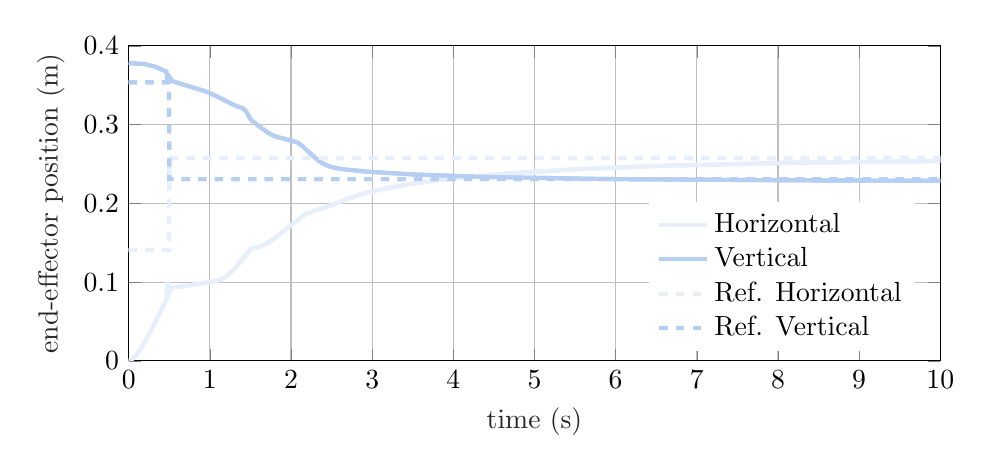
\begin{tikzpicture}

\begin{axis}[%
width=0.85\textwidth,
height=0.33\textwidth,
at={(0\textwidth,0\textwidth)},
scale only axis,
xmin=0,
xmax=10,
xlabel style={font=\color{white!15!black}},
xlabel={time (s)},
ymin=0,
ymax=0.4,
ylabel style={font=\color{white!15!black}},
ylabel={end-effector position (m)},
axis background/.style={fill=white},
xmajorgrids,
ymajorgrids,
legend style={at={(0.97,0.03)}, anchor=south east, legend cell align=left, align=left, draw=none}
]
\addplot [color=mycolor1, line width=1.5pt]
  table[row sep=crcr]{%
0	2.77612271712968e-05\\
0.0359999999999996	0.00166463670178274\\
0.0839999999999996	0.0062538502240912\\
0.144	0.0144972159183645\\
0.215999999999999	0.026948073810086\\
0.316000000000001	0.0469565619180514\\
0.464	0.0777105322504195\\
0.468	0.0819940250197355\\
0.476000000000001	0.0977350588157027\\
0.48	0.0975973855605901\\
0.488	0.0876065468541398\\
0.492000000000001	0.086925827234051\\
0.504	0.0938854354255643\\
0.52	0.0909708156376805\\
0.532	0.0933585410218818\\
0.556000000000001	0.0932999188591648\\
0.572000000000001	0.0933381343057125\\
0.648	0.094424008856139\\
1.072	0.101134047264006\\
1.176	0.105214897570557\\
1.292	0.115295252943604\\
1.4	0.128676835663995\\
1.5	0.141629094839667\\
1.556	0.143608303508916\\
1.628	0.145683094533913\\
1.72	0.149966567900119\\
1.8	0.156071549600348\\
2.176	0.186374826150482\\
2.3	0.190834715278784\\
2.436	0.195399193220851\\
2.856	0.211560030974312\\
3.144	0.21862101854655\\
3.524	0.225462652024973\\
4.028	0.232028207260921\\
4.688	0.238128976268008\\
5.536	0.243462857460786\\
6.64	0.247908897543834\\
8.148	0.251453230838147\\
10	0.253782095688482\\
};
\addlegendentry{Horizontal}

\addplot [color=mycolor2, line width=1.5pt]
  table[row sep=crcr]{%
0	0.377999995238071\\
0.199999999999999	0.376816401680257\\
0.324	0.37358316118865\\
0.456	0.367621520570324\\
0.464	0.36719406141942\\
0.468	0.365527834769907\\
0.476000000000001	0.357366290317353\\
0.48	0.357563159282824\\
0.488	0.362187915564183\\
0.492000000000001	0.362132309332786\\
0.504	0.357334014824138\\
0.52	0.357801845966438\\
0.532	0.355654127844451\\
0.576000000000001	0.353860760341448\\
0.635999999999999	0.351900964689856\\
0.952	0.342060969200135\\
1.108	0.334640296067828\\
1.308	0.324348552401471\\
1.408	0.320441385189158\\
1.436	0.317925801250738\\
1.46	0.314423528094856\\
1.492	0.308345106364522\\
1.528	0.304080807566127\\
1.604	0.298035022662487\\
1.708	0.290281708358089\\
1.752	0.28757051994603\\
1.824	0.284322455022322\\
1.92	0.28189213647407\\
2.084	0.277083330401922\\
2.144	0.272315419017479\\
2.332	0.254500133363212\\
2.428	0.248752968184506\\
2.492	0.246246912578648\\
2.628	0.243425473322391\\
2.924	0.240345215271432\\
3.492	0.236699956793988\\
4.392	0.233524109855862\\
5.892	0.230867077626547\\
8.344	0.229124962082716\\
10	0.228619850093684\\
};
\addlegendentry{Vertical}

\addplot [color=mycolor1, dashed, line width=1.5pt]
  table[row sep=crcr]{%
0	0.140599999999999\\
0.496	0.140599999999999\\
0.5	0.2576\\
10	0.2576\\
};
\addlegendentry{Ref. Horizontal}

\addplot [color=mycolor2, dashed, line width=1.5pt]
  table[row sep=crcr]{%
0	0.3537\\
0.496	0.3537\\
0.5	0.230700000000001\\
10	0.230700000000001\\
};
\addlegendentry{Ref. Vertical}

\addplot [color=mycolor1, line width=1.5pt, forget plot]
  table[row sep=crcr]{%
0	2.77612271712968e-05\\
0.0359999999999996	0.00166463670178274\\
0.0839999999999996	0.0062538502240912\\
0.144	0.0144972159183645\\
0.215999999999999	0.026948073810086\\
0.316000000000001	0.0469565619180514\\
0.464	0.0777105322504195\\
0.468	0.0819940250197355\\
0.476000000000001	0.0977350588157027\\
0.48	0.0975973855605901\\
0.488	0.0876065468541398\\
0.492000000000001	0.086925827234051\\
0.504	0.0938854354255643\\
0.52	0.0909708156376805\\
0.532	0.0933585410218818\\
0.556000000000001	0.0932999188591648\\
0.572000000000001	0.0933381343057125\\
0.648	0.094424008856139\\
1.072	0.101134047264006\\
1.176	0.105214897570557\\
1.292	0.115295252943604\\
1.4	0.128676835663995\\
1.5	0.141629094839667\\
1.556	0.143608303508916\\
1.628	0.145683094533913\\
1.72	0.149966567900119\\
1.8	0.156071549600348\\
2.176	0.186374826150482\\
2.3	0.190834715278784\\
2.436	0.195399193220851\\
2.856	0.211560030974312\\
3.144	0.21862101854655\\
3.524	0.225462652024973\\
4.028	0.232028207260921\\
4.688	0.238128976268008\\
5.536	0.243462857460786\\
6.64	0.247908897543834\\
8.148	0.251453230838147\\
10	0.253782095688482\\
};
\addplot [color=mycolor2, line width=1.5pt, forget plot]
  table[row sep=crcr]{%
0	0.377999995238071\\
0.199999999999999	0.376816401680257\\
0.324	0.37358316118865\\
0.456	0.367621520570324\\
0.464	0.36719406141942\\
0.468	0.365527834769907\\
0.476000000000001	0.357366290317353\\
0.48	0.357563159282824\\
0.488	0.362187915564183\\
0.492000000000001	0.362132309332786\\
0.504	0.357334014824138\\
0.52	0.357801845966438\\
0.532	0.355654127844451\\
0.576000000000001	0.353860760341448\\
0.635999999999999	0.351900964689856\\
0.952	0.342060969200135\\
1.108	0.334640296067828\\
1.308	0.324348552401471\\
1.408	0.320441385189158\\
1.436	0.317925801250738\\
1.46	0.314423528094856\\
1.492	0.308345106364522\\
1.528	0.304080807566127\\
1.604	0.298035022662487\\
1.708	0.290281708358089\\
1.752	0.28757051994603\\
1.824	0.284322455022322\\
1.92	0.28189213647407\\
2.084	0.277083330401922\\
2.144	0.272315419017479\\
2.332	0.254500133363212\\
2.428	0.248752968184506\\
2.492	0.246246912578648\\
2.628	0.243425473322391\\
2.924	0.240345215271432\\
3.492	0.236699956793988\\
4.392	0.233524109855862\\
5.892	0.230867077626547\\
8.344	0.229124962082716\\
10	0.228619850093684\\
};
\addplot [color=mycolor1, dashed, line width=1.5pt, forget plot]
  table[row sep=crcr]{%
0	0.140599999999999\\
0.496	0.140599999999999\\
0.5	0.2576\\
10	0.2576\\
};
\addplot [color=mycolor2, dashed, line width=1.5pt, forget plot]
  table[row sep=crcr]{%
0	0.3537\\
0.496	0.3537\\
0.5	0.230700000000001\\
10	0.230700000000001\\
};
\end{axis}

\begin{axis}[%
width=0.545\textwidth,
height=0.313\textwidth,
at={(-0.071\textwidth,-0.045\textwidth)},
scale only axis,
xmin=0,
xmax=1,
ymin=0,
ymax=1,
axis line style={draw=none},
ticks=none,
axis x line*=bottom,
axis y line*=left
]
\end{axis}
\end{tikzpicture}%

    \caption{\small The end-effector trajectories of the six-link soft manipulator, where $\{$\ldata{Matlab1}, \ldata{Matlab2}$\}$ denote the horizontal and vertical position, respectively. The setpoints assigned by the controller are indicated by the dashed lines. Note that at $t \approx 0.88$ (s), the point of contact, the controller switches setpoint. }
    \label{fig:C5:dellasantina_endeffector}
    \vspace{-3mm}
\end{figure}
%
\begin{figure}[!t]
    \centering
    %\vspace{-20mm}
    \includegraphics*[width=0.8\textwidth]{./pdf/thesis-figure-6-31.pdf}
    %% This file was created by matlab2tikz.
%
%The latest updates can be retrieved from
%  http://www.mathworks.com/matlabcentral/fileexchange/22022-matlab2tikz-matlab2tikz
%where you can also make suggestions and rate matlab2tikz.
%
\definecolor{mycolor1}{rgb}{0.06275,0.35686,0.84706}%
\definecolor{mycolor2}{rgb}{0.86667,0.21176,0.10980}%
\definecolor{mycolor3}{rgb}{0.18039,0.52157,0.25098}%
\definecolor{mycolor4}{rgb}{1.00000,0.61569,0.11765}%
\definecolor{mycolor5}{rgb}{0.29804,0.17255,0.57255}%
\definecolor{mycolor6}{rgb}{1.00000,0.39216,0.11765}%
%
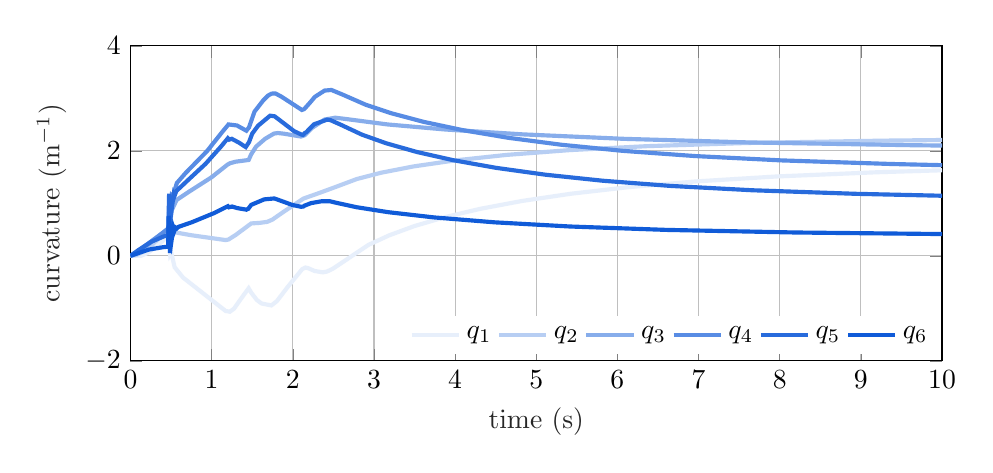
\begin{tikzpicture}

\begin{axis}[%
width=0.85\textwidth,
height=0.33\textwidth,
at={(0\textwidth,0\textwidth)},
scale only axis,
xmin=0,
xmax=10,
xlabel style={font=\color{white!15!black}},
xlabel={time (s)},
ymin=-2,
ymax=4,
ylabel style={font=\color{white!15!black}},
ylabel={curvature (m$^{-1}$)},
axis background/.style={fill=white},
xmajorgrids,
ymajorgrids,
legend style={at={(1,0.02)}, anchor=south east, legend columns=6, legend cell align=left, align=left, draw=none}
]
\addplot [color=mycolor1, line width=1.5pt]
  table[row sep=crcr]{%
0	2.36483362936468e-05\\
0.128	-4.25819815870199e-05\\
0.212	0.0556790499212383\\
0.327999999999999	0.186975922139752\\
0.472	0.387361233927445\\
0.488	0.0443283231030289\\
0.5	0.0829146935740628\\
0.544	-0.217152707197901\\
0.648	-0.413980890230992\\
1.172	-1.04940429645464\\
1.224	-1.06377117024523\\
1.276	-1.00544798479627\\
1.364	-0.811707499767255\\
1.456	-0.617287768432304\\
1.488	-0.701916150476235\\
1.556	-0.838426094017111\\
1.616	-0.907396677410501\\
1.736	-0.944261670542058\\
1.804	-0.862004485148759\\
1.936	-0.594406898056025\\
2.116	-0.252924225488682\\
2.156	-0.222305298736595\\
2.188	-0.233689696703799\\
2.268	-0.287449817315009\\
2.368	-0.313960033814064\\
2.42	-0.299871423111584\\
2.496	-0.242864173360999\\
2.932	0.208397183054636\\
3.188	0.390781992094489\\
3.496	0.565781002966242\\
3.868	0.734657355049801\\
4.308	0.895019647816286\\
4.824	1.04505480576187\\
5.428	1.18320984107613\\
6.136	1.30797745498677\\
6.972	1.41787706234173\\
7.964	1.51195799447709\\
9.2	1.59218802646173\\
10	1.62952637233137\\
};
\addlegendentry{$q_1$}

\addplot [color=mycolor2, line width=1.5pt]
  table[row sep=crcr]{%
0	-7.85080617422551e-05\\
0.0719999999999992	0.0152438876786007\\
0.16	0.0824963963381879\\
0.279999999999999	0.229411297954012\\
0.464	0.507517685642698\\
0.476000000000001	0.442358842131142\\
0.488	0.620526220451014\\
0.504	0.463898043070341\\
0.516	0.499473211949509\\
0.532	0.452569905103282\\
0.747999999999999	0.39295140311989\\
1.172	0.300596909461888\\
1.208	0.311736303268646\\
1.296	0.397286014394691\\
1.488	0.617580729136556\\
1.592	0.628029802859018\\
1.684	0.647284522375694\\
1.748	0.689462329688693\\
1.88	0.831627172243927\\
2.132	1.09133146966791\\
2.3	1.18285730152837\\
2.492	1.2913462549178\\
2.788	1.46275323747345\\
3.088	1.58296531395995\\
3.488	1.7031659140314\\
3.996	1.81706246223768\\
4.632	1.92223766938991\\
5.408	2.01341578152064\\
6.364	2.08894698554045\\
7.596	2.14924933781959\\
9.284	2.19427573492612\\
10	2.20607522455517\\
};
\addlegendentry{$q_2$}

\addplot [color=mycolor3, line width=1.5pt]
  table[row sep=crcr]{%
0	-0.000115662527289118\\
0.0519999999999996	0.0269540165565427\\
0.176	0.160694330517005\\
0.464	0.523182829435372\\
0.472	0.497400676905924\\
0.488	0.915526258335987\\
0.5	0.767959818111747\\
0.516	0.934864756096417\\
0.524000000000001	0.918685008217549\\
0.568	1.06356281175899\\
0.736000000000001	1.23627524970105\\
0.996	1.49318042652942\\
1.196	1.73772889401984\\
1.228	1.76442247587729\\
1.296	1.79331002099016\\
1.456	1.82608077376538\\
1.488	1.93592054969327\\
1.548	2.08089985638041\\
1.66	2.23012868887301\\
1.768	2.3285068337313\\
1.816	2.33904162413898\\
1.892	2.32614335713947\\
2.1	2.27239966374133\\
2.148	2.29755484336023\\
2.236	2.43538699969822\\
2.392	2.59647500084244\\
2.524	2.63063004989941\\
2.652	2.6067097738336\\
3.168	2.5024330508405\\
3.88	2.40613270725078\\
4.84	2.31301010569398\\
6.088	2.22807125426015\\
7.624	2.15980307682888\\
9.616	2.10745316243604\\
10	2.10042681665129\\
};
\addlegendentry{$q_3$}

\addplot [color=mycolor4, line width=1.5pt]
  table[row sep=crcr]{%
0	0.000151035756738693\\
0.0519999999999996	0.0461043707422739\\
0.404	0.445028700088937\\
0.468	0.519469225344928\\
0.48	1.02384926886379\\
0.492000000000001	0.814298948161623\\
0.508000000000001	1.13161900770105\\
0.516	1.11596234236197\\
0.572000000000001	1.38778163448256\\
0.68	1.57859956962357\\
0.944000000000001	1.9959898959421\\
1.136	2.369330908569\\
1.208	2.50294335008777\\
1.312	2.48276462213886\\
1.428	2.38306831600037\\
1.46	2.44532112041825\\
1.528	2.74568740101295\\
1.636	2.96119619500234\\
1.696	3.05281073208953\\
1.74	3.0903004575145\\
1.788	3.09119890298268\\
1.86	3.03155495796519\\
2.112	2.77840284577578\\
2.14	2.79397840967848\\
2.208	2.91033867446406\\
2.272	3.02805888072867\\
2.392	3.1475666656483\\
2.476	3.15918833341086\\
2.62	3.06685484012069\\
2.9	2.87695221670009\\
3.212	2.71647696623253\\
3.612	2.5518845216304\\
4.092	2.39466425238844\\
4.66	2.24710360208926\\
5.312	2.11528869757987\\
6.068	1.99953327923031\\
6.952	1.90086802083478\\
8.024	1.81762864310982\\
9.38	1.74920226662956\\
10	1.72696940349711\\
};
\addlegendentry{$q_4$}

\addplot [color=mycolor5, line width=1.5pt]
  table[row sep=crcr]{%
0	0.00127687703484369\\
0.0920000000000005	0.103566647754015\\
0.256	0.26745642692768\\
0.407999999999999	0.368827176958614\\
0.464	0.394829053784976\\
0.476000000000001	1.18379556138303\\
0.488	0.462793393751133\\
0.504	1.07599578189597\\
0.512	0.93824442957918\\
0.532	1.15920499451121\\
0.540000000000001	1.12882091957026\\
0.564	1.23212858035494\\
0.720000000000001	1.45866132674927\\
0.923999999999999	1.750573124951\\
1.112	2.0757681745642\\
1.2	2.23972742168971\\
1.216	2.21266461762795\\
1.248	2.22896601476036\\
1.336	2.15682876356869\\
1.42	2.07163048632857\\
1.46	2.16324467493075\\
1.5	2.32761818449978\\
1.572	2.47795375989802\\
1.72	2.66913570790783\\
1.748	2.66388665565618\\
1.776	2.65774005141227\\
2.016	2.37481145981238\\
2.108	2.30802136327647\\
2.128	2.30544930625548\\
2.148	2.34020580724893\\
2.168	2.35674706488961\\
2.2	2.41018031502332\\
2.264	2.5070296153121\\
2.424	2.59443445940502\\
2.464	2.58487043984969\\
2.588	2.49935486527589\\
2.852	2.30837697258491\\
3.152	2.14328838070271\\
3.532	1.97678524384419\\
3.976	1.8220350809767\\
4.504	1.67613212306702\\
5.116	1.54475302597869\\
5.82	1.43052335340367\\
6.652	1.33204329076605\\
7.664	1.24902151046343\\
8.936	1.18152440552507\\
10	1.14451846636578\\
};
\addlegendentry{$q_5$}

\addplot [color=mycolor6, line width=1.5pt]
  table[row sep=crcr]{%
0	0.00178900633679469\\
0.228	0.120314514661294\\
0.407999999999999	0.166501989702192\\
0.464	0.173710618311819\\
0.472	0.760824585947576\\
0.476000000000001	0.701883551946707\\
0.488	0.0518527806458629\\
0.5	0.557040009999261\\
0.512	0.3561303103128\\
0.528	0.531027852147922\\
0.540000000000001	0.471774053062605\\
0.556000000000001	0.540074059700961\\
0.572000000000001	0.524549737481115\\
0.592000000000001	0.552466477967732\\
0.756	0.640092367045868\\
1.024	0.810360490998393\\
1.2	0.945920226932708\\
1.212	0.92445100085674\\
1.252	0.9391254011674\\
1.316	0.909316621905269\\
1.428	0.879512480250003\\
1.452	0.896328270713198\\
1.488	0.971293512576786\\
1.648	1.07575178303653\\
1.772	1.0931754504335\\
1.812	1.07190587618337\\
1.996	0.968499720807907\\
2.1	0.935274971566722\\
2.128	0.937897610214575\\
2.144	0.95568302931178\\
2.172	0.972307726877974\\
2.224	1.00360027115423\\
2.284	1.02050416936917\\
2.36	1.04048370155465\\
2.456	1.04010259441693\\
2.524	1.01466708236405\\
2.784	0.926875830011378\\
3.176	0.831594341546401\\
3.744	0.731367635050987\\
4.488	0.638251274953785\\
5.42	0.558640715136692\\
6.608	0.494052577730045\\
8.2	0.444648508311996\\
10	0.415216786709284\\
};
\addlegendentry{$q_6$}

\end{axis}

\begin{axis}[%
width=0.513\textwidth,
height=0.295\textwidth,
at={(-0.067\textwidth,-0.043\textwidth)},
scale only axis,
xmin=0,
xmax=1,
ymin=0,
ymax=1,
axis line style={draw=none},
ticks=none,
axis x line*=bottom,
axis y line*=left
]
\end{axis}
\end{tikzpicture}%

    \caption{\small State evolutions of the six-link soft manipulator, where the states represent the planar curvature of each individual soft link. }
    \label{fig:C5:dellasantina_states}
    \vspace{-3mm}
\end{figure}
%
\begin{figure}[!t]
    \centering
    %\vspace{-20mm}
    \includegraphics*[width=0.8\textwidth]{./pdf/thesis-figure-6-32.pdf}
    %% This file was created by matlab2tikz.
%
%The latest updates can be retrieved from
%  http://www.mathworks.com/matlabcentral/fileexchange/22022-matlab2tikz-matlab2tikz
%where you can also make suggestions and rate matlab2tikz.
%
\definecolor{mycolor1}{rgb}{0.06275,0.35686,0.84706}%
\definecolor{mycolor2}{rgb}{0.86667,0.21176,0.10980}%
\definecolor{mycolor3}{rgb}{0.18039,0.52157,0.25098}%
\definecolor{mycolor4}{rgb}{1.00000,0.61569,0.11765}%
\definecolor{mycolor5}{rgb}{0.29804,0.17255,0.57255}%
\definecolor{mycolor6}{rgb}{1.00000,0.39216,0.11765}%
%
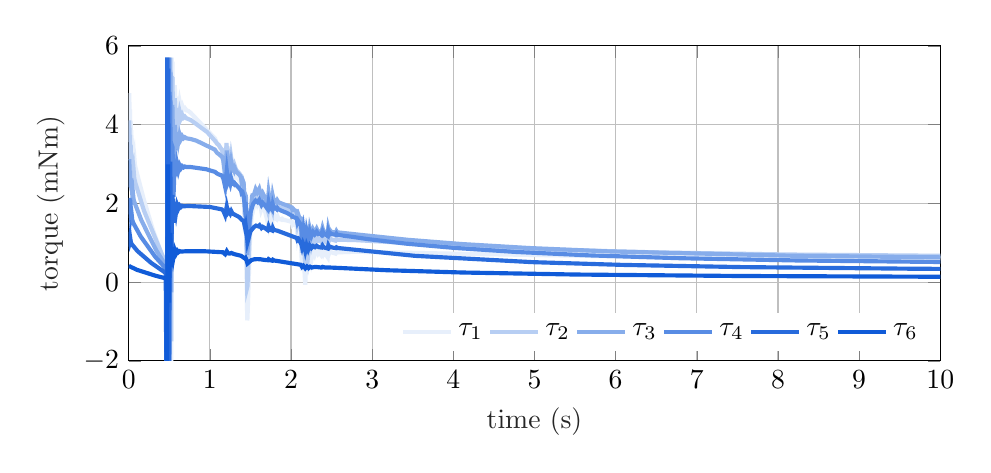
\begin{tikzpicture}

\begin{axis}[%
width=0.85\textwidth,
height=0.33\textwidth,
at={(0\textwidth,0\textwidth)},
scale only axis,
unbounded coords=jump,
xmin=0,
xmax=10,
xlabel style={font=\color{white!15!black}},
xlabel={time (s)},
ymin=-2,
ymax=6,
ylabel style={font=\color{white!15!black}},
ylabel={torque (mNm)},
axis background/.style={fill=white},
xmajorgrids,
ymajorgrids,
legend style={at={(0.99,0.03)}, anchor=south east, legend columns=6, legend cell align=left, align=left, draw=none}
]
\addplot [color=mycolor1, line width=1.5pt]
  table[row sep=crcr]{%
0	3.55592103167417\\
0.00399999999999956	3.63254838023404\\
0.00799999999999912	4.79703595073799\\
0.0120000000000005	3.64255818119174\\
0.016	4.38254542964753\\
0.0199999999999996	3.70856397082569\\
0.0239999999999991	4.09907806553181\\
0.0280000000000005	3.62350679292482\\
0.032	3.85465145654794\\
0.0359999999999996	3.50196782262192\\
0.0399999999999991	3.64900594863472\\
0.0440000000000005	3.38078423686617\\
0.048	3.47749674249152\\
0.0519999999999996	3.26863753698384\\
0.0559999999999992	3.33266744563688\\
0.0600000000000005	3.1662880001105\\
0.0640000000000001	3.20792853910502\\
0.0679999999999996	3.07255170607861\\
0.0719999999999992	3.09826228002341\\
0.0760000000000005	2.98595430812925\\
0.0839999999999996	2.90516272967436\\
0.183999999999999	2.11276455895664\\
0.295999999999999	1.34374472879786\\
0.436	0.538210024987633\\
0.464	0.40952825862988\\
0.464054459894024	-2.69999999999999\\
nan	nan\\
0.477259828621811	-2.69999999999999\\
0.477259828621811	-2.69999999999999\\
nan	nan\\
0.474080226859831	-2.69999999999999\\
0.474216778575903	5.69999999999999\\
nan	nan\\
0.480785903808583	5.7\\
0.480785903808583	5.7\\
nan	nan\\
0.480634955662824	5.7\\
0.480931049836688	-2.70000000000002\\
nan	nan\\
0.486537600776424	-2.7\\
0.486782430039042	5.7\\
nan	nan\\
0.501456359120251	5.7\\
0.501456359120251	5.7\\
nan	nan\\
0.493633867027597	5.7\\
0.494101375752411	-2.7\\
nan	nan\\
0.499919546716594	-2.7\\
0.501804991016156	5.7\\
nan	nan\\
0.517108386117986	5.7\\
0.524037003026612	-2.7\\
0.531784391608866	5.7\\
nan	nan\\
0.540000000000001	5.59957845921779\\
0.552	2.55239609909956\\
0.568	5.00282992229886\\
0.584	3.99185645027749\\
0.596	4.70239906018891\\
0.603999999999999	4.54733571002356\\
0.612	4.3008529128676\\
0.619999999999999	4.44516882751612\\
0.628	4.56876135182694\\
0.644	4.38719285825855\\
0.66	4.47757991568239\\
0.676	4.38776975807044\\
0.692	4.41678262512577\\
0.712	4.36011953483898\\
0.736000000000001	4.34385035818736\\
0.76	4.30558251488896\\
1.064	3.64697814890311\\
1.088	3.51735077825992\\
1.108	3.4768948017728\\
1.144	3.34170815439209\\
1.156	3.31216281424314\\
1.172	2.89245875952029\\
1.188	2.54637840209652\\
1.192	2.57896896548633\\
1.204	3.4971096195561\\
1.216	3.16458656666485\\
1.224	2.83728571214052\\
1.236	3.00011411250631\\
1.252	2.70962583855029\\
1.264	3.03093449273775\\
1.28	2.76920997328179\\
1.288	2.81114365439141\\
1.3	2.71503227101871\\
1.308	2.80194190966736\\
1.324	2.68839229641105\\
1.36	2.59755655392518\\
1.384	2.48837590878836\\
1.392	2.30330959444324\\
1.404	2.38628470126293\\
1.416	2.29038175816832\\
1.432	1.23733807845379\\
1.44	1.73602153341136\\
1.444	1.69941096687715\\
1.46	-0.970710808625446\\
1.464	-0.909364035127215\\
1.496	1.15831295229913\\
1.524	1.90004535037176\\
1.536	1.85791925487358\\
1.552	2.03731062176827\\
1.564	2.13529142371901\\
1.584	1.98966373354341\\
1.608	2.13232055471224\\
1.624	1.92336628542107\\
1.632	1.83033666576196\\
1.652	1.94187920970976\\
1.664	1.8548014943986\\
1.676	1.83329769342294\\
1.712	1.52078454972759\\
1.724	1.92293900015338\\
1.74	1.60865370758907\\
1.748	1.66292279881596\\
1.768	1.51520617238823\\
1.776	1.78328034642033\\
1.788	1.63249054165978\\
1.8	1.67215514962973\\
1.812	1.60969935983956\\
1.824	1.59204048466297\\
1.836	1.65621157387206\\
1.844	1.61168585067016\\
1.884	1.58423487947198\\
1.892	1.60295629569636\\
1.904	1.58431589607896\\
2.008	1.533809702481\\
2.016	1.4583189086272\\
2.028	1.48905829480673\\
2.04	1.45601693749202\\
2.068	1.43772389588811\\
2.08	1.1677776588766\\
2.092	1.29484960099783\\
2.104	1.1907054707069\\
2.12	1.18352029061195\\
2.136	0.290373402146113\\
2.152	0.881498318700418\\
2.168	0.181808952726232\\
2.176	-0.0654007747944476\\
2.192	0.779916394430728\\
2.212	0.280240072003291\\
2.22	0.474467321881537\\
2.232	0.842335940105684\\
2.252	0.585026804209917\\
2.264	0.745712598704857\\
2.272	0.818898070528773\\
2.292	0.702674183844021\\
2.316	0.856271364996546\\
2.336	0.721944793814567\\
2.348	0.750080297720984\\
2.372	0.683825559890961\\
2.376	0.700774134446222\\
2.388	0.878468208509874\\
2.404	0.720973548909624\\
2.412	0.75118006623955\\
2.452	0.630241787713377\\
2.46	0.854149680439933\\
2.472	0.749357009045557\\
2.48	0.796736061211941\\
2.492	0.758818264618059\\
2.548	0.723723225172868\\
2.56	0.776980858147279\\
2.568	0.752091663443366\\
2.624	0.758364540425111\\
2.784	0.769680585252408\\
3.068	0.761011005954373\\
4.136	0.716792420748183\\
6.036	0.652993437324465\\
8.256	0.614421294268528\\
10	0.601787409397712\\
};
\addlegendentry{$\tau_1$}

\addplot [color=mycolor2, line width=1.5pt]
  table[row sep=crcr]{%
0	3.08882591384591\\
0.00399999999999956	3.14928998567576\\
0.00799999999999912	4.10558208246037\\
0.0120000000000005	3.14762457712799\\
0.016	3.73712936585095\\
0.0199999999999996	3.1884699265051\\
0.0239999999999991	3.49129891754317\\
0.0280000000000005	3.10965749230231\\
0.032	3.28508701066692\\
0.0359999999999996	3.00478297298584\\
0.0399999999999991	3.11413494161282\\
0.0440000000000005	2.90226923511392\\
0.048	2.97256670356227\\
0.0519999999999996	2.80819077630425\\
0.0559999999999992	2.85336331359795\\
0.0600000000000005	2.72264763160815\\
0.0640000000000001	2.75074126289659\\
0.0679999999999996	2.64440788555003\\
0.0760000000000005	2.57213057773123\\
0.0839999999999996	2.50465622809443\\
0.188000000000001	1.81345253096712\\
0.464	0.432220113112542\\
0.464075972610202	-2.69999999999999\\
nan	nan\\
0.477685777050405	-2.69999999999999\\
0.477685777050405	-2.7\\
nan	nan\\
0.474052693672057	-2.70000000000002\\
0.474234253940065	5.7\\
nan	nan\\
0.480807654923511	5.69999999999999\\
0.480807654923511	5.7\\
nan	nan\\
0.480735348238426	5.7\\
0.481185431714293	-2.7\\
nan	nan\\
0.486340978723685	-2.69999999999999\\
0.486715329506447	5.7\\
nan	nan\\
0.49943975774581	5.7\\
0.49943975774581	5.7\\
nan	nan\\
0.493456089894831	5.7\\
0.494108518835883	-2.7\\
nan	nan\\
0.499783212693439	-2.7\\
0.502121096888027	5.7\\
nan	nan\\
0.516740272002435	5.7\\
0.524000000000001	-1.50300764900957\\
0.532	5.23594592379653\\
nan	nan\\
0.540000000000001	5.20256998869543\\
0.552	2.65435909697568\\
0.568	4.67172398061227\\
0.584	3.82042633951941\\
0.596	4.42152521112568\\
0.603999999999999	4.29280950236743\\
0.612	4.08590486610147\\
0.619999999999999	4.20847120513033\\
0.628	4.31780520043572\\
0.644	4.16678873362386\\
0.66	4.24773019374899\\
0.676	4.17454100737093\\
0.692	4.20285575174431\\
0.712	4.15873035966959\\
0.763999999999999	4.11617151487747\\
0.968	3.80767354171773\\
1.072	3.56654259455107\\
1.088	3.51782242210752\\
1.108	3.48682129918518\\
1.132	3.40512237457358\\
1.148	3.37063850208853\\
1.164	3.23778788045077\\
1.188	2.7282140426765\\
1.196	2.90011860713025\\
1.204	3.53159379904974\\
1.216	3.25211202708226\\
1.224	2.9781085675558\\
1.236	3.11571088208201\\
1.252	2.87611019653523\\
1.264	3.1447524382783\\
1.28	2.92440130660698\\
1.288	2.95889490507096\\
1.3	2.87798287712077\\
1.308	2.94932994112599\\
1.324	2.85221435205499\\
1.364	2.76038622514453\\
1.384	2.67470081899613\\
1.392	2.52259435016537\\
1.404	2.58716545916438\\
1.416	2.50632385726953\\
1.432	1.66318730880862\\
1.44	2.05696343152172\\
1.444	2.02804014684736\\
1.46	-0.130145609837323\\
1.464	-0.0971019975629037\\
1.496	1.53819415036543\\
1.524	2.13986057168803\\
1.536	2.11392583259282\\
1.552	2.25398273534014\\
1.564	2.33897327714091\\
1.584	2.22388099480962\\
1.608	2.34469825722668\\
1.62	2.23046938435915\\
1.636	2.08699506743418\\
1.652	2.18559518511387\\
1.664	2.1153041398862\\
1.676	2.09993135694196\\
1.712	1.83675208380108\\
1.724	2.18407573462462\\
1.74	1.91137747394036\\
1.748	1.95860093199546\\
1.768	1.83231986120814\\
1.776	2.06695098424608\\
1.788	1.92890506989072\\
1.796	1.96557639599034\\
1.812	1.90819567689202\\
1.824	1.89174232699321\\
1.836	1.94885822059981\\
1.844	1.90575532074532\\
1.944	1.85249947250846\\
1.976	1.82404002546466\\
2.008	1.80690687802043\\
2.016	1.73708937303975\\
2.028	1.76360310244602\\
2.04	1.7319024568019\\
2.068	1.71084270896318\\
2.08	1.47658933339089\\
2.092	1.58358976191782\\
2.104	1.49277045587072\\
2.12	1.48409989096881\\
2.136	0.742061149236728\\
2.152	1.22477089806038\\
2.168	0.640549425638516\\
2.176	0.426907691924836\\
2.192	1.12507247984653\\
2.212	0.696748726288968\\
2.22	0.852515789969788\\
2.232	1.16787948507359\\
2.252	0.944585746451855\\
2.26	1.01563845006414\\
2.272	1.14342626006575\\
2.292	1.04047553259641\\
2.316	1.17467545593562\\
2.336	1.05627645276799\\
2.352	1.0788651843666\\
2.372	1.02201294929818\\
2.388	1.1975880844752\\
2.404	1.05493736652228\\
2.412	1.08241701398474\\
2.452	0.974435163185541\\
2.46	1.18371401486666\\
2.472	1.07889767994823\\
2.48	1.12546755861251\\
2.492	1.08772838830329\\
2.548	1.05261830408326\\
2.56	1.10510458907238\\
2.568	1.07695503523722\\
2.644	1.07315264223144\\
2.796	1.06563207669559\\
4.108	0.9140831053688\\
5.216	0.824855959781681\\
6.548	0.752107738462891\\
8.152	0.700313807548868\\
10	0.668902803464178\\
};
\addlegendentry{$\tau_2$}

\addplot [color=mycolor3, line width=1.5pt]
  table[row sep=crcr]{%
0	2.41685508414774\\
0.00399999999999956	2.45506794860088\\
0.00799999999999912	3.12066776926352\\
0.0120000000000005	2.43915215445037\\
0.016	2.82815246119562\\
0.0199999999999996	2.45095840431358\\
0.0239999999999991	2.64180691937338\\
0.0280000000000005	2.38502950364645\\
0.032	2.49145478577328\\
0.0359999999999996	2.30535468607424\\
0.0399999999999991	2.36919907865073\\
0.0440000000000005	2.22956423402803\\
0.048	2.26872467683656\\
0.0519999999999996	2.1607137623417\\
0.0559999999999992	2.18422077752016\\
0.0600000000000005	2.09830611133566\\
0.0679999999999996	2.0412086605347\\
0.156000000000001	1.56961210361156\\
0.34	0.804251016017163\\
0.464	0.400231985063641\\
0.464123816293617	-2.7\\
nan	nan\\
0.478102830512093	-2.7\\
0.478102830512093	-2.70000000000001\\
nan	nan\\
0.474009008599781	-2.70000000000001\\
0.474296849229034	5.7\\
nan	nan\\
0.480801663375965	5.7\\
0.480801663375965	5.7\\
nan	nan\\
0.480923827383677	5.7\\
0.481858995083666	-2.7\\
nan	nan\\
0.485795361461639	-2.7\\
0.486579555853684	5.7\\
nan	nan\\
0.496306288490127	5.7\\
0.496306288490127	5.7\\
nan	nan\\
0.49305355905582	5.7\\
0.494175480230954	-2.7\\
nan	nan\\
0.499463446211864	-2.7\\
0.502899787053856	5.7\\
nan	nan\\
0.516	5.32763810983003\\
0.524000000000001	-0.260924617587516\\
0.536	4.49692843706794\\
0.540000000000001	4.40975964633088\\
0.552	2.53172565363966\\
0.568	3.98882202639224\\
0.584	3.35662640780752\\
0.596	3.80887204685095\\
0.612	3.56312462464394\\
0.619999999999999	3.65638757111643\\
0.628	3.74428067967481\\
0.644	3.63523808371669\\
0.66	3.70215674875605\\
0.676	3.6516564568878\\
0.692	3.67830686867785\\
0.712	3.65104174468962\\
0.768000000000001	3.63119020929801\\
0.827999999999999	3.59551614697892\\
0.852	3.57278689579771\\
1.06	3.36580476340074\\
1.088	3.28223524692156\\
1.112	3.24872652287485\\
1.132	3.21023852935942\\
1.148	3.19010329254511\\
1.164	3.10530639102579\\
1.188	2.7344502876824\\
1.196	2.8584635555167\\
1.208	3.33997898358183\\
1.224	2.92196554423993\\
1.236	3.02319190295968\\
1.252	2.84958690863873\\
1.264	3.04393024927764\\
1.28	2.87777510403025\\
1.288	2.90077190754815\\
1.3	2.83841322326638\\
1.308	2.88727098071057\\
1.324	2.8099550842079\\
1.372	2.70514807398647\\
1.384	2.65370184730681\\
1.392	2.54372061849409\\
1.404	2.58259305411532\\
1.416	2.51971249989244\\
1.432	1.9437333148647\\
1.44	2.20366089085423\\
1.444	2.18357852524359\\
1.46	0.691932631387095\\
1.52	2.1836388777436\\
1.528	2.20959087678756\\
1.544	2.22038833528914\\
1.564	2.35469908788803\\
1.584	2.2788756687799\\
1.608	2.3694780731034\\
1.636	2.17448988537943\\
1.652	2.25425433389236\\
1.664	2.20588401754412\\
1.684	2.12086653230133\\
1.712	2.00289964851056\\
1.724	2.26731074409295\\
1.74	2.05604479319024\\
1.748	2.09190310437803\\
1.768	1.99510809983815\\
1.776	2.17674891214962\\
1.788	2.06080811168129\\
1.796	2.08995992568124\\
1.824	2.02547330009359\\
1.832	2.07039126145417\\
1.844	2.02998646222879\\
1.884	1.99500233309914\\
1.948	1.94847400252181\\
2.008	1.8981610219756\\
2.016	1.83910118992921\\
2.028	1.85790417994803\\
2.04	1.828963534494\\
2.068	1.80404541716537\\
2.08	1.62357652464035\\
2.092	1.70097080863033\\
2.104	1.62977242445142\\
2.12	1.61897961479869\\
2.136	1.08588088022485\\
2.152	1.42247274300118\\
2.168	0.999800336584499\\
2.176	0.838199888108555\\
2.192	1.33430698070659\\
2.208	1.07079287513019\\
2.212	1.01310629135317\\
2.22	1.11889096196495\\
2.232	1.35542998302682\\
2.252	1.18522291559611\\
2.272	1.33266555950187\\
2.292	1.25208174504986\\
2.316	1.35523857091436\\
2.336	1.26302735903086\\
2.352	1.28025930678858\\
2.372	1.23550847585997\\
2.388	1.37566257966575\\
2.404	1.26040484342617\\
2.412	1.28242926217447\\
2.452	1.19601446451433\\
2.46	1.3704371520491\\
2.472	1.27530046432309\\
2.48	1.31607515159762\\
2.492	1.28163929494469\\
2.552	1.25387406011493\\
2.56	1.29283293223646\\
2.568	1.26406789373531\\
2.648	1.24683499834897\\
2.84	1.20342477282491\\
3.44	1.07397746868753\\
4.1	0.966974514573799\\
4.94	0.864630105337429\\
5.916	0.779657632686462\\
8.132	0.67152214370447\\
10	0.628775963508815\\
};
\addlegendentry{$\tau_3$}

\addplot [color=mycolor4, line width=1.5pt]
  table[row sep=crcr]{%
0	1.74488425444958\\
0.00799999999999912	2.1345379180076\\
0.0120000000000005	1.73308040644875\\
0.016	1.93642592300727\\
0.0199999999999996	1.72357665843376\\
0.0239999999999991	1.81654440303483\\
0.0280000000000005	1.67471972429695\\
0.032	1.72309539189277\\
0.0359999999999996	1.62138486844469\\
0.0399999999999991	1.64807604608748\\
0.0440000000000005	1.57196406259688\\
0.0519999999999996	1.52734802877219\\
0.0600000000000005	1.48684163032797\\
0.148	1.15781563764927\\
0.327999999999999	0.639842223727014\\
0.464	0.329428962745833\\
0.46423738576561	-2.7\\
nan	nan\\
0.477928049618535	-2.7\\
0.477928049618535	-2.7\\
nan	nan\\
0.473911174397481	-2.7\\
0.474471107212661	5.7\\
nan	nan\\
0.480699992240746	5.7\\
0.480699992240746	5.7\\
nan	nan\\
0.481307372856595	5.7\\
0.484	-1.33547198570412\\
0.486236237451047	5.7\\
nan	nan\\
0.492280918967687	5.7\\
0.492280918967687	5.7\\
nan	nan\\
0.492102577958452	5.7\\
0.494468899964295	-2.7\\
nan	nan\\
0.49869615632061	-2.7\\
0.504	4.82835649589249\\
0.508000000000001	4.33314361896304\\
0.512	4.61381644155138\\
0.524000000000001	0.525826344548825\\
0.536	3.4465681125179\\
0.540000000000001	3.42080545115578\\
0.552	2.16843610458251\\
0.568	3.11483822818449\\
0.584	2.68956616726378\\
0.596	2.99792923978808\\
0.612	2.83529172177562\\
0.628	2.9640259124193\\
0.644	2.89315052470338\\
0.66	2.94340559843855\\
0.676	2.91250749985002\\
0.692	2.93477031146247\\
0.712	2.92077450233804\\
0.76	2.92320938544175\\
0.956	2.8654926708489\\
1.012	2.82953948670139\\
1.064	2.79879038646327\\
1.088	2.75653282444066\\
1.116	2.72978051763649\\
1.148	2.70791478752083\\
1.168	2.61651619422059\\
1.188	2.42500538750036\\
1.2	2.67912206102017\\
1.208	2.83005204671084\\
1.224	2.54668470469118\\
1.236	2.61182912804049\\
1.252	2.5005522370316\\
1.264	2.62264757254513\\
1.28	2.51030577217223\\
1.3	2.47891809735571\\
1.308	2.50690644572856\\
1.36	2.38578618978351\\
1.384	2.32287837499713\\
1.392	2.25263424179527\\
1.404	2.26970364328669\\
1.42	2.14900719999903\\
1.432	1.88814085500506\\
1.44	2.03107886137582\\
1.452	1.63430697425891\\
1.464	1.11990112801936\\
1.5	1.76554965684502\\
1.532	1.98188489619058\\
1.556	2.04749407063098\\
1.564	2.07150574504916\\
1.588	2.02955847572925\\
1.608	2.08812390518399\\
1.624	2.01078802662129\\
1.636	1.95752321488377\\
1.652	2.0141915275679\\
1.664	1.98557065481542\\
1.684	1.93214178926659\\
1.712	1.85590483506299\\
1.724	2.03101705657577\\
1.74	1.88630927984295\\
1.748	1.90983955709277\\
1.768	1.84393401569088\\
1.776	1.96684095158987\\
1.788	1.87957900826552\\
1.796	1.89984954072712\\
1.824	1.84876129639981\\
1.832	1.87991136193491\\
1.848	1.84647862094785\\
1.884	1.81065820071064\\
1.948	1.75841805353229\\
2.012	1.68431902105758\\
2.016	1.66072286807283\\
2.068	1.62326125579582\\
2.08	1.50024942221386\\
2.092	1.54855492603816\\
2.108	1.49838497155128\\
2.124	1.42530689134086\\
2.136	1.15590033915267\\
2.152	1.35576724769406\\
2.168	1.09025773089387\\
2.176	0.983525038536198\\
2.192	1.28595801928764\\
2.208	1.11508661799438\\
2.212	1.0749554429889\\
2.232	1.2895672958875\\
2.252	1.17548542169765\\
2.272	1.26999867624355\\
2.292	1.21419590775009\\
2.316	1.28296592185301\\
2.336	1.21968473145102\\
2.356	1.22516423114303\\
2.372	1.19965149231855\\
2.388	1.29729257019173\\
2.404	1.21515380334358\\
2.412	1.23050656703959\\
2.452	1.16905826069705\\
2.46	1.29664117876959\\
2.472	1.22048635481504\\
2.48	1.25176825647607\\
2.492	1.22399798182327\\
2.552	1.19846547301956\\
2.56	1.22836228359836\\
2.568	1.20308422398232\\
2.66	1.17432575557779\\
2.74	1.15411793837066\\
2.944	1.09190740132568\\
3.416	0.976939135425656\\
4.008	0.869011123978456\\
4.768	0.766097114362436\\
5.68	0.678319046560182\\
6.792	0.606565888329884\\
8.228	0.549685408029562\\
10	0.510474831774392\\
};
\addlegendentry{$\tau_4$}

\addplot [color=mycolor5, line width=1.5pt]
  table[row sep=crcr]{%
0	1.07291342475141\\
0.00799999999999912	1.20099334176266\\
0.0120000000000005	1.04212035085925\\
0.016	1.10701833058172\\
0.0199999999999996	1.02501883419285\\
0.0239999999999991	1.05061180619694\\
0.0280000000000005	0.996220399429863\\
0.0359999999999996	0.967664552454513\\
0.108000000000001	0.788276725745485\\
0.276	0.4883759280962\\
0.456	0.232209004204083\\
0.464637444529066	-2.7\\
nan	nan\\
0.475744351220866	-2.7\\
0.475744351220866	-2.7\\
nan	nan\\
0.473477923203804	-2.7\\
0.475143468176567	5.7\\
nan	nan\\
0.488	5.41996898121252\\
0.495855702525418	-2.7\\
nan	nan\\
0.496226934818196	-2.7\\
0.512	3.05968366515948\\
0.524000000000001	0.719607331153364\\
0.540000000000001	2.21416844119854\\
0.552	1.5087106831827\\
0.568	2.02497317105761\\
0.584	1.78293854018925\\
0.596	1.95959851456574\\
0.612	1.86827354578372\\
0.628	1.94462665493239\\
0.644	1.90537868335381\\
0.66	1.93633721884244\\
0.68	1.9231759047217\\
0.728	1.93388893899614\\
1.004	1.90700638176477\\
1.072	1.87808952295437\\
1.148	1.84596914924787\\
1.168	1.80317334716019\\
1.188	1.70139754543001\\
1.2	1.83131488812027\\
1.208	1.92233863494799\\
1.224	1.76425322411756\\
1.236	1.79819662877474\\
1.252	1.73967131337232\\
1.264	1.80164902341095\\
1.28	1.73918982726932\\
1.3	1.71882824941227\\
1.364	1.64860590483207\\
1.388	1.59203347728283\\
1.396	1.57637947483663\\
1.416	1.55494056475918\\
1.432	1.39836737959585\\
1.44	1.45840970584933\\
1.452	1.27363223240979\\
1.464	1.01504361302178\\
1.5	1.2878495889939\\
1.54	1.39212555285872\\
1.568	1.43395314279196\\
1.596	1.41493174995638\\
1.612	1.44382581285273\\
1.636	1.37145776859299\\
1.652	1.40329051146743\\
1.664	1.38948638583507\\
1.684	1.36189272453193\\
1.712	1.32122621089731\\
1.724	1.41411287831039\\
1.74	1.33366485477038\\
1.768	1.30933383838071\\
1.776	1.37636081643223\\
1.788	1.3232828716129\\
1.828	1.3083404980111\\
2.072	1.11941695049967\\
2.08	1.06818770700392\\
2.092	1.09256900394254\\
2.128	0.958063316232943\\
2.136	0.888685404891332\\
2.148	0.983235285622964\\
2.164	0.905416463208685\\
2.176	0.789941226362728\\
2.192	0.936898101145857\\
2.208	0.846421187891773\\
2.212	0.82361575346405\\
2.232	0.931260873928258\\
2.252	0.868553225782374\\
2.272	0.916903553487996\\
2.296	0.887126277809369\\
2.316	0.921590325056167\\
2.34	0.887084408910216\\
2.376	0.877368803558531\\
2.388	0.928361779572393\\
2.404	0.880785680108799\\
2.452	0.853578030200779\\
2.46	0.928968165384484\\
2.472	0.880240012800977\\
2.48	0.899573762326932\\
2.516	0.874549765474553\\
2.552	0.863878653094648\\
2.56	0.882352461204979\\
2.572	0.866945390021039\\
3.528	0.666657704232458\\
4.972	0.506971711060572\\
6.084	0.436755681702087\\
7.544	0.381214778811009\\
9.612	0.340597660278286\\
10	0.335753532338726\\
};
\addlegendentry{$\tau_5$}

\addplot [color=mycolor6, line width=1.5pt]
  table[row sep=crcr]{%
0	0.420112134634961\\
0.0120000000000005	0.399158152810665\\
0.103999999999999	0.310133444060813\\
0.327999999999999	0.162934854350286\\
0.464	0.0919338787080886\\
0.467848125828533	-2.7\\
nan	nan\\
0.468217212242033	-2.7\\
0.484	2.99107909270009\\
0.496	-0.517911782640407\\
0.512	1.24598777664191\\
0.524000000000001	0.383340220731395\\
0.540000000000001	0.8902718889741\\
0.552	0.631907049623024\\
0.568	0.81587091861458\\
0.584	0.726414184154693\\
0.6	0.791163201594852\\
0.612	0.758191376849309\\
0.628	0.786995629800884\\
0.648	0.774971059810555\\
0.699999999999999	0.783094076622264\\
0.928000000000001	0.784083035309012\\
1.16	0.757445297183489\\
1.188	0.70798843026787\\
1.208	0.785651668758357\\
1.224	0.728907771174493\\
1.248	0.724997798601423\\
1.264	0.740843900801911\\
1.3	0.710528486044826\\
1.384	0.668521694221804\\
1.432	0.598486327665666\\
1.44	0.614602114337398\\
1.452	0.558094763037399\\
1.464	0.473006645566738\\
1.512	0.559255338232676\\
1.548	0.578885050676915\\
1.584	0.583717977614794\\
1.624	0.579754841277904\\
1.644	0.571965014168253\\
1.688	0.559400298111337\\
1.716	0.555892577800629\\
1.724	0.581722168840786\\
1.744	0.555140124496029\\
1.768	0.544177941541674\\
1.776	0.567661371187787\\
1.792	0.54885052972387\\
2.12	0.440037491012793\\
2.136	0.385208332118669\\
2.152	0.414062944272104\\
2.176	0.348869334296502\\
2.196	0.394928672610337\\
2.216	0.35558742438826\\
2.236	0.390711823649861\\
2.256	0.368989248880879\\
2.28	0.380995583252902\\
2.312	0.384054136672738\\
2.376	0.368893070812099\\
2.388	0.387261496992272\\
2.42	0.369269175071063\\
2.456	0.372058312818847\\
2.624	0.356217731313182\\
3.188	0.300817364517256\\
4.116	0.243280677210864\\
5.508	0.192150278507043\\
7.524	0.155081066900527\\
10	0.135636251316823\\
};
\addlegendentry{$\tau_6$}

\end{axis}

\begin{axis}[%
width=0.513\textwidth,
height=0.295\textwidth,
at={(-0.067\textwidth,-0.043\textwidth)},
scale only axis,
xmin=0,
xmax=1,
ymin=0,
ymax=1,
axis line style={draw=none},
ticks=none,
axis x line*=bottom,
axis y line*=left
]
\end{axis}
\end{tikzpicture}%

    \caption{\small The control inputs $\tauB$ in (\si{\milli \newton \meter}) produced by the control law in \eqref{eq:C5:dellasantina_controller} exhibit a significant peak at the point of contact. This is due to two factors: $(i)$ the sudden change of setpoint and $(ii)$ the switch in control strategy to accommodate for compliance.}
    \label{fig:C5:dellasantina_input}
    %\vspace{-3mm}
\end{figure}
\clearpage
}

When comparing the experimental results reported by Della Santina et al. \cite{DellaSantina2020Jan} and the numerical simulations produced by \texttt{Sorotoki}, we observe similar deformation characteristics in both systems. Most notably, the numerical implementation of the impedance Cartesian stiffness controller also follows the inclined surface until the setpoint is reached. These similarities highlight the reliability of \texttt{Sorotoki} in accurately reflecting true soft robotic systems, even in closed-loop scenarios. 

\subsection[Contact robust shape sensing of elastomer soft actuator]{Contact robust shape sensing of elastomer soft actuator (PneuNet) using a FEM-based modal basis}
In the next section, our focus shifts from simulation to the experimental domain. Our primary focus will be on the \class{Vision} and \class{Control} classes, and we aim to provide experimental validation for the Data-driven Variable Strain (DVS) basis approach detailed in Section \ref{sec:C5:femPODbasis}. The objectives of this study case are $(i)$ to derive a finite-dimensional Cosserat beam model of the PneuNet actuator and $(ii)$ to implement a real-time shape sensing algorithm that is robust against external forces through the exploration of model information.

We begin our investigation by conducting a nonlinear dynamics analysis of a soft PneuNet actuator, the geometry of which has been selected to match that described in the work of Mosadegh et al. \cite{Mosadegh2014}. The soft actuator is suspended vertically in order to produce minimal deformation under zero-input conditions. In pursuit of high-accuracy simulation, we first perform a Finite Element simulation. The generation of the mesh is performed using the function \code{msh = Mesh('PneuNet.png')}, which utilizes an image of a PneuNet cross-section as input. The finite element model is then formed using \code{fem = Fem(msh)}, and the appropriate material properties (\ie, Dragonskin10) and boundary conditions are assigned. The system is subjected to a linearly increasing and decreasing pressure ramp of $40$ (\si{\kilo \pascal}), and the dynamics are solved using \code{fem.simulate}. In accordance with the procedure outlined in Section \ref{sec:C5:femPODbasis}, a third-order DVS basis for pure bending is then constructed, which are used to construct the \class{Shapes} class. The curvature-bending modes are shown in Figure \ref{fig:C5:pneunet_modes_fem}. 
%

Given that the \class{Shapes} class has been constructed, we can now tailor the real-time estimation algorithm. This is achieved through the utilization of an inverse kinematics algorithm, as described in Section \ref{sec:C5:inverseKinematics}. The algorithm can be invoked using the function \code{Shapes.IK(pos, q0)}, where \code{pos} represents the desired position (such as a camera measurement) and \code{q0} is an initial estimate. The inverse kinematics solver is then repeatedly called in the real-time control loop. To ensure that the inverse kinematics solution aligns with the true system behavior, we also consider the null-space subtask projection. In this case, the gradient of the subtask is assumed to be $\nabla \Psi_{\textrm{sub}}(\q) = \KB \q + \fB_g(\q) - \GB(\q) u$, where $u = 30 \cdot \textrm{sat}\left[ \sin(t) \right]$ (\si{\kilo \pascal}) is the prescribed pressure input assigned by the open-loop controller. This subtask serves to minimize the internal residual forces -- and thus is nothing more than a quasi-static deformation solver that is guided by the camera measurements. Note that model parameter have been pre-tuned to align with the experimental system presented in Figure \ref{fig:C5:pneunet_estimate_experiment}. However, certain initial estimates of the system parameters have been used that are produced by the Finite Element model.

\begin{figure}[!t]
    \centering
    \vspace{5mm}
    \includegraphics*[width=0.95\textwidth]{./pdf/thesis-figure-6-32-1.pdf} \\[0.25em]
    \includegraphics*[width=0.95\textwidth]{./pdf/thesis-figure-6-32-2.pdf}
    %% This file was created by matlab2tikz.
%
%The latest updates can be retrieved from
%  http://www.mathworks.com/matlabcentral/fileexchange/22022-matlab2tikz-matlab2tikz
%where you can also make suggestions and rate matlab2tikz.
%
\definecolor{mycolor1}{rgb}{0.79510,0.88039,0.81275}%
\definecolor{mycolor2}{rgb}{0.96667,0.80294,0.77745}%
\definecolor{mycolor3}{rgb}{0.06275,0.35686,0.84706}%
\definecolor{mycolor4}{rgb}{0.86667,0.21176,0.10980}%
\definecolor{mycolor5}{rgb}{0.18039,0.52157,0.25098}%
%
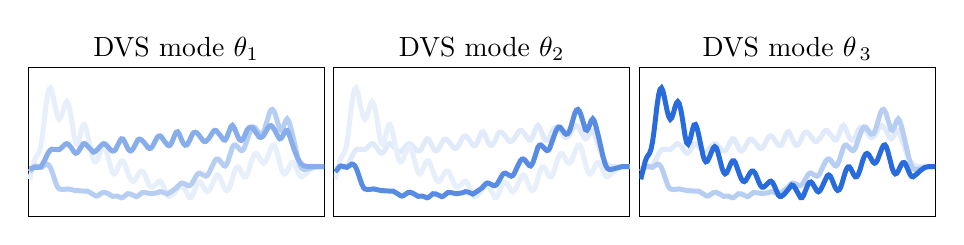
\begin{tikzpicture}

\begin{axis}[%
width=0.31\textwidth,
height=0.156\textwidth,
at={(0\textwidth,0\textwidth)},
scale only axis,
xmin=0,
xmax=200,
xtick={\empty},
ymin=-2,
ymax=4,
ytick={\empty},
axis background/.style={fill=white},
title style={yshift=-7pt},
title={DVS mode $\theta_{1}$}
]
\addplot [color=mycolor1, line width=1.8pt, forget plot]
  table[row sep=crcr]{%
1	-0.512017701432285\\
4	0.207733900905367\\
5	0.362992291907204\\
7	0.543411887664234\\
8	0.708353140959787\\
9	1.007990172039\\
10	1.4338510137197\\
12	2.45299602933548\\
13	2.8642768277434\\
14	3.1082416418551\\
15	3.1663855215526\\
16	3.04518044092282\\
17	2.79024605369548\\
18	2.48041307802799\\
19	2.20200400584608\\
20	1.99537147150252\\
21	1.90348873207662\\
22	1.96502311981934\\
23	2.14331944002069\\
24	2.36400967463479\\
25	2.54588903957668\\
26	2.61433997208346\\
27	2.53828409968483\\
28	2.32058454634904\\
29	1.98807249978606\\
31	1.21833679696618\\
32	0.960791700914911\\
33	0.902464575188645\\
34	1.01418671326752\\
35	1.23351585397376\\
36	1.49848517368608\\
37	1.67633209672843\\
38	1.69484551518406\\
39	1.56157998100031\\
40	1.32242204769781\\
43	0.46534477212731\\
44	0.278015077465511\\
45	0.191723328834854\\
46	0.214706263557304\\
47	0.32383409317336\\
50	0.754829568870463\\
51	0.803598758061241\\
52	0.757154402054738\\
53	0.607312249380186\\
56	-0.0793237049772415\\
57	-0.233413354146677\\
58	-0.292833862545052\\
59	-0.256243540023405\\
60	-0.140370287071249\\
62	0.14495833365396\\
63	0.229181594183615\\
64	0.230817937333654\\
65	0.14615504429554\\
67	-0.190043384107071\\
68	-0.361960994611934\\
69	-0.500108013740544\\
70	-0.584516929967606\\
71	-0.604986635174555\\
72	-0.562192837103225\\
74	-0.349365143297973\\
75	-0.243521730503232\\
76	-0.181889507880697\\
77	-0.179456935595454\\
78	-0.239238883002884\\
79	-0.355871533073156\\
81	-0.652706272089915\\
82	-0.768470183470953\\
83	-0.829182732046149\\
84	-0.83158589785225\\
86	-0.72986536929767\\
88	-0.605110662374386\\
89	-0.58847568847807\\
90	-0.637298968918088\\
91	-0.743046701664753\\
94	-1.15114682551601\\
95	-1.20329028102176\\
96	-1.20218334112022\\
98	-1.11481753885025\\
103	-0.745172795081771\\
104	-0.76316537027634\\
105	-0.833972099510333\\
109	-1.25075845746633\\
110	-1.25034270735875\\
111	-1.16815555725972\\
114	-0.720065725541673\\
115	-0.637604232528247\\
116	-0.62017670297891\\
117	-0.671666317857188\\
120	-0.979089330123401\\
121	-1.01632454362931\\
122	-0.977866041751213\\
123	-0.880638304934507\\
127	-0.373007593411842\\
128	-0.336911768609298\\
129	-0.374474826305999\\
130	-0.488826951342276\\
132	-0.790449115741353\\
133	-0.906409723410206\\
134	-0.961221859096185\\
135	-0.940567778226352\\
136	-0.841757860042662\\
137	-0.671236593456456\\
139	-0.262625958493544\\
140	-0.102910929498705\\
141	-0.0160324208030431\\
142	-0.0143065274480136\\
143	-0.0911279032081325\\
145	-0.338459646794377\\
146	-0.413271341129132\\
147	-0.408613677304999\\
148	-0.317648823848543\\
149	-0.157699967642429\\
151	0.241818702960131\\
152	0.402550593409359\\
153	0.503030942412295\\
154	0.528949353520659\\
155	0.485037640922116\\
158	0.177086429492817\\
159	0.134707844085312\\
160	0.167083575267242\\
161	0.266082978193026\\
163	0.584837064180135\\
164	0.743956342123283\\
165	0.850836516125838\\
166	0.872182807410212\\
167	0.788512377529543\\
168	0.608656922870409\\
171	-0.0896991966786231\\
172	-0.233213744445578\\
173	-0.295376031100147\\
174	-0.269765927218486\\
175	-0.17727832651417\\
177	0.0735468245054847\\
178	0.153916396149867\\
179	0.162388948818005\\
180	0.0928626674094062\\
183	-0.316834300047105\\
184	-0.393723692009587\\
185	-0.412143186508672\\
187	-0.325933291628019\\
190	-0.157758949059485\\
193	-0.0349148836990878\\
196	0.00295287964007684\\
200	0.00104882340659174\\
};
\addplot [color=mycolor2, line width=1.8pt, forget plot]
  table[row sep=crcr]{%
1	-0.212109764093725\\
4	0.00631551631138905\\
5	0.024655817354585\\
9	-0.030337742533959\\
12	0.0947963725573686\\
13	0.0942571399915551\\
14	0.0487193590608399\\
15	-0.0454987871963226\\
16	-0.191429830804623\\
19	-0.718884925636075\\
20	-0.836973504211301\\
21	-0.900383140398219\\
23	-0.926187401704681\\
27	-0.90031873671029\\
32	-0.964299990920722\\
38	-0.98894366356069\\
40	-0.98860657287662\\
42	-1.04924521539979\\
45	-1.16929077378603\\
46	-1.18766303545894\\
47	-1.17400355744954\\
50	-1.05103321886844\\
52	-1.0372345771809\\
54	-1.09151019477792\\
57	-1.19852548484704\\
60	-1.18799836976581\\
63	-1.25776901478761\\
64	-1.24074633736194\\
67	-1.09470770229112\\
69	-1.10331149954391\\
73	-1.21092521438737\\
74	-1.19124056580361\\
77	-1.04899297273775\\
79	-1.0475588424504\\
83	-1.09282455278966\\
87	-1.05501512434969\\
89	-1.00723341049837\\
91	-1.03187043328691\\
94	-1.10566009942943\\
96	-1.0360787344068\\
100	-0.865646359183188\\
103	-0.679296673545025\\
104	-0.659888576789683\\
106	-0.705322167208465\\
108	-0.771163225503898\\
109	-0.767813491233255\\
110	-0.726024754654929\\
111	-0.642714266786129\\
114	-0.325549838630252\\
115	-0.273385880275526\\
116	-0.262716290824528\\
118	-0.331308692118824\\
120	-0.386835609192389\\
121	-0.357209869538679\\
122	-0.277092635690252\\
124	-0.016944567233196\\
126	0.226006687375332\\
127	0.292140376591448\\
128	0.307114429319796\\
129	0.273115309471649\\
132	0.0463917078839984\\
133	0.0231421600482236\\
134	0.0860480932754513\\
135	0.223789798778228\\
138	0.784906181048626\\
139	0.862075921583425\\
140	0.868782884197287\\
142	0.762365958070632\\
143	0.686562958968324\\
144	0.644432747460939\\
145	0.660332448860828\\
146	0.744484926724596\\
148	1.09339801800024\\
150	1.41505500233805\\
151	1.53227753555169\\
152	1.59368214158067\\
153	1.58629297834361\\
155	1.43103652839307\\
156	1.34472870103968\\
157	1.30474931629337\\
158	1.31800991799639\\
159	1.39311507566006\\
160	1.5507830797676\\
163	2.16488335131194\\
164	2.27826465045732\\
165	2.30270474877992\\
166	2.23618827579472\\
167	2.09358411571219\\
170	1.49148711701514\\
171	1.45820128701635\\
172	1.5402835100216\\
174	1.85225848843731\\
175	1.92140907298526\\
176	1.84448589250312\\
177	1.66195706541941\\
179	1.18297207554753\\
182	0.386929584519351\\
183	0.175991154915522\\
184	0.0159938696478719\\
185	-0.0773392066651013\\
186	-0.116566565871494\\
188	-0.108789696732259\\
195	0.000492663385443848\\
200	0.00135427487921902\\
};
\addplot [color=mycolor3, line width=1.8pt, forget plot]
  table[row sep=crcr]{%
1	-0.0907804510253811\\
4	-0.0386648230154094\\
8	-0.0248506634210628\\
9	0.0310900876092717\\
11	0.239455832512078\\
13	0.498929580089509\\
14	0.600036324099932\\
15	0.667753614101997\\
16	0.700888163201853\\
18	0.690610100444587\\
21	0.682940279376197\\
23	0.784777318563044\\
25	0.902667693678524\\
26	0.921935015209499\\
27	0.902741223435157\\
29	0.768471445458488\\
31	0.587768975388968\\
32	0.53662494665943\\
33	0.551032036438556\\
34	0.619616307400321\\
37	0.910511225320931\\
38	0.925376384127787\\
39	0.890587852350365\\
44	0.581207945654427\\
45	0.59125106802955\\
47	0.706121049141927\\
50	0.896929752366077\\
51	0.922712649465666\\
52	0.909421992351753\\
54	0.785836595533539\\
56	0.655680717670549\\
57	0.626649080635502\\
58	0.632285865391424\\
59	0.683391475707623\\
61	0.924143728638029\\
62	1.04096070247016\\
63	1.1186303974315\\
64	1.11105225625357\\
65	1.01775065688369\\
67	0.757671628982564\\
68	0.669145076849787\\
69	0.628991867212278\\
70	0.652282506912854\\
71	0.729514478944424\\
74	1.0687031579082\\
75	1.10712268581261\\
76	1.09877037954413\\
78	0.993655116407353\\
81	0.759412192541987\\
82	0.726092137410575\\
83	0.744603803764392\\
84	0.816617893016968\\
87	1.16323632134129\\
88	1.22468426222477\\
89	1.23477419237702\\
90	1.19770771043244\\
92	1.02813905427763\\
94	0.87451417812099\\
95	0.84177666037229\\
96	0.865307152011866\\
97	0.971032042259139\\
99	1.26695264337718\\
100	1.38235600812817\\
101	1.40134553300857\\
102	1.31414254744007\\
104	1.02866483197573\\
105	0.920451344167958\\
106	0.859122998952358\\
107	0.86572705079783\\
108	0.9350001154464\\
109	1.04927650513534\\
111	1.31479372617486\\
112	1.37281908004556\\
113	1.38373173172093\\
114	1.35815430903057\\
116	1.21965874615447\\
118	1.05241630922418\\
119	1.00860409468947\\
120	1.01557175180071\\
122	1.12668272783313\\
125	1.41454767013485\\
126	1.4584867078193\\
127	1.44923124885636\\
129	1.31172373232602\\
132	1.07680894237137\\
133	1.0671923565445\\
134	1.15292701319095\\
137	1.61323604535966\\
138	1.66114772071484\\
139	1.58763133323632\\
142	1.16008151322313\\
143	1.07243910022694\\
144	1.05435374606765\\
145	1.10498778403965\\
146	1.20913848208539\\
148	1.48534660132714\\
149	1.5561863695888\\
150	1.58563539117924\\
151	1.58075215656768\\
152	1.54002260376606\\
154	1.3598230407201\\
156	1.19220194720296\\
157	1.17242623892085\\
158	1.19305565549769\\
159	1.24608127913666\\
161	1.45833457613392\\
162	1.56574934699663\\
163	1.63562105775853\\
164	1.65100061410337\\
165	1.61224785849657\\
167	1.42556734785921\\
169	1.18781853630233\\
170	1.11772876260284\\
171	1.13968804924031\\
173	1.33989726177705\\
174	1.44216258824827\\
175	1.45586371567543\\
176	1.35638326061041\\
178	0.991059613799877\\
180	0.640027090334911\\
182	0.342478216753136\\
184	0.13583700393545\\
186	0.0364945942791621\\
189	0.00154763120755774\\
200	2.90614883908802e-05\\
};
\end{axis}

\begin{axis}[%
width=0.31\textwidth,
height=0.156\textwidth,
at={(0.32\textwidth,0\textwidth)},
scale only axis,
xmin=0,
xmax=200,
xtick={\empty},
ymin=-2,
ymax=4,
ytick={\empty},
axis background/.style={fill=white},
title style={yshift=-7pt},
title={DVS mode $\theta_{2}$}
]
\addplot [color=white!75!mycolor3, line width=1.8pt, forget plot]
  table[row sep=crcr]{%
1	-0.0907804510253811\\
4	-0.0386648230154094\\
8	-0.0248506634210628\\
9	0.0310900876092717\\
11	0.239455832512078\\
13	0.498929580089509\\
14	0.600036324099932\\
15	0.667753614101997\\
16	0.700888163201853\\
18	0.690610100444587\\
21	0.682940279376197\\
23	0.784777318563044\\
25	0.902667693678524\\
26	0.921935015209499\\
27	0.902741223435157\\
29	0.768471445458488\\
31	0.587768975388968\\
32	0.53662494665943\\
33	0.551032036438556\\
34	0.619616307400321\\
37	0.910511225320931\\
38	0.925376384127787\\
39	0.890587852350365\\
44	0.581207945654427\\
45	0.59125106802955\\
47	0.706121049141927\\
50	0.896929752366077\\
51	0.922712649465666\\
52	0.909421992351753\\
54	0.785836595533539\\
56	0.655680717670549\\
57	0.626649080635502\\
58	0.632285865391424\\
59	0.683391475707623\\
61	0.924143728638029\\
62	1.04096070247016\\
63	1.1186303974315\\
64	1.11105225625357\\
65	1.01775065688369\\
67	0.757671628982564\\
68	0.669145076849787\\
69	0.628991867212278\\
70	0.652282506912854\\
71	0.729514478944424\\
74	1.0687031579082\\
75	1.10712268581261\\
76	1.09877037954413\\
78	0.993655116407353\\
81	0.759412192541987\\
82	0.726092137410575\\
83	0.744603803764392\\
84	0.816617893016968\\
87	1.16323632134129\\
88	1.22468426222477\\
89	1.23477419237702\\
90	1.19770771043244\\
92	1.02813905427763\\
94	0.87451417812099\\
95	0.84177666037229\\
96	0.865307152011866\\
97	0.971032042259139\\
99	1.26695264337718\\
100	1.38235600812817\\
101	1.40134553300857\\
102	1.31414254744007\\
104	1.02866483197573\\
105	0.920451344167958\\
106	0.859122998952358\\
107	0.86572705079783\\
108	0.9350001154464\\
109	1.04927650513534\\
111	1.31479372617486\\
112	1.37281908004556\\
113	1.38373173172093\\
114	1.35815430903057\\
116	1.21965874615447\\
118	1.05241630922418\\
119	1.00860409468947\\
120	1.01557175180071\\
122	1.12668272783313\\
125	1.41454767013485\\
126	1.4584867078193\\
127	1.44923124885636\\
129	1.31172373232602\\
132	1.07680894237137\\
133	1.0671923565445\\
134	1.15292701319095\\
137	1.61323604535966\\
138	1.66114772071484\\
139	1.58763133323632\\
142	1.16008151322313\\
143	1.07243910022694\\
144	1.05435374606765\\
145	1.10498778403965\\
146	1.20913848208539\\
148	1.48534660132714\\
149	1.5561863695888\\
150	1.58563539117924\\
151	1.58075215656768\\
152	1.54002260376606\\
154	1.3598230407201\\
156	1.19220194720296\\
157	1.17242623892085\\
158	1.19305565549769\\
159	1.24608127913666\\
161	1.45833457613392\\
162	1.56574934699663\\
163	1.63562105775853\\
164	1.65100061410337\\
165	1.61224785849657\\
167	1.42556734785921\\
169	1.18781853630233\\
170	1.11772876260284\\
171	1.13968804924031\\
173	1.33989726177705\\
174	1.44216258824827\\
175	1.45586371567543\\
176	1.35638326061041\\
178	0.991059613799877\\
180	0.640027090334911\\
182	0.342478216753136\\
184	0.13583700393545\\
186	0.0364945942791621\\
189	0.00154763120755774\\
200	2.90614883908802e-05\\
};
\addplot [color=mycolor1, line width=1.8pt, forget plot]
  table[row sep=crcr]{%
1	-0.512017701432285\\
4	0.207733900905367\\
5	0.362992291907204\\
7	0.543411887664234\\
8	0.708353140959787\\
9	1.007990172039\\
10	1.4338510137197\\
12	2.45299602933548\\
13	2.8642768277434\\
14	3.1082416418551\\
15	3.1663855215526\\
16	3.04518044092282\\
17	2.79024605369548\\
18	2.48041307802799\\
19	2.20200400584608\\
20	1.99537147150252\\
21	1.90348873207662\\
22	1.96502311981934\\
23	2.14331944002069\\
24	2.36400967463479\\
25	2.54588903957668\\
26	2.61433997208346\\
27	2.53828409968483\\
28	2.32058454634904\\
29	1.98807249978606\\
31	1.21833679696618\\
32	0.960791700914911\\
33	0.902464575188645\\
34	1.01418671326752\\
35	1.23351585397376\\
36	1.49848517368608\\
37	1.67633209672843\\
38	1.69484551518406\\
39	1.56157998100031\\
40	1.32242204769781\\
43	0.46534477212731\\
44	0.278015077465511\\
45	0.191723328834854\\
46	0.214706263557304\\
47	0.32383409317336\\
50	0.754829568870463\\
51	0.803598758061241\\
52	0.757154402054738\\
53	0.607312249380186\\
56	-0.0793237049772415\\
57	-0.233413354146677\\
58	-0.292833862545052\\
59	-0.256243540023405\\
60	-0.140370287071249\\
62	0.14495833365396\\
63	0.229181594183615\\
64	0.230817937333654\\
65	0.14615504429554\\
67	-0.190043384107071\\
68	-0.361960994611934\\
69	-0.500108013740544\\
70	-0.584516929967606\\
71	-0.604986635174555\\
72	-0.562192837103225\\
74	-0.349365143297973\\
75	-0.243521730503232\\
76	-0.181889507880697\\
77	-0.179456935595454\\
78	-0.239238883002884\\
79	-0.355871533073156\\
81	-0.652706272089915\\
82	-0.768470183470953\\
83	-0.829182732046149\\
84	-0.83158589785225\\
86	-0.72986536929767\\
88	-0.605110662374386\\
89	-0.58847568847807\\
90	-0.637298968918088\\
91	-0.743046701664753\\
94	-1.15114682551601\\
95	-1.20329028102176\\
96	-1.20218334112022\\
98	-1.11481753885025\\
103	-0.745172795081771\\
104	-0.76316537027634\\
105	-0.833972099510333\\
109	-1.25075845746633\\
110	-1.25034270735875\\
111	-1.16815555725972\\
114	-0.720065725541673\\
115	-0.637604232528247\\
116	-0.62017670297891\\
117	-0.671666317857188\\
120	-0.979089330123401\\
121	-1.01632454362931\\
122	-0.977866041751213\\
123	-0.880638304934507\\
127	-0.373007593411842\\
128	-0.336911768609298\\
129	-0.374474826305999\\
130	-0.488826951342276\\
132	-0.790449115741353\\
133	-0.906409723410206\\
134	-0.961221859096185\\
135	-0.940567778226352\\
136	-0.841757860042662\\
137	-0.671236593456456\\
139	-0.262625958493544\\
140	-0.102910929498705\\
141	-0.0160324208030431\\
142	-0.0143065274480136\\
143	-0.0911279032081325\\
145	-0.338459646794377\\
146	-0.413271341129132\\
147	-0.408613677304999\\
148	-0.317648823848543\\
149	-0.157699967642429\\
151	0.241818702960131\\
152	0.402550593409359\\
153	0.503030942412295\\
154	0.528949353520659\\
155	0.485037640922116\\
158	0.177086429492817\\
159	0.134707844085312\\
160	0.167083575267242\\
161	0.266082978193026\\
163	0.584837064180135\\
164	0.743956342123283\\
165	0.850836516125838\\
166	0.872182807410212\\
167	0.788512377529543\\
168	0.608656922870409\\
171	-0.0896991966786231\\
172	-0.233213744445578\\
173	-0.295376031100147\\
174	-0.269765927218486\\
175	-0.17727832651417\\
177	0.0735468245054847\\
178	0.153916396149867\\
179	0.162388948818005\\
180	0.0928626674094062\\
183	-0.316834300047105\\
184	-0.393723692009587\\
185	-0.412143186508672\\
187	-0.325933291628019\\
190	-0.157758949059485\\
193	-0.0349148836990878\\
196	0.00295287964007684\\
200	0.00104882340659174\\
};
\addplot [color=mycolor4, line width=1.8pt, forget plot]
  table[row sep=crcr]{%
1	-0.212109764093725\\
4	0.00631551631138905\\
5	0.024655817354585\\
9	-0.030337742533959\\
12	0.0947963725573686\\
13	0.0942571399915551\\
14	0.0487193590608399\\
15	-0.0454987871963226\\
16	-0.191429830804623\\
19	-0.718884925636075\\
20	-0.836973504211301\\
21	-0.900383140398219\\
23	-0.926187401704681\\
27	-0.90031873671029\\
32	-0.964299990920722\\
38	-0.98894366356069\\
40	-0.98860657287662\\
42	-1.04924521539979\\
45	-1.16929077378603\\
46	-1.18766303545894\\
47	-1.17400355744954\\
50	-1.05103321886844\\
52	-1.0372345771809\\
54	-1.09151019477792\\
57	-1.19852548484704\\
60	-1.18799836976581\\
63	-1.25776901478761\\
64	-1.24074633736194\\
67	-1.09470770229112\\
69	-1.10331149954391\\
73	-1.21092521438737\\
74	-1.19124056580361\\
77	-1.04899297273775\\
79	-1.0475588424504\\
83	-1.09282455278966\\
87	-1.05501512434969\\
89	-1.00723341049837\\
91	-1.03187043328691\\
94	-1.10566009942943\\
96	-1.0360787344068\\
100	-0.865646359183188\\
103	-0.679296673545025\\
104	-0.659888576789683\\
106	-0.705322167208465\\
108	-0.771163225503898\\
109	-0.767813491233255\\
110	-0.726024754654929\\
111	-0.642714266786129\\
114	-0.325549838630252\\
115	-0.273385880275526\\
116	-0.262716290824528\\
118	-0.331308692118824\\
120	-0.386835609192389\\
121	-0.357209869538679\\
122	-0.277092635690252\\
124	-0.016944567233196\\
126	0.226006687375332\\
127	0.292140376591448\\
128	0.307114429319796\\
129	0.273115309471649\\
132	0.0463917078839984\\
133	0.0231421600482236\\
134	0.0860480932754513\\
135	0.223789798778228\\
138	0.784906181048626\\
139	0.862075921583425\\
140	0.868782884197287\\
142	0.762365958070632\\
143	0.686562958968324\\
144	0.644432747460939\\
145	0.660332448860828\\
146	0.744484926724596\\
148	1.09339801800024\\
150	1.41505500233805\\
151	1.53227753555169\\
152	1.59368214158067\\
153	1.58629297834361\\
155	1.43103652839307\\
156	1.34472870103968\\
157	1.30474931629337\\
158	1.31800991799639\\
159	1.39311507566006\\
160	1.5507830797676\\
163	2.16488335131194\\
164	2.27826465045732\\
165	2.30270474877992\\
166	2.23618827579472\\
167	2.09358411571219\\
170	1.49148711701514\\
171	1.45820128701635\\
172	1.5402835100216\\
174	1.85225848843731\\
175	1.92140907298526\\
176	1.84448589250312\\
177	1.66195706541941\\
179	1.18297207554753\\
182	0.386929584519351\\
183	0.175991154915522\\
184	0.0159938696478719\\
185	-0.0773392066651013\\
186	-0.116566565871494\\
188	-0.108789696732259\\
195	0.000492663385443848\\
200	0.00135427487921902\\
};
\end{axis}

\begin{axis}[%
width=0.31\textwidth,
height=0.156\textwidth,
at={(0.64\textwidth,0\textwidth)},
scale only axis,
xmin=0,
xmax=200,
xtick={\empty},
ymin=-2,
ymax=4,
ytick={\empty},
axis background/.style={fill=white},
title style={yshift=-7pt},
title={DVS mode $\theta_{\,3}$}
]
\addplot [color=white!75!mycolor3, line width=1.8pt, forget plot]
  table[row sep=crcr]{%
1	-0.0907804510253811\\
4	-0.0386648230154094\\
8	-0.0248506634210628\\
9	0.0310900876092717\\
11	0.239455832512078\\
13	0.498929580089509\\
14	0.600036324099932\\
15	0.667753614101997\\
16	0.700888163201853\\
18	0.690610100444587\\
21	0.682940279376197\\
23	0.784777318563044\\
25	0.902667693678524\\
26	0.921935015209499\\
27	0.902741223435157\\
29	0.768471445458488\\
31	0.587768975388968\\
32	0.53662494665943\\
33	0.551032036438556\\
34	0.619616307400321\\
37	0.910511225320931\\
38	0.925376384127787\\
39	0.890587852350365\\
44	0.581207945654427\\
45	0.59125106802955\\
47	0.706121049141927\\
50	0.896929752366077\\
51	0.922712649465666\\
52	0.909421992351753\\
54	0.785836595533539\\
56	0.655680717670549\\
57	0.626649080635502\\
58	0.632285865391424\\
59	0.683391475707623\\
61	0.924143728638029\\
62	1.04096070247016\\
63	1.1186303974315\\
64	1.11105225625357\\
65	1.01775065688369\\
67	0.757671628982564\\
68	0.669145076849787\\
69	0.628991867212278\\
70	0.652282506912854\\
71	0.729514478944424\\
74	1.0687031579082\\
75	1.10712268581261\\
76	1.09877037954413\\
78	0.993655116407353\\
81	0.759412192541987\\
82	0.726092137410575\\
83	0.744603803764392\\
84	0.816617893016968\\
87	1.16323632134129\\
88	1.22468426222477\\
89	1.23477419237702\\
90	1.19770771043244\\
92	1.02813905427763\\
94	0.87451417812099\\
95	0.84177666037229\\
96	0.865307152011866\\
97	0.971032042259139\\
99	1.26695264337718\\
100	1.38235600812817\\
101	1.40134553300857\\
102	1.31414254744007\\
104	1.02866483197573\\
105	0.920451344167958\\
106	0.859122998952358\\
107	0.86572705079783\\
108	0.9350001154464\\
109	1.04927650513534\\
111	1.31479372617486\\
112	1.37281908004556\\
113	1.38373173172093\\
114	1.35815430903057\\
116	1.21965874615447\\
118	1.05241630922418\\
119	1.00860409468947\\
120	1.01557175180071\\
122	1.12668272783313\\
125	1.41454767013485\\
126	1.4584867078193\\
127	1.44923124885636\\
129	1.31172373232602\\
132	1.07680894237137\\
133	1.0671923565445\\
134	1.15292701319095\\
137	1.61323604535966\\
138	1.66114772071484\\
139	1.58763133323632\\
142	1.16008151322313\\
143	1.07243910022694\\
144	1.05435374606765\\
145	1.10498778403965\\
146	1.20913848208539\\
148	1.48534660132714\\
149	1.5561863695888\\
150	1.58563539117924\\
151	1.58075215656768\\
152	1.54002260376606\\
154	1.3598230407201\\
156	1.19220194720296\\
157	1.17242623892085\\
158	1.19305565549769\\
159	1.24608127913666\\
161	1.45833457613392\\
162	1.56574934699663\\
163	1.63562105775853\\
164	1.65100061410337\\
165	1.61224785849657\\
167	1.42556734785921\\
169	1.18781853630233\\
170	1.11772876260284\\
171	1.13968804924031\\
173	1.33989726177705\\
174	1.44216258824827\\
175	1.45586371567543\\
176	1.35638326061041\\
178	0.991059613799877\\
180	0.640027090334911\\
182	0.342478216753136\\
184	0.13583700393545\\
186	0.0364945942791621\\
189	0.00154763120755774\\
200	2.90614883908802e-05\\
};
\addplot [color=mycolor2, line width=1.8pt, forget plot]
  table[row sep=crcr]{%
1	-0.212109764093725\\
4	0.00631551631138905\\
5	0.024655817354585\\
9	-0.030337742533959\\
12	0.0947963725573686\\
13	0.0942571399915551\\
14	0.0487193590608399\\
15	-0.0454987871963226\\
16	-0.191429830804623\\
19	-0.718884925636075\\
20	-0.836973504211301\\
21	-0.900383140398219\\
23	-0.926187401704681\\
27	-0.90031873671029\\
32	-0.964299990920722\\
38	-0.98894366356069\\
40	-0.98860657287662\\
42	-1.04924521539979\\
45	-1.16929077378603\\
46	-1.18766303545894\\
47	-1.17400355744954\\
50	-1.05103321886844\\
52	-1.0372345771809\\
54	-1.09151019477792\\
57	-1.19852548484704\\
60	-1.18799836976581\\
63	-1.25776901478761\\
64	-1.24074633736194\\
67	-1.09470770229112\\
69	-1.10331149954391\\
73	-1.21092521438737\\
74	-1.19124056580361\\
77	-1.04899297273775\\
79	-1.0475588424504\\
83	-1.09282455278966\\
87	-1.05501512434969\\
89	-1.00723341049837\\
91	-1.03187043328691\\
94	-1.10566009942943\\
96	-1.0360787344068\\
100	-0.865646359183188\\
103	-0.679296673545025\\
104	-0.659888576789683\\
106	-0.705322167208465\\
108	-0.771163225503898\\
109	-0.767813491233255\\
110	-0.726024754654929\\
111	-0.642714266786129\\
114	-0.325549838630252\\
115	-0.273385880275526\\
116	-0.262716290824528\\
118	-0.331308692118824\\
120	-0.386835609192389\\
121	-0.357209869538679\\
122	-0.277092635690252\\
124	-0.016944567233196\\
126	0.226006687375332\\
127	0.292140376591448\\
128	0.307114429319796\\
129	0.273115309471649\\
132	0.0463917078839984\\
133	0.0231421600482236\\
134	0.0860480932754513\\
135	0.223789798778228\\
138	0.784906181048626\\
139	0.862075921583425\\
140	0.868782884197287\\
142	0.762365958070632\\
143	0.686562958968324\\
144	0.644432747460939\\
145	0.660332448860828\\
146	0.744484926724596\\
148	1.09339801800024\\
150	1.41505500233805\\
151	1.53227753555169\\
152	1.59368214158067\\
153	1.58629297834361\\
155	1.43103652839307\\
156	1.34472870103968\\
157	1.30474931629337\\
158	1.31800991799639\\
159	1.39311507566006\\
160	1.5507830797676\\
163	2.16488335131194\\
164	2.27826465045732\\
165	2.30270474877992\\
166	2.23618827579472\\
167	2.09358411571219\\
170	1.49148711701514\\
171	1.45820128701635\\
172	1.5402835100216\\
174	1.85225848843731\\
175	1.92140907298526\\
176	1.84448589250312\\
177	1.66195706541941\\
179	1.18297207554753\\
182	0.386929584519351\\
183	0.175991154915522\\
184	0.0159938696478719\\
185	-0.0773392066651013\\
186	-0.116566565871494\\
188	-0.108789696732259\\
195	0.000492663385443848\\
200	0.00135427487921902\\
};
\addplot [color=mycolor5, line width=1.8pt, forget plot]
  table[row sep=crcr]{%
1	-0.512017701432285\\
4	0.207733900905367\\
5	0.362992291907204\\
7	0.543411887664234\\
8	0.708353140959787\\
9	1.007990172039\\
10	1.4338510137197\\
12	2.45299602933548\\
13	2.8642768277434\\
14	3.1082416418551\\
15	3.1663855215526\\
16	3.04518044092282\\
17	2.79024605369548\\
18	2.48041307802799\\
19	2.20200400584608\\
20	1.99537147150252\\
21	1.90348873207662\\
22	1.96502311981934\\
23	2.14331944002069\\
24	2.36400967463479\\
25	2.54588903957668\\
26	2.61433997208346\\
27	2.53828409968483\\
28	2.32058454634904\\
29	1.98807249978606\\
31	1.21833679696618\\
32	0.960791700914911\\
33	0.902464575188645\\
34	1.01418671326752\\
35	1.23351585397376\\
36	1.49848517368608\\
37	1.67633209672843\\
38	1.69484551518406\\
39	1.56157998100031\\
40	1.32242204769781\\
43	0.46534477212731\\
44	0.278015077465511\\
45	0.191723328834854\\
46	0.214706263557304\\
47	0.32383409317336\\
50	0.754829568870463\\
51	0.803598758061241\\
52	0.757154402054738\\
53	0.607312249380186\\
56	-0.0793237049772415\\
57	-0.233413354146677\\
58	-0.292833862545052\\
59	-0.256243540023405\\
60	-0.140370287071249\\
62	0.14495833365396\\
63	0.229181594183615\\
64	0.230817937333654\\
65	0.14615504429554\\
67	-0.190043384107071\\
68	-0.361960994611934\\
69	-0.500108013740544\\
70	-0.584516929967606\\
71	-0.604986635174555\\
72	-0.562192837103225\\
74	-0.349365143297973\\
75	-0.243521730503232\\
76	-0.181889507880697\\
77	-0.179456935595454\\
78	-0.239238883002884\\
79	-0.355871533073156\\
81	-0.652706272089915\\
82	-0.768470183470953\\
83	-0.829182732046149\\
84	-0.83158589785225\\
86	-0.72986536929767\\
88	-0.605110662374386\\
89	-0.58847568847807\\
90	-0.637298968918088\\
91	-0.743046701664753\\
94	-1.15114682551601\\
95	-1.20329028102176\\
96	-1.20218334112022\\
98	-1.11481753885025\\
103	-0.745172795081771\\
104	-0.76316537027634\\
105	-0.833972099510333\\
109	-1.25075845746633\\
110	-1.25034270735875\\
111	-1.16815555725972\\
114	-0.720065725541673\\
115	-0.637604232528247\\
116	-0.62017670297891\\
117	-0.671666317857188\\
120	-0.979089330123401\\
121	-1.01632454362931\\
122	-0.977866041751213\\
123	-0.880638304934507\\
127	-0.373007593411842\\
128	-0.336911768609298\\
129	-0.374474826305999\\
130	-0.488826951342276\\
132	-0.790449115741353\\
133	-0.906409723410206\\
134	-0.961221859096185\\
135	-0.940567778226352\\
136	-0.841757860042662\\
137	-0.671236593456456\\
139	-0.262625958493544\\
140	-0.102910929498705\\
141	-0.0160324208030431\\
142	-0.0143065274480136\\
143	-0.0911279032081325\\
145	-0.338459646794377\\
146	-0.413271341129132\\
147	-0.408613677304999\\
148	-0.317648823848543\\
149	-0.157699967642429\\
151	0.241818702960131\\
152	0.402550593409359\\
153	0.503030942412295\\
154	0.528949353520659\\
155	0.485037640922116\\
158	0.177086429492817\\
159	0.134707844085312\\
160	0.167083575267242\\
161	0.266082978193026\\
163	0.584837064180135\\
164	0.743956342123283\\
165	0.850836516125838\\
166	0.872182807410212\\
167	0.788512377529543\\
168	0.608656922870409\\
171	-0.0896991966786231\\
172	-0.233213744445578\\
173	-0.295376031100147\\
174	-0.269765927218486\\
175	-0.17727832651417\\
177	0.0735468245054847\\
178	0.153916396149867\\
179	0.162388948818005\\
180	0.0928626674094062\\
183	-0.316834300047105\\
184	-0.393723692009587\\
185	-0.412143186508672\\
187	-0.325933291628019\\
190	-0.157758949059485\\
193	-0.0349148836990878\\
196	0.00295287964007684\\
200	0.00104882340659174\\
};
\end{axis}
\end{tikzpicture}%
 \\[0.25em]
    %% This file was created by matlab2tikz.
%
%The latest updates can be retrieved from
%  http://www.mathworks.com/matlabcentral/fileexchange/22022-matlab2tikz-matlab2tikz
%where you can also make suggestions and rate matlab2tikz.
%
\definecolor{mycolor1}{rgb}{0.90627,0.93569,0.98471}%
\definecolor{mycolor2}{rgb}{0.71882,0.80706,0.95412}%
\definecolor{mycolor3}{rgb}{0.53137,0.67843,0.92353}%
\definecolor{mycolor4}{rgb}{0.34392,0.54980,0.89294}%
\definecolor{mycolor5}{rgb}{0.15647,0.42118,0.86235}%
\definecolor{mycolor6}{rgb}{0.06275,0.35686,0.84706}%
\definecolor{mycolor7}{rgb}{0.98667,0.92118,0.91098}%
\definecolor{mycolor8}{rgb}{0.96000,0.76353,0.73294}%
\definecolor{mycolor9}{rgb}{0.93333,0.60588,0.55490}%
\definecolor{mycolor10}{rgb}{0.90667,0.44824,0.37686}%
\definecolor{mycolor11}{rgb}{0.88000,0.29059,0.19882}%
\definecolor{mycolor12}{rgb}{0.86667,0.21176,0.10980}%
\definecolor{mycolor13}{rgb}{0.91804,0.95216,0.92510}%
\definecolor{mycolor14}{rgb}{0.75412,0.85647,0.77529}%
\definecolor{mycolor15}{rgb}{0.59020,0.76078,0.62549}%
\definecolor{mycolor16}{rgb}{0.42627,0.66510,0.47569}%
\definecolor{mycolor17}{rgb}{0.26235,0.56941,0.32588}%
\definecolor{mycolor18}{rgb}{0.18039,0.52157,0.25098}%
%
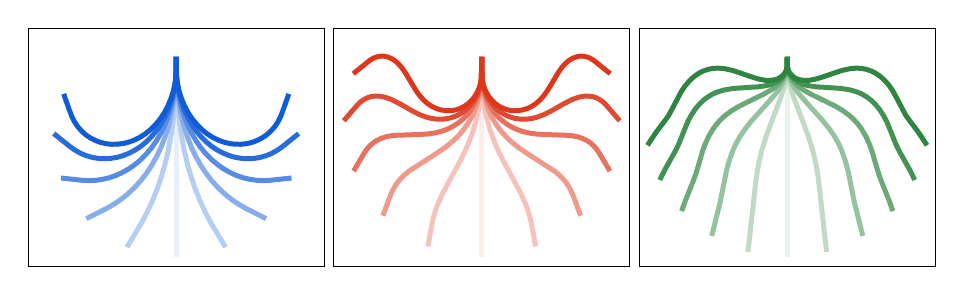
\begin{tikzpicture}

\begin{axis}[%
width=0.31\textwidth,
height=0.25\textwidth,
at={(0\textwidth,0\textwidth)},
scale only axis,
xmin=-80,
xmax=80,
xtick={\empty},
ymin=-110,
ymax=15,
ytick={\empty},
axis background/.style={fill=white},
xmajorgrids,
ymajorgrids
]
\addplot [color=mycolor1, line width=1.8pt, forget plot]
  table[row sep=crcr]{%
-0	-0\\
-3.74110697975993e-09	-105.000000000093\\
};
\addplot [color=mycolor2, line width=1.8pt, forget plot]
  table[row sep=crcr]{%
-0	-0\\
-0.161167305614711	-14.6979016016311\\
-0.724205215537552	-24.130440948486\\
-1.62484165251422	-33.0092288329655\\
-2.84391219608735	-41.3196183063557\\
-4.33983286239373	-49.050450688916\\
-6.08370480837714	-56.1898067668033\\
-8.02329978269697	-62.732687217309\\
-10.2880396765699	-69.1701626624276\\
-12.8963845981263	-75.4762175116649\\
-15.6125943796508	-81.1598503440699\\
-18.6249257861769	-86.6921487779278\\
-22.7290512138719	-93.4126180754324\\
-26.6259047319698	-99.6445592329526\\
};
\addplot [color=mycolor2, line width=1.8pt, forget plot]
  table[row sep=crcr]{%
-0	-0\\
0.16116730531246	-14.6979016016379\\
0.724205214637607	-24.130440948529\\
1.62484165100592	-33.0092288330701\\
2.84391219406344	-41.3196183065356\\
4.33983285997653	-49.0504506891717\\
6.08370480568817	-56.1898067671251\\
8.02329977979984	-62.7326872176925\\
10.2880396734375	-69.1701626628943\\
12.8963845946628	-75.4762175122693\\
15.6125943757099	-81.1598503449036\\
18.6249257815266	-86.6921487791495\\
22.729051208088	-93.4126180773471\\
26.6259047251041	-99.6445592355437\\
};
\addplot [color=mycolor3, line width=1.8pt, forget plot]
  table[row sep=crcr]{%
-0	-0\\
-0.177893259763749	-12.5966006933054\\
-0.722799877549349	-18.8723054652083\\
-1.6172652219318	-25.1077882322473\\
-2.86723713149574	-31.2817043271525\\
-4.35520972922873	-36.8608837669467\\
-6.00297555696973	-41.8447342667065\\
-8.15281158930638	-47.2032533564516\\
-10.4412041132732	-51.9271256234893\\
-13.3337988131099	-56.9240309154601\\
-16.3102592374528	-61.2475676850593\\
-19.2709663978063	-64.9286256660791\\
-22.494132356736	-68.3818183271243\\
-26.3674110900965	-71.9236914008764\\
-30.1069489334551	-74.8103679944717\\
-33.6152947038996	-77.1176148946514\\
-37.7381561765432	-79.423727386133\\
-48.1109470243421	-84.5036653552529\\
-48.5829593109394	-84.7335144535623\\
};
\addplot [color=mycolor3, line width=1.8pt, forget plot]
  table[row sep=crcr]{%
-0	-0\\
0.177893259565565	-12.5966006933118\\
0.722799877003339	-18.8723054652452\\
1.61726522096534	-25.1077882323446\\
2.8672371301023	-31.2817043273363\\
4.35520972747106	-36.8608837672274\\
6.00297555491923	-41.844734267084\\
8.15281158698366	-47.203253356938\\
10.4412041107574	-51.9271256240689\\
13.3337988104245	-56.9240309161376\\
16.3102592346297	-61.2475676858315\\
19.270966394848	-64.9286256669605\\
22.4941323536211	-68.3818183281525\\
26.3674110867562	-71.9236914021522\\
30.1069489298487	-74.8103679960935\\
33.6152947000067	-77.1176148967104\\
37.7381561722927	-79.423727388833\\
48.1109470192074	-84.5036653597581\\
48.5829593057649	-84.7335144581494\\
};
\addplot [color=mycolor4, line width=1.8pt, forget plot]
  table[row sep=crcr]{%
-0	-0\\
-0.150304668408126	-11.021676549763\\
-0.615047720310358	-15.7227967673249\\
-1.4730458810207	-20.9010846925926\\
-2.83239088840696	-26.5125449229663\\
-4.45576347512329	-31.5042921035373\\
-6.25997987798416	-35.8702342255958\\
-8.37910677923186	-40.0917972793852\\
-10.8203429289321	-44.1360000958585\\
-13.6113768299572	-47.9470892087042\\
-16.3809566877961	-51.1026808938959\\
-19.3970302670867	-54.023792212002\\
-22.6705460127614	-56.6534408652387\\
-25.7180062261556	-58.7053274633946\\
-29.3992060929905	-60.7248374310415\\
-32.7779204776504	-62.1677186337703\\
-36.2641435834314	-63.3268177998917\\
-39.8456657780698	-64.1458788202489\\
-43.484615378102	-64.6499599756908\\
-47.1557596767798	-64.7965094636445\\
-50.8260913119345	-64.6328067054671\\
-61.7921541973648	-63.4948917144393\\
-62.3142279171542	-63.4395126764606\\
};
\addplot [color=mycolor4, line width=1.8pt, forget plot]
  table[row sep=crcr]{%
-0	-0\\
0.150304668273776	-11.0216765497678\\
0.61504771995061	-15.7227967673526\\
1.4730458803411	-20.9010846926736\\
2.8323908873431	-26.5125449231404\\
4.45576347371512	-31.5042921038232\\
6.2599798762898	-35.8702342259998\\
8.37910677728618	-40.0917972799153\\
10.8203429267716	-44.136000096518\\
13.6113768276226	-47.9470892094907\\
16.3809566853418	-51.1026808947874\\
19.3970302645367	-54.0237922129921\\
22.6705460101274	-56.6534408663334\\
25.7180062234527	-58.7053274645918\\
29.3992060902059	-60.724837432388\\
32.7779204747929	-62.1677186352885\\
36.2641435804996	-63.3268178016343\\
39.8456657750681	-64.1458788222998\\
43.484615375046	-64.6499599781394\\
47.1557596737039	-64.7965094666048\\
50.8260913088855	-64.6328067090194\\
61.7921541945141	-63.4948917199021\\
62.314227914313	-63.4395126820139\\
};
\addplot [color=mycolor5, line width=1.8pt, forget plot]
  table[row sep=crcr]{%
-0	-0\\
-0.158714240849918	-10.4957380689595\\
-0.643456607656773	-14.6664630646084\\
-1.56177730776834	-19.3003428573835\\
-2.87329104506745	-23.8385656398972\\
-4.35366906790726	-27.7677103873271\\
-6.38065329246329	-32.0342062552411\\
-8.53471518723688	-35.6387537959117\\
-10.6698902899409	-38.62839593889\\
-13.3962472900377	-41.8218435722855\\
-16.042764298039	-44.3697360597515\\
-18.9045077376541	-46.6734920762282\\
-21.9894665098523	-48.6687249219677\\
-25.2474957894325	-50.3651818383069\\
-28.6707971367788	-51.6986217782939\\
-31.7009666001305	-52.5548076811513\\
-35.3228121857963	-53.1695904027016\\
-38.4656121153509	-53.3581056467778\\
-42.1351076635131	-53.1829307696389\\
-45.2430470350136	-52.6791209463755\\
-48.7813032393877	-51.6916161375571\\
-51.6953179082226	-50.4996026624502\\
-54.9151796725102	-48.7311563693139\\
-57.9207488268187	-46.6184639367124\\
-66.1937276697712	-40.1524535624561\\
};
\addplot [color=mycolor5, line width=1.8pt, forget plot]
  table[row sep=crcr]{%
-0	-0\\
0.158714240734739	-10.4957380689643\\
0.64345660735593	-14.6664630646354\\
1.56177730719449	-19.3003428574648\\
2.87329104418585	-23.8385656400675\\
4.35366906675364	-27.7677103876\\
6.38065329102	-32.0342062556515\\
8.53471518555983	-35.6387537964616\\
10.6698902880861	-38.6283959395667\\
13.3962472880089	-41.8218435731105\\
16.0427642958861	-44.3697360607052\\
18.9045077354067	-46.6734920772989\\
21.9894665075315	-48.6687249231518\\
25.2474957870576	-50.3651818395947\\
28.6707971343612	-51.6986217796914\\
31.7009665976848	-52.5548076826488\\
35.3228121833263	-53.1695904043426\\
38.4656121128726	-53.3581056485625\\
42.1351076610453	-53.182930771638\\
45.2430470325837	-52.6791209486046\\
48.7813032370528	-51.6916161401245\\
51.6953179060312	-50.4996026653665\\
54.9151796705779	-48.7311563727008\\
57.9207488252398	-46.6184639406011\\
66.193727669319	-40.1524535677865\\
};
\addplot [color=mycolor6, line width=1.8pt, forget plot]
  table[row sep=crcr]{%
-0	-0\\
-0.151941493802298	-9.97038329054241\\
-0.702860123201781	-14.1323325814535\\
-1.65361201498619	-18.2223483966822\\
-2.79949575649412	-21.7129392628167\\
-4.43546427070452	-25.5798217214961\\
-6.45250301160665	-29.2622500793775\\
-8.5118695864172	-32.3039651278895\\
-11.2089060035391	-35.5218867085713\\
-13.8628395505385	-38.0616063696407\\
-16.7486191859941	-40.3349866392992\\
-19.4230535106411	-41.9970510342485\\
-22.7232482558487	-43.6097075139492\\
-25.6998614648023	-44.637175497262\\
-28.7605771895863	-45.3760789932858\\
-31.8879766612167	-45.7407803418752\\
-35.0365074933738	-45.7763301351314\\
-38.1643228962581	-45.4187994208609\\
-41.2306386247369	-44.7036209787197\\
-43.6917729830663	-43.7939406630027\\
-46.5115024599121	-42.3926099459278\\
-48.7039018400521	-40.9512728403363\\
-51.1047024855009	-38.9141858812766\\
-53.2313868091573	-36.5935732423494\\
-55.0079531829889	-33.9943211134134\\
-56.4615464620177	-31.2018334865171\\
-57.9804093930198	-27.2867324414782\\
-60.8405264008306	-19.3885089291719\\
};
\addplot [color=mycolor6, line width=1.8pt, forget plot]
  table[row sep=crcr]{%
-0	-0\\
0.151941493705358	-9.97038329054687\\
0.702860122929252	-14.1323325814818\\
1.65361201447916	-18.2223483967652\\
2.79949575575692	-21.7129392629755\\
4.43546426970331	-25.5798217217666\\
6.45250301034821	-29.2622500797888\\
8.51186958495597	-32.3039651284381\\
11.2089060018741	-35.5218867092904\\
13.8628395487245	-38.0616063705154\\
16.7486191840595	-40.3349866403266\\
19.423053508626	-41.9970510354052\\
22.7232482537674	-43.609707515241\\
25.6998614626828	-44.6371754986642\\
28.7605771874427	-45.3760789947874\\
31.8879766590614	-45.7407803434766\\
35.0365074912174	-45.7763301368326\\
38.164322894115	-45.418799422676\\
41.2306386226231	-44.7036209806606\\
43.691772980997	-43.7939406650634\\
46.5115024579261	-42.3926099481555\\
48.7039018381705	-40.9512728427222\\
51.1047024838052	-38.9141858838808\\
53.2313868077198	-36.5935732451893\\
55.0079531819098	-33.9943211164974\\
56.4615464613765	-31.2018334898285\\
57.9804093930587	-27.2867324450532\\
60.8405264022423	-19.3885089332441\\
};
\end{axis}

\begin{axis}[%
width=0.31\textwidth,
height=0.25\textwidth,
at={(0.32\textwidth,0\textwidth)},
scale only axis,
xmin=-80,
xmax=80,
xtick={\empty},
ymin=-110,
ymax=15,
ytick={\empty},
axis background/.style={fill=white},
xmajorgrids,
ymajorgrids
]
\addplot [color=mycolor7, line width=1.8pt, forget plot]
  table[row sep=crcr]{%
-0	-0\\
-3.74110697975993e-09	-105.000000000093\\
};
\addplot [color=mycolor8, line width=1.8pt, forget plot]
  table[row sep=crcr]{%
-0	-0\\
0.179618824853662	-14.6969456963186\\
0.720365493498917	-20.9727196524908\\
1.57870665443329	-26.6825938391596\\
2.8026575190402	-32.3253293390333\\
4.40812503275563	-37.8716510558743\\
6.369975299172	-43.3022785912696\\
8.66141648607065	-48.6023022576106\\
11.7390882888001	-54.6931330108992\\
16.3809318716699	-62.9241348783482\\
21.1992500416966	-71.6570967041208\\
23.4443359293794	-76.4015782616428\\
25.1437657278726	-80.8091075743297\\
26.3086264517186	-84.8434640925158\\
27.282218742422	-89.4661633793465\\
29.0829645265034	-99.2772849867697\\
};
\addplot [color=mycolor8, line width=1.8pt, forget plot]
  table[row sep=crcr]{%
-0	-0\\
-0.179618825155856	-14.6969456963109\\
-0.72036549418263	-20.9727196524499\\
-1.57870665550803	-26.68259383906\\
-2.80265752050281	-32.3253293388497\\
-4.40812503457424	-37.8716510555879\\
-6.36997530130087	-43.3022785908713\\
-8.66141648845549	-48.6023022571019\\
-11.7390882914145	-54.6931330102748\\
-16.3809318745476	-62.9241348775753\\
-21.1992500449752	-71.6570967031279\\
-23.4443359330121	-76.4015782604835\\
-25.1437657319725	-80.8091075729912\\
-26.3086264563873	-84.8434640910138\\
-27.2822187478612	-89.4661633776828\\
-29.0829645336513	-99.2772849847924\\
};
\addplot [color=mycolor9, line width=1.8pt, forget plot]
  table[row sep=crcr]{%
-0	-0\\
0.167901752040905	-12.5965787449297\\
0.632399640443396	-16.7698232913752\\
1.43600415260799	-20.8910971685821\\
2.5994647405614	-24.9252066296352\\
4.13127803332389	-28.8345120203688\\
5.77684350528548	-32.1193204431285\\
7.99823900896773	-35.6821404564894\\
10.5507672488072	-39.0157847307572\\
13.3943406032537	-42.1049741493363\\
16.4999932019982	-44.9306402591808\\
20.2588050714796	-47.7918420292478\\
24.6534586046131	-50.6622743166056\\
39.7792729611587	-60.1193848019663\\
42.5689234468981	-62.5091408255012\\
45.0872735273563	-65.1832789379496\\
46.6388814168502	-67.299205206756\\
48.4547727224127	-70.4921647635248\\
49.8790662304233	-73.8786524672215\\
53.4213141532989	-83.2035582240078\\
};
\addplot [color=mycolor9, line width=1.8pt, forget plot]
  table[row sep=crcr]{%
-0	-0\\
-0.167901752239089	-12.596578744924\\
-0.632399640863511	-16.7698232913444\\
-1.43600415328677	-20.8910971685006\\
-2.59946474151583	-24.9252066294742\\
-4.13127803455133	-28.8345120201008\\
-5.77684350673375	-32.11932044275\\
-7.99823901064708	-35.682140455967\\
-10.5507672506841	-39.0157847300836\\
-13.3943406052961	-42.1049741485107\\
-16.4999932041742	-44.9306402582086\\
-20.2588050737667	-47.7918420281299\\
-24.6534586069951	-50.6622743153429\\
-39.779272963949	-60.1193848000625\\
-42.5689234498783	-62.509140823377\\
-45.0872735306099	-65.1832789355689\\
-46.6388814203726	-67.2992052041788\\
-48.454772726412	-70.492164760677\\
-49.8790662349971	-73.8786524641325\\
-53.4213141594969	-83.2035582203019\\
};
\addplot [color=mycolor10, line width=1.8pt, forget plot]
  table[row sep=crcr]{%
-0	-0\\
0.198689661482447	-12.06996876213\\
0.726519454106622	-15.7054775417882\\
1.63478049323484	-19.2648217660245\\
2.93086038697882	-22.7017980534257\\
4.37061053126664	-25.5021265875898\\
6.08812902575654	-28.1412965761324\\
8.08505465240323	-30.5756288266555\\
10.3452887860762	-32.7678574626365\\
12.8278403907046	-34.7045553921652\\
15.502551501093	-36.3663839130811\\
18.3315087593716	-37.749233258615\\
21.7859642235081	-38.9980603412378\\
25.3610231789425	-39.8425911994094\\
29.520812108607	-40.4134781551557\\
34.2387366011582	-40.6601041241362\\
47.8725147687173	-41.1353399535332\\
51.4904882486211	-41.7705918758114\\
53.9961557803486	-42.5490118199928\\
56.8646677729115	-43.8456507096271\\
58.6328286196918	-44.9765478438098\\
60.609754987266	-46.7011282029062\\
62.3483259386885	-48.6657379962038\\
64.0883244794099	-51.2900358882608\\
69.2555666257875	-59.8224620560758\\
};
\addplot [color=mycolor10, line width=1.8pt, forget plot]
  table[row sep=crcr]{%
-0	-0\\
-0.198689661658065	-12.0699687621237\\
-0.726519454465446	-15.7054775417549\\
-1.6347804938064	-19.2648217659367\\
-2.93086038778321	-22.70179805325\\
-4.37061053226178	-25.502126587316\\
-6.08812902693715	-28.1412965757379\\
-8.08505465374783	-30.5756288261266\\
-10.3452887875658	-32.7678574619581\\
-12.8278403923133	-34.7045553913343\\
-15.5025515027989	-36.3663839120938\\
-18.3315087611515	-37.7492332574767\\
-21.785964225349	-38.9980603399314\\
-25.3610231808182	-39.8425911979568\\
-29.5208121105036	-40.4134781535519\\
-34.2387366030626	-40.6601041223824\\
-47.8725147706442	-41.1353399512329\\
-51.4904882505892	-41.7705918732786\\
-53.9961557823815	-42.5490118172527\\
-56.8646677750749	-43.8456507065995\\
-58.6328286219909	-44.9765478405708\\
-60.6097549898066	-46.701128199391\\
-62.3483259415341	-48.6657379924191\\
-64.0883244827043	-51.2900358841789\\
-69.2555666305683	-59.8224620510936\\
};
\addplot [color=mycolor11, line width=1.8pt, forget plot]
  table[row sep=crcr]{%
-0	-0\\
0.204160151931589	-11.5445304272984\\
0.716019796924158	-14.6512352582028\\
1.59074019568521	-17.6756519074918\\
2.83444413226638	-20.5678692393208\\
4.44569861244338	-23.2720076218166\\
6.42353196590395	-25.7211717902724\\
8.31357759201906	-27.5410497200094\\
10.4145286101379	-29.1125771052781\\
12.6980226841478	-30.4048213456575\\
15.1181171028345	-31.4184279750765\\
17.6439144498901	-32.1291270128541\\
20.7562576197201	-32.60161710632\\
23.9039943141717	-32.649549649978\\
27.030675103565	-32.2839800088691\\
30.0856234872264	-31.5218150078275\\
33.5375639632223	-30.2650742455184\\
37.3180464978671	-28.4373311818088\\
44.667986316349	-24.371808647759\\
48.915640824298	-22.3080817503635\\
52.3906504313509	-21.1174530376989\\
54.9680541972697	-20.6314503475396\\
57.5901711628639	-20.5492270797656\\
59.6769157323938	-20.7736221545815\\
61.6919215858023	-21.3579272887051\\
63.5795678857968	-22.2759338815616\\
65.3284818427126	-23.4364217047074\\
67.2474896615052	-25.2245429748013\\
74.5739457639491	-33.4634382131764\\
};
\addplot [color=mycolor11, line width=1.8pt, forget plot]
  table[row sep=crcr]{%
-0	-0\\
-0.204160152085976	-11.5445304272925\\
-0.716019797224206	-14.6512352581725\\
-1.59074019615923	-17.6756519074111\\
-2.83444413292564	-20.5678692391601\\
-4.44569861328793	-23.2720076215456\\
-6.42353196691681	-25.7211717898653\\
-8.31357759315965	-27.5410497194698\\
-10.4145286113839	-29.1125771045977\\
-12.6980226854795	-30.4048213448255\\
-15.11811710423	-31.4184279740925\\
-17.6439144513278	-32.1291270117203\\
-20.7562576211846	-32.6016171050103\\
-23.9039943156388	-32.6495496485084\\
-27.0306751050153	-32.2839800072542\\
-30.0856234886468	-31.521815006092\\
-33.5375639645973	-30.2650742436581\\
-37.3180464991842	-28.4373311798288\\
-44.6679863175256	-24.3718086455245\\
-48.9156408253814	-22.3080817479356\\
-52.3906504323629	-21.1174530350615\\
-54.9680541982454	-20.6314503447073\\
-57.5901711638323	-20.5492270766901\\
-59.6769157333864	-20.7736221512832\\
-61.691921586868	-21.357927285156\\
-63.579567886993	-22.2759338777447\\
-65.3284818440872	-23.436421700622\\
-67.2474896631794	-25.2245429703948\\
-74.5739457670595	-33.4634382074927\\
};
\addplot [color=mycolor12, line width=1.8pt, forget plot]
  table[row sep=crcr]{%
-0	-0\\
0.19204617561617	-11.020191037069\\
0.631834268030758	-13.6068965503786\\
1.37927105681692	-16.1218847208177\\
2.4398788637282	-18.5215443370423\\
3.80433304756231	-20.7624292093124\\
5.46636539809623	-22.7917931363602\\
7.41174110951431	-24.5517976918284\\
9.58405058188542	-26.0222945999653\\
11.9554349123528	-27.1432697381354\\
14.4747900471449	-27.8731059338423\\
17.0748561206809	-28.2207643387791\\
19.6974273825901	-28.1680000164682\\
22.286348495042	-27.7439271757084\\
24.7895037938148	-26.958999396135\\
27.1611360580523	-25.8372300749767\\
29.3546639645105	-24.3983576448912\\
31.3432283085023	-22.6864759851999\\
33.4919335381001	-20.3847990618324\\
35.3729704314452	-17.8593597202838\\
37.893726357557	-13.8641641676335\\
41.4598957322966	-8.04604545363959\\
43.3258733244511	-5.51038587956903\\
45.4815888218366	-3.2153695586899\\
47.1078131316287	-1.88859012731494\\
48.9240107367199	-0.836971607961843\\
50.8741847520686	-0.0607405132276568\\
52.9257446323729	0.376360365797012\\
54.50002249255	0.392118098788444\\
56.5671601005495	0.0306451919429804\\
58.5456161341858	-0.668381838046557\\
60.3601182306632	-1.72263178120097\\
63.6743615863227	-4.30208626778453\\
69.4820970971107	-8.80755455786139\\
};
\addplot [color=mycolor12, line width=1.8pt, forget plot]
  table[row sep=crcr]{%
-0	-0\\
-0.192046175750463	-11.0201910370641\\
-0.631834268276478	-13.6068965503544\\
-1.37927105720026	-16.1218847207525\\
-2.4398788642544	-18.5215443369139\\
-3.80433304823686	-20.7624292090934\\
-5.46636539890983	-22.7917931360274\\
-7.41174111044835	-24.5517976913624\\
-9.58405058292301	-26.0222945993464\\
-11.9554349134662	-27.1432697373563\\
-14.4747900483068	-27.8731059328957\\
-17.0748561218652	-28.2207643376665\\
-19.6974273837713	-28.168000015199\\
-22.2863484961987	-27.7439271742895\\
-24.7895037949302	-26.9589993945838\\
-27.1611360591123	-25.8372300733084\\
-29.3546639655064	-24.3983576431249\\
-31.3432283094315	-22.686475983356\\
-33.4919335389452	-20.3847990599099\\
-35.3729704322098	-17.8593597183012\\
-37.8937263581942	-13.8641641655705\\
-41.4598957327167	-8.04604545144312\\
-43.3258733247505	-5.5103858772833\\
-45.4815888220001	-3.21536955627619\\
-47.1078131316988	-1.88859012478646\\
-48.9240107367013	-0.836971605279629\\
-50.8741847519747	-0.0607405103558278\\
-52.925744632231	0.376360368896059\\
-54.5000224924062	0.392118102087494\\
-56.5671601004572	0.0306451955353424\\
-58.5456161342011	-0.668381834150338\\
-60.3601182308539	-1.72263177700334\\
-63.6743615869656	-4.3020862630058\\
-69.4820970985361	-8.80755455207387\\
};
\end{axis}

\begin{axis}[%
width=0.31\textwidth,
height=0.25\textwidth,
at={(0.64\textwidth,0\textwidth)},
scale only axis,
xmin=-80,
xmax=80,
xtick={\empty},
ymin=-110,
ymax=15,
ytick={\empty},
axis background/.style={fill=white},
xmajorgrids,
ymajorgrids
]
\addplot [color=mycolor13, line width=1.8pt, forget plot]
  table[row sep=crcr]{%
-0	-0\\
-3.74110697975993e-09	-105.000000000093\\
};
\addplot [color=mycolor14, line width=1.8pt, forget plot]
  table[row sep=crcr]{%
-0	-0\\
-0.135147410751443	-7.34661360598231\\
-0.625512773493583	-10.9877182168633\\
-1.55242214219626	-15.0824739411295\\
-3.28952862354843	-20.5886274218602\\
-6.49484394924349	-28.9175262142738\\
-11.5917037034465	-42.1432534091495\\
-13.6721633367313	-48.6424249892323\\
-15.2084432840727	-54.7514225354963\\
-16.3748982680078	-60.9418814980342\\
-17.4287522536372	-68.7453085981102\\
-20.0081963348085	-91.6978347807509\\
-21.2841322307226	-102.119935447987\\
};
\addplot [color=mycolor14, line width=1.8pt, forget plot]
  table[row sep=crcr]{%
-0	-0\\
0.135147410725992	-7.34661360598373\\
0.625512773360214	-10.9877182168797\\
1.55242214187109	-15.08247394119\\
3.28952862288581	-20.5886274220275\\
6.49484394800551	-28.9175262146627\\
11.5917037013911	-42.1432534098542\\
13.6721633343693	-48.6424249900356\\
15.2084432814868	-54.7514225363561\\
16.3748982652253	-60.9418814989309\\
17.4287522505636	-68.7453085990459\\
20.008196329324	-91.6978347819719\\
21.2841322234222	-102.11993544943\\
};
\addplot [color=mycolor15, line width=1.8pt, forget plot]
  table[row sep=crcr]{%
-0	-0\\
-0.127341434001366	-6.29611069139661\\
-0.608754378624596	-8.87442010200422\\
-1.61994614209024	-11.8558931133011\\
-2.78122893380079	-14.2084299131829\\
-4.76224145313748	-17.3028202725877\\
-7.03484346367823	-20.1891899424672\\
-11.6130062447586	-25.2490588365077\\
-19.1376875865222	-33.3056007304772\\
-22.8168538167455	-37.7551775344313\\
-25.5344210887352	-41.6187614512388\\
-27.6259156190207	-45.2600248844999\\
-29.419224252442	-49.0563196860988\\
-31.2449776808305	-53.9771583988747\\
-32.8204270490407	-59.5323538553199\\
-34.1096349012713	-65.698720683024\\
-36.2306949529486	-75.980538712702\\
-40.8302857108623	-93.7691758828001\\
};
\addplot [color=mycolor15, line width=1.8pt, forget plot]
  table[row sep=crcr]{%
-0	-0\\
0.127341433991447	-6.29611069139735\\
0.608754378561827	-8.87442010201535\\
1.61994614192155	-11.8558931133485\\
2.78122893351879	-14.2084299132865\\
4.76224145267626	-17.3028202728062\\
7.03484346302673	-20.1891899428358\\
11.6130062437576	-25.2490588371927\\
19.1376875850005	-33.3056007316492\\
22.8168538149798	-37.7551775358054\\
25.5344210867894	-41.61876145274\\
27.6259156169349	-45.2600248860815\\
29.4192242502295	-49.0563196877406\\
31.2449776784612	-53.9771584005746\\
32.8204270464677	-59.5323538570772\\
34.1096348983902	-65.6987206848453\\
36.2306949491294	-75.9805387147206\\
40.8302857040897	-93.7691758855804\\
};
\addplot [color=mycolor16, line width=1.8pt, forget plot]
  table[row sep=crcr]{%
-0	-0\\
-0.120319502112309	-5.7708456583093\\
-0.548412697709566	-7.82460142531427\\
-1.34217916775584	-9.76746551603395\\
-2.68925350279936	-12.0178872766893\\
-4.05393706170126	-13.6122902859426\\
-6.41064885977814	-15.7007855477651\\
-8.5544118430748	-17.2133745391834\\
-12.6835447425844	-19.5093822860725\\
-16.9624750224461	-21.5120166645304\\
-25.9601047129615	-25.8136235440379\\
-30.0522747480165	-28.172960954438\\
-33.4768455970034	-30.6025218049134\\
-35.8325024286291	-32.6920008905848\\
-38.3312327427379	-35.3855539598461\\
-40.222126583339	-37.9032825339792\\
-42.4047684337579	-41.4902047698325\\
-44.2135337739883	-45.2798553444342\\
-45.7351798669961	-49.1928336965083\\
-47.8405737561464	-56.2344465666279\\
-49.5694397056843	-61.7440151591906\\
-51.0953353437054	-65.6557479884915\\
-54.904806298042	-74.8743400763716\\
-57.0944659586053	-80.7818866994531\\
};
\addplot [color=mycolor16, line width=1.8pt, forget plot]
  table[row sep=crcr]{%
-0	-0\\
0.120319502107222	-5.77084565830978\\
0.548412697673939	-7.82460142532148\\
1.3421791676641	-9.76746551606425\\
2.68925350262089	-12.0178872767718\\
4.05393706144388	-13.6122902860929\\
6.41064885940058	-15.7007855480512\\
8.55441184260151	-17.2133745396054\\
12.6835447419542	-19.5093822867765\\
16.9624750216762	-21.5120166655331\\
25.960104711916	-25.8136235456183\\
30.0522747468394	-28.1729609562471\\
33.4768455957075	-30.6025218068904\\
35.8325024272467	-32.6920008926594\\
38.331232741255	-35.385553962014\\
40.2221265817743	-37.9032825362087\\
42.4047684320785	-41.4902047721317\\
44.2135337721823	-45.2798553467936\\
45.7351798650313	-49.1928336989293\\
47.8405737537758	-56.2344465691693\\
49.5694397028051	-61.7440151618926\\
51.0953353403222	-65.6557479913912\\
54.9048062931173	-74.8743400799073\\
57.0944659526558	-80.7818867033687\\
};
\addplot [color=mycolor17, line width=1.8pt, forget plot]
  table[row sep=crcr]{%
-0	-0\\
-0.0932175019788701	-5.24673926259464\\
-0.536790539263137	-7.2960399966846\\
-1.19857104461614	-8.72455683135794\\
-2.40434474222218	-10.4421415731812\\
-3.89136008101913	-11.9219263109008\\
-5.64977977642398	-13.0665316289424\\
-8.52606409343957	-14.3468834583356\\
-11.0587837677191	-15.0285035772361\\
-15.7352651679938	-15.7002872284136\\
-19.9287895912448	-15.9259196749049\\
-29.3545175879497	-16.5651763006372\\
-34.0162943406084	-17.3246143577846\\
-37.551372594402	-18.3256039820678\\
-39.9850552581939	-19.3065432905961\\
-42.7330328901343	-20.8436685118828\\
-45.2969293383209	-22.6712995198677\\
-47.5850803352933	-24.8340120451302\\
-49.9653309142454	-27.6317611366675\\
-51.9978556733254	-30.692791064725\\
-53.7710145960405	-33.9098649605212\\
-56.0245289244812	-39.2270337856253\\
-58.825673962439	-46.0203834625668\\
-60.5046669196431	-49.2879918321205\\
-66.2666827087022	-59.2969985241939\\
-68.897131405777	-64.4387531171123\\
};
\addplot [color=mycolor17, line width=1.8pt, forget plot]
  table[row sep=crcr]{%
-0	-0\\
0.0932175019769943	-5.2467392625949\\
0.536790539238297	-7.29603999669024\\
1.19857104455652	-8.72455683137977\\
2.40434474210478	-10.4421415732437\\
3.89136008083995	-11.9219263110257\\
5.6497797761854	-13.0665316291589\\
8.52606409312625	-14.3468834587202\\
11.0587837673617	-15.0285035777852\\
15.7352651675904	-15.7002872292825\\
19.9287895908256	-15.9259196760674\\
29.3545175874898	-16.5651763024077\\
34.0162943401057	-17.3246143598195\\
37.5513725938493	-18.3256039842797\\
39.9850552575975	-19.3065432929168\\
42.7330328894781	-20.8436685143103\\
45.2969293375992	-22.6712995223873\\
47.5850803345031	-24.8340120477223\\
49.9653309133654	-27.631761139336\\
51.9978556723422	-30.6927910674618\\
53.7710145949275	-33.9098649633293\\
56.0245289230881	-39.2270337885516\\
58.825673960475	-46.0203834657309\\
60.50466691728	-49.2879918354908\\
66.2666827046843	-59.2969985285147\\
68.897131400867	-64.4387531218893\\
};
\addplot [color=mycolor18, line width=1.8pt, forget plot]
  table[row sep=crcr]{%
-0	-0\\
-0.116475123579164	-5.24490601126523\\
-0.472462056481845	-6.77792928804709\\
-1.1761081656845	-8.18559322854433\\
-2.16704006618055	-9.4091615295676\\
-3.77151589552943	-10.7604791784981\\
-5.16047113923311	-11.5011912863031\\
-7.18086417411466	-12.0665700729609\\
-9.78687841180184	-12.3716877758168\\
-11.8833117539037	-12.277973702631\\
-15.4897836876245	-11.5741975356644\\
-18.5245802182933	-10.7338703917547\\
-29.4877095394376	-7.1095200789951\\
-34.1126891138351	-6.15057511551086\\
-37.2531801074322	-5.91661636203084\\
-39.8759265855752	-5.9974086509979\\
-42.4584932919092	-6.45910130832991\\
-45.4545275624005	-7.42784139344012\\
-47.8161663452967	-8.56983158445955\\
-50.4146483719478	-10.3484581971526\\
-52.7765035665717	-12.429719380438\\
-55.1961041841115	-15.1951842039629\\
-57.0272137075763	-17.7563189722829\\
-59.3209263962525	-21.887612953906\\
-64.0863143561375	-30.6445058682447\\
-65.9670188114432	-33.1703065004312\\
-70.8158971923451	-39.3765987402663\\
-74.0876272734064	-44.1360083458769\\
-75.5495428617303	-46.3167705519935\\
};
\addplot [color=mycolor18, line width=1.8pt, forget plot]
  table[row sep=crcr]{%
-0	-0\\
0.116475123577288	-5.24490601126556\\
0.472462056465588	-6.77792928805088\\
1.17610816563914	-8.18559322856279\\
2.16704006609797	-9.40916152961624\\
3.77151589539621	-10.7604791786071\\
5.16047113906612	-11.5011912864756\\
7.18086417391717	-12.0665700732428\\
9.78687841158644	-12.371687776252\\
11.8833117536945	-12.2779737032009\\
15.4897836874634	-11.5741975364814\\
18.5245802181901	-10.7338703927807\\
29.4877095395747	-7.10952008074547\\
34.1126891140275	-6.15057511752703\\
37.2531801076365	-5.916616364207\\
39.8759265857758	-5.99740865329797\\
42.458493292091	-6.45910131073546\\
45.4545275625459	-7.42784139595851\\
47.8161663454035	-8.56983158705775\\
50.4146483719984	-10.3484581998329\\
52.7765035665556	-12.429719383194\\
55.1961041839991	-15.1951842068027\\
57.0272137073597	-17.756318975197\\
59.3209263958256	-21.8876129569365\\
64.086314354958	-30.6445058716915\\
65.9670188099264	-33.17030650413\\
70.8158971898025	-39.3765987447654\\
74.087627270035	-44.1360083509456\\
75.5495428579806	-46.3167705573158\\
};
\end{axis}
\end{tikzpicture}%

    \caption{\small (top) The first three DVS modes of the soft PneuNet actuator in vertical hanging condition, where the ordering is $\{$\ldata{Matlab1},\ldata{Matlab2},\ldata{Matlab3}$\}$. (bottom) The respective deformation for each strain mode of the PneuNet actuator. Note that these differ from the DVS basis in Section \ref{sec:C5:femPODbasis}.}
    \label{fig:C5:pneunet_modes_fem}
    \vspace{-3mm}
\end{figure}

\par To instantiate the camera class, we call \code{cam = Vision('realsense')} and establish a Secure Shell (SSH) connection with the control platform through \code{brd = Control('ip','pwd')}. Once the connection with the control platform is established, a real-time while-loop containing the necessary shape estimation algorithms to be executed. %The code for this process is provided below:

% \begin{lstlisting}[style=matlab] 
% while brd.loop(20)   % control-loop for 20 s

%     % set pressure signal
%     brd.setInput([Pressure(brd.t), 0]);
    
%     % real-time visualization
%     cam = cam.getFrame();
%     if isempty(h)
%         h = imshow(cam.lastFrame,.... 
%                    cam.WorldLimits); 
%     else
%         shp.FK(q,'Plot',true);
%         h.CData = cam.lastFrame;
%     end

%     % get color marker
%     cam = cam.getMarker(9);

%     % inverse kinematics solver
%     q = shp.IK(cam.output, q, ... 
%                'SubTask', @(s) gradPhi(s,p));               
% end
% % ------------------------------------------------
% function y = gradPhi(Shapes,p)
%   y = Shapes.Log.EL.fe + Shapes.Log.EL.fg ... 
%        - Shapes.Log.EL.G * p(1);
% end
% % ------------------------------------------------
% \end{lstlisting}

\afterpage{
\begin{figure}[!t]
    \centering
    \includegraphics*[width=0.8\textwidth]{./pdf/thesis-figure-6-34.pdf}
    %\input{./fig/fig_pneunet_estimate.tex}
    \caption{\small Real-time shape estimation using the \class{Shapes} inverse kinematics algorithm in combination with the Data-driven Variable Strain (DVS) basis. The reconstructed backbone curve is depicted in \data{magenta}. Despite the presence of substantial contact forces on the soft actuator, the shape estimation algorithm accurately reflects the behavior of the real soft robotic system. Due to the relatively small state dimension of $\dim(\q) = 3$, the algorithm achieves a bandwidth of +60 \si{\hertz}.}
    \label{fig:C5:pneunet_estimate_experiment}
    \vspace{-3mm}
\end{figure}
%
\begin{figure}[!t]
    \centering
    \includegraphics*[width=0.95\textwidth]{./pdf/thesis-figure-6-35.pdf}
    %% This file was created by matlab2tikz.
%
%The latest updates can be retrieved from
%  http://www.mathworks.com/matlabcentral/fileexchange/22022-matlab2tikz-matlab2tikz
%where you can also make suggestions and rate matlab2tikz.
%
\definecolor{mycolor1}{rgb}{0.35686,0.38039,0.41961}%
\definecolor{mycolor2}{rgb}{0.06275,0.35686,0.84706}%
\definecolor{mycolor3}{rgb}{0.86667,0.21176,0.10980}%
\definecolor{mycolor4}{rgb}{0.18039,0.52157,0.25098}%
\definecolor{mycolor5}{rgb}{1.00000,0.61569,0.11765}%
%
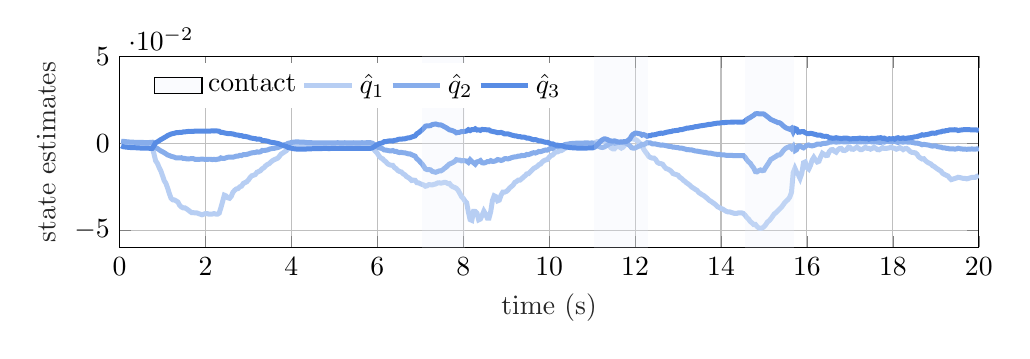
\begin{tikzpicture}

\begin{axis}[%
width=0.9\textwidth,
height=0.2\textwidth,
at={(0\textwidth,0\textwidth)},
scale only axis,
xmin=0,
xmax=20,
xlabel style={font=\color{white!15!black}},
xlabel={time (s)},
ymin=-0.06,
ymax=0.05,
ylabel style={font=\color{white!15!black}},
ylabel={state estimates},
axis background/.style={fill=white},
xmajorgrids,
ymajorgrids,
legend style={at={(0.03,0.97)}, anchor=north west, legend columns=4, legend cell align=left, align=left, draw=none}
]
\addplot[area legend, draw=none, only marks, fill=mycolor1, fill opacity=0.2, forget plot]
table[row sep=crcr] {%
x	y\\
6.82	-0.1\\
7.8	-0.1\\
7.8	0.1\\
6.82	0.1\\
}--cycle;

\addplot[area legend, draw=none, only marks, fill=mycolor5, fill opacity=0.5, forget plot]
table[row sep=crcr] {%
x	y\\
11.05	-0.1\\
12.16	-0.1\\
12.16	0.1\\
11.05	0.1\\
}--cycle;

\addplot[area legend, draw=none, only marks, fill=mycolor1, fill opacity=0.2, forget plot]
table[row sep=crcr] {%
x	y\\
14.48	-0.1\\
15.16	-0.1\\
15.16	0.1\\
14.48	0.1\\
}--cycle;

\addplot[area legend, draw=none, only marks, fill=mycolor1, fill opacity=0.2]
table[row sep=crcr] {%
x	y\\
19.36	-0.1\\
20	-0.1\\
20	0.1\\
19.36	0.1\\
}--cycle;
\addlegendentry{contact}

\addplot [color=mycolor2, line width=1.8pt]
  table[row sep=crcr]{%
0.04	-0.00103643280133061\\
0.08	-0.00081424176417978\\
0.12	-0.000734523060085178\\
0.16	-0.000752798222352151\\
0.2	-0.000770338197732011\\
0.24	-0.00078522742598501\\
0.28	-0.00086458412218092\\
0.32	-0.00078932504742905\\
0.36	-0.00080746043006687\\
0.4	-0.000816598982413327\\
0.44	-0.000889646652968652\\
0.48	-0.000881600467748443\\
0.52	-0.00088142290749971\\
0.56	-0.000883882811325817\\
0.6	-0.000886864640904118\\
0.64	-0.000889679899088399\\
0.68	-0.000892141120202294\\
0.72	-0.00113826208309237\\
0.76	-0.0025516228216988\\
0.8	-0.00588943633404928\\
0.84	-0.0100495023378977\\
0.88	-0.0114942842508347\\
0.92	-0.0138285808569815\\
0.96	-0.0158071796128859\\
1	-0.0186087546557302\\
1.04	-0.021515771934012\\
1.08	-0.0231327522660402\\
1.12	-0.0258102663513647\\
1.16	-0.0290219478968015\\
1.2	-0.0316976508744751\\
1.24	-0.0325708271162979\\
1.28	-0.0326665215679787\\
1.32	-0.0332446285645909\\
1.36	-0.0338714716007167\\
1.4	-0.0357702533114499\\
1.44	-0.03669658074501\\
1.48	-0.0371860530910634\\
1.52	-0.0371909579389351\\
1.56	-0.037779958194902\\
1.6	-0.0384805025456633\\
1.64	-0.039272991646869\\
1.68	-0.0399663689988287\\
1.72	-0.0399732816857218\\
1.76	-0.040145424523443\\
1.8	-0.0401471253579981\\
1.84	-0.0404936399549317\\
1.88	-0.0408427035588064\\
1.92	-0.0411907073831362\\
1.96	-0.0408497911129519\\
2	-0.0405009218764931\\
2.04	-0.0404974276604286\\
2.08	-0.0408429970701321\\
2.12	-0.0408464470302748\\
2.16	-0.040763013182321\\
2.2	-0.0405003757910134\\
2.24	-0.0407597404314746\\
2.28	-0.0408457154268064\\
2.32	-0.0402409767487013\\
2.36	-0.0370919824509803\\
2.4	-0.0335318095459807\\
2.44	-0.029890202014424\\
2.48	-0.0303086001149805\\
2.52	-0.0313931107278844\\
2.56	-0.0316933362613564\\
2.6	-0.0305914663663052\\
2.64	-0.0282150845131985\\
2.68	-0.0270778516943464\\
2.72	-0.0262995862904504\\
2.76	-0.026098660435443\\
2.8	-0.0251082474387974\\
2.84	-0.024680585525245\\
2.88	-0.0231692210358306\\
2.92	-0.0226662533692585\\
2.96	-0.0221956351250782\\
3	-0.0211740645244113\\
3.04	-0.019734959540904\\
3.08	-0.0187107588687751\\
3.12	-0.0184115582522419\\
3.16	-0.0180098994792376\\
3.2	-0.016710592076953\\
3.24	-0.0162676841565001\\
3.28	-0.0157644380141422\\
3.32	-0.0146805726084358\\
3.36	-0.0141077357395813\\
3.4	-0.013014884564718\\
3.44	-0.0122452095717498\\
3.48	-0.0117713947128414\\
3.52	-0.0108746051927424\\
3.56	-0.0100446164153305\\
3.6	-0.00946895557008648\\
3.64	-0.00905235671209239\\
3.68	-0.00861056950168689\\
3.72	-0.00755310664629073\\
3.76	-0.00621908327247772\\
3.8	-0.00563210904613811\\
3.84	-0.00493279418709023\\
3.88	-0.00433517006486294\\
3.92	-0.00319190958322853\\
3.96	-0.0027855361658539\\
4	-0.00226283360078229\\
4.04	-0.00201301040663637\\
4.08	-0.00178484233034612\\
4.12	-0.00142886268537042\\
4.16	-0.00118865664722164\\
4.2	-0.00107144647960287\\
4.24	-0.00107920950663255\\
4.28	-0.00108612372324225\\
4.32	-0.000917646474238803\\
4.36	-0.000806916778008004\\
4.4	-0.000872740238858923\\
4.44	-0.000910454593254878\\
4.48	-0.000931707161572209\\
4.52	-0.000860763120215568\\
4.56	-0.000796130300286942\\
4.6	-0.000911921009168224\\
4.64	-0.00100058581247214\\
4.68	-0.000987436035568176\\
4.72	-0.00080088746259409\\
4.76	-0.000821607337702085\\
4.8	-0.000928687978847063\\
4.84	-0.00101474237589183\\
4.88	-0.000998802805467266\\
4.92	-0.000896829204806583\\
4.96	-0.000805787336715808\\
5	-0.0009153492974559\\
5.04	-0.00100810742604921\\
5.08	-0.000996027982668455\\
5.12	-0.000892657940439888\\
5.16	-0.00079716155633588\\
5.2	-0.000907778256892324\\
5.24	-0.00100477047708141\\
5.28	-0.000899753199422929\\
5.32	-0.000800128872251007\\
5.36	-0.000808476072755585\\
5.4	-0.000917913519344774\\
5.44	-0.00101507283291762\\
5.48	-0.000907921463581811\\
5.52	-0.000907938555010659\\
5.56	-0.00080506954290276\\
5.6	-0.000913913409504383\\
5.64	-0.00101361188842264\\
5.68	-0.000906247360031874\\
5.72	-0.000906129486047771\\
5.76	-0.00100697981902759\\
5.8	-0.00146436057113167\\
5.84	-0.00192632056648448\\
5.88	-0.00258332944947959\\
5.92	-0.0034960173139184\\
5.96	-0.00474125297707052\\
6	-0.0057432289287665\\
6.04	-0.00729822515471524\\
6.08	-0.00840325710443711\\
6.12	-0.0088851979877553\\
6.16	-0.00991486356957607\\
6.2	-0.0106971399612174\\
6.24	-0.011798019815904\\
6.28	-0.0123718539281439\\
6.32	-0.0126432349611601\\
6.36	-0.0127186856960913\\
6.4	-0.0140499077904673\\
6.44	-0.0146580420464236\\
6.48	-0.0157365991851835\\
6.52	-0.0162482128606625\\
6.56	-0.0165513516611562\\
6.6	-0.017582454597966\\
6.64	-0.0181192943000066\\
6.68	-0.0191762608159583\\
6.72	-0.0197323641386352\\
6.76	-0.0204164526495329\\
6.8	-0.0214298461786509\\
6.84	-0.0212418851142917\\
6.88	-0.0213401704965857\\
6.92	-0.0226814057653676\\
6.96	-0.0228171063124713\\
7	-0.0232899354358515\\
7.04	-0.0237042035634871\\
7.08	-0.0240205542253887\\
7.12	-0.0247452917157538\\
7.16	-0.0244874461489468\\
7.2	-0.0238320752524805\\
7.24	-0.0239059742980851\\
7.28	-0.0239954489287557\\
7.32	-0.0236223931433356\\
7.36	-0.0234476205906231\\
7.4	-0.0228706785946847\\
7.44	-0.0227519881239502\\
7.48	-0.0229784173554057\\
7.52	-0.0227855389858697\\
7.56	-0.0224897777146501\\
7.6	-0.022631638206009\\
7.64	-0.0232086010961671\\
7.68	-0.0231674184362516\\
7.72	-0.0244415801529998\\
7.76	-0.0250969714927987\\
7.8	-0.0254232585292454\\
7.84	-0.0259791658245387\\
7.88	-0.0270324520037324\\
7.92	-0.0288283435133649\\
7.96	-0.0306835488925556\\
8	-0.0317258999514724\\
8.04	-0.0332637673410497\\
8.08	-0.034305132571764\\
8.12	-0.0396007899978177\\
8.16	-0.0439622547036696\\
8.2	-0.04439627962767\\
8.24	-0.0392476877531872\\
8.28	-0.0392910051050625\\
8.32	-0.0402674253480859\\
8.36	-0.0440978687288456\\
8.4	-0.0436305234445374\\
8.44	-0.0414571645536252\\
8.48	-0.0391015974288221\\
8.52	-0.0407890546781116\\
8.56	-0.0430972038214542\\
8.6	-0.0431199022079334\\
8.64	-0.0393171615698781\\
8.68	-0.0329447403995314\\
8.72	-0.0302639273586827\\
8.76	-0.0307523301899786\\
8.8	-0.033148997228034\\
8.84	-0.0327297576892632\\
8.88	-0.02988652432363\\
8.92	-0.0281813120354456\\
8.96	-0.0281582825754478\\
9	-0.0277851131565197\\
9.04	-0.0270066326390785\\
9.08	-0.0257806637069278\\
9.12	-0.0249507972280954\\
9.16	-0.0240709772425558\\
9.2	-0.0225776163640113\\
9.24	-0.0220082837371008\\
9.28	-0.0212486681611246\\
9.32	-0.0212409445489843\\
9.36	-0.0204613373887892\\
9.4	-0.0195180718212564\\
9.44	-0.0186961118978519\\
9.48	-0.017644179123338\\
9.52	-0.0174903395761311\\
9.56	-0.016528867966922\\
9.6	-0.0154768318467115\\
9.64	-0.0145003438696794\\
9.68	-0.0139886470402269\\
9.72	-0.013329249395455\\
9.76	-0.0123535166179151\\
9.8	-0.0119294658367839\\
9.84	-0.0107758664502927\\
9.88	-0.010011487805014\\
9.92	-0.00959476749029702\\
9.96	-0.00933121042354403\\
10	-0.00809503425373557\\
10.04	-0.00713829069285203\\
10.08	-0.00678966690679339\\
10.12	-0.00569259835383856\\
10.16	-0.00498528489988593\\
10.2	-0.00492072097943123\\
10.24	-0.00436259049305622\\
10.28	-0.0042842027174717\\
10.32	-0.00370682143696552\\
10.36	-0.0029608438706055\\
10.4	-0.00259229190498903\\
10.44	-0.00237959805799102\\
10.48	-0.00187300084863803\\
10.52	-0.00162077409682577\\
10.56	-0.00143744798571922\\
10.6	-0.00137654154179567\\
10.64	-0.00113795600719233\\
10.68	-0.00098275176371708\\
10.72	-0.000864210650195562\\
10.76	-0.000856881185092433\\
10.8	-0.000852034902252401\\
10.84	-0.00093744890951058\\
10.88	-0.000830547087257213\\
10.92	-0.000734488353785028\\
10.96	-0.000744597374956977\\
11	-0.000849529829882576\\
11.04	-0.000132652707080695\\
11.08	0.000446135632886833\\
11.12	0.000994357512732935\\
11.16	0.000912220626954346\\
11.2	0.00128246624432667\\
11.24	0.00134788294305196\\
11.28	0.00105759587208421\\
11.32	0.000599163065785264\\
11.36	-0.000404162881065013\\
11.4	-0.00128980597600534\\
11.44	-0.00262542163519088\\
11.48	-0.00320814202045427\\
11.52	-0.00318157561196136\\
11.56	-0.00198058906079325\\
11.6	-0.00176709382085166\\
11.64	-0.00218509263396361\\
11.68	-0.00280823476268483\\
11.72	-0.00226015832750655\\
11.76	-0.00108226716787422\\
11.8	0.000476874054372762\\
11.84	0.00170469790540259\\
11.88	0.00227612759793539\\
11.92	0.0026664395986747\\
11.96	0.00245077439419101\\
12	0.0022647167347039\\
12.04	0.00170029928629306\\
12.08	0.000840348470747983\\
12.12	-0.00057992330160996\\
12.16	-0.00134442428042068\\
12.2	-0.00339806201029796\\
12.24	-0.00488313118151056\\
12.28	-0.00619220248474937\\
12.32	-0.00762369403113761\\
12.36	-0.00821589290339119\\
12.4	-0.00852648780935871\\
12.44	-0.00853930311972087\\
12.48	-0.0093924217943473\\
12.52	-0.0110036516950746\\
12.56	-0.0115644273160459\\
12.6	-0.0117288180468209\\
12.64	-0.0120800254282165\\
12.68	-0.0134146924187796\\
12.72	-0.014517565557118\\
12.76	-0.0148632799182289\\
12.8	-0.0153541419218899\\
12.84	-0.016110787406102\\
12.88	-0.0173728400203863\\
12.92	-0.0177729048795208\\
12.96	-0.0180511658655473\\
13	-0.0184220165020165\\
13.04	-0.0196281179504853\\
13.08	-0.0202674293428185\\
13.12	-0.021262980171407\\
13.16	-0.0219442889697581\\
13.2	-0.0228163398783579\\
13.24	-0.0234783212867196\\
13.28	-0.0242863268562844\\
13.32	-0.025256262480764\\
13.36	-0.0258197068503223\\
13.4	-0.0265517290142288\\
13.44	-0.0270843268815921\\
13.48	-0.0282868705855018\\
13.52	-0.0289736289342022\\
13.56	-0.0296436481321181\\
13.6	-0.0301516000094606\\
13.64	-0.0309464260336277\\
13.68	-0.0317850481082145\\
13.72	-0.0327522181176539\\
13.76	-0.0333639687480751\\
13.8	-0.0340469924605356\\
13.84	-0.0347302690535281\\
13.88	-0.0355325873580903\\
13.92	-0.0365512561864087\\
13.96	-0.0370070431998405\\
14	-0.0375761594428623\\
14.04	-0.037918165133667\\
14.08	-0.0385937672282872\\
14.12	-0.0391757700862562\\
14.16	-0.0395186671442783\\
14.2	-0.0395220928225955\\
14.24	-0.0398586198902778\\
14.28	-0.0401081768565871\\
14.32	-0.0404486037548954\\
14.36	-0.0404520034500652\\
14.4	-0.0401142631271472\\
14.44	-0.0401108812833373\\
14.48	-0.0401108474644797\\
14.52	-0.0404487677621544\\
14.56	-0.0413728372350795\\
14.6	-0.0427493970027996\\
14.64	-0.0436157395569822\\
14.68	-0.0450518805524678\\
14.72	-0.0458501389289676\\
14.76	-0.0467942570219429\\
14.8	-0.0467468060268424\\
14.84	-0.0479824537717374\\
14.88	-0.0487958134858473\\
14.92	-0.0490022854966988\\
14.96	-0.048804884821437\\
15	-0.0480725091234816\\
15.04	-0.0469422235760063\\
15.08	-0.0453891589876169\\
15.12	-0.0446047760316102\\
15.16	-0.0435237738114059\\
15.2	-0.0420780165531844\\
15.24	-0.0406931144556017\\
15.28	-0.0399411090898571\\
15.32	-0.0389689564622441\\
15.36	-0.0379527229420041\\
15.4	-0.0370203216427248\\
15.44	-0.0357365676361963\\
15.48	-0.0342725352758524\\
15.52	-0.0332647958873461\\
15.56	-0.0323960212879622\\
15.6	-0.0310049023729185\\
15.64	-0.0283130758714302\\
15.68	-0.0169524673341129\\
15.72	-0.0144376852420762\\
15.76	-0.0166441079724633\\
15.8	-0.0181921370875334\\
15.84	-0.0202299625317635\\
15.88	-0.017316741813657\\
15.92	-0.0112339598200276\\
15.96	-0.0107597871488044\\
16	-0.0140776226106195\\
16.04	-0.0148887149066854\\
16.08	-0.0129067005621891\\
16.12	-0.00975644549572768\\
16.16	-0.00814182822828625\\
16.2	-0.00964188015964434\\
16.24	-0.0107714121015562\\
16.28	-0.0103587978157483\\
16.32	-0.00776961279156693\\
16.36	-0.00575707496008329\\
16.4	-0.00639195639318468\\
16.44	-0.00706096957984455\\
16.48	-0.00692982318775693\\
16.52	-0.00483670627645856\\
16.56	-0.00376348223974722\\
16.6	-0.00365286771730039\\
16.64	-0.00455949238319534\\
16.68	-0.00513338360898582\\
16.72	-0.00374646402267239\\
16.76	-0.00305288918608062\\
16.8	-0.00297719699892973\\
16.84	-0.0040545346974535\\
16.88	-0.00416337454557025\\
16.92	-0.00368841541843648\\
16.96	-0.00241221522679481\\
17	-0.00230111075992132\\
17.04	-0.00338171750821414\\
17.08	-0.0034739219470266\\
17.12	-0.00293086169642202\\
17.16	-0.00224007466653861\\
17.2	-0.00285085409298542\\
17.24	-0.00361530205032711\\
17.28	-0.00361622206496603\\
17.32	-0.00300440596679254\\
17.36	-0.00228380444190183\\
17.4	-0.00288454348574688\\
17.44	-0.00293261660181538\\
17.48	-0.00339684150448573\\
17.52	-0.00295142284261148\\
17.56	-0.00231613649069344\\
17.6	-0.00290506996947271\\
17.64	-0.00362893382369317\\
17.68	-0.00374670045355914\\
17.72	-0.00318730700837331\\
17.76	-0.00251389643633012\\
17.8	-0.00295647940102813\\
17.84	-0.00301136215211633\\
17.88	-0.00279333244696647\\
17.92	-0.00263603739685726\\
17.96	-0.00222115210863706\\
18	-0.0027840937044152\\
18.04	-0.00288825453738071\\
18.08	-0.00341409367810611\\
18.12	-0.00307370065652212\\
18.16	-0.00250911725962273\\
18.2	-0.00295466854668232\\
18.24	-0.00365163034637513\\
18.28	-0.00310970526639554\\
18.32	-0.00298007111623328\\
18.36	-0.00366066280771801\\
18.4	-0.00472864052087851\\
18.44	-0.00521119217575034\\
18.48	-0.00534403720073196\\
18.52	-0.00548903169474832\\
18.56	-0.0062535774308319\\
18.6	-0.00774332497482613\\
18.64	-0.00849153421862327\\
18.68	-0.0090543581465905\\
18.72	-0.0089198286599561\\
18.76	-0.0100497247600141\\
18.8	-0.0108382071288742\\
18.84	-0.0114123306541366\\
18.88	-0.0118442930857369\\
18.92	-0.0128332671627069\\
18.96	-0.0133354971807396\\
19	-0.014114415125969\\
19.04	-0.0148083208335903\\
19.08	-0.0154712212567796\\
19.12	-0.0160905575281527\\
19.16	-0.0173760321810221\\
19.2	-0.0178916703145913\\
19.24	-0.0184418346571784\\
19.28	-0.0188096728122462\\
19.32	-0.0199995842144708\\
19.36	-0.0209220341893638\\
19.4	-0.0206390139688507\\
19.44	-0.020263505197485\\
19.48	-0.0200144925408656\\
19.52	-0.0195898530114931\\
19.56	-0.0197598421009176\\
19.6	-0.0200094549878932\\
19.64	-0.0202571104062655\\
19.68	-0.0202595730839716\\
19.72	-0.0205021068582174\\
19.76	-0.0202620731835917\\
19.8	-0.0199382160963112\\
19.84	-0.0196847994922314\\
19.88	-0.0195990074386599\\
19.92	-0.0195981264660634\\
19.96	-0.0189921527175857\\
20	-0.0186225297706058\\
};
\addlegendentry{$\hat{q}_1$}

\addplot [color=mycolor3, line width=1.8pt]
  table[row sep=crcr]{%
0.04	0.00116446012345657\\
0.08	0.00115218997878773\\
0.12	0.00100060950830174\\
0.16	0.000884468361635358\\
0.2	0.000790493617408985\\
0.24	0.000714738841224285\\
0.28	0.000699239426404274\\
0.32	0.000613431741863724\\
0.36	0.000562919077915947\\
0.4	0.000504605891265227\\
0.44	0.000516099645211341\\
0.48	0.000494972527148432\\
0.52	0.00047102090048919\\
0.56	0.00044936215315156\\
0.6	0.000431032937461166\\
0.64	0.000415868415439587\\
0.68	0.000403400771959479\\
0.72	0.000519624532137111\\
0.76	0.000586980669633038\\
0.8	-0.000713642486005545\\
0.84	-0.00265497503795455\\
0.88	-0.00302692228127408\\
0.92	-0.00370987554382261\\
0.96	-0.00437638909334329\\
1	-0.00487423352484912\\
1.04	-0.00544376612335498\\
1.08	-0.00605260859367977\\
1.12	-0.00673651103569525\\
1.16	-0.00705611247406273\\
1.2	-0.00749702178080117\\
1.24	-0.00775336341228114\\
1.28	-0.00806456683295317\\
1.32	-0.00845237800220802\\
1.36	-0.00842435047607049\\
1.4	-0.00844027085473301\\
1.44	-0.00832228259289445\\
1.48	-0.00872963113678301\\
1.52	-0.00873367797928109\\
1.56	-0.00898588664918408\\
1.6	-0.0090592195720972\\
1.64	-0.00891195097792126\\
1.68	-0.00889112227333455\\
1.72	-0.00889068925061561\\
1.76	-0.00926250044529459\\
1.8	-0.00926622191482196\\
1.84	-0.00924112800946005\\
1.88	-0.00920419924156253\\
1.92	-0.00915525161100303\\
1.96	-0.00920353733641766\\
2	-0.00924094378090491\\
2.04	-0.00924125746598533\\
2.08	-0.00920463393789701\\
2.12	-0.00920420781100789\\
2.16	-0.00941203415776853\\
2.2	-0.00924355753171934\\
2.24	-0.00941279005112681\\
2.28	-0.00920644227506555\\
2.32	-0.00906896457865026\\
2.36	-0.00840627023102992\\
2.4	-0.00873786403078474\\
2.44	-0.00872429181601432\\
2.48	-0.00837063135123589\\
2.52	-0.00806788180297205\\
2.56	-0.00794927085811589\\
2.6	-0.0080143606118622\\
2.64	-0.00803245720778398\\
2.68	-0.00772989712699937\\
2.72	-0.00740185333743267\\
2.76	-0.00736828016686461\\
2.8	-0.00695615112780805\\
2.84	-0.00706161969766492\\
2.88	-0.00659641923918082\\
2.92	-0.00660278832956494\\
2.96	-0.00641631245684284\\
3	-0.0061512593163421\\
3.04	-0.00578187110191355\\
3.08	-0.00554739152499986\\
3.12	-0.00537532467535038\\
3.16	-0.00529600442218256\\
3.2	-0.00494629062536908\\
3.24	-0.00511230679388996\\
3.28	-0.00492077503036877\\
3.32	-0.00415468255445426\\
3.36	-0.00417030592349357\\
3.4	-0.00405266951142069\\
3.44	-0.00386937942093135\\
3.48	-0.00349497456417234\\
3.52	-0.00317102234946842\\
3.56	-0.00301525800662594\\
3.6	-0.0029253991001158\\
3.64	-0.00270280403273985\\
3.68	-0.00245263692528885\\
3.72	-0.00216918214884072\\
3.76	-0.00161980920312634\\
3.8	-0.00134192275369139\\
3.84	-0.000843772221331201\\
3.88	-0.000664430840067453\\
3.92	-1.98459419491968e-05\\
3.96	0.000122931663195266\\
4	0.00044616448062595\\
4.04	0.000656017646858242\\
4.08	0.000737315489412338\\
4.12	0.000785781745665669\\
4.16	0.000759426026854255\\
4.2	0.000705397520602139\\
4.24	0.000674047928206076\\
4.28	0.000648086659776271\\
4.32	0.00056440186669491\\
4.36	0.000416110412248826\\
4.4	0.000354119137878246\\
4.44	0.000322707916181143\\
4.48	0.000307320023032368\\
4.52	0.000264543279670708\\
4.56	0.000216452689521221\\
4.6	0.000230888873942966\\
4.64	0.000269942843957444\\
4.68	0.000286909124092888\\
4.72	0.00023476751322272\\
4.76	0.000219316501111649\\
4.8	0.000240541864638896\\
4.84	0.000280111442412887\\
4.88	0.00029796131242632\\
4.92	0.000279820016422899\\
4.96	0.000250881325891353\\
5	0.000266731433194726\\
5.04	0.000298738067131471\\
5.08	0.000311954263626695\\
5.12	0.000293924209190392\\
5.16	0.000267730686948357\\
5.2	0.000281648043380934\\
5.24	0.000309140666326449\\
5.28	0.000293366699197735\\
5.32	0.000270382558435548\\
5.36	0.000263185293255522\\
5.4	0.000278991545107243\\
5.44	0.000306200748345809\\
5.48	0.000292027405213989\\
5.52	0.000291817557333915\\
5.56	0.000272316413138626\\
5.6	0.000287143618190133\\
5.64	0.0003117955493908\\
5.68	0.00029746642971728\\
5.72	0.000297091154831499\\
5.76	0.000319396141656569\\
5.8	0.000376222320712033\\
5.84	0.000327068676508726\\
5.88	0.000105316466614016\\
5.92	-0.00046751995149055\\
5.96	-0.0013686675122871\\
6	-0.00193890078446061\\
6.04	-0.00260281985897903\\
6.08	-0.00282573238834092\\
6.12	-0.00311286969040453\\
6.16	-0.0038750437858011\\
6.2	-0.0038889878952983\\
6.24	-0.00412967402306064\\
6.28	-0.0043166403280615\\
6.32	-0.00439431006155655\\
6.36	-0.00417950661249182\\
6.4	-0.00464618164438223\\
6.44	-0.0046656942306875\\
6.48	-0.0051436938251658\\
6.52	-0.00534748593110211\\
6.56	-0.00525203270948239\\
6.6	-0.00546153532472555\\
6.64	-0.00547482984617219\\
6.68	-0.00576738288391509\\
6.72	-0.00607172508315973\\
6.76	-0.00609206122653008\\
6.8	-0.00658110904260048\\
6.84	-0.00701916954701131\\
6.88	-0.00741905577415361\\
6.92	-0.00893571660965461\\
6.96	-0.00970426490752473\\
7	-0.0107999615207831\\
7.04	-0.0118658926408573\\
7.08	-0.0132183972540799\\
7.12	-0.0147817430005709\\
7.16	-0.0151595489865863\\
7.2	-0.0151297114231012\\
7.24	-0.0153387087032595\\
7.28	-0.0162079176325777\\
7.32	-0.0164770360082437\\
7.36	-0.0166946646797931\\
7.4	-0.016330121526351\\
7.44	-0.0159373247297245\\
7.48	-0.015920109216281\\
7.52	-0.0153208785254309\\
7.56	-0.0144978382424331\\
7.6	-0.0137836561566279\\
7.64	-0.0128115086277182\\
7.68	-0.0119484695020315\\
7.72	-0.011533182478526\\
7.76	-0.0110773626894626\\
7.8	-0.0104446755651088\\
7.84	-0.00943687151891584\\
7.88	-0.00967336852530225\\
7.92	-0.00968341147909244\\
7.96	-0.0101352914923398\\
8	-0.00997041777183635\\
8.04	-0.0100852991965864\\
8.08	-0.0102593716091995\\
8.12	-0.011004269312594\\
8.16	-0.00953872919166324\\
8.2	-0.0105502930971455\\
8.24	-0.011199585001971\\
8.28	-0.0120561138932148\\
8.32	-0.0107224244406587\\
8.36	-0.0104873941727857\\
8.4	-0.00996511044165389\\
8.44	-0.0112364045118733\\
8.48	-0.0113678188689218\\
8.52	-0.011101088500428\\
8.56	-0.010584233692098\\
8.6	-0.0105760728301698\\
8.64	-0.010000894051799\\
8.68	-0.0104429013366806\\
8.72	-0.0103706396937839\\
8.76	-0.0100658447182376\\
8.8	-0.00938626650867501\\
8.84	-0.00957298394838032\\
8.88	-0.00989743605442217\\
8.92	-0.00961117922883366\\
8.96	-0.00890878244731352\\
9	-0.00887403386285891\\
9.04	-0.00900014198980126\\
9.08	-0.00874856102500952\\
9.12	-0.00831985814313311\\
9.16	-0.00803798383068712\\
9.2	-0.00783230743552163\\
9.24	-0.00775928285240045\\
9.28	-0.00739572501477353\\
9.32	-0.00739190120902539\\
9.36	-0.00699200492354975\\
9.4	-0.00713055134172335\\
9.44	-0.00696459150273599\\
9.48	-0.00645654273678098\\
9.52	-0.00651025133608717\\
9.56	-0.00616344652784596\\
9.6	-0.00571577071244969\\
9.64	-0.00542802523008466\\
9.68	-0.00560442888912061\\
9.72	-0.00523328243344721\\
9.76	-0.00472774933424781\\
9.8	-0.00478876863905501\\
9.84	-0.00449091621642274\\
9.88	-0.00410322039073621\\
9.92	-0.0038736177932081\\
9.96	-0.00390244507488681\\
10	-0.00332089510341975\\
10.04	-0.00284009137830827\\
10.08	-0.0028974804097459\\
10.12	-0.00226877316643823\\
10.16	-0.00185721831860052\\
10.2	-0.00191276396379293\\
10.24	-0.00164272097988441\\
10.28	-0.00168617581542989\\
10.32	-0.00139338476921998\\
10.36	-0.000815387364719587\\
10.4	-0.000576221633635887\\
10.44	-0.00048956075853729\\
10.48	-0.000257298345051306\\
10.52	-0.000131957295108757\\
10.56	-7.29582767736361e-05\\
10.6	-1.35549849943072e-05\\
10.64	8.85718319015185e-05\\
10.68	0.00012569214808932\\
10.72	0.000127675410217278\\
10.76	0.000140684734404443\\
10.8	0.000151724426575975\\
10.84	0.000192592840477271\\
10.88	0.00018256693807354\\
10.92	0.00016005403184491\\
10.96	0.000154341653985964\\
11	0.000176702123278302\\
11.04	-6.81069863441746e-05\\
11.08	-0.000611611588451166\\
11.12	-0.00141451636278311\\
11.16	-0.00182194946244318\\
11.2	-0.00229457620152283\\
11.24	-0.00242911646424521\\
11.28	-0.00216688577629212\\
11.32	-0.00160262563115819\\
11.36	-0.00100274495297793\\
11.4	-0.000317609254531361\\
11.44	-2.23530074679935e-05\\
11.48	0.000154988727565982\\
11.52	-2.95650869530445e-05\\
11.56	0.000212253390244454\\
11.6	0.000487979699103131\\
11.64	0.000575373002329681\\
11.68	0.000498400262615315\\
11.72	0.000417373364690804\\
11.76	0.000223542039955365\\
11.8	2.88301957393276e-05\\
11.84	-0.000637929965372069\\
11.88	-0.0014056720000763\\
11.92	-0.00256561816525906\\
11.96	-0.00281992180185707\\
12	-0.0027205849205748\\
12.04	-0.00224377722894129\\
12.08	-0.00170052196332528\\
12.12	-0.0015030849509255\\
12.16	-0.000592659713396617\\
12.2	-0.000817484630693419\\
12.24	-0.000311691437706273\\
12.28	0.000397751583323075\\
12.32	0.000166951540413692\\
12.36	0.000163484221033268\\
12.4	-0.000315432346455751\\
12.44	-0.000329383117770464\\
12.48	-0.000416892607825964\\
12.52	-0.000689741427247178\\
12.56	-0.000855303290279823\\
12.6	-0.0011043418163602\\
12.64	-0.000986566836523767\\
12.68	-0.00117287696233221\\
12.72	-0.00139263511506774\\
12.76	-0.00162219283543083\\
12.8	-0.0018110086953119\\
12.84	-0.00187251636685933\\
12.88	-0.00220104824274282\\
12.92	-0.00227792804441765\\
12.96	-0.00243601694890813\\
13	-0.00248786789571038\\
13.04	-0.00280231636085604\\
13.08	-0.00277349586826996\\
13.12	-0.00303703994449566\\
13.16	-0.00330883390677012\\
13.2	-0.00362526651004509\\
13.24	-0.00364155680636776\\
13.28	-0.00385607920819153\\
13.32	-0.00384091602085542\\
13.36	-0.00414083324780866\\
13.4	-0.00444575145639679\\
13.44	-0.00447594938469491\\
13.48	-0.00469325293707078\\
13.52	-0.00487998011868696\\
13.56	-0.00503557535087849\\
13.6	-0.00520111586785208\\
13.64	-0.00524963176948932\\
13.68	-0.0055391111576056\\
13.72	-0.00571124758251074\\
13.76	-0.00567967487371689\\
13.8	-0.00593533626025045\\
13.84	-0.00616860080976895\\
13.88	-0.0062504716208887\\
13.92	-0.00648805156019879\\
13.96	-0.00640140990085198\\
14	-0.00665301228229981\\
14.04	-0.00669207525196447\\
14.08	-0.00673777985668381\\
14.12	-0.00693610202666376\\
14.16	-0.00693047787803111\\
14.2	-0.00693036327300102\\
14.24	-0.00691165736585394\\
14.28	-0.00709275156226035\\
14.32	-0.00705886624523263\\
14.36	-0.00705846429778037\\
14.4	-0.00709450294082148\\
14.44	-0.00709480166014819\\
14.48	-0.00709480464124109\\
14.52	-0.00705910650874054\\
14.56	-0.00798141010941827\\
14.6	-0.0094921342353899\\
14.64	-0.0106824933283766\\
14.68	-0.0114766449262132\\
14.72	-0.0129868361032484\\
14.76	-0.0142255084870412\\
14.8	-0.0163383123492586\\
14.84	-0.0164651938605667\\
14.88	-0.015794398700698\\
14.92	-0.0153685296669053\\
14.96	-0.015782301190481\\
15	-0.0155695373725016\\
15.04	-0.0138705832373703\\
15.08	-0.0123855364406718\\
15.12	-0.0108981160303596\\
15.16	-0.00930388505870924\\
15.2	-0.00874863859877821\\
15.24	-0.00809855693252638\\
15.28	-0.00754290842220328\\
15.32	-0.00678752853320397\\
15.36	-0.00673119485566644\\
15.4	-0.00592551790124468\\
15.44	-0.0045398054425069\\
15.48	-0.00341745471487063\\
15.52	-0.00268087158832423\\
15.56	-0.00225668529393113\\
15.6	-0.00187376751961308\\
15.64	-0.00291869718598372\\
15.68	-0.00171359946137697\\
15.72	-0.00427007973426598\\
15.76	-0.0036666001162561\\
15.8	-0.00156560410368032\\
15.84	-0.00150378685821478\\
15.88	-0.00214343495086404\\
15.92	-0.00263226764358747\\
15.96	-0.00192173584622705\\
16	-0.00117403570837122\\
16.04	-0.000991347033039097\\
16.08	-0.00137950469628213\\
16.12	-0.00148740906682283\\
16.16	-0.00125998484106808\\
16.2	-0.000946281213443514\\
16.24	-0.000465329883917643\\
16.28	-0.000505662372186012\\
16.32	-0.000593432193443355\\
16.36	-0.000201026093158859\\
16.4	-6.09785226220033e-05\\
16.44	-3.51935259677931e-05\\
16.48	0.000190810609000914\\
16.52	0.000668732410635894\\
16.56	0.000677612361609823\\
16.6	0.00086383239586098\\
16.64	0.000883078984115849\\
16.68	0.000644006074127378\\
16.72	0.000794343411491031\\
16.76	0.000822202010053743\\
16.8	0.000979954209847757\\
16.84	0.000858114377462606\\
16.88	0.000774034035178962\\
16.92	0.000731584226932281\\
16.96	0.000809935673987429\\
17	0.00108894356079656\\
17.04	0.00106815808571522\\
17.08	0.00100115887847913\\
17.12	0.000913744771985222\\
17.16	0.000939973360340395\\
17.2	0.000764914072220699\\
17.24	0.000775124804534843\\
17.28	0.000882632323617621\\
17.32	0.000853092582190976\\
17.36	0.000904173310248355\\
17.4	0.000838110127445713\\
17.44	0.00120434940174937\\
17.48	0.000959735279888885\\
17.52	0.000792475173146982\\
17.56	0.000875490001051993\\
17.6	0.000819719313320894\\
17.64	0.000659446835690452\\
17.68	0.000564214959999764\\
17.72	0.000488993407701427\\
17.76	0.00081235499895512\\
17.8	0.000673690372742504\\
17.84	0.00113707493170656\\
17.88	0.00131565079447978\\
17.92	0.000948800481390559\\
17.96	0.00105259475625174\\
18	0.000921374876488786\\
18.04	0.0012396407501486\\
18.08	0.000743086352429932\\
18.12	0.000482590839392351\\
18.16	0.000818150980726845\\
18.2	0.000780358711122038\\
18.24	0.000640947474206136\\
18.28	0.000863250597871583\\
18.32	0.000764557165203591\\
18.36	0.000633175441336365\\
18.4	0.00062175130280599\\
18.44	0.000562675094325021\\
18.48	0.000347593988000324\\
18.52	0.000114896574793984\\
18.56	0.000150867086015736\\
18.6	-0.000146518984805964\\
18.64	-0.000394029743434929\\
18.68	-0.00084637830774752\\
18.72	-0.000619163147414927\\
18.76	-0.000794520360700647\\
18.8	-0.000909844869452499\\
18.84	-0.00109565698913242\\
18.88	-0.00142296552564776\\
18.92	-0.00164870168432786\\
18.96	-0.00148216834310862\\
19	-0.00149003822550099\\
19.04	-0.00196422469015887\\
19.08	-0.00213138905036226\\
19.12	-0.00224807042032294\\
19.16	-0.00260428416168674\\
19.2	-0.00259860060554389\\
19.24	-0.00290914833494173\\
19.28	-0.00295464193680673\\
19.32	-0.00324637427985503\\
19.36	-0.00316080638733677\\
19.4	-0.00320325940837733\\
19.44	-0.00337014721161335\\
19.48	-0.0032522475644502\\
19.52	-0.00287465544181837\\
19.56	-0.00312404226619665\\
19.6	-0.00324978542741481\\
19.64	-0.00337056487891385\\
19.68	-0.00337175349448268\\
19.72	-0.00348765013841507\\
19.76	-0.00337304016917418\\
19.8	-0.0033812307560514\\
19.84	-0.00325495366200453\\
19.88	-0.00337482426505581\\
19.92	-0.00337600117727751\\
19.96	-0.003216041080444\\
20	-0.00317210630444533\\
};
\addlegendentry{$\hat{q}_2$}

\addplot [color=mycolor4, line width=1.8pt]
  table[row sep=crcr]{%
0.04	-0.00145447361900433\\
0.08	-0.00195936431839906\\
0.12	-0.00211651479493717\\
0.16	-0.00223744351560347\\
0.2	-0.00233119069785342\\
0.24	-0.00240517743759424\\
0.28	-0.00251789680331878\\
0.32	-0.00254094098877187\\
0.36	-0.00256998360775504\\
0.4	-0.00260168387712883\\
0.44	-0.00268830083241737\\
0.48	-0.00273820016546395\\
0.52	-0.00277237817650212\\
0.56	-0.00279758310825391\\
0.6	-0.00281697984846538\\
0.64	-0.00283229362900535\\
0.68	-0.00284458696264153\\
0.72	-0.00296884923756202\\
0.76	-0.00292870130033873\\
0.8	-0.00150636330887652\\
0.84	0.000383787811878205\\
0.88	0.000765903693717286\\
0.92	0.00144915147611378\\
0.96	0.00209509744789611\\
1	0.00263763050537659\\
1.04	0.00323929832384921\\
1.08	0.0038053091275341\\
1.12	0.00447233204644595\\
1.16	0.00487509398605827\\
1.2	0.0053401820960369\\
1.24	0.00557451825316288\\
1.28	0.00580128599742358\\
1.32	0.00610901330646271\\
1.36	0.00612694169144741\\
1.4	0.00624799291953774\\
1.44	0.00622674332323801\\
1.48	0.00652511454616252\\
1.52	0.00652807437405946\\
1.56	0.00672877695630284\\
1.6	0.00682036590659464\\
1.64	0.0067799303309075\\
1.68	0.00681288344713072\\
1.72	0.00681308892921729\\
1.76	0.00705051895073897\\
1.8	0.00705288793068398\\
1.84	0.00706126216855356\\
1.88	0.0070630947898952\\
1.92	0.00705819783791784\\
1.96	0.00706285713444304\\
2	0.00706090969556564\\
2.04	0.00706085769504081\\
2.08	0.00706263778846552\\
2.12	0.0070626235854131\\
2.16	0.0071803799843243\\
2.2	0.00706146623313019\\
2.24	0.00717998413884039\\
2.28	0.00706366594456378\\
2.32	0.00693864193911187\\
2.36	0.00628011745772469\\
2.4	0.00625152611018599\\
2.44	0.00599201075223224\\
2.48	0.00575857140781441\\
2.52	0.0056005543406215\\
2.56	0.00553298313837417\\
2.6	0.00551153538210734\\
2.64	0.0053729319459409\\
2.68	0.00507982208183194\\
2.72	0.00478763143237149\\
2.76	0.00475085969567207\\
2.8	0.00437983928955791\\
2.84	0.00443653472515241\\
2.88	0.00399100303709528\\
2.92	0.00396808114925875\\
2.96	0.00379717432750611\\
3	0.00353331977763458\\
3.04	0.00316297463137223\\
3.08	0.0029219943004875\\
3.12	0.00276946587521622\\
3.16	0.00268505676883433\\
3.2	0.00233670291029614\\
3.24	0.00244586758799318\\
3.28	0.00226736719970642\\
3.32	0.00159603136022296\\
3.36	0.0015787837812434\\
3.4	0.00142795674304915\\
3.44	0.00124219618638925\\
3.48	0.000916245565825037\\
3.52	0.000608817189639684\\
3.56	0.000441332885127335\\
3.6	0.000340490169130018\\
3.64	0.000140134294237591\\
3.68	-8.47673087358856e-05\\
3.72	-0.000365577259505014\\
3.76	-0.000873797174225817\\
3.8	-0.00112960040067214\\
3.84	-0.00157862343691276\\
3.88	-0.00175975829221556\\
3.92	-0.00237412856863039\\
3.96	-0.00252612259411246\\
4	-0.00286522149598653\\
4.04	-0.00310412312392373\\
4.08	-0.00322081982528606\\
4.12	-0.00334320498559603\\
4.16	-0.00336947143876349\\
4.2	-0.00338971270252783\\
4.24	-0.00341392755817075\\
4.28	-0.00343544717359344\\
4.32	-0.00339338151304581\\
4.36	-0.00327917463286557\\
4.4	-0.00321884879541495\\
4.44	-0.00318175804919731\\
4.48	-0.00315771709251852\\
4.52	-0.00310965398409306\\
4.56	-0.00305233448102774\\
4.6	-0.00304196106128451\\
4.64	-0.00305999291565334\\
4.68	-0.00306717939252158\\
4.72	-0.00301919576693078\\
4.76	-0.00299130523147671\\
4.8	-0.00299291249456203\\
4.84	-0.00301599092988488\\
4.88	-0.0030278602235376\\
4.92	-0.00301154525515181\\
4.96	-0.00298368219180627\\
5	-0.00298514019845345\\
5.04	-0.00300458140734627\\
5.08	-0.00301461927311312\\
5.12	-0.00300093997367577\\
5.16	-0.00297858743390784\\
5.2	-0.002980671039225\\
5.24	-0.00299750722649696\\
5.28	-0.00298668200361405\\
5.32	-0.00296858402302291\\
5.36	-0.00295823294881044\\
5.4	-0.00296290375651838\\
5.44	-0.00297988441112427\\
5.48	-0.00297127502138817\\
5.52	-0.00296898588175431\\
5.56	-0.0029553739416045\\
5.6	-0.00296020402961208\\
5.64	-0.002975398445065\\
5.68	-0.00296735881499895\\
5.72	-0.0029655827493985\\
5.76	-0.00297905742894056\\
5.8	-0.00300287740295059\\
5.84	-0.00292349403097639\\
5.88	-0.00267652514907427\\
5.92	-0.00212846762932522\\
5.96	-0.00132951195714155\\
6	-0.000828599931621176\\
6.04	-0.000226903502697479\\
6.08	3.05468579755423e-06\\
6.12	0.000254386679258177\\
6.16	0.000903606733753173\\
6.2	0.000950480318542397\\
6.24	0.00119396764030833\\
6.28	0.00137015151314227\\
6.32	0.00144491547421835\\
6.36	0.00127716008627405\\
6.4	0.00171590126471375\\
6.44	0.00176127607401935\\
6.48	0.00219647552721021\\
6.52	0.00238380989743688\\
6.56	0.00232302803632331\\
6.6	0.00254112616232194\\
6.64	0.00257886365456068\\
6.68	0.0028647386555134\\
6.72	0.00313372953112089\\
6.76	0.00318468420674353\\
6.8	0.00362047837727766\\
6.84	0.00395023055263486\\
6.88	0.0042639393824819\\
6.92	0.00548773908436542\\
6.96	0.00606994607982201\\
7	0.00690425078934379\\
7.04	0.00770279022284999\\
7.08	0.00869098466786618\\
7.12	0.00983278037981672\\
7.16	0.0100854743148243\\
7.2	0.0100344925330792\\
7.24	0.0101837771052838\\
7.28	0.0107906036073108\\
7.32	0.0109595422121739\\
7.36	0.0111015015297364\\
7.4	0.0108270228569265\\
7.44	0.0105512760954775\\
7.48	0.0105487594976975\\
7.52	0.010124753818571\\
7.56	0.00953655880672226\\
7.6	0.00903763327317811\\
7.64	0.00836529584235831\\
7.68	0.00773970084236582\\
7.72	0.0074932152053163\\
7.76	0.00719080510596814\\
7.8	0.00674182936231084\\
7.84	0.00602246606990871\\
7.88	0.00625212958820686\\
7.92	0.00635073765064004\\
7.96	0.00677531732596655\\
8	0.00671583609829206\\
8.04	0.00688232940212178\\
8.08	0.00706303200871504\\
8.12	0.00782296450180853\\
8.16	0.00730311212740354\\
8.2	0.00786405750725922\\
8.24	0.00781990853612165\\
8.28	0.0083551583597008\\
8.32	0.00761406218312936\\
8.36	0.0077340563699827\\
8.4	0.00741970222975378\\
8.44	0.00798528557422892\\
8.48	0.00789028004094251\\
8.52	0.00783946879804646\\
8.56	0.00770557001253895\\
8.6	0.00770275007944608\\
8.64	0.00705235852957993\\
8.68	0.00684570374616174\\
8.72	0.00662100204035279\\
8.76	0.00643002956231781\\
8.8	0.00607688541167037\\
8.84	0.00618224218498515\\
8.88	0.00622783682153719\\
8.92	0.00591758957125019\\
8.96	0.00540017418035047\\
9	0.00535339075791008\\
9.04	0.00540219976561608\\
9.08	0.00514513922711964\\
9.12	0.00477765973336714\\
9.16	0.00451623026601951\\
9.2	0.00427683117793404\\
9.24	0.00419098889197985\\
9.28	0.00387272485083211\\
9.32	0.00386938760780296\\
9.36	0.00352062419757361\\
9.4	0.00357745573563225\\
9.44	0.0034077569397614\\
9.48	0.00296226726753048\\
9.52	0.00299632395884708\\
9.56	0.0026798438950884\\
9.6	0.00228008623647411\\
9.64	0.00200832958293563\\
9.68	0.00212043830235541\\
9.72	0.00180197741962325\\
9.76	0.00136334816663694\\
9.8	0.00139094157744552\\
9.84	0.00110931733866975\\
9.88	0.000776669385086973\\
9.92	0.00058066423955507\\
9.96	0.000591188622495846\\
10	9.29045313533896e-05\\
10.04	-0.000316414951968401\\
10.08	-0.000287527954913586\\
10.12	-0.000807720658886455\\
10.16	-0.00114948296719883\\
10.2	-0.00110995989153431\\
10.24	-0.0013355864688075\\
10.28	-0.00130614139127009\\
10.32	-0.00154527179729833\\
10.36	-0.00200629648765983\\
10.4	-0.00220241704833321\\
10.44	-0.00227660832988125\\
10.48	-0.00246661344844464\\
10.52	-0.00256726764974534\\
10.56	-0.00261511286875715\\
10.6	-0.00265947627526282\\
10.64	-0.00273234338794056\\
10.68	-0.00275145412492934\\
10.72	-0.00274072766377995\\
10.76	-0.00273565703612954\\
10.8	-0.00273061647264128\\
10.84	-0.00274996393757955\\
10.88	-0.002736098723208\\
10.92	-0.00271078086247731\\
10.96	-0.00269459718866666\\
11	-0.00269870140096639\\
11.04	-0.00247843438896691\\
11.08	-0.00185912828632936\\
11.12	-0.000774698919908063\\
11.16	0.000150477047148668\\
11.2	0.00129271434774542\\
11.24	0.00205491278007635\\
11.28	0.00250545168472579\\
11.32	0.00246220903289157\\
11.36	0.002093335685677\\
11.4	0.00154434697552558\\
11.44	0.00134938238360866\\
11.48	0.00121570987150154\\
11.52	0.00139432031515497\\
11.56	0.0010700626235024\\
11.6	0.000759956208860506\\
11.64	0.000699728347607977\\
11.68	0.000832479221441769\\
11.72	0.000874154506046389\\
11.76	0.00098585833427623\\
11.8	0.00107163351074976\\
11.84	0.0016742345387521\\
11.88	0.002553366541282\\
11.92	0.00428448341115447\\
11.96	0.0052529512063477\\
12	0.00580587570552667\\
12.04	0.00582394788121572\\
12.08	0.00553920655367965\\
12.12	0.00544688151392794\\
12.16	0.0046733105236606\\
12.2	0.00501829223762938\\
12.24	0.00463210606869467\\
12.28	0.00402240040162907\\
12.32	0.00435235886692938\\
12.36	0.00439726602689509\\
12.4	0.00487874065131467\\
12.44	0.00489284482837155\\
12.48	0.00503238362251266\\
12.52	0.00539201245633633\\
12.56	0.00558139484256605\\
12.6	0.00582001880171011\\
12.64	0.00573483106421551\\
12.68	0.00598810529606503\\
12.72	0.00625505254571733\\
12.76	0.00648181250169325\\
12.8	0.00667990415736818\\
12.84	0.00678065458669555\\
12.88	0.00714450013093944\\
12.92	0.00723584694042583\\
12.96	0.0073895415662003\\
13	0.00745693714404934\\
13.04	0.00779755914109577\\
13.08	0.00781178212590691\\
13.12	0.00809318420526137\\
13.16	0.00836073095876482\\
13.2	0.00867380734590028\\
13.24	0.0087269130279318\\
13.28	0.0089493661161573\\
13.32	0.00899489078765976\\
13.36	0.00926792263799196\\
13.4	0.00955236954725799\\
13.44	0.009608417676878\\
13.48	0.00984754647039842\\
13.52	0.0100315851514805\\
13.56	0.0101897793211815\\
13.6	0.0103446344176709\\
13.64	0.0104291981660786\\
13.68	0.0106911887732281\\
13.72	0.01087364873477\\
13.76	0.0108900767651681\\
13.8	0.0111105707156395\\
13.84	0.0113132270913846\\
13.88	0.0114192402857563\\
13.92	0.0116396057403489\\
13.96	0.0116140070370543\\
14	0.0118108447640858\\
14.04	0.0118581499261902\\
14.08	0.0119311376541559\\
14.12	0.0120895809336127\\
14.16	0.0121096994649317\\
14.2	0.0121098694117744\\
14.24	0.0121220509358266\\
14.28	0.012244322118443\\
14.32	0.0122485506037768\\
14.36	0.0122485603415188\\
14.4	0.0122453653921343\\
14.44	0.0122453012919281\\
14.48	0.0122453006477416\\
14.52	0.0122483219647611\\
14.56	0.0128238961782471\\
14.6	0.0137108675786625\\
14.64	0.0143666276653431\\
14.68	0.0148384897890809\\
14.72	0.0155490829722908\\
14.76	0.0161195999237772\\
14.8	0.0169399342912483\\
14.84	0.0171068718175867\\
14.88	0.0169841259228549\\
14.92	0.0168817610813049\\
14.96	0.016983035824192\\
15	0.0168351639453928\\
15.04	0.0160799271886967\\
15.08	0.0153000022555237\\
15.12	0.0145553294055786\\
15.16	0.0136954693445161\\
15.2	0.0132917642928797\\
15.24	0.0128249545407201\\
15.28	0.0124499638799701\\
15.32	0.0119296882783748\\
15.36	0.0118226335494499\\
15.4	0.0112461407240524\\
15.44	0.0102469061141078\\
15.48	0.00937660809591005\\
15.52	0.00878725473282951\\
15.56	0.00842101669307886\\
15.6	0.00803887209104002\\
15.64	0.00864556504405546\\
15.68	0.00650956782935781\\
15.72	0.00851571362398999\\
15.76	0.00811552187926558\\
15.8	0.00636723085621489\\
15.84	0.00643279801774782\\
15.88	0.00677506874007944\\
15.92	0.00676504620179887\\
15.96	0.00611344548666133\\
16	0.00561485323145073\\
16.04	0.00550061841666184\\
16.08	0.00571249593288217\\
16.12	0.00559698145568342\\
16.16	0.00529008486739667\\
16.2	0.00509288879489215\\
16.24	0.00471643231956104\\
16.28	0.00472626809824954\\
16.32	0.00462905431572082\\
16.36	0.00412125959360584\\
16.4	0.00402916077669366\\
16.44	0.00405026573128066\\
16.48	0.00382102460939437\\
16.52	0.00318235583125575\\
16.56	0.00308636832934796\\
16.6	0.00287698250167565\\
16.64	0.00293036030205681\\
16.68	0.00322573919138258\\
16.72	0.00295441982503739\\
16.76	0.00286429865430156\\
16.8	0.00268089365359174\\
16.84	0.00290537252533734\\
16.88	0.00300419934499574\\
16.92	0.00301047369632812\\
16.96	0.00281060589391544\\
17	0.00247404272461155\\
17.04	0.00259627540258826\\
17.08	0.00267955922945468\\
17.12	0.00272941287580003\\
17.16	0.00263360118651469\\
17.2	0.00288729730057385\\
17.24	0.00294017276342869\\
17.28	0.00282360122636416\\
17.32	0.00280287061625488\\
17.36	0.00267733530874468\\
17.4	0.00280620429140567\\
17.44	0.00239302808540323\\
17.48	0.00271423113505796\\
17.52	0.00286179029273343\\
17.56	0.00270913636261857\\
17.6	0.00282455068250436\\
17.64	0.00305857844309257\\
17.68	0.00316877750669799\\
17.72	0.00320315780552017\\
17.76	0.0027919092108757\\
17.8	0.00298387507738544\\
17.84	0.00247096665592617\\
17.88	0.00223839333040394\\
17.92	0.00266245350519546\\
17.96	0.00249923423107881\\
18	0.00270433951126656\\
18.04	0.00234674571728323\\
18.08	0.00295637132726939\\
18.12	0.00320828914875632\\
18.16	0.00279243143384355\\
18.2	0.00287358884824341\\
18.24	0.00308163506163265\\
18.28	0.00279432388888288\\
18.32	0.00289252951195997\\
18.36	0.00309011904645222\\
18.4	0.00318540316736605\\
18.44	0.0032831230569591\\
18.48	0.00351110638717367\\
18.52	0.00375319860027972\\
18.56	0.00377182886435088\\
18.6	0.0041630449021208\\
18.64	0.00444883944790562\\
18.68	0.00490813315307608\\
18.72	0.00468843516313627\\
18.76	0.00492415255512491\\
18.8	0.00508091573994457\\
18.84	0.00528759020317697\\
18.88	0.00561140003846038\\
18.92	0.00587486727908383\\
18.96	0.00575665852092438\\
19	0.00581178310942148\\
19.04	0.00627565495173192\\
19.08	0.00646294247466802\\
19.12	0.00660251861200638\\
19.16	0.00698770217965403\\
19.2	0.00701390722088647\\
19.24	0.00731274012880582\\
19.28	0.00737363294709966\\
19.32	0.00769000278885223\\
19.36	0.00767243556864781\\
19.4	0.00769017920224043\\
19.44	0.00780602407213259\\
19.48	0.00769201884581796\\
19.52	0.00734789853720717\\
19.56	0.00756879379573199\\
19.6	0.00768964541497433\\
19.64	0.00780582282429646\\
19.68	0.00780696660558903\\
19.72	0.00791838925032611\\
19.76	0.00780803930101412\\
19.8	0.00779481051164541\\
19.84	0.00767338632756847\\
19.88	0.00776869347476801\\
19.92	0.00776962680061933\\
19.96	0.00759752353758536\\
20	0.00753761361990674\\
};
\addlegendentry{$\hat{q}_3$}

\draw[draw=none, only marks, fill=mycolor1, fill opacity=0.2] (7.05,-1) rectangle ++(1,1);
\draw[draw=none, only marks, fill=mycolor1, fill opacity=0.2] (11.05,-1) rectangle ++(1.25,1);
\draw[draw=none, only marks, fill=mycolor1, fill opacity=0.2] (14.55,-1) rectangle ++(1.15,1);

\end{axis}
\end{tikzpicture}%

    %\vspace{-5mm}
    \caption{\small Evolution of the state estimations during the PneuNet experiment, where the ordering is given by $\{$\ldata{Matlab1},\ldata{Matlab2},\ldata{Matlab3}$\}$. Note that the joint variables represent the modal coefficients of the DVS basis related to curvature-bending. }
    \label{fig:C5:pneunet_estimate_experiment_state}
    %\vspace{-5mm}
\end{figure}
\clearpage
}

Figure \ref{fig:C5:pneunet_estimate_experiment} shows the experiment and overlayed on top are the real-time shape estimations from the inverse kinematics algorithm that uses a combination with the Data-driven Variable Strain (DVS) basis. Figure \ref{fig:C5:pneunet_estimate_experiment_state} shows the state trajectories and the time instance of contact. Despite the significant impact of contact forces on the soft actuator, the shape estimation algorithm qualitatively matches the deformation profile of the real soft robotic system. This is due to its relatively low state dimension of $\dim(\mathbf{q}) = 3$, enabling it to achieve a bandwidth of +60 \si{\hertz} with ease.
\vfill
